\chapter{Hidráulica Básica}

\section{Hidráulica}
\subsection{Introducción}

\begin{definition}[Hidráulica]
    Relativo a la conducción del agua, de acuerdo con su significado etimológico griego.
    La Hidráulica es la aplicación de la mecánica de fluidos en ingeniería, para diseñar 
    y construir dispositivos que funcionan con líquidos, por lo general agua o aceite.
\end{definition}

La hidráulica resuelve problemas como el flujo de fluidos por conductos y canales abiertos y el diseño de presas de embalse, bombas y turbinas. 

Se divide en \textbf{general o teórica:} 

\begin{itemize}
    \item Hidrostática
    \item Hidrodinámica
\end{itemize}

y se divide en la \textbf{Aplicada (Hidrotecnia)}: 

\begin{itemize}
    \item Hidráulica urbana: 
    \begin{itemize}
        \item Sistemas de abastecimiento de agua
        \item Sistemas de alcantarillado sanitario
        \item Sistemas de desagüe fluvial 
    \end{itemize}
    \item Hidráulica Rural o Agrícola: 
    \begin{itemize}
        \item Riego 
        \item Drenaje
    \end{itemize}
    \item Hidráulica fluvial 
    \begin{itemize}
        \item Ríos
        \item Canales
    \end{itemize}
    \item Hidráulica marítima 
    \begin{itemize}
        \item Puertos
        \item Obras marítimas en general 
    \end{itemize}
    \item Hidráulica de la industria
    \item Técnicas hidroeléctricas
\end{itemize}

No existe tal vez una rama de la ingeniería que posea una historia tan rica como la hidráulica. Precisión de disponer de agua para satisfacer necesidades básicas corporales y domésticas; utilización de vías marítimas o fluviales para el transporte y cruces de ellas; Irrigación de cultivos; defensa contra las inundaciones; aprovechamiento de la energía de corrientes; todo esto ha forzado al hombre, desde los tiempos más antiguos, a vérselas con el agua. No ha sido un trato fácil.
Actualmente, el resultado de un largo proceso de desarrollo, con repetidos intentos de explicar racionalmente lo que la naturaleza sugiere, corregidos y perfeccionados a través de observaciones y mediciones más o menos precisas. 

\subsection{Historia de la hidráulica}

Los registros más antiguos atribuyen el empleo original del riego a los egipcios a orillas del río Nilo, alrededor del año 5,000 a.C. 

En 4,000 a.C. se construye en Egipto la primera presa de la que se tiene constancia, para desviar el cauce del río Nilo y proporcionar más terreno a la ciudad de Menfis. 

En 3,750 a.C. en Babilonia se presentó la primera manifestación de alcantarillado sanitario. (Colectores de aguas negras)

En 61 a.C. se construyó el primer sistema público de abastecimiento de agua en Asiria consistente en el acueducto de Jerwan. 

Grandes acueductos fueron construidos por los Romanos en varias partes del mundo a partir de 312 a.C.

En Grecia en 250 a.c. Arquímedes enunció el principio que lleva su nombre, en su tratado sobre cuerpos flotantes, también inventó el mecanismo accionador de líquidos denominado tornillos de Arquímedes

En Grecia, en el periodo de los años 200 y 120 a.C. la bomba de pistón es una bomba reciprocante, fue entendida con el físico Ctesibius e inventada por su discípulo Hero.
%PONER IMÁGEN AQUÍ DE PEREDERENCIA

En el siglo I a.C. el arquitecto e ingeniero romano, Vitrubio inventó la rueda hidráulica horizontal, antecesor de los modernos motores hidráulicos.

En el siglo XVI, en los proyectos monumentales se encontraron varios problemas que exigieron la atención de varios filósofos, así fue como Leonardo de Vinci (1252-1519)
percibió la importancia de observaciones en ese sentido

En 1680, Johann Jordan realizó el primer diseño de una bomba centrífuga.
Luego Leonardo Eulier desarrolló la teoría y en 1818 se realizó su primera aplicación en los muelles de Boston.

%IMAGEN TUVO DE VENTURI

En el siglo XIX con el desarrollo de la producción de tubos de fierro fundido capaces de resistir presiones internas 
relativamente elevadas, con el crecimiento de las ciudades y la importancia cada vez mayor de los servicios de abastecimiento 
de agua; consecuencia del empleo de nuevas máquinas, la Hidráulica tuvo un proceso de avance rápido y acentuado. 
Las investigaciones de Osborne Reynolds, Rayleigh, 
Claude.Louis Marie Henri Navier, George Gabriel Stokes,
Adhémar Jean Claude Barré de Saint-Venant y William Froude 
constituyeron la base científica para ese progreso.

%Ecuaciones de richter
%Fokker plaint medio poroso parcialmente saturado 1957
% MKS gravitacional/ Absolutos

\subsection{Introducción a la Hidrostática}

\subsubsection{Sistema MKS absoluto}

En éste, las unidades de las magnitudes fundamentales son el metro, longitud (L), kilogramo masa ($Kg_m$)
para la masa (M) y el segundo para el tiempo (T). La unidad derivada para la fuerza ($F$) es el Newton (N) definido como la fuerza que aplicada sobre 1 $Kg_m$ le produce una aceleración de 1 $\frac{m}{s^2}$

De acuerdo con esta definición se tiene que

\begin{equation}
    1N=1Kg
\end{equation}

\subsubsection{Sistema MKS gravitacional}

Las unidades fundamentales son el metro ($m$) para la longitud (L)m el kilogramo ($Kg_f$) para la fuerza ($F$) y el segundo ($s$) para el tiempo (T).
La unidad derivada de masa ($M$ es el geokilo), el cual se define como la cantidad de masa que adquiere la aceleración gravitacional estándar $a=9.80665\frac{m}{s^2}$ cuando se le aplica una fuerza de 1 $Kg_f$ de esto se obtiene: 
\begin{equation}
    F=ma
\end{equation}

Despejando la masa y sustituyendo la aceleración de la gravedad estándar: $1Kg_m=\frac{1Kg_f}{9.80665 \frac{m}{s^2}}$ luego $1Kg_m=\frac{0.1011972kg\cdot s^2}{m}=0.101972$ geokilos o U.T.M.

Combinando las ecuaciones resultantes de los dos sistemas anteriores
\begin{align*}
    &1Kg_f=1kg_m\left(9.80665\frac{m}{s^2}\right)\\
    &1kg_f=9.80665N\\
    &1N=0.101972kg_f
\end{align*}

\begin{problem}[Una compuerta radial]
    pesa $1.78\times 10^4lb$ (S. ingles gravitacional). Obtenga su peso y masa en el sistema absoluto y en el gravitacional en el sistema MKS
\end{problem}

\textit{ Sol. }

El peso en el sistema MKS gravitacional.

Si $1lb=0.4536kg_F$ ¿Cuántos kilogramos son $1.78\times 10^4lb$?
\begin{equation*}
    1.78\times 10^4lb_f=\frac{0.4536kg_f}{1lb_f}\left(1.78\times 10^4lb_f\right)=8.074.08kg_f
\end{equation*}

La masa en el sistema gravitacional en geokilos o U.T.M. se obtiene: 
\begin{equation*}
    m=\frac{F}{g}=\frac{8.074.08kg_f}{9.81 \frac{m}{s^2}}=823.046U.T.M.
\end{equation*}

El peso en el sistema absoluto (en Newtons) se obtiene aplicando la segunda ley de Newton o directamente con el factor de conversión correspondiente. 
Si $1kg_f=9.8N$, ¿Cuántos Newtons son $8074.08kg_f$?
\begin{equation*}
    \frac{9.81N}{1kg_f}\left(8074.08kg_f\right)=79.207kN
\end{equation*}

La masa en el sistema absoluto (en $kg_m$) se obtiene también aplicando directamente el factor de conversión o usando la segunda ley de Newton.
Recordando que $1N=1kg_m\cdot \frac{m}{s^2}$. De la segunda ley de newton tenemos: 
\begin{equation*}
    \frac{F}{g}=\frac{79207kg_m\cdot \frac{m}{s^2}}{9.81\frac{m}{s^2}}=8074.08kg_m
\end{equation*}

\begin{problem}[El peso del profesor es de 83 kg]
    \begin{enumerate}
        \item Determine el peso del profesor en newtons y su masa en ambos sistemas
        \item El peso del profesor y su masa en ambos sistemas en la luna ($g_{luna}=1.62 m/s2$)
    \end{enumerate}
\end{problem}

Los $83Kg_f$ en el sistema MKS absoluto serán $83kg_f\left(9.81N(1kg_f)\right)=814.23N$.
La masa en el sistema MKS absoluto es: 
\begin{equation*}
    m=\frac{F}{g}=\frac{814.23kg_m\cdot \frac{m}{s^2}}{9.81\frac{m}{s^2}}=83Kg_m
\end{equation*}
Y en el sistema MKS gravitacional es: 
\begin{equation*}
    m=\frac{F}{g}=\frac{83kg_f}{9.81\frac{m}{s^2}}=8.46\, Geokilos
\end{equation*}

La masa es la misma que en la tierra ya que no depende de la intensidad del campo gravitacional.
El peso en el sistema MKS absoluto es: 
\begin{align*}
    &F=m\cdot a=83kg_m\left(1.62\frac{m}{s^2}\right)=135.46N\\
    &\text{Y en el sistema MKS gravitacional es: }\\
    &F=8.46Kg_fs^2/m\left(1.62\frac{m}{s^2}\right)=13.7kg_f
\end{align*}

\section{Propiedades físicas de los fluidos}

\begin{definition}[Fluido]
    Es aquel que no resiste esfuerzos tangenciales (cortantes) y se deforma tomando la forma del recipiente que lo contiene.
    Líquidos y gases. El líquido presenta una superficie libre (``horizontal'' en estado de reposo) y el gas no.
\end{definition}

La hidráulica elemental trata con los líquidos perfectos o ideales (no naturales) en los cuales se asume que se cumplen las siguientes hipótesis: 
\begin{itemize}
    \item Continuidad: Sin espacios vacíos
    \item Homogeneidad: Sin purezas
    \item Incompresibilidad: No varía su volumen ante variaciones de presión externa
    \item Isotropía: Tiene las mismas propiedades en todas direcciones
    \item Carece de forma propia y toca toda forma de recipiente que lo contiene 
    \item Antiviscosidad: No ofrece resistencia a deformarse.
\end{itemize}

En los líquidos reales, no se cumplen las hipótesis mencionadas, es decir son: Discontinuos heterogéneas, compresibles, anisótropos y viscosos.

\subsection{Peso específico }

\begin{definition}[Peso específico]
    Es el peso por unidad de volumen de una sustancia. También conocido como peso volumétrico. Sus dimensiones son ($FL^{-3}$). Varía con la temperatura
    \begin{equation}
        \omega=\frac{Peso}{Volumen}
    \end{equation}
\end{definition}

El valor estándar del peso específico del agua para diseño de obras hidráulicas son: 
\begin{align*}
    &\omega_{H2O}=1,000\frac{kg}{m^3}&& \text{Sistema gravitacional MKS a }4^{\circ}C\\
    &\omega_{H2O}=9.810\frac{N}{m^3}&& \text{Sistema absoluto MKS}\\
    &\omega_{Hg}=13.595\frac{kg}{m^3}&& \text{Sistema gravitacional MKS}\\
    &\omega_{Cu}=8.900\frac{kg}{m^3}&& \text{Sistema absoluto MKS}\\
    &\omega_{Al}=2.700\frac{kg}{m^3}&& \text{Sistema absoluto MKS}
\end{align*}

\begin{table}[h!]
    \centering\begin{tabular}{@{}ccccc@{}}
        \toprule
        \begin{tabular}[c]{@{}c@{}}Temperatura\\ $(C^{\circ})$\end{tabular} & \begin{tabular}[c]{@{}c@{}}Peso específico\\ $(\frac{kg}{m^3})$\end{tabular} & \begin{tabular}[c]{@{}c@{}}Viscosidad\\ Cinemática\\ $(10^{-6}m^2/s)$\end{tabular} & \begin{tabular}[c]{@{}c@{}}Tensión \\ superficial\\ $(10^{-3}kg/m)$\end{tabular} & \begin{tabular}[c]{@{}c@{}}Módulo de \\ Elasticidad\\ $(10^8kg/m^2)$\end{tabular} \\ \midrule
        0                                                                   & 999.9                                                                & 1.77                                                                               & 7.71                                                                             & 2.03                                                                               \\
        4                                                                   & 1,000                                                                & 1.57                                                                               & 7.66                                                                             & 2.07                                                                               \\
        10                                                                  & 999.7                                                                & 1.31                                                                               & 7.57                                                                             & 2.14                                                                               \\
        20                                                                  & 998.2                                                                & 1.01                                                                               & 7.43                                                                             & 2.23                                                                               \\
        30                                                                  & 992.7                                                                & 0.83                                                                               & 7.26                                                                             & 2.30                                                                               \\
        40                                                                  & 992.2                                                                & 0.66                                                                               & 7.10                                                                             & 2.33                                                                               \\
        50                                                                  & 988.1                                                                & 0.55                                                                               & 6.90                                                                             & 2.34                                                                               \\
        60                                                                  & 983.2                                                                & 0.46                                                                               & 6.76                                                                             & 2.32                                                                               \\
        80                                                                  & 971.8                                                                & 0.37                                                                               & 6.38                                                                             & 2.24                                                                               \\
        100                                                                 & 958.4                                                                & 0.29                                                                               & 6.00                                                                             & 2.13                                                                               \\ \bottomrule
    \end{tabular}
    \caption{Propiedades físicas del agua a presión atmosférica normal en función de la temperatura}
    \label{tabhb1}
    \end{table}

\subsection{Densidad}

La densidad es masa por unidad de volumen de una sustancia. Sus dimensiones son ($ML^{-3}$) en el sistema absoluto y ($FT^2L^{-4}$) en el sistema gravitacional: 
\begin{equation}
    \rho=\frac{masa}{volumen}
\end{equation}

Las dos propiedades anteriores se relacionan mediante la ley: $\omega=g\cdot\rho$ que resulta de aplicar la segunda ley de Newton a la unidad de volumen de fluido: 

\begin{equation}
    \frac{F}{Vol}=\frac{M\cdot a}{Vol}
\end{equation}
\begin{align*}
    &\rho_{4^{\circ}C}=\frac{1,000\frac{kg}{m^3}}{9.81kg\cdot s^2/m^2}=101.94kg\cdot s^2/m^4&&\text{Sistema gravitacional MKS}\\
    &\rho_{4^{\circ}C}=\frac{9810N/m^3}{9.81kg\cdot \frac{m}{s^2}}=1,000N\cdot s^2/m^4&&\text{Sistema absoluto MKS}\\
\end{align*}

\subsection{Gravedad específica}

\begin{definition}[Gravedad específica]
    Es la relación entre el peso específico de una sustancia y el peso específico del agua a $4^{\circ}C$.
    También se le denomina densidad relativa y puede ser expresada como la relación del peso de la sustancia y el peso de un volumen igual de agua o como la relación de densidades. No tiene dimensiones. 
    \begin{equation}
        s_x=\frac{\omega_x}{\omega_{H2O\, 4^{\circ}C}}=\frac{\rho_x}{\rho_{h2o\, 4^{\circ}C}}
    \end{equation}
\end{definition}
\begin{align*}
    &S_{H2O\, 4oC}=1\\
    &S_{Hg}=13.595
\end{align*}

\subsection{Viscosidad dinámica o absoluta}

\begin{definition}[Viscosidad de un fluido]
    Es la medida de facilidad o dificultad relativa con que puede deformarse. Se ha demostrado en ensayos de laboratorio que para un fluido particular a una temperatura dada, hay una relación constante entre el esfuerzo tangencial ($\tau$ en $\frac{kg}{cm^2}$) y el gradiente de la velocidad de deformación
    \begin{equation*}
        \left(\frac{du}{dy}\text{ en }\frac{m/s}{m}\right)
    \end{equation*}
\end{definition}

Como puede apreciarse en la figura \ref{hb1} entre las dos placas, hay un fluido, las partículas en la orilla de la placa móvil adquieren una velocidad u igual a la de la placa $(V)$ y las que están en contacto con la placa fija permanecen en reposo ($u=0$). A esa relación constante se le llama viscosidad dinámica, absoluta o simplemente viscosidad.
    \begin{equation}
        \mu=\frac{\tau}{du/dy}
    \end{equation}

\begin{figure}[h!]
  \centerline{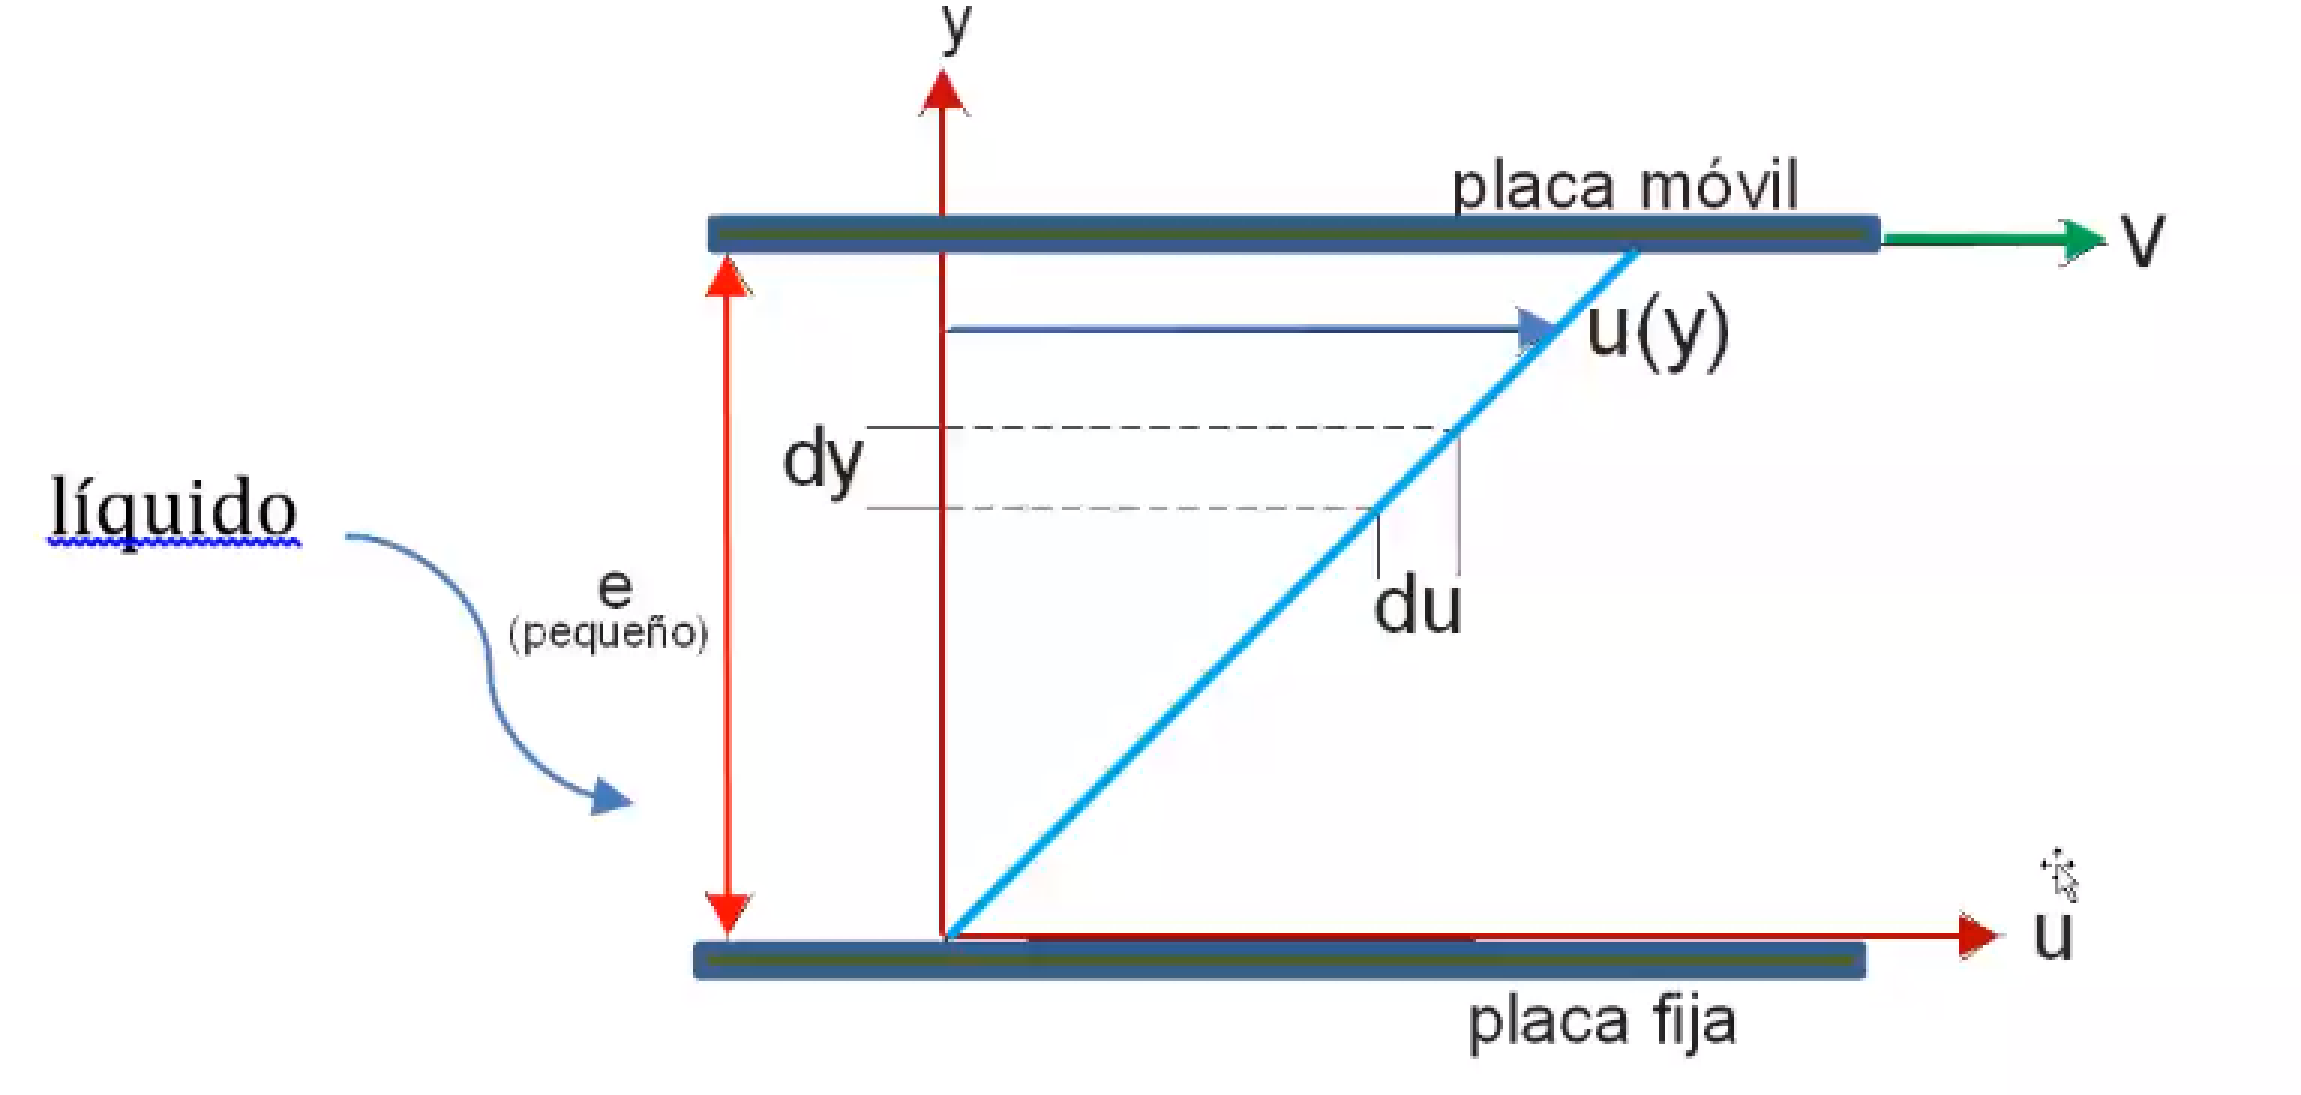
\includegraphics[width=0.5\textwidth]{hb1.png}}
  \caption{Placa móvil y placa fija}
  \label{hb1}
\end{figure}



\begin{figure}[h!]
    \centerline{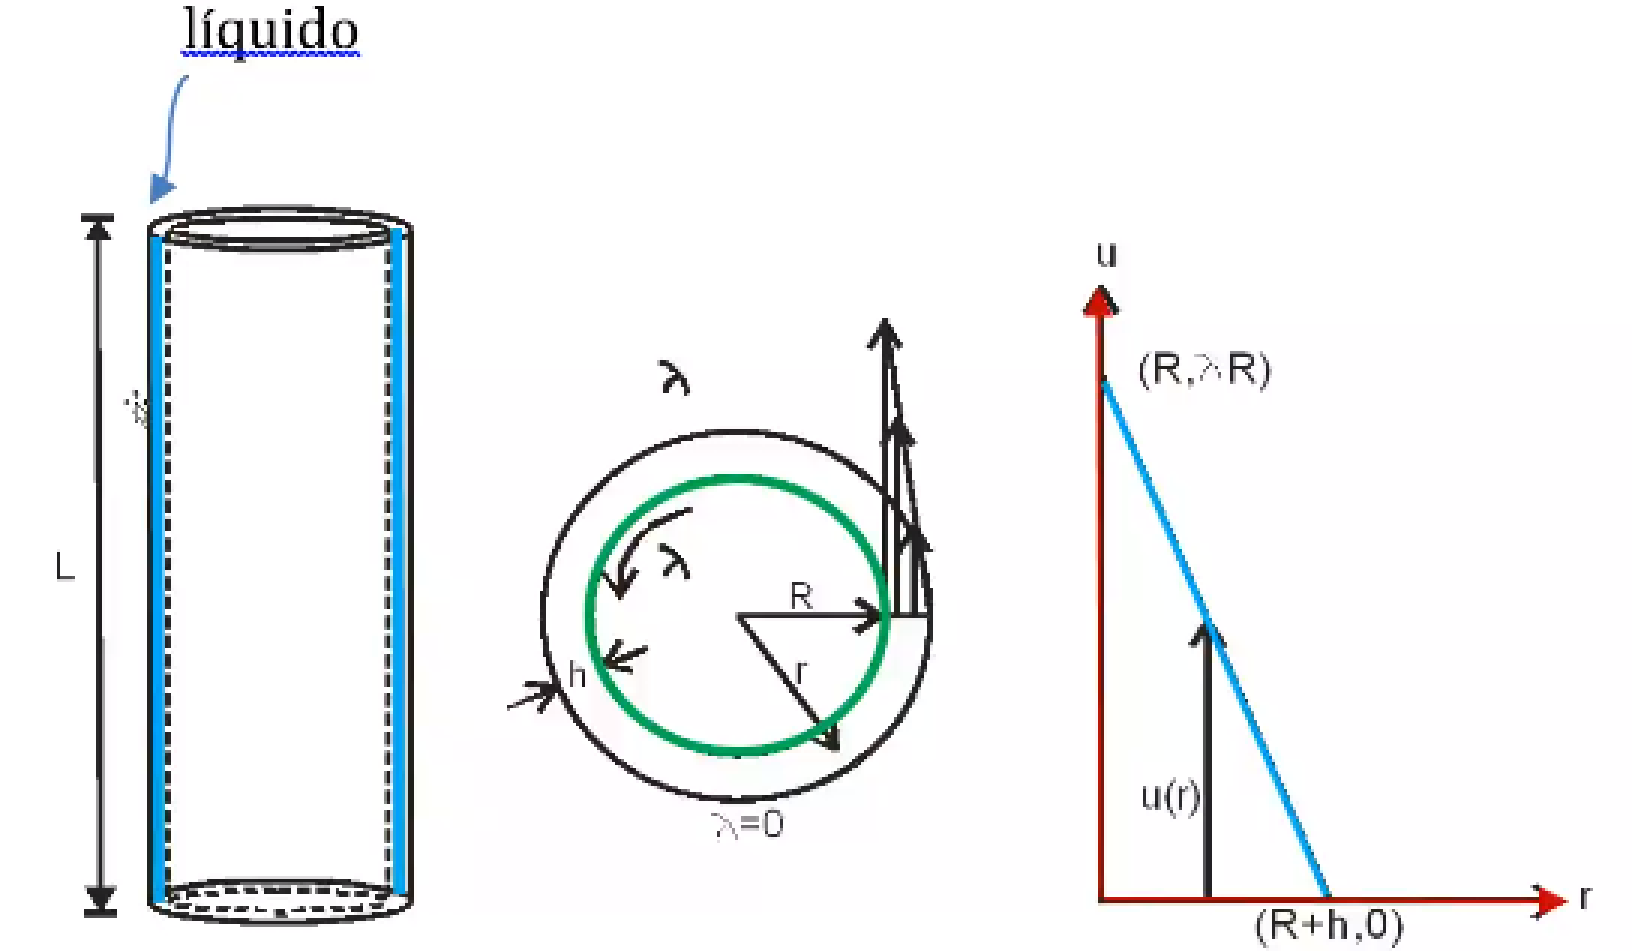
\includegraphics[width=0.5\textwidth]{hb2.png}}
    \caption{Fluido sometido a esfuerzo cortante entre dos cilindros}
    \label{hb2}
\end{figure}

\begin{equation}
    \tau=\mu\left\lvert \frac{du}{dx}\right\rvert 
\end{equation}

Donde $du/dr$ es el gradiente de velocidad y $u$ es el componente de velocidad tangencial que solo depende de $r$. Para una pequeña abertura $h\leq \mathbb{R}$, éste gradiente puede ser representado de manera aproximada suponiendo una distribución de velocidad lineal.
\begin{align}
    &\left\lvert \frac{du}{dr}\right\rvert =\frac{\lambda R}{h}&& \tau=\frac{F}{A\, contacto}&& T=D\cdot d
\end{align}

Donde $h$ es el ancho de la abertura y $\lambda$ es la velocidad angular $\left(\frac{2\pi N}{60}rad/s\right)$

Por lo tanto se puede relacionar el par de torsión aplicado $T$ con la viscosidad y los demás parámetros mediante la ecuación:
\begin{align}
    T=\mu \left\lvert \frac{du}{dr}\right\rvert 2\pi RLR=\mu\frac{\lambda R}{h}&& \tau=\frac{F}{h}2\pi RLR=\frac{2\pi R^2L\lambda \mu}{h}
\end{align}

Donde L es la longitud del cilindro rotatorio, T el esfuerzo, X el área, brazo de palanca es $\tau$. Obsérvese que el par de torsión depende directamente de la viscosidad, de éste modo los cilindros podrían utilizarse como viscosímetro, un dispositivo que mide la viscosidad de un fluido.

\begin{equation}
    \mu=\frac{Th}{2\pi L\lambda R^3}=\frac{60Th}{4\pi^2LNR^3}
\end{equation}

\subsubsection{Viscosidad cinemática}

\begin{definition}[Viscosidad cinemática]
    Es la relación entre la viscosidad dinámica del fluido y su densidad:
    \begin{equation}
        v=\frac{\mu}{\rho}=\frac{\left[FL^2T\right]}{\left[FL^4T^2\right]}=\left[L^2T\right]
    \end{equation}
    Las unidades en el sistema MKS son en $m^2/s$
\end{definition}

\begin{problem}[Se tiene un viscosímetro]
    con dos cilindros concéntricos de 30 cm de largo, uno de 20 cm de diámetro y otro de 20.2 cm de diámetro. Se requiere un par de torsión de $0.13N\cdot m$ para hacer girar el cilindro interno a 400 rpm. El líquido en el interior es agua a $2.3^{\circ}C$ Calcule la viscosidad
\end{problem}

\textit{ Sol. }

El radio es $\frac{D}{2}=10cm$. la abertura $h=\frac{20.2-20}{2}=0.1cm$
la velocidad angular es:
\begin{align*}
    &\lambda=\frac{2\pi\cdot N}{60}=\frac{2\pi\cdot 400}{60}=41.888\, rad/s\\
    &T=0.13N\cdot m=0.01325\, kg\cdot m\\
    &\mu=\frac{Th}{2\pi R^3\lambda L}=\frac{(0.01325kgm)(0.001m)}{2\pi(0.1m)^4(41.888rad/s)(0.3m)}=1.678\times 10^{-4}\frac{kg\cdot s}{m^2}\\
    &\mu=\frac{60Th}{4\pi^2 LNR^3}=\frac{60(0.01325kg\cdot m)(0.001m)}{4\pi^2(0.3m)(400rpm)(0.1m)^3}=1.6456\times 10^{-6}m^2/s\\
    &v=\frac{\mu}{\rho}=\frac{1.678\times 10^{-4}kgs/m^2}{101.967kgs^2/m^4}=1.6456\times 10^{-6}\, m^2/s
\end{align*}

\begin{table}[h!]
    \centering\begin{tabular}{@{}cc@{}}
    \toprule
    $T^{\circ}C$ & $\omega (\frac{kg}{m^3})$ \\ \midrule
    0            & 999.9             \\
    4            & 1,000.0            \\ \bottomrule
    \end{tabular}
    \caption{La densidad del agua a $2.3^{\circ}C$ se obtiene a partir de la interpolación del peso específico entre los 0 y $4^{\circ}C$}
    \label{tabhb2}
\end{table}

Se realiza una regla de tres:
\begin{align*}
    &4\longrightarrow &0.1\\
    &2.3\longrightarrow &x
\end{align*}
\begin{equation*}
    \therefore x=2.3\cdot \frac{0.1}{4}=0.0575
\end{equation*}
Así $\omega$ para $2.3^{\circ}C$ es 999.9+0.0575=999.9575 $\frac{kg}{m^3}$
y la densidad será $\frac{\omega}{g}=\frac{999.9575\frac{kg}{m^3}}{9.80665\frac{m}{s^2}}=101.967kg\cdot s^2/m^4$


\begin{problem}[Un líquido con viscosidad]
    de $1.5\times 10^{-3} kg\cdot s/m^2$ fluye sobre una superficie horizontal. Calcular el gradiente de velocidades y la intensidad del esfuerzo cortante en la frontera  a punto situados a 1.2 y 3 cm desde la misma suponiendo:
    \begin{itemize}
        \item Distribución lineal de velocidades
        \item Distribución parabólica de velocidades. La parábola tiene su vértice en A y el origen en B
    \end{itemize}
\end{problem}

\begin{figure}[h!]
    \centerline{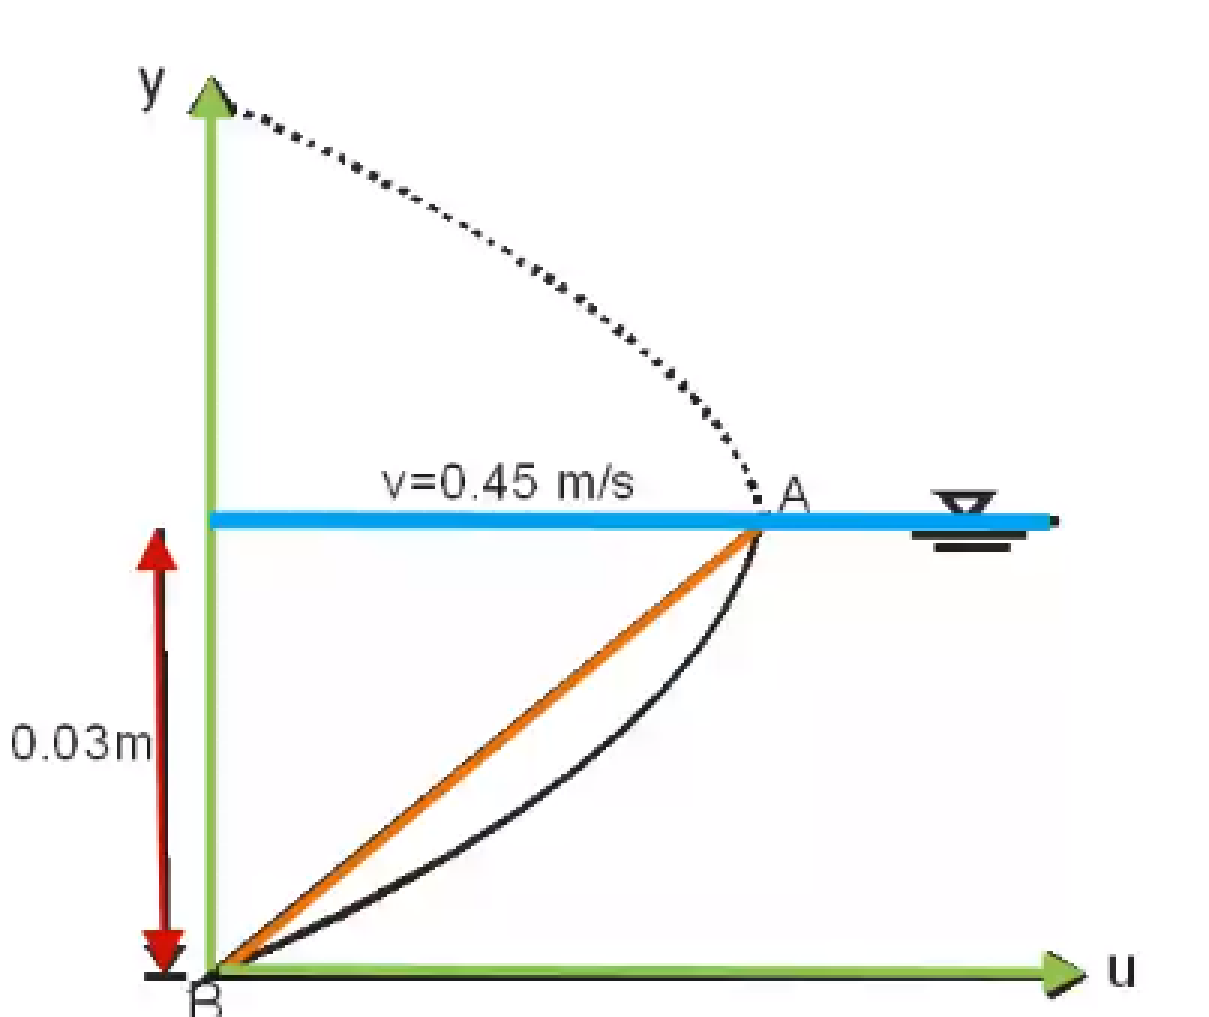
\includegraphics[width=0.5\textwidth]{hb3.png}}
    \caption{Esquema del problema}
    \label{hb3}
  \end{figure}

\textit{ Sol. }

\begin{enumerate}
    \item Para la distribución lineal de velocidades, la relación entre la viscosidad y la distancia es desconocida, el gradiente de velocidades es: $\frac{dv}{dy}=15s^{-1}$ entonces el esfuerzo cortante vale:

    \begin{equation*}
        \tau=\mu\cdot \frac{dv}{dy}=\left(0.0015kg\cdot s/m^2\right)\left(15s^{-1}\right)=0.0225kg/m^2
    \end{equation*}
    
    el cual es constante para el resto de los puntos ya que $\frac{dv}{dy}$ no depende de $y$
    \item La ecuación de la parábola debe satisfacer la condición de que la velocidad sea cero en el punto B sobre la frontera, se puede obtener mediante álgebra dicha ecuación es sistema MKS.

    \begin{equation*}
        v=30y-500y^2
    \end{equation*}
    Por lo que el gradiente de velocidad será:
    
    \begin{equation*}
        \frac{dv}{dt}=30-1,000y
    \end{equation*}
    Así el esfuerzo será función de $y$
    \begin{equation*}
        \tau-\mu\frac{dv}{dy}\mu\left(30-1,000y\right)
    \end{equation*}
    
    \begin{table}[h!]
        \centering
        \begin{tabular}{@{}cccc@{}}
        \toprule
        y(m) & v(m/s) & $\frac{dv}{dy}s^{-1}$ & $\tau$ $kg/m^2$ \\ \midrule
        0.00 & 0.00   & 30                    & 0.045           \\
        0.01 & 0.25   & 20                    & 0.030           \\
        0.02 & 0.40   & 10                    & 0.015           \\
        0.03 & 0.45   & 0                     & 0.000           \\ \bottomrule
        \end{tabular}
        \caption{Resultados del esfuerzo}
        \label{tabhb3}
        \end{table}
    
\end{enumerate}

\subsubsection{Tensión superficial}

\begin{figure}[h!]
  \centerline{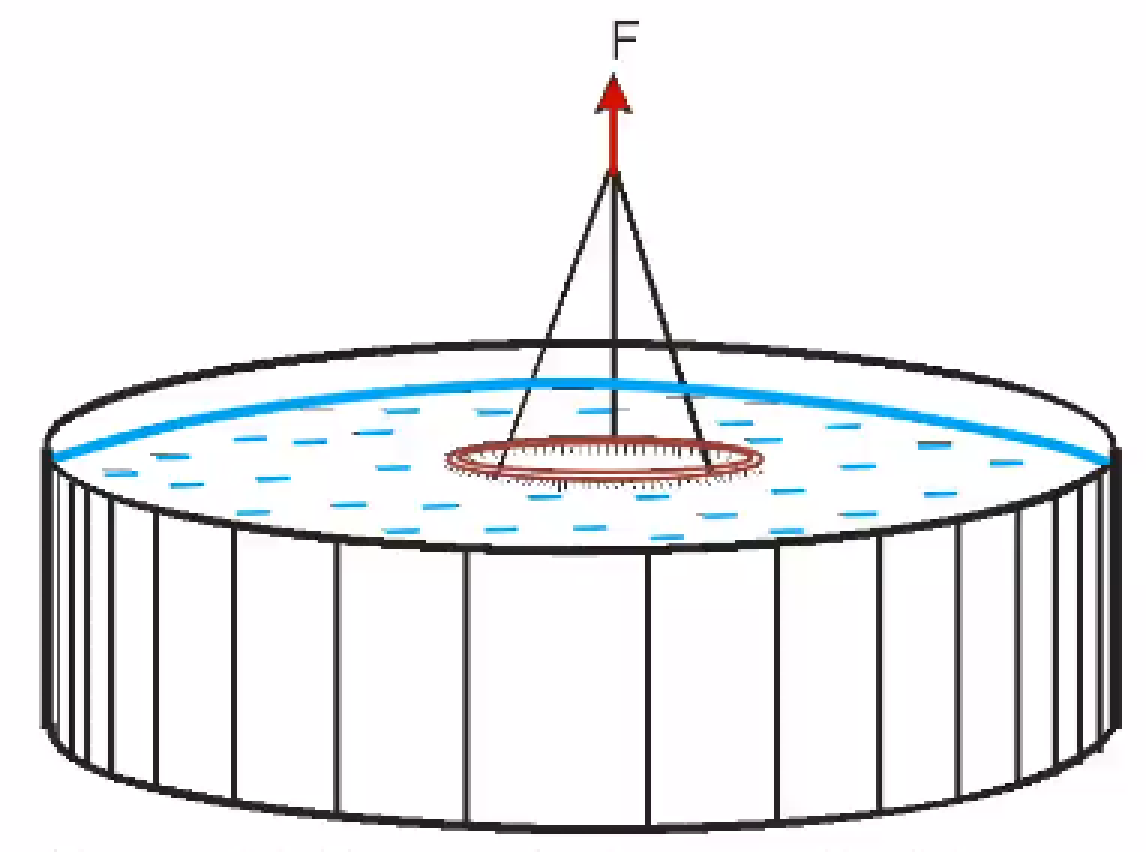
\includegraphics[width=0.5\textwidth]{hb4.png}}
  \caption{Extracción de un anillo del interior de un líquido}
  \label{hb4}
\end{figure}

De la figura \ref{hb4}, $F:$ es la fuerza para extraer el anillo, $W$ es el peso de anillo y cuerda, $F_{\sigma}$ la fuerza de tensión superficial. De aquí se deduce

\begin{equation}
    F=W+F_{\sigma}=W+2\pi\cdot D\cdot \sigma
\end{equation}

donde $\sigma=\frac{F-W}{2\pi D}$

\begin{problem}[Para extraer horizontalmente un anillo de cobre de un líquido se requiere $1/2N$]
    Determine la tensión superficial del líquido. (peso del hilo: $2g$). $s_{Cu}=8.9$
\end{problem}

\textit{ Sol. }
\begin{align*}
    &D_{alambre}=3mm&&D_{a}=20cm
\end{align*}
\begin{align*}
    &W=\pi\cdot D_{a}\left(\pi\cdot \frac{D^2_{at}}{4}\right)\omega_{Cu}+2g\\
    &\pi(0.2m)\left(\pi\cdot \frac{0.003^2}{4}\right)8900+0.002kg=0.04153\\
    &F=0.5N=0.05097kg\\
    &\sigma=\frac{0.05097kg-0.04153kg}{2\pi(0.2)}=7.51\times 10^{-3}kg/m\\
    &\sigma=7.51\times 10^{-3}kg/m\left(\frac{9.81N}{1kg}\right)=7.367\times 10^{-2}N/m
\end{align*}

\subsubsection{Capilaridad}

\begin{definition}[Capilaridad]
    Es la acción (elevación o descenso) de un líquido en  un tubo capilar (o en situaciones físicas análogas tales como en medios porosos), provocada por la tensión superficial y originada en la relación que presenta la adhesión entre líquido y sólido con la cohesión del líquido. Los líquidos ascienden en tubos que mojan (adhesión > cohesión) y el menisco que se forma será cóncavo, y descienden en tubos a los que no mojan, (cohesión > adhesión) en cuyo caso el menisco es convexo
\end{definition}

La relación que existe entre algunas propiedades físicas de los líquidos que se muestra a continuación: 

Para caso de $F_{adherencia} > F_{cohesion}$: Mientras el peso de la columna es menor que las fuerzas capilares en la vertical, estará ascendiendo el líquido hasta que alcanza el equilibrio

\begin{figure}[h!]
  \centerline{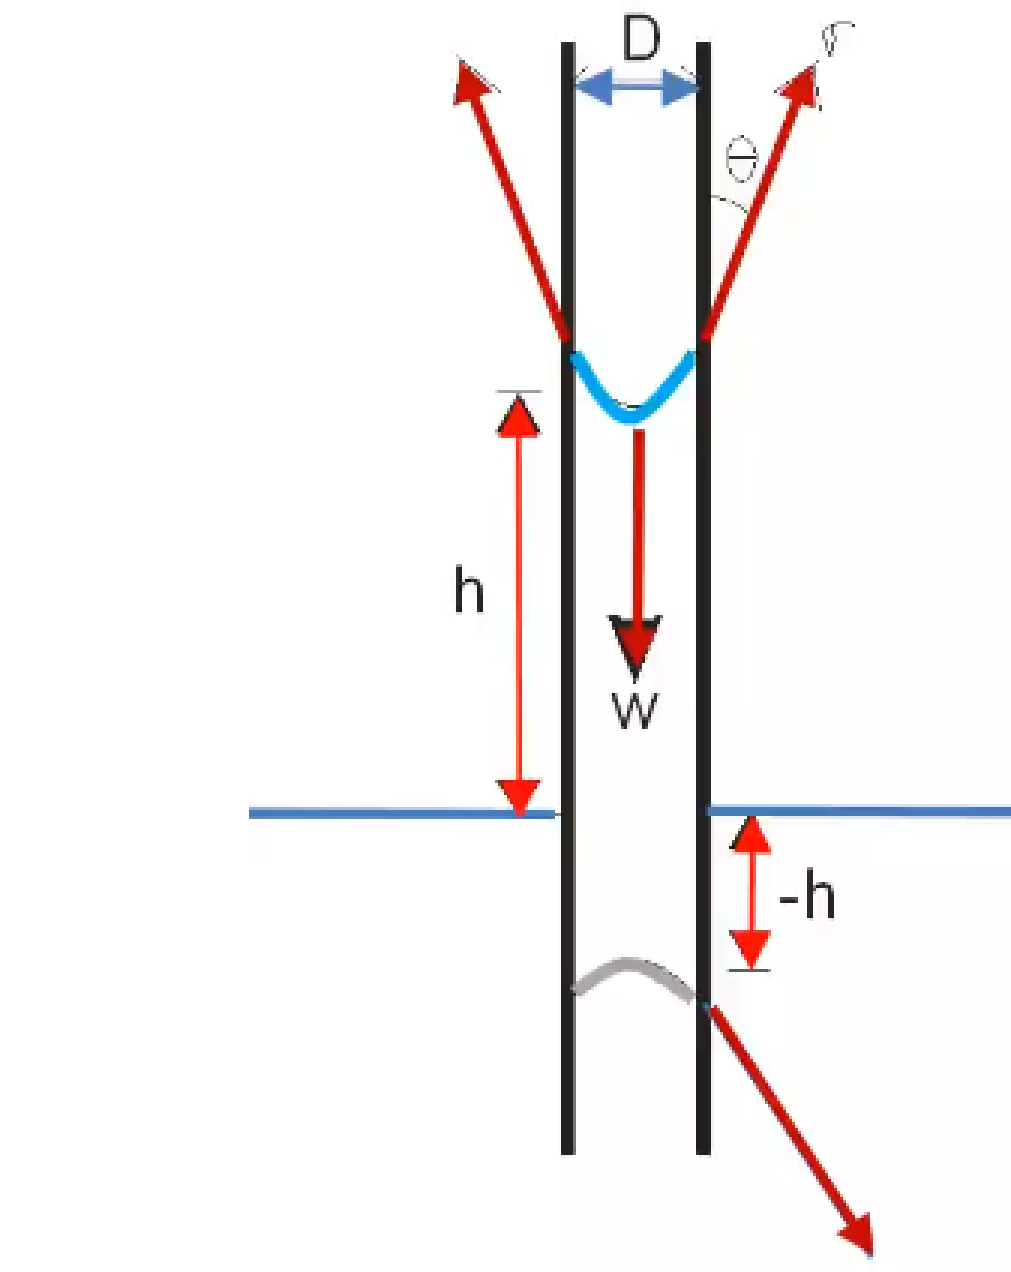
\includegraphics[width=0.5\textwidth]{hb5.png}}
  \caption{Fuerza de adherencia y Cohesión}
  \label{hb5}
\end{figure}

\begin{equation}
    \frac{\pi D^2}{4}h\omega=\sigma\cos{(\theta)}\pi D
\end{equation}
\begin{equation}
    h=\frac{4\sigma\cos{(\theta)}}{D\omega}
\end{equation}

Para caso de $F_{coehesion} > F_{adherencia}$. un caso de descenso capilar $(-h)$ ocurre en mercurio en donde $\theta>90$ y $\cos{(\theta)}$ es negativo

\begin{problem}[Se inserta un tubo de vidrio limpio]
    de 2mm de diámetro en agua a $15^{\circ}C$. Determine la altura a la que sube el agua en el tubo. El agua forma un ángulo de contacto (prácticamente de $0^{\circ}$ con el vidrio limpio)
\end{problem}
\textit{ Sol. }

\begin{equation*}
    h=\frac{4\sigma\cos{(\theta)}}{D\omega}=\frac{4(7.5\times 10^{3}kg\cdot m)\cos{(0)}}{(0.002m)(998.95\frac{kg}{m^3})}=0.015016m
\end{equation*}

Determine el ascenso capilar de ahí a $20^{\circ}C$ en limo (2-60 micras) y en arena (60 micras a 2 mm).
Considere $Dporo=Dpart/10$.

\begin{table}[h!]
    \centering\begin{tabular}{@{}ll@{}}
    \toprule
    \multicolumn{2}{l}{Altura capilar en materiales} \\ \midrule
    Material              & Altura cap. (m)          \\
    Arena Gruesa          & 0.12-0.18                \\
    Arena Fina            & 0.30-1.20                \\
    Limo                  & 0.76-7.60                \\
    Arcilla               & 7.60-23.0                \\ \bottomrule
    \end{tabular}
    \caption{DAS (1998)}
    \label{tabhb4}
\end{table}
\begin{align*}
    &h=\frac{4\sigma\cos{(\theta)}}{D\omega}=\frac{4(7.5\times 10^{3}kg\cdot m)\cos{(0)}}{(0.002m)(998.95\frac{kg}{m^3})}=0.015016m\\
    &h=\frac{4\sigma\cos{(\theta)}}{D\omega}=\frac{4(7.5\times 10^{3}kg\cdot m)\cos{(0)}}{(0.002m)(998.95\frac{kg}{m^3})}=0.015016m
\end{align*}

%HISTÉRESIS
\subsubsection{Compresibilidad}
La compresibilidad es la propiedad que tienen los cuerpos de variar su volumen bajo la acción de variación de presiones externas. Des esta definición se deriva el concepto de módulo de elasticidad volumétrica $(E)$ de los líquidos y se define como el cambio de intensidad de presión $(\Delta p)$, dividido por el cambio correspondiente del volumen $(\Delta V)$ por unidad de volumen como se indica en la fórmula

\begin{figure}[h!]
  \centerline{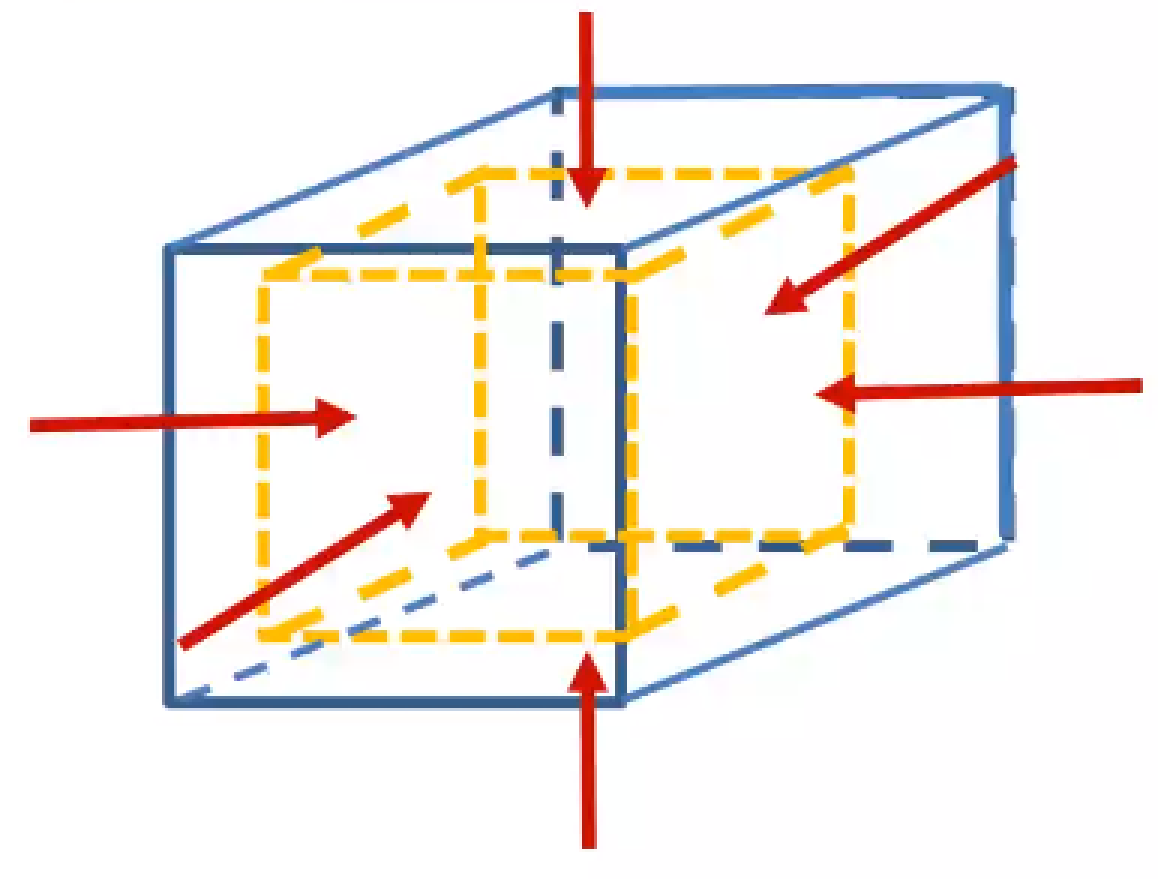
\includegraphics[width=0.5\textwidth]{hb6.png}}
  \caption{Compresibilidad de un líquido}
  \label{hb6}
\end{figure}

\begin{equation}
    -\Delta V=V_2-V_1
\end{equation}

Si se aumenta la presión $p_2> p_1$ entonces $\Delta =p_2-P-10$

\begin{equation}
    E=-\frac{V\Delta p}{\Delta}
\end{equation}

El valor de $E$ varía principalmente con la temperatura, para el agua se tiene una variación de $20600\frac{kg}{cm^2}$ a $0^{\circ}C$. Estos valores son lo suficientemente elevados para permitir el supuesto de que el agua es incompresible en resolución de la mayoría de los problemas de hidráulica

\begin{example}
    En el océano, la presión a 8km de profundidad es de $1050\frac{kg}{cm^2}$, el peso específico en la superficie es $1025\frac{kg}{m^3}$ y el módulo de elasticidad promedio es $23,000\frac{kg}{cm^2}$ para este intervalo de presiones. Calcular el volumen y el peso específico a esa profundidad
\end{example}

\textit{ Sol. }

Partiendo de la expresión de módulo de elasticidad: 

\begin{equation*}
    \Delta V=-\frac{V\Delta p}{E}=-\frac{1m^3\cdot 1050\frac{kg}{cm^2}}{23,000\frac{kg}{cm^2}}=-0.0565m^3
\end{equation*}
Lo que significa una variación de $(-0.0565m^3/1m^3)\cdot 100=-4.565$\%

Esto es que $1m^3$ en la superficie pesa 1025 kg, a 8 km de profundidad $(1-0.04565)=0.95435m^3$
siguen pesando 1025 kg. Así el peso específico será: 

\begin{equation*}
    \omega^{\prime}=\frac{1025kg}{0.95435}=1074kg(m^3)
\end{equation*}

\begin{problem}
    Determine la variación de volumen en \% de peso específico y de densidad del agua al pasar de cero a una presión en el sistema gravitacional y absoluto.
    \begin{enumerate}
        \item 60 m en el fondo de una cortina en una presa a $15^{\circ}C$
        \item 235 m en el interior de una tubería a $32^{\circ}C$
    \end{enumerate}
\end{problem}

\textit{ Sol. }
\begin{align*}
    &\Delta V=-0.000275m^3&&dif(\%)=-0.0275\%&&\omega=999.225\frac{kg}{m^3}=&&9802.397N/m^3\\
    &\rho=101.858utm/m^3&&=999.225kg_m^4m^3
\end{align*}
\begin{align*}
    &\Delta V=-0.000102m^3&&dif(\%)=-0.102\%&&\omega=996.01\frac{kg}{m^3}=9770.86N/m^3\\
    &\rho=101.53kg\cdot s/m^4&&=996.01kg_m/m^3
\end{align*}

\section{Hidrostática}

La hidrostática es la rama de la hidráulica que se encarga del estudio de los líquidos en estado de reposo relativo, esto es que sus partículas no presentan movimiento relativo entre ellas. Si no hay movimiento relativo, no existen esfuerzos cortantes, puesto que para ellos se requieren gradientes de velocidad. El único esfuerzo que existe es un esfuerzo normal, la presión
por lo que esta es de primordial importancia en la hidrostática. La única presión que generan los líquidos en reposo es la llamada presión hidrostática.

La presión hidrostática es la fuerza por unidad de área que ejerce un líquido en reposo sobre una superficie real o imaginaria situada dentro o en periferia.

Algunas aplicaciones de la presión hidrostática es en el diseño de dispositivos y objetivos sumergidos, tales como presas, tuberías, válvulas, tanques de almacenamiento, superficies de barcos, prensas hidráulicas, gatos hidráulicos, frenos, transmisores y direcciones hidráulicas.

Clasificación de presión $(FL^{-2})$

La presión se clasifica en: 

\begin{enumerate}
    \item \textbf{Absoluta} Cuando se toma en cuenta la presión atmosférica (a partir del vacío o cero absoluto)
    \item \textbf{Relativa} Cuando no se toma en cuenta la presión atmosférica, también llamada hidrostática o manométrica
    \item \textbf{Unitaria} Cuando su intensidad se refiere a la unidad de área
    \item \textbf{Total} Cuando se refiere a toda una superficie y corresponde a la intensidad de empuje hidrostático
\end{enumerate}

\begin{figure}[h!]
  \centerline{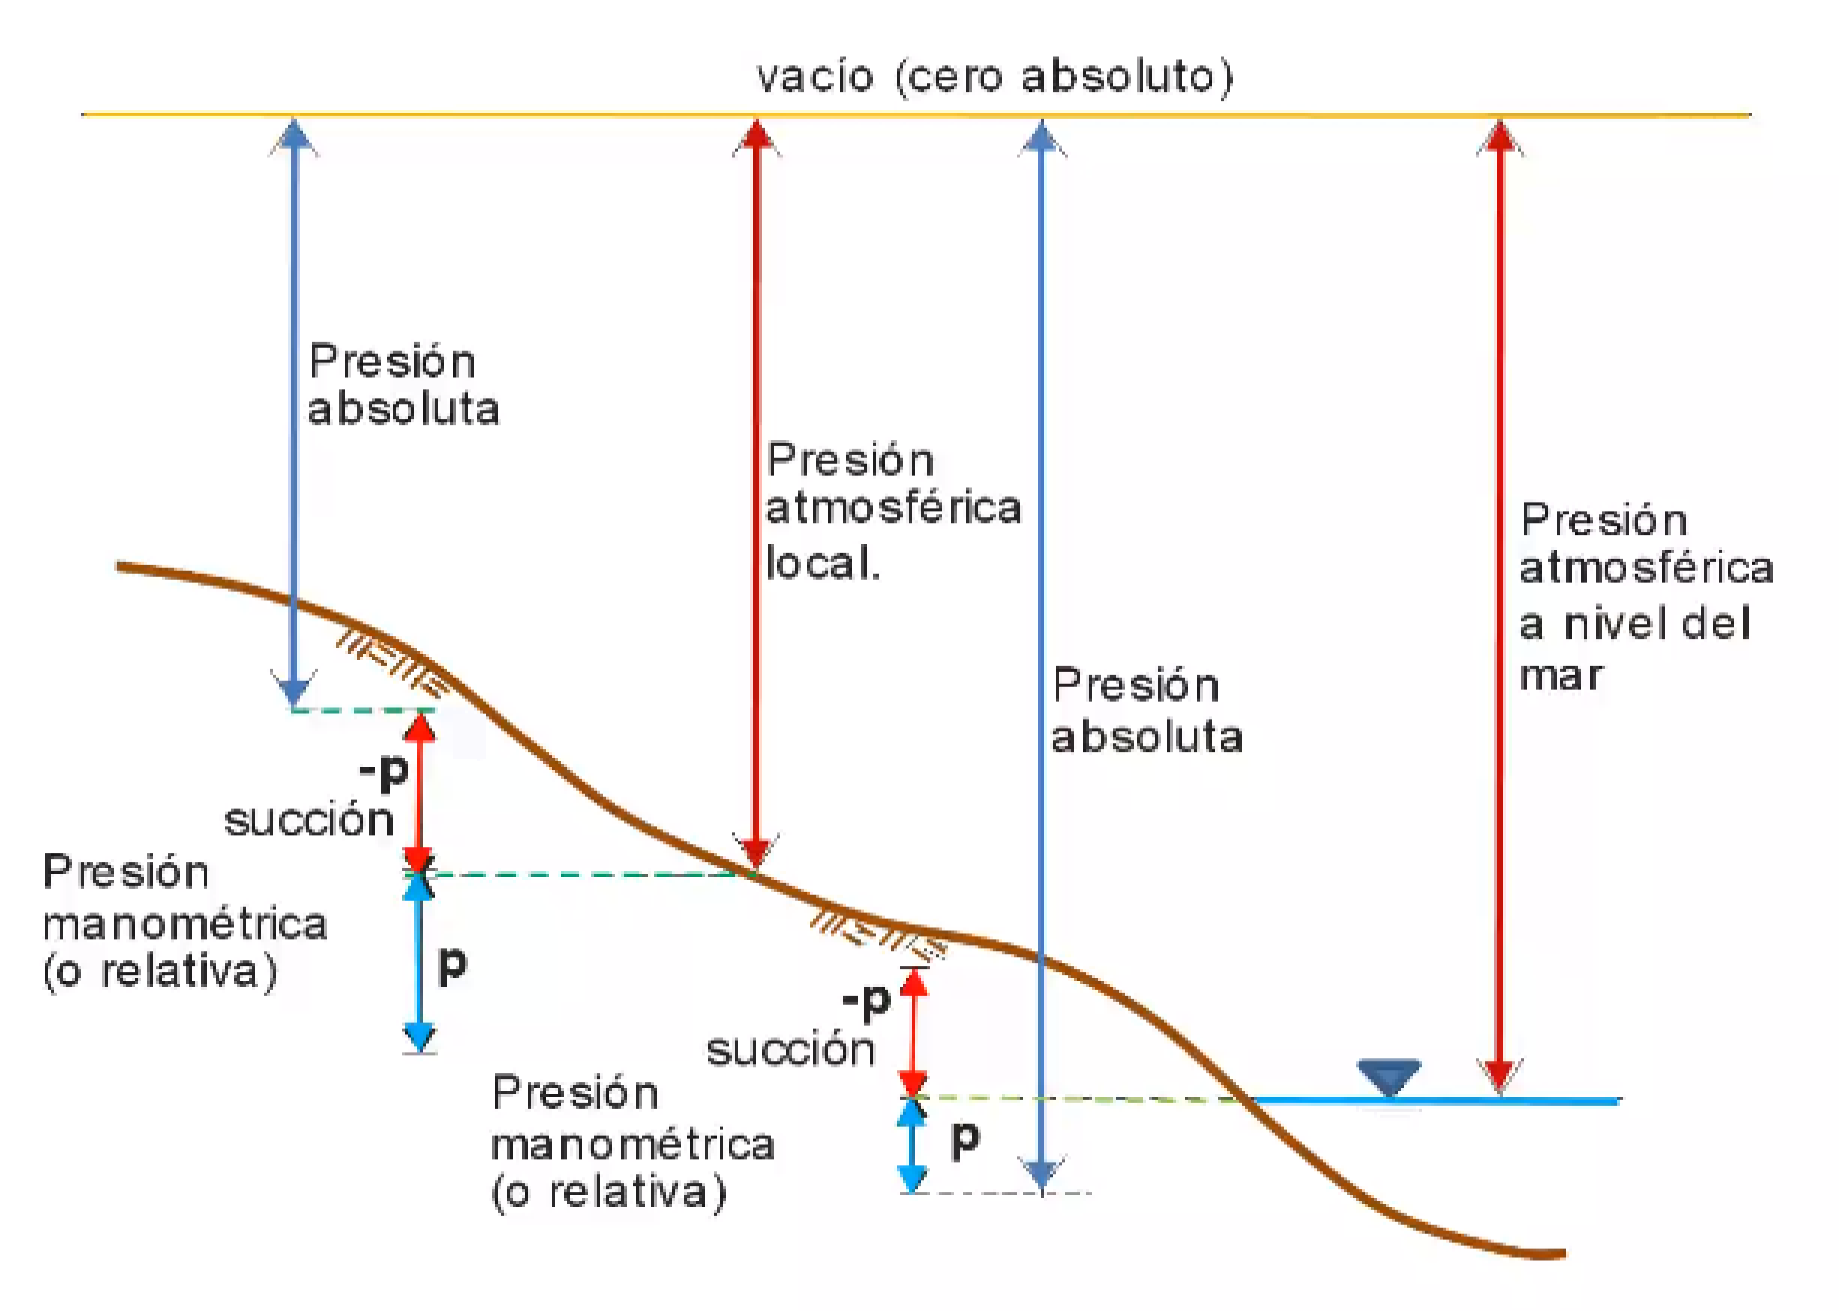
\includegraphics[width=0.5\textwidth]{hb7.png}}
  \caption{Efectos de la presión sobre la superficie terrestre}
  \label{hb7}
\end{figure}

\subsection{Ecuaciones fundamentales de la hidrostática}

Una característica fundamental de cualquier fluido en reposo es que la fuerza ejercida sobre cualquier partícula del fluido es la misma en todas direcciones.

Aplicando la segunda ley de Newton al elemento, en las direcciones $x$ y $y$

\begin{figure}[h!]
  \centerline{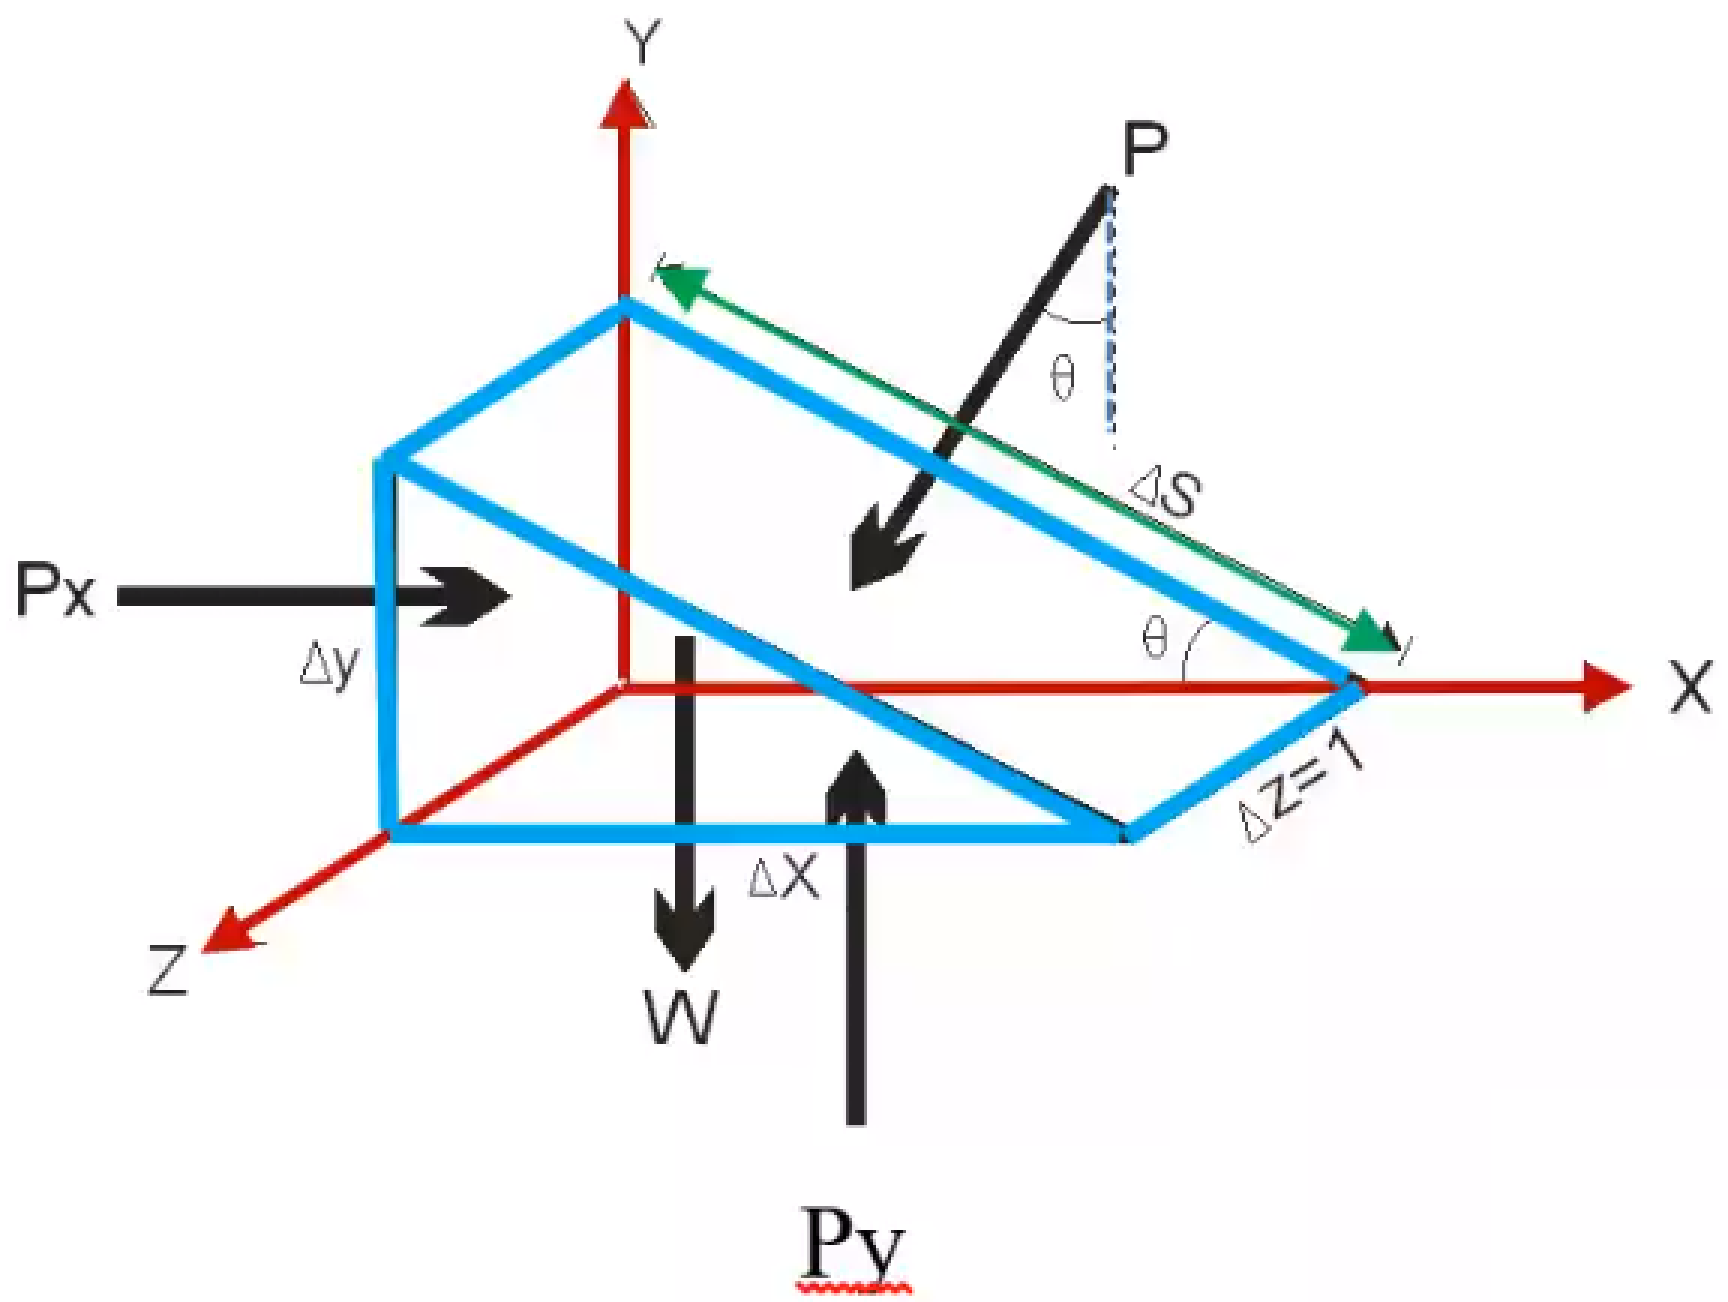
\includegraphics[width=0.5\textwidth]{hb8.png}}
  \caption{Demostración del teorema de Pascal}
  \label{hb8}
\end{figure}
\begin{align*}
    &\sum F_x=ma_x\\
    &p_x\Delta y-p\Delta s\cdot \sin{(\theta)}=p\frac{\Delta x\Delta y}{2}a_x\\
    &\sum F_y=ma_y\\
    &p_y\Delta x-pg\frac{\Delta x \Delta y}{2}-p\Delta s\cdot \cos{(\theta)}=p\frac{\Delta x\Delta y}{2}a_y\\
    &\Delta s\cdot \sin{(\theta)}=\Delta y\quad \Delta s\cdot \cos{(\theta)}=\Delta x
\end{align*}
Las ecuaciones anteriores toman la forma:
\begin{align*}
    &p_x-p=p\frac{\Delta x}{2}a_x\\
    &p_y-p=p\frac{\Delta y}{2}a_y+pg\frac{\Delta y}{2}=p\frac{\Delta y}{2}(g+a_y)
\end{align*}

Si $\Delta x\to 0$ y $\Delta y\to 0$, el prisma se convierte en un punto $y$ girando el prisma en el plano horizontal.
\begin{equation}
    p_x=p_y=p=p_z
\end{equation}

donde se utilizó $\Delta v=\frac{\Delta x\cdot \Delta y}{2}$ se podría incluir $\Delta z$ para incluir espesor. Las presiones mostradas se deben al fluido circundante y son las presiones promedio que actúan en las áreas. Sustituyendo observe que en el límite $\Delta x\to 0$
y $\Delta y\to 0$, el elemento prismático se convierte en un punto. Por lo tanto los lados derechos de las ecuaciones anteriores, se vuelven cero, o en caso de fluidos en movimiento (sin desarrollar esfuerzos cortantes), lo que da el resultado de que en un punto: 

\begin{equation}
    p_x=p_y=p=0
\end{equation}


\begin{theorem}[Teorema principal de la hidrostáticas]
    Al teorema principal de la hidrostática se le conoce como  el de la diferencia de presiones hidrostáticas unitarias y su enunciado es la siguiente: \emph{En un líquido ideal en reposo la diferencia de presiones de dos puntos en su interior, vale la diferencia de sus respectivos tirantes por el peso volumétrico del líquido}
\end{theorem}

Para demostrar éste teorema, se plantea lo siguiente: 

\begin{figure}[h!]
  \centerline{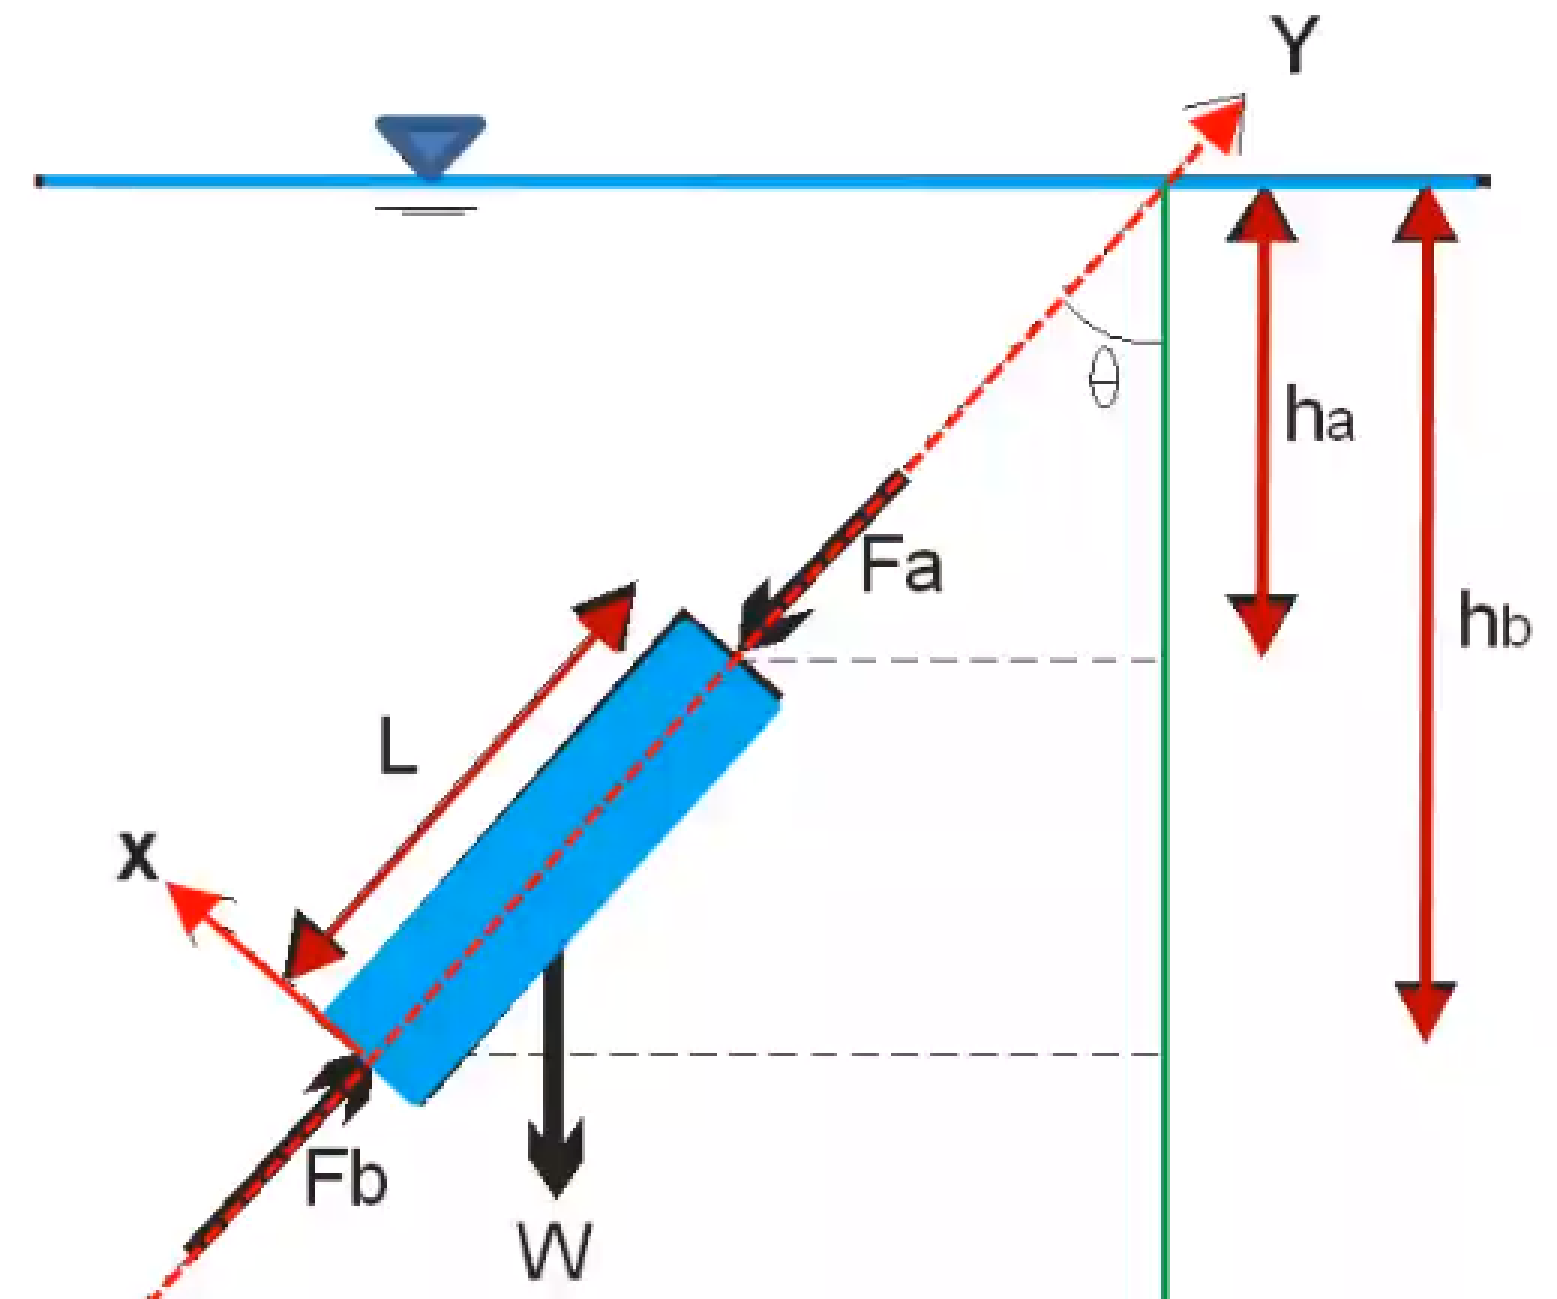
\includegraphics[width=0.5\textwidth]{hb9.png}}
  \caption{Demostración del teorema de la diferencia de presiones unitarias}
  \label{hb9}
\end{figure}

\begin{proof}[Teorema principal de la hidrostáticas]
    \begin{align*}
        &\sum F_y=0\\
        &F_b-F_a-W\cos{(\theta)}=0\\
        &\Delta x\Delta z\cdot P_b-\Delta x\Delta z\cdot P_a-\bar{w}\Delta x\Delta zL\cdot \cos{(\theta)} =0
    \end{align*}
    Eliminando a $\Delta x$ y $\Delta z$ como: $L\cos{(\theta)}=h_h-h_a$:
    \begin{equation*}
        P_b-P_a=\bar{\omega}\left(h_b-h_a\right)
    \end{equation*}
    lo que demuestra el teorema en cuestión
\end{proof}
Este teorema tiene tres corolarios (Proposición que se deduce por sí sola de lo demostrado anteriormente)

\begin{corollary}
    La magnitud de la presión unitaria (relativa) en un punto en el interior de un líquido homogéneo en reposo (relativo) vale el tirante del punto por el peso volumétrico del líquido
    \begin{equation}
        P=\omega\cdot h
    \end{equation}
\end{corollary}

\begin{corollary}
    Puntos localizados en un plano a nivel dentro de un líquido homogéneo, o ligado por un líquido homogéneo, tienen la misma presión hidrostática.
    \begin{align}
        &P_1=P_2\neq P_3\neq P_4=P_5\\ 
        &P_6\neq P_7\neq P_8
    \end{align}
\end{corollary}
\begin{figure}[h!]
  \centerline{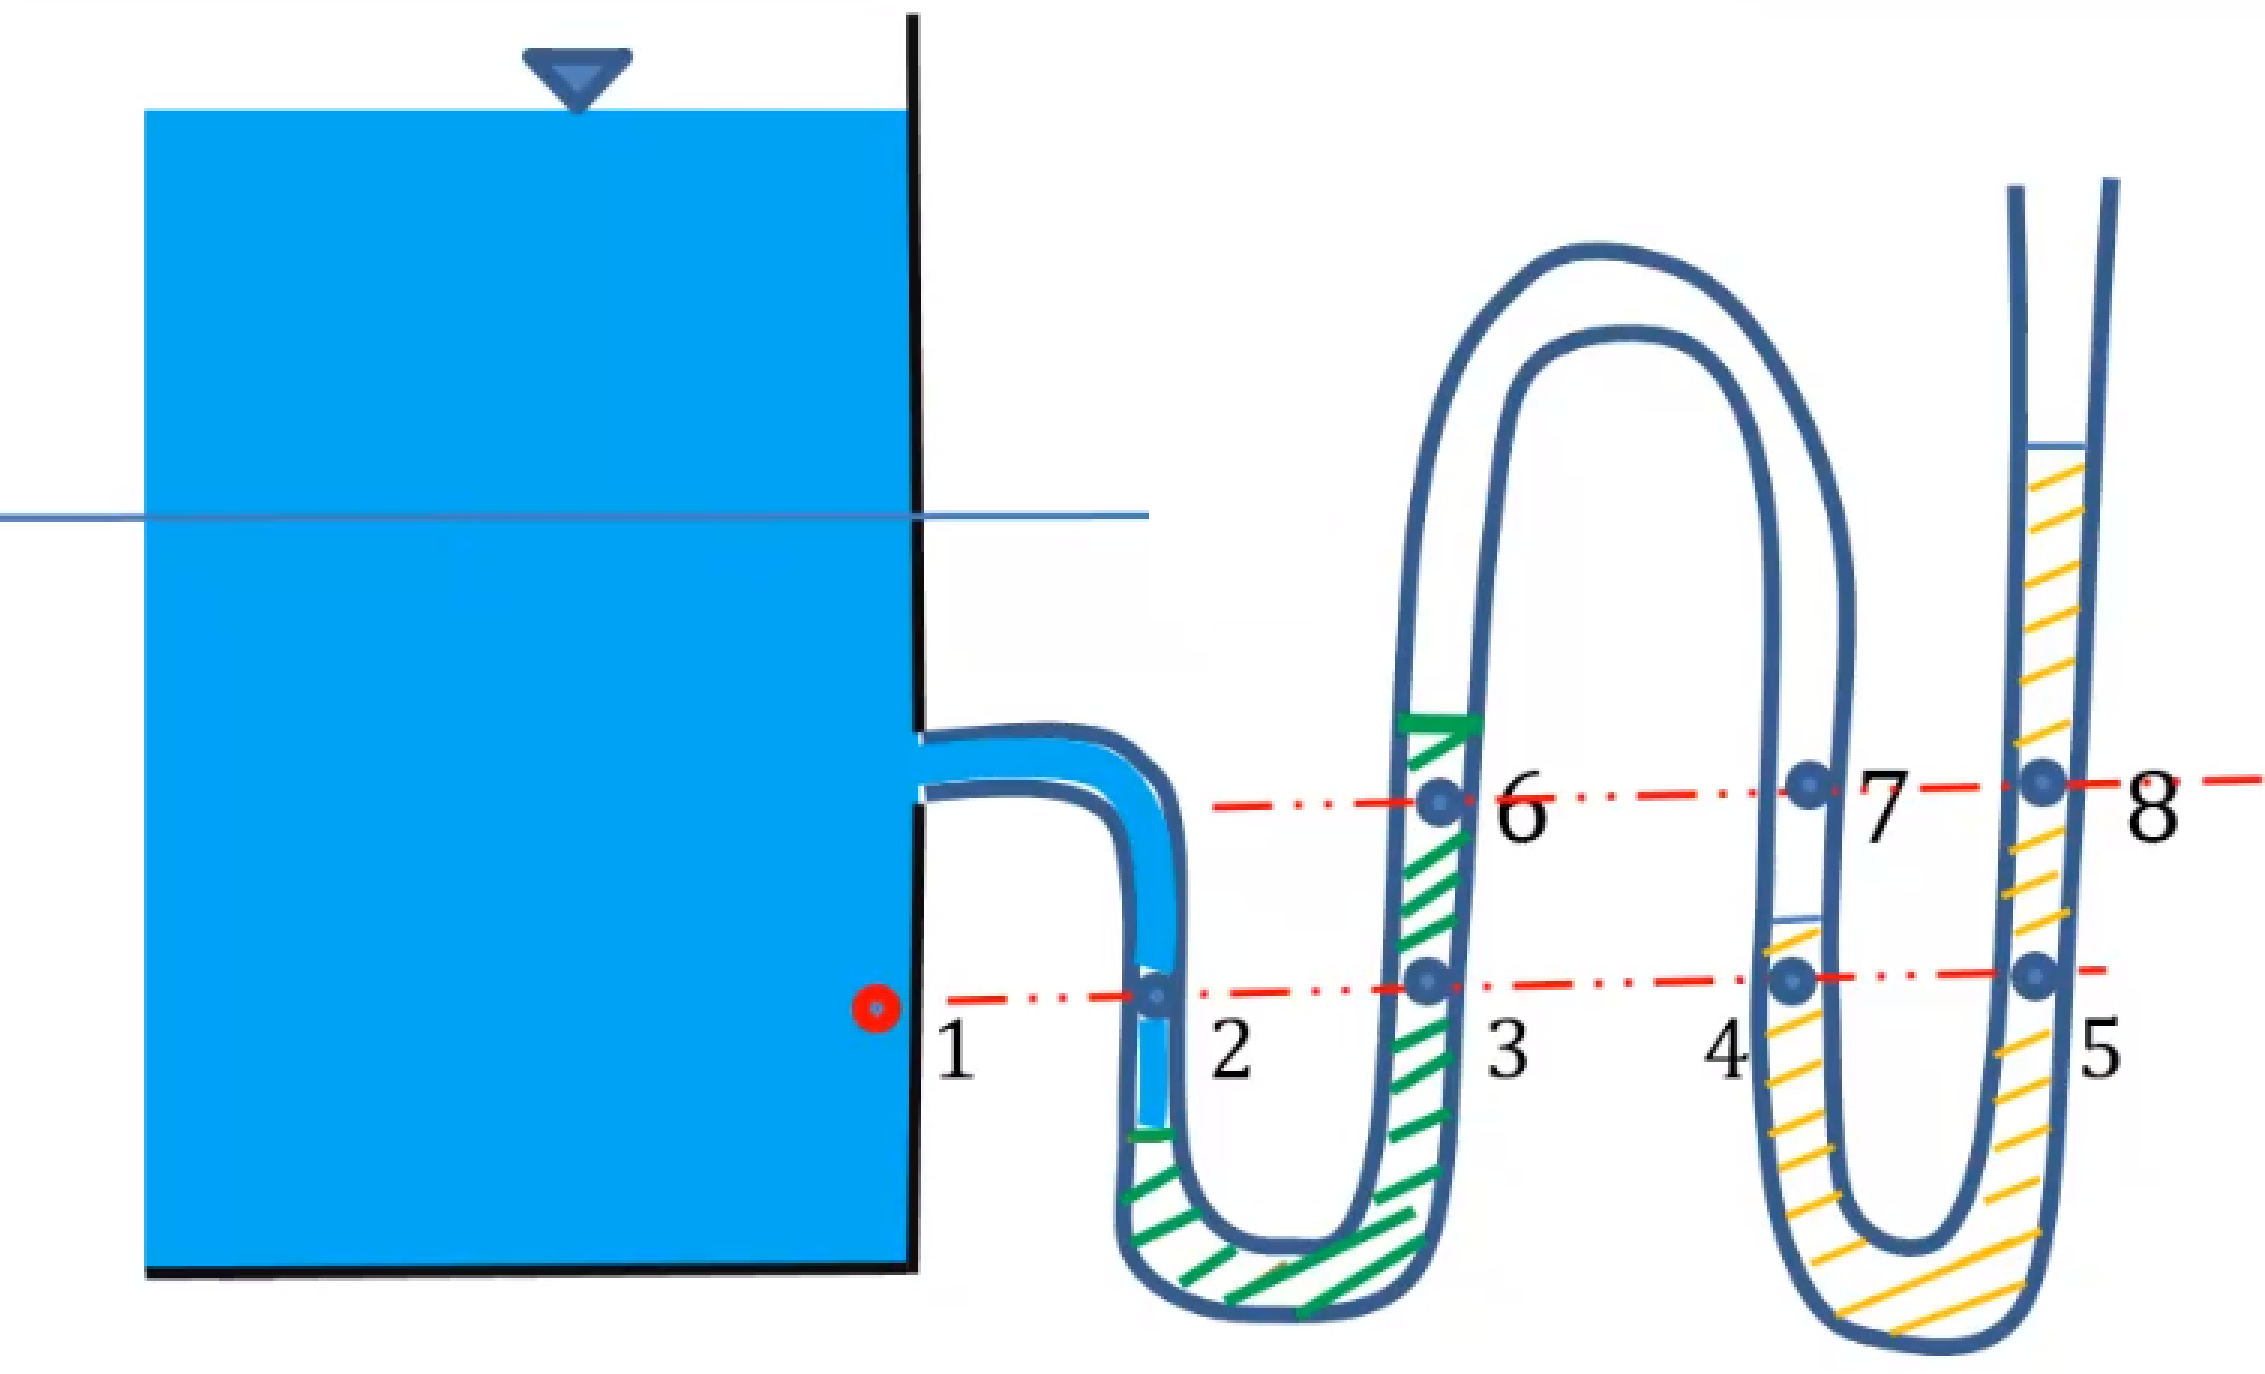
\includegraphics[width=0.5\textwidth]{hb10.png}}
  \caption{Presión hidrostática}
  \label{hb10}
\end{figure}

\begin{corollary}
    En un líquido en reposo, las presiones hidrostáticas unitarias se transmiten en todos los sentidos y direcciones con igual intensidad
\end{corollary}
\begin{figure}[h!]
  \centerline{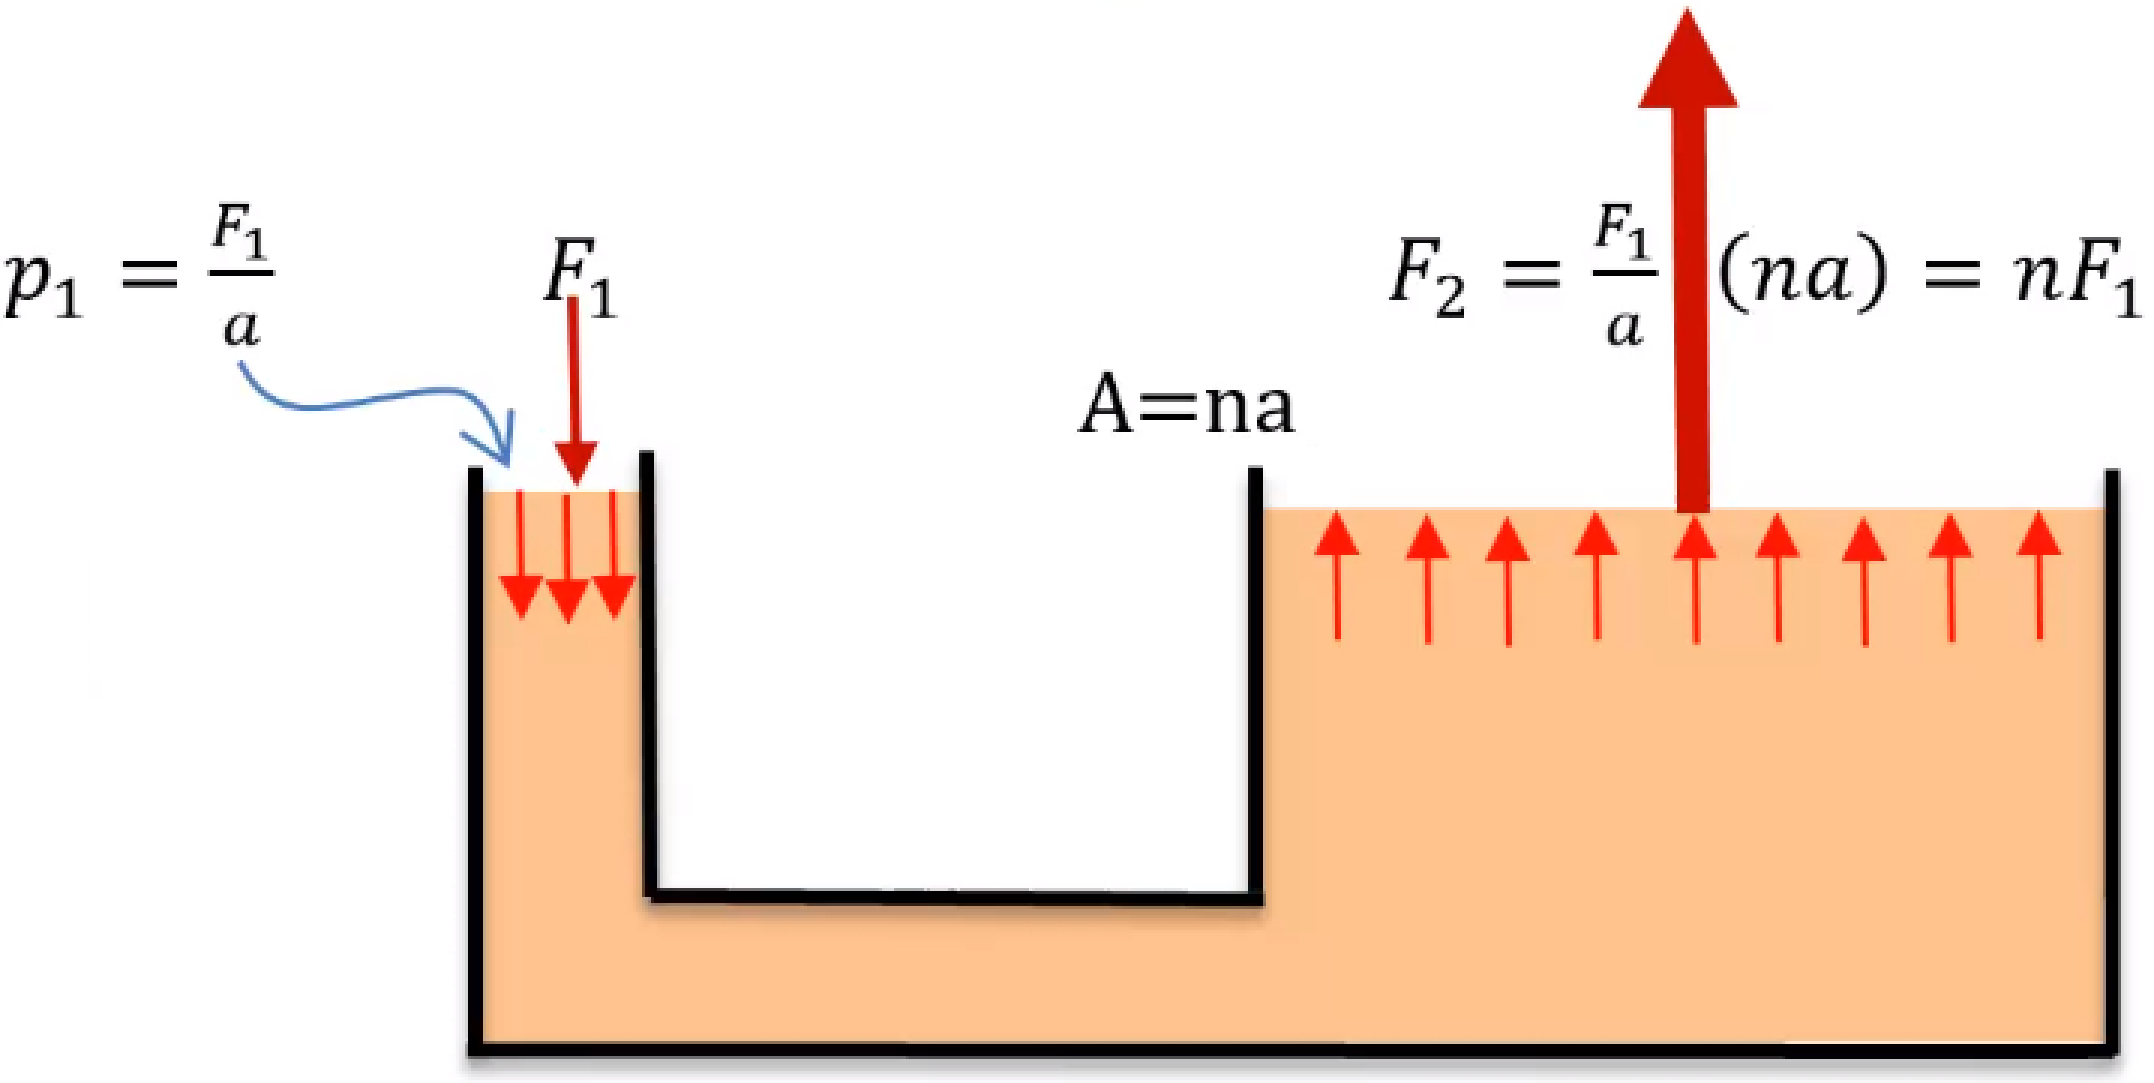
\includegraphics[width=0.5\textwidth]{hb11.png}}
  \caption{Esquema de un un principio}
  \label{hb11}
\end{figure}


\begin{example}
    ¿Cuánto vale la presión hidrostática unitaria en $d$ de la figura necesaria para calcular el espesor del cajón? Los pesos específicos de los líquidos:
    \begin{enumerate}
        \item Para mercurio $13600\frac{kg}{m^3}$
        \item Para el agua $1,000\frac{kg}{m^3}$
        \item Para el petróleo $900\frac{kg}{m^3}$
    \end{enumerate}
\end{example}

\begin{figure}[h!]
  \centerline{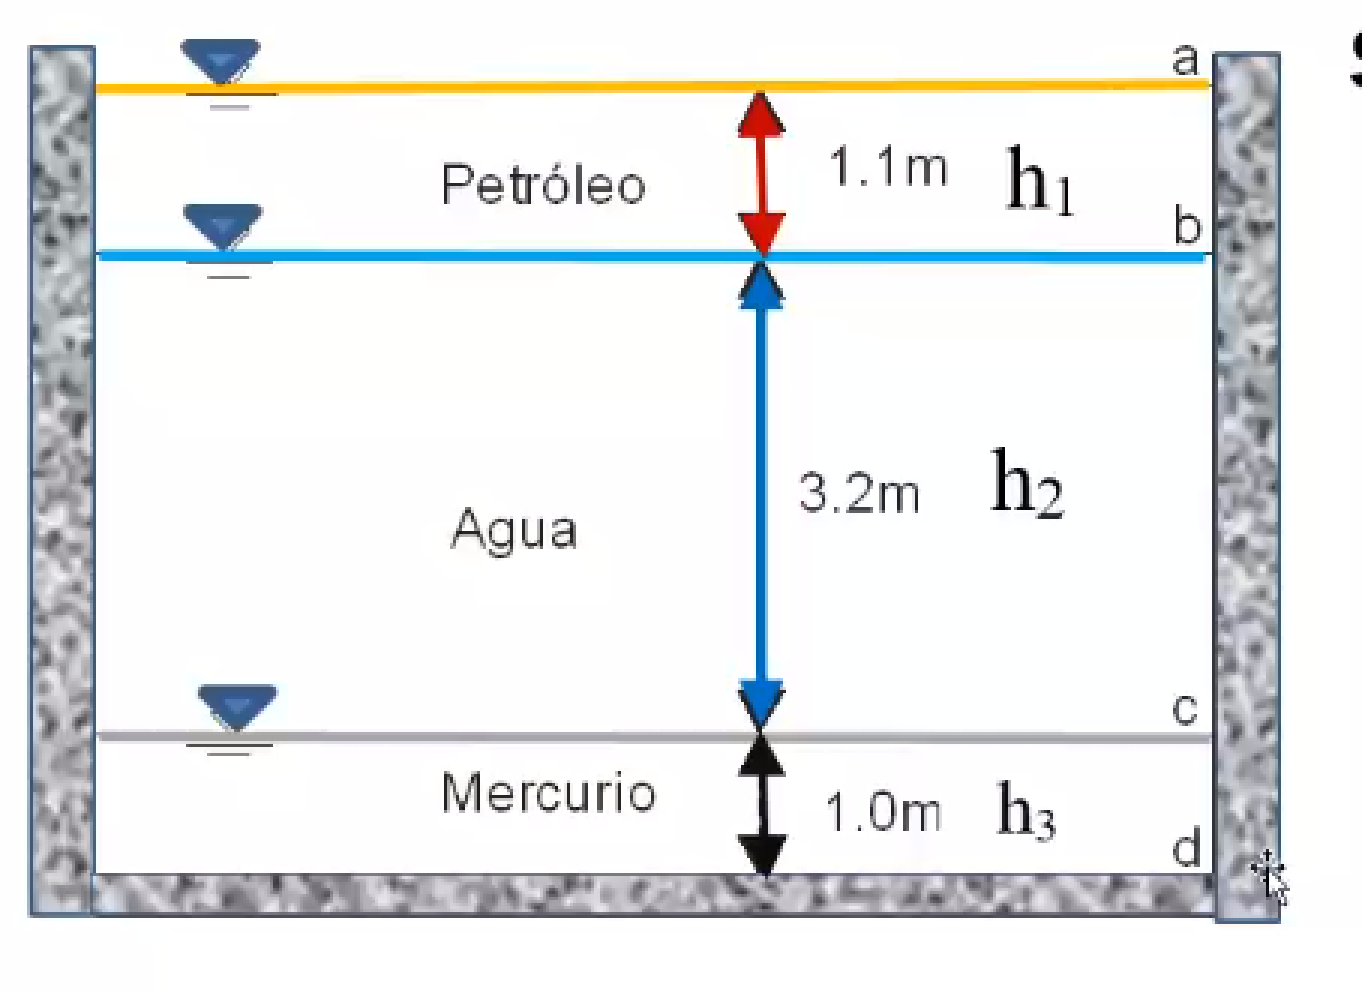
\includegraphics[width=0.5\textwidth]{hb12.png}}
  \caption{Diagrama del problema}
  \label{hb12}
\end{figure}

\textit{ Sol. }
\begin{align*}
    &P_d=P_c+\bar{\omega}_{Hg}\cdot h_3&&P_b=P_a+\bar{\omega}_{Ac}\cdot h\\
    &P_c=P_b+\bar{\omega}_{H2O}\cdot H_2&& P_a=0\\
    &P_d=\bar{\omega}_{Ac}\cdot h_1+\bar{\omega}_{H2O}\cdot h_2+\bar{\omega}_{Hg}\cdot h_3\\
    &P_d=900\frac{kg}{m^3}\cdot 1.1m+1,000\frac{kg}{m^3}\cdot 3.2m+13600\frac{kg}{m^3}\cdot 1m=17790\frac{kg}{m^2}
\end{align*}

Para el cálculo estructural y diseño de la pared del cajón, se requiere determinar el diagrama de cargas hidrostáticas que soporta. El cual se grafica a continuación:

\begin{figure}[h!]
  \centerline{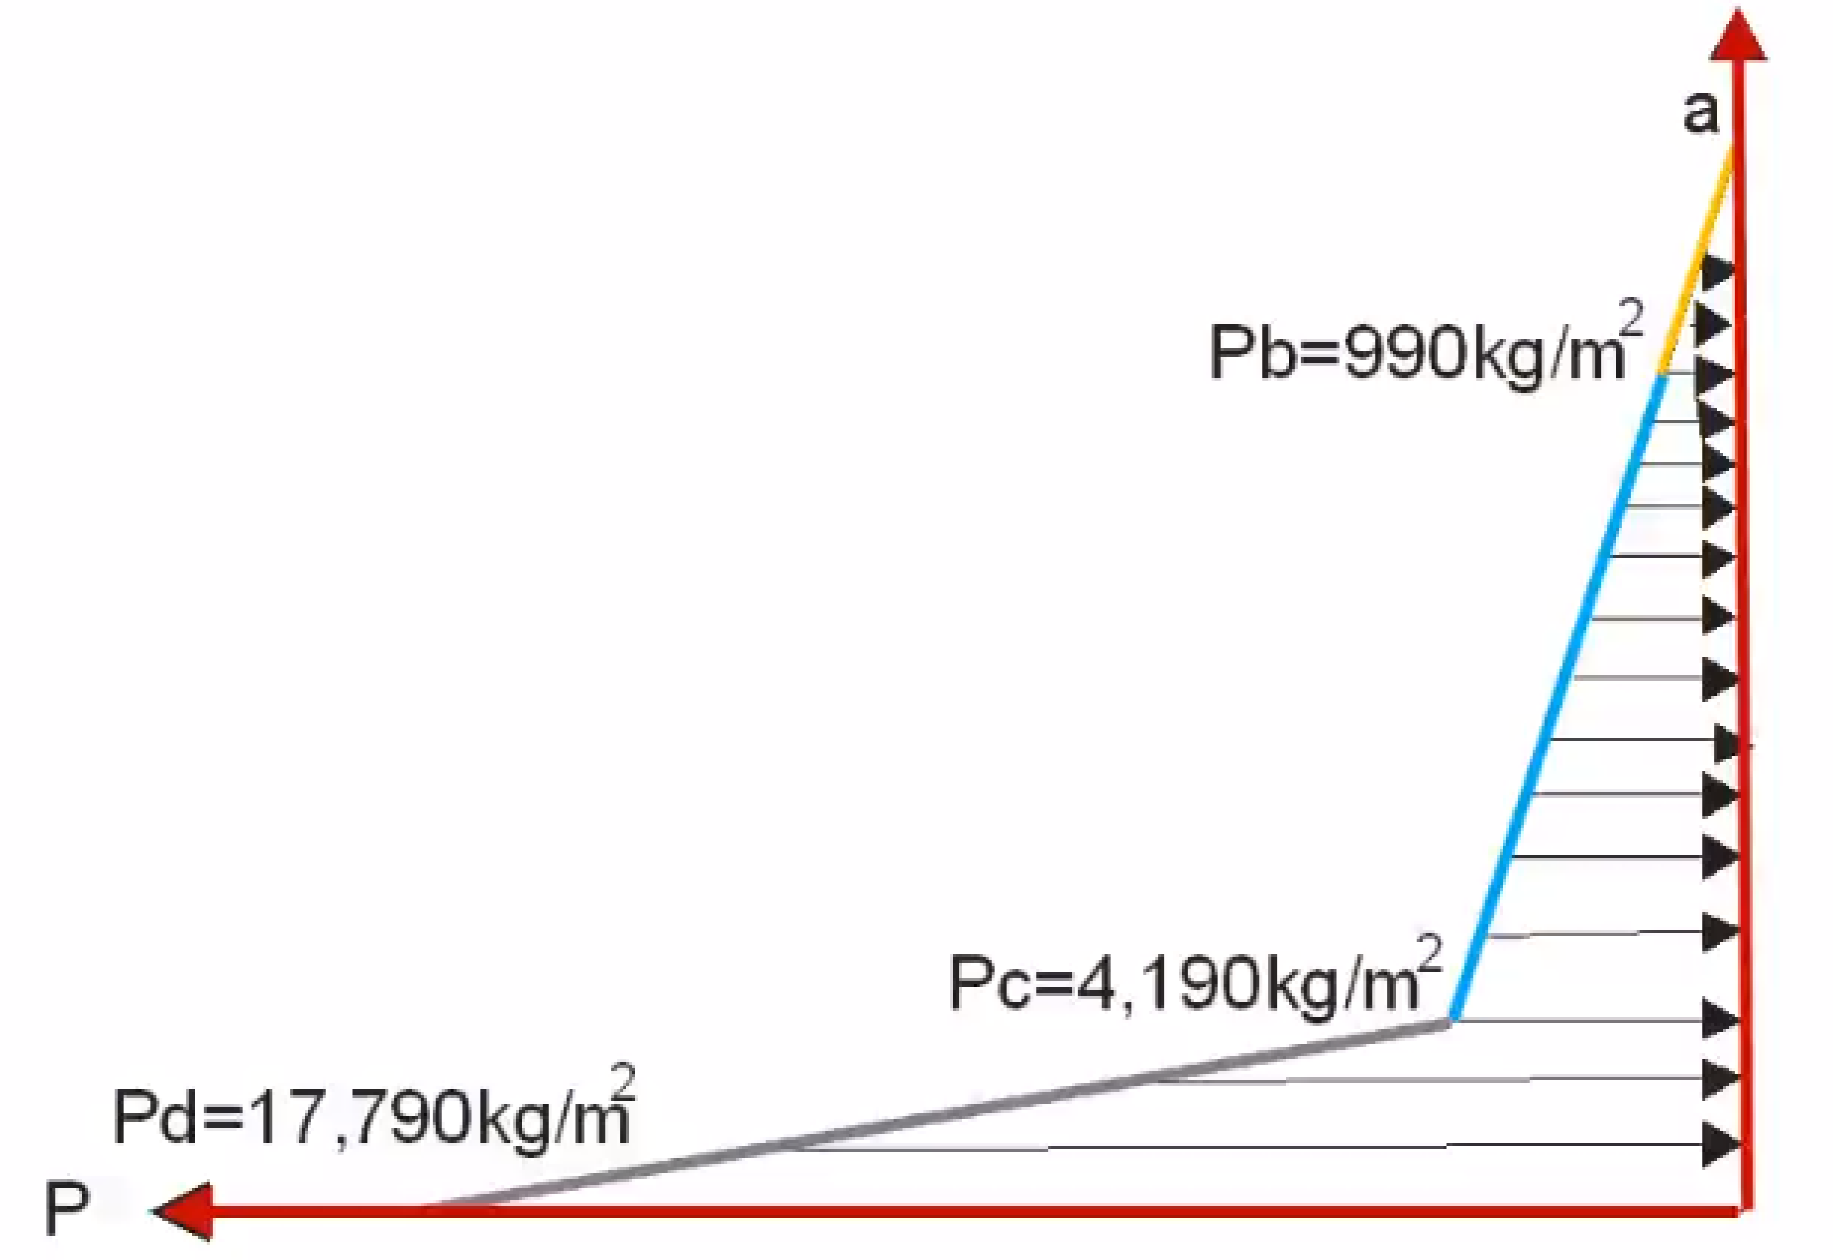
\includegraphics[width=0.5\textwidth]{hb13.png}}
  \caption{Gráfica de cargas hidrostáticas que soporta el cajón. En azul representa el agua}
  \label{hb13}
\end{figure}

\begin{figure}[h!]
  \centerline{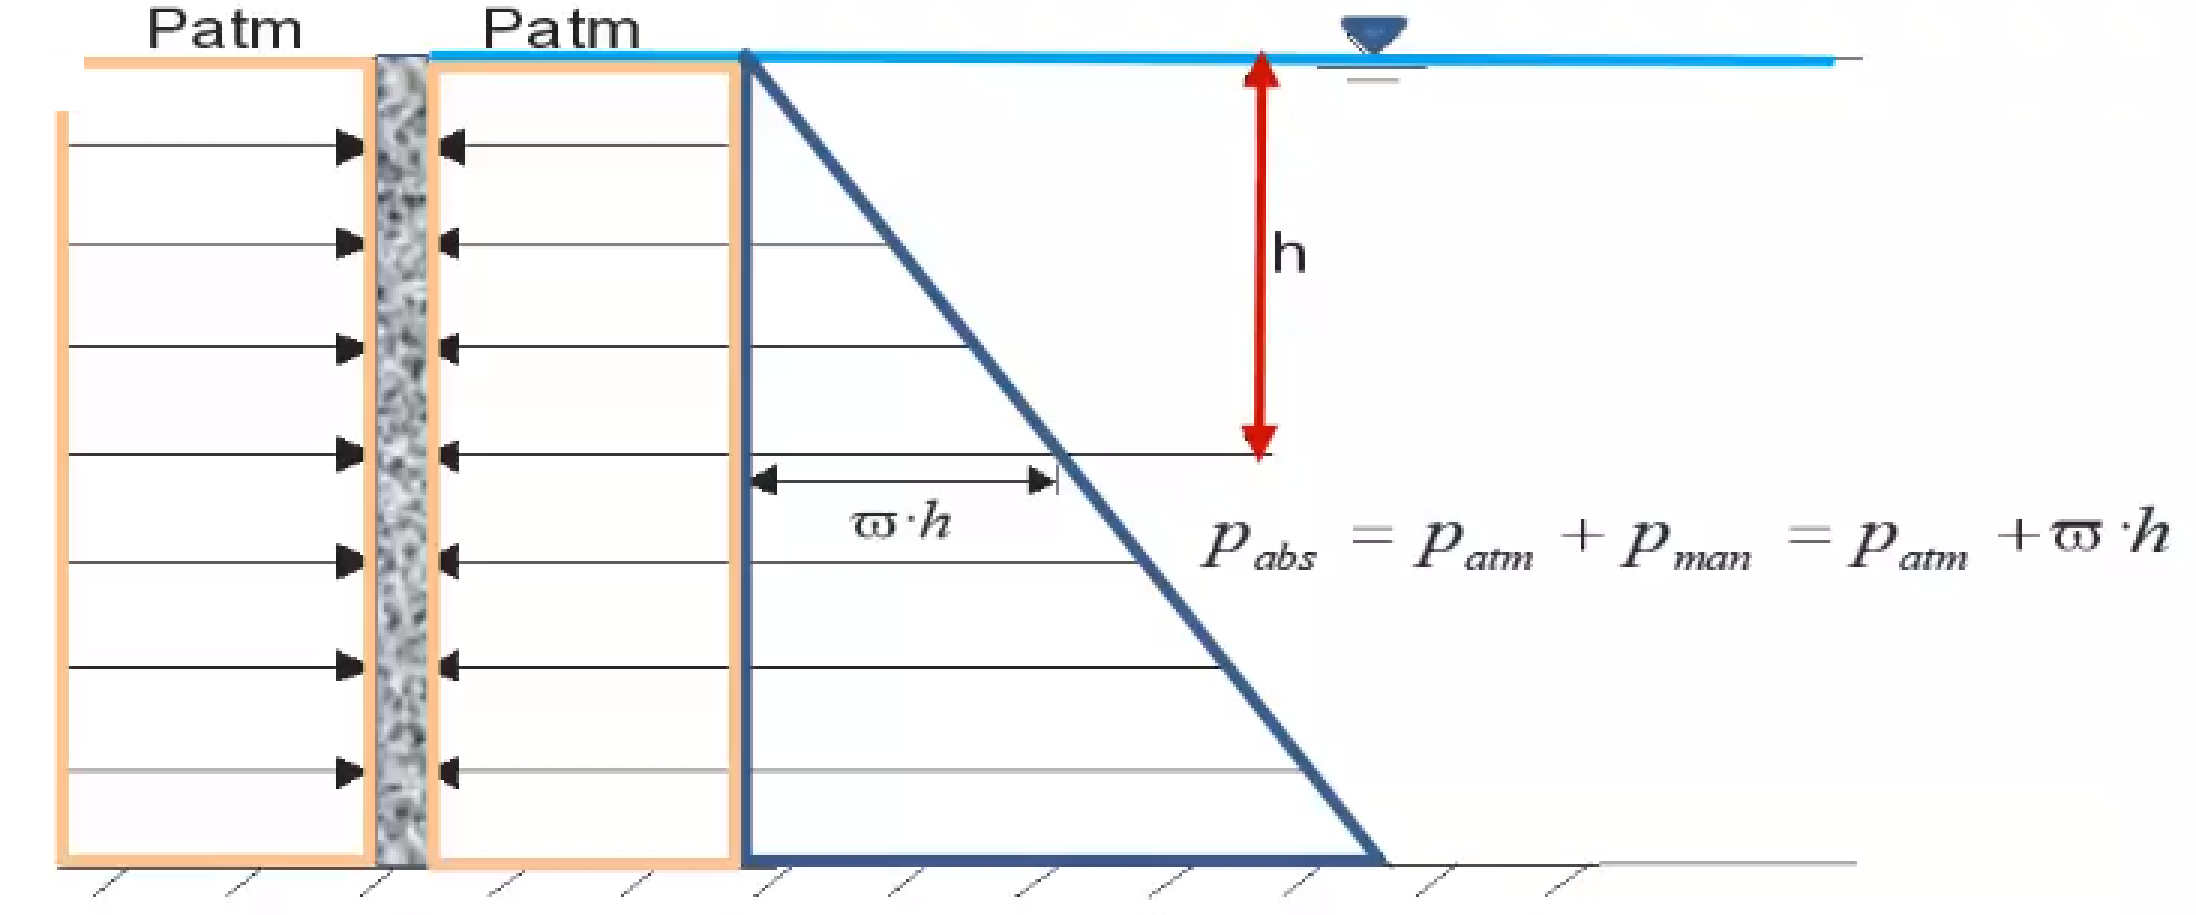
\includegraphics[width=0.5\textwidth]{hb14.png}}
  \caption{Diagrama de distribución de presiones}
  \label{hb14}
\end{figure}

\begin{equation}
    P_{abs}=P_{atm}+P_{man}+\bar{\omega}\cdot h
\end{equation}

\subsection{Dispositivos para medir presión}

Las presiones pueden expresarse con referencia a un origen arbitrario, lo orígenes más usuales son el vacío absoluto y la presión atmosférica, cuando se toma como origen el vacío absoluto, la presión se llama presión absoluta y cuando se toma como origen la presión atmosférica se le llama presión relativa o presión manométrica.

La presión atmosférica local depende de la altitud (elevación del sitio con respecto al nivel del mar), del lugar en que se encuentra el líquido, así como la densidad del aire.

\begin{equation}
    P_{atm}=10.33\left[1+\frac{z\left(6.95\times 10^{-8}z-1.288\times 10^{-3}\right)}{10.33}\right]
\end{equation}
Donde $z$ es la altitud y la presión en m.c.a.

La presión hidrostática que comúnmente se mide, es tomando como cero de referencia a la presión atmosférica local y a esta presión se le denomina manométrica

\subsubsection{Barómetro}

\begin{figure}[h!]
  \centerline{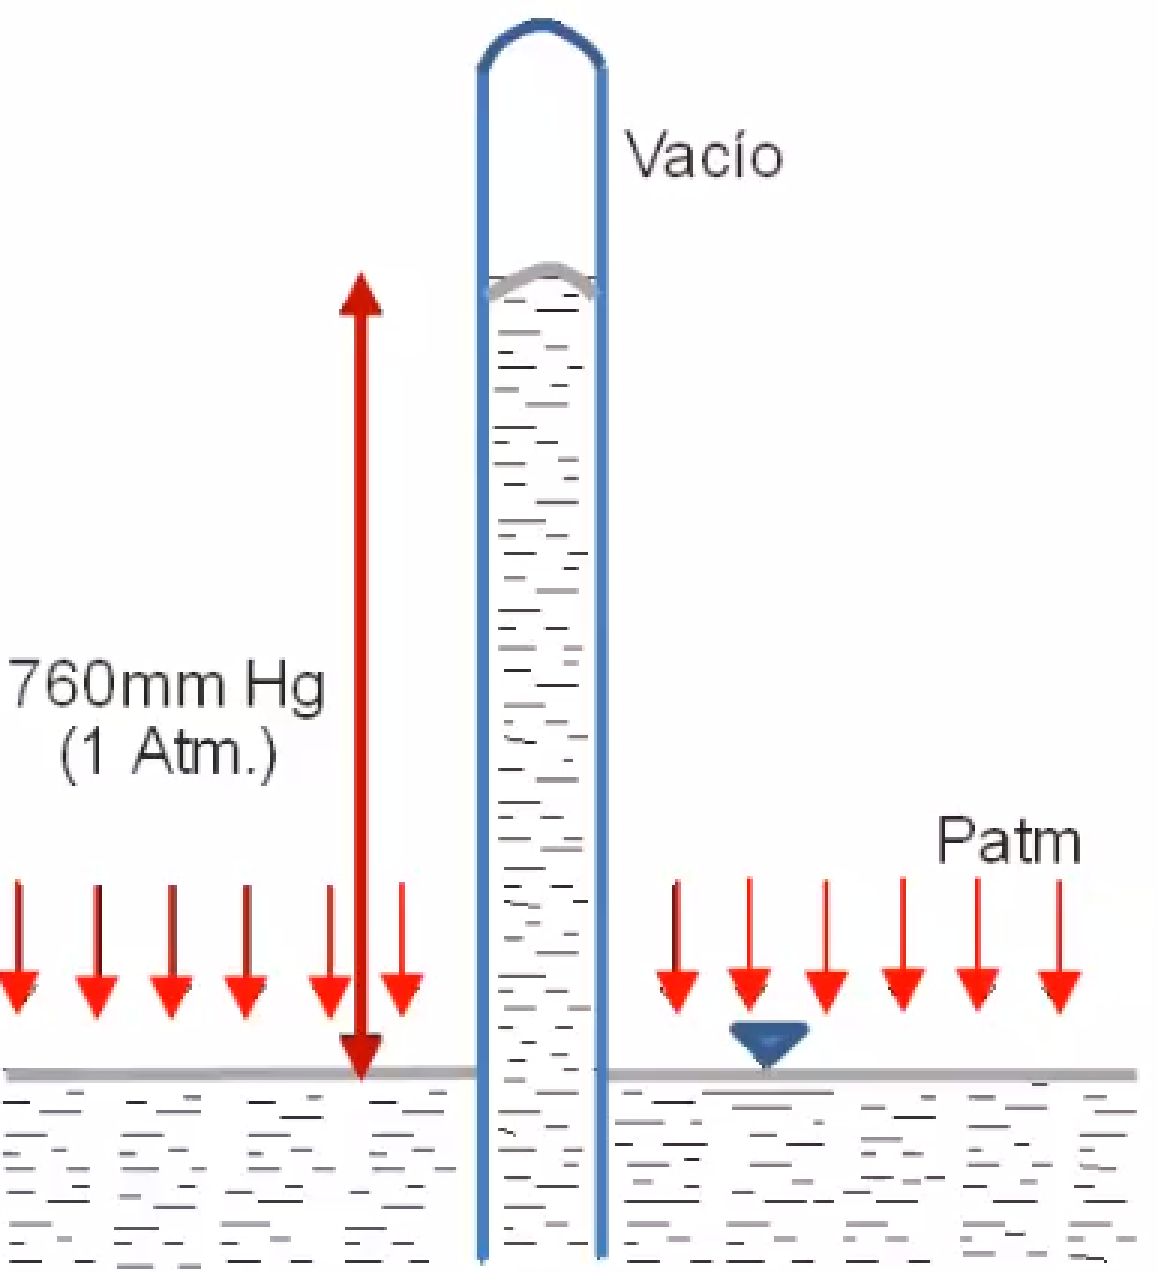
\includegraphics[width=0.5\textwidth]{hb15.png}}
  \caption{Barómetro}
  \label{hb15}
\end{figure}

\begin{example}
    \begin{equation*}
        p=\omega\cdot h=13595\cdot 0.76=10332.2kg/m^2=1atm=760mm\, Hg=10.33mca
    \end{equation*}
\end{example}

\subsubsection{Manómetros}

Los dispositivos para medir presiones relativas, se llaman manómetros y son tubos unidos a depósitos, tuberías o canales con el fin de medir su presión.

Los manómetros se clasifican en:

\begin{itemize}
    \item Simples
    \begin{itemize}
        \item Rama abierta
        \begin{itemize}
            \item Piezómetro 
            \item Tubo ``u''
        \end{itemize}
        \item Cerrados (manómetros de carátula)
    \end{itemize}
    \item Diferenciales
\end{itemize}

\textbf{Piezómetro:} Son manómetros simples de rama abierta cuya característica principal es que contienen solamente el líquido que pasa por el conducto, este consiste en un tubo transparente de cristal o plástico, recto o con un codo, de diámetro pequeño (mayor de 5mm para minimizar errores por ascenso capilar). Este tubo se conecta al punto en que se quiere medir la presión, practicando cuidadosamente en la pared del recipiente o tubería un orificio.
El líquido que lleva en su interior el conducto o depósito, asciende hasta alcanzar el equilibrio, determinándose entonces la presión mediante la distancia vertical $h$ desde el menisco (en la superficie del líquido), hasta el punto de interés.

\begin{figure}[h!]
  \centerline{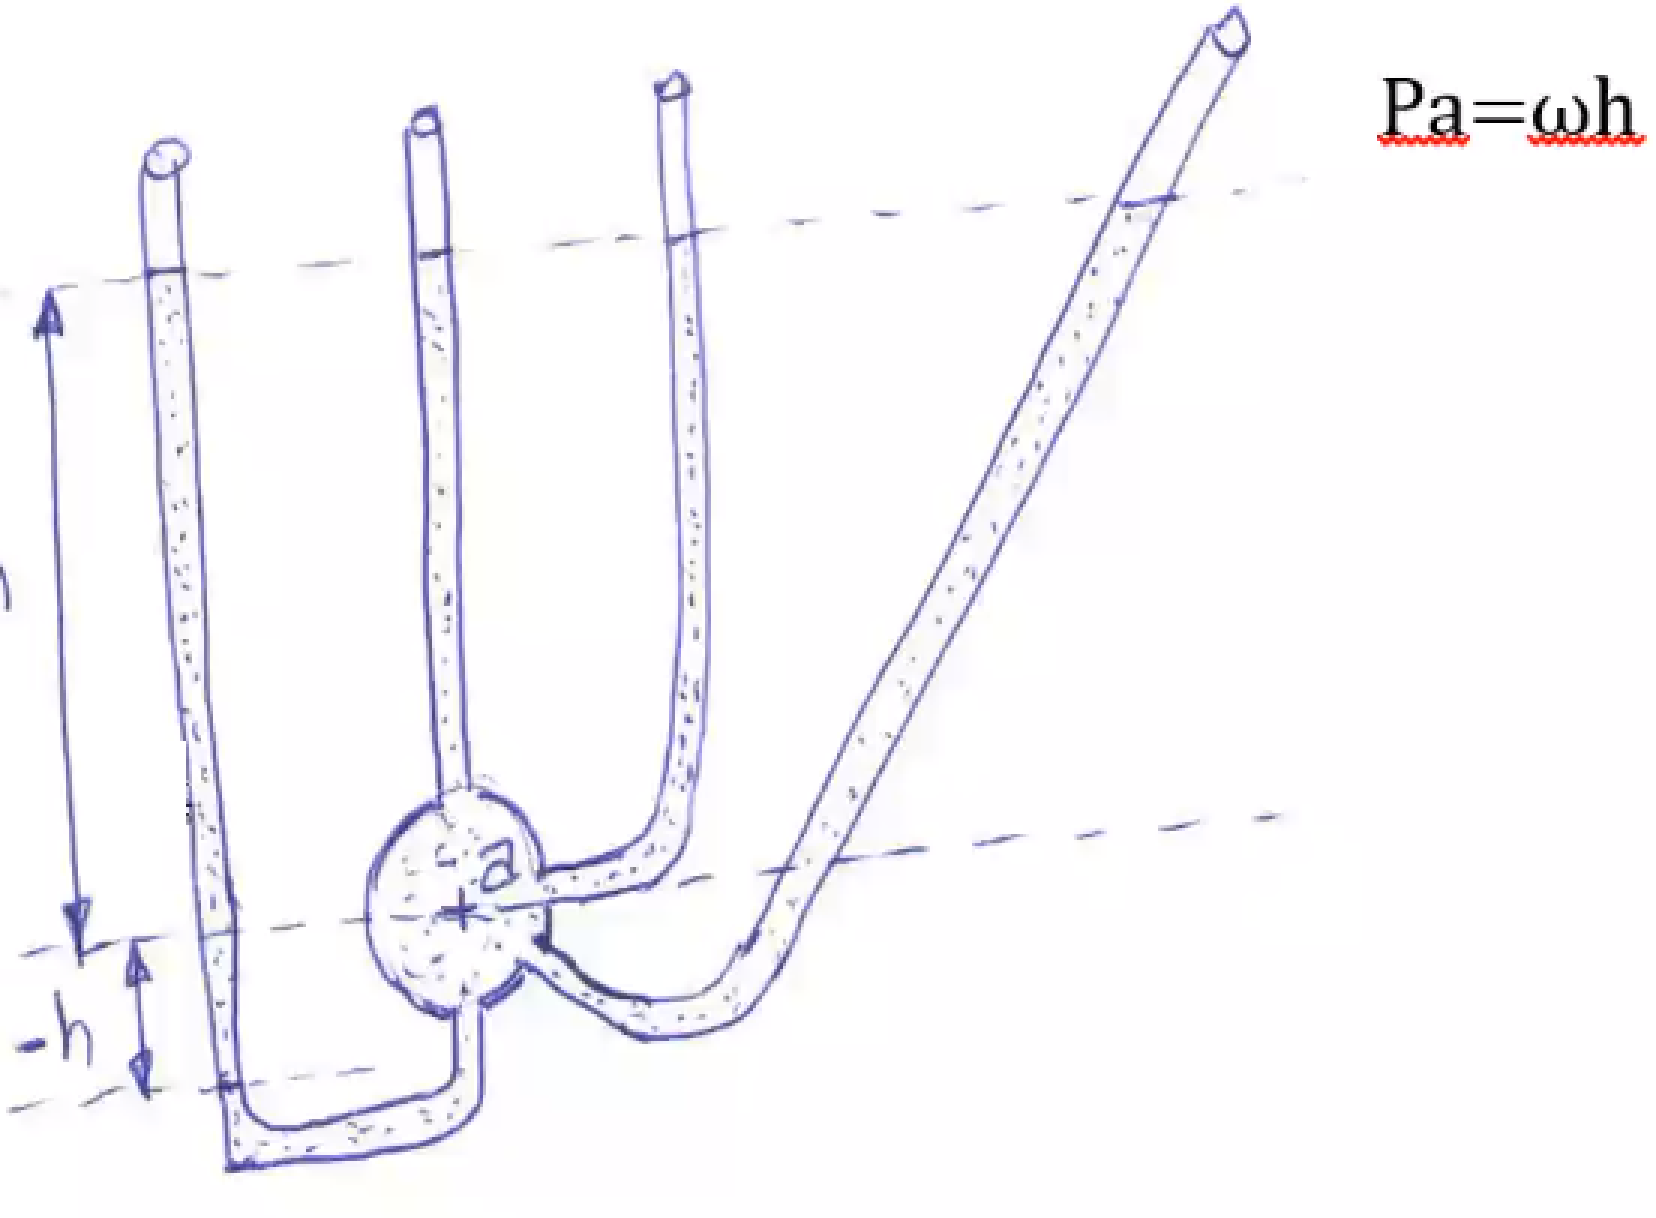
\includegraphics[width=0.5\textwidth]{hb16.png}}
  \caption{Piezómetro}
  \label{hb16}
\end{figure}

Estos dispositivos son medidores de presión muy precisos, pero no prácticos para la medición de grandes presiones, por la longitud excesiva de tubo que se requiere.

\textbf{Manómetros simples de tubo U:} con líquido más denso al fluido del conducto o depósito. Estos dispositivos se usan para medir grandes presiones, el líquido más usado es el mercurio, aunque algunas veces se pueden usar otros líquidos para medir pequeñas presiones. Agua alcohol (coloreados)
tetrabromuro de acetileno o bencina, más densos que el fluido circulante en el conducto, siempre que los dos no sean mezclables entre sí.


\begin{align}
    &p_a=\Delta h\cdot \bar{\omega}^{\prime}-z\cdot \bar{\omega}\\
    &p_b=-\Delta h\cdot \bar{\omega}^{\prime}-z\cdot \bar{\omega}
\end{align}

\textbf{Manómetro simple cerrado:} Un manómetro de este tipo es el manómetro tipo Bourdon (metálico de carátula) es un aparato integrado por una carátula y una aguja que es accionada por elemento que soporta la presión, este es un tubo metálico curvado, cerrado por un extremo y por el otro se conecta al recipiente que contiene el fluido cuya presión va a medirse. La carátula puede ser graduada con las unidades que se prefieran tales como $\frac{kg}{cm^2}$, $mm$ de mercurio, metros de agua $lb/pulg^2(PSI)$ u otros. 
pueden medir presiones más altas y práctico de portar, algunas desventajas con respecto a los anteriores, son que pueden ser más costosos y sufrir una descalibración, por lo que tienen que ajustarse periódicamente.\footnote{Una presión aceptable es cuando el error no es mayor al 5\%}

\textbf{Manómetro diferencial:}
%%%%
Método americano:
\begin{align}
    &p_a+\bar{\omega}_1\cdot h_1-\bar{\omega}_3\cdot h_3-\bar{\omega}_2\cdot h_2=p_b\\
    &p_b-p_a=\bar{\omega}_1\cdot h_1-\bar{\omega}_3\cdot h_3-\bar{\omega}_2\cdot h_2
\end{align}

Método del plano de equilibrio
\begin{align*}
    &p_1=p_2\\
    &p_1=p_a+\bar{\omega}_1\cdot h_1\\
    &p_2=p_b+\bar{\omega}_3\cdot h_3+\bar{\omega}_2\cdot h\\
    &p_b-p_a=\bar{\omega}_1\cdot h_1-\bar{\omega}_3\cdot h_3-\bar{\omega}_2\cdot h_2
\end{align*}


\begin{example}
    Determine:
\begin{enumerate}
    \item Diferencia de presiones entre a y b
    \item Si $p_h=2.3\times 10^4$ Pa el valor de la presión en a en m.c.a
    \item $p_a$ en PSI
    \item $p_a$ en bar
    \item $p_a$ en atm
    \item $p_a$ en $\frac{kg}{cm^2}$
    \item $p_a$ en Torr
\end{enumerate}

\end{example}

\textit{ Sol. }

\begin{enumerate}
    \item Aplicando el método americano
    \begin{align*}
        &p_a+\omega h_1-\omega_{Hg}h_2-\omega_{aire}h_3+\omega_{Ac}h_4=p_b\\
        &p_a-p_b=-\omega h_1+\omega_{Hg}h_2+\omega_{aire}h_3-\omega_{Ac}h_4\\
        &p_a-p_b=-1,000\frac{kg}{m^3}\left(2\cdot 0.3048m\right)+13600\frac{kg}{m^3}\left(27\cdot 0.0254m\right)-860 \frac{kg}{m^3}(0.27)\\
        &p_a-p_b=8185.1 \frac{kg}{m^2}=83238.6 \frac{N}{m^2}
    \end{align*}
    \item Si $P_b=2.310^4$Pa, el valor de la presión en a en m.c.a:
    \begin{align*}
        &p_a-p_b=83238.6\frac{N}{m^2}\\
        &p_a=83238.6\frac{N}{m^2}+23,000Pa=106.239kPa\\
        &p_a=106239\frac{N}{m^2}\left(\frac{1kg}{9.81}\right)=10829.6\frac{kg}{m^2}\\
        &h=\frac{p}{\omega}\implies \frac{10829.6\frac{kg}{m^2}}{1,000\frac{kg}{m^3}}=10.83mca
    \end{align*}
    \item $p_a$ en PSI
    \begin{equation*}
        p_a=10829.6\frac{kg}{m^2}\left(\frac{1lb}{0.4536kg}\right)\left(\frac{0.0254m}{1pulg}\right)^2=15.403PSI
    \end{equation*}
    \item $p_a$ en bar
    \begin{equation*}
        p_a=106239pa\left(\frac{1bar}{100,000Pa}\right)=1.062bar
    \end{equation*}
    \item $p_a$ en atm
    \begin{equation*}
        p_a=10.83mca\left(\frac{1atm}{10.33mca}\right)=1.048Atm
    \end{equation*}
    \item $p_a$ en $\frac{kg}{cm^2}$
    \begin{equation*}
        p_a=10829.6\frac{kg}{m^2}\left(\frac{1m}{100cm}\right)^2=1.083\frac{kg}{cm^2}
    \end{equation*}
    \item $p_a$ en Torr
    \begin{equation*}
        h=\frac{10829.6\frac{kg}{m^2}}{13600\frac{kg}{m^3}}=0.7963m=796.3Terr
    \end{equation*}
\end{enumerate}

\begin{problem}
    ¿Dónde se localiza la presión hidrostática con valor de cero y cuanto vale la presión en centro del tubo?
\end{problem}
\begin{align*}
    &x=0\quad p=0\\
    &p_x=h_3\omega -x\omega_{Hg}=0\\
    &x=\frac{h_3\omega}{\omega_{Hg}}\leq h_2\\
    &p_{x\prime}h_3\omega-h_2\omega_{Hg}-x^{\prime}\omega^{\prime}=t\\
    &x^{\prime}=\frac{h_3\omega-h_2\omega_{Hg}}{\omega^{\prime}}\leq h_1
\end{align*}

\subsection{Centroides y momentos de áreas}
El centroide de una superficie plana, y los diferentes momentos se definen con las siguientes ecuaciones:
\begin{align}
    X_cA=\int x\, dA&& Y_cA =\int y\, dA
\end{align}
\begin{align*}
    x_c=\frac{\int x\, dA}{A}=\frac{M_y}{A}&&y_c=\frac{\int y\, dA}{A}=\frac{M_x}{A}
\end{align*}
Los momentos estáticos o primer momento:
\begin{align*}
    &M_x=\int y\, dA\\
    &M_y=\int x\, dA
\end{align*}
\begin{align*}
    &\text{Momento de inercia}&&\text{Producto de inercia}\\
    &I_X=\int y^2\, dA&&I_{XY}=\int xy\, dA\\
    &I_Y=\int x^2\, dA&&
\end{align*}

\begin{theorem}[Teorema de Steiner para momentos y productos de inercia]
    Para el momento de inercia con respecto al eje $y$ se tiene: 
    \begin{align*}
        &I_Y=\int x^2\, dA=\int \left(\bar{x}+X_c\right)^2\, dA\\
        &I_y=\int \left(\bar{x}^2+2\bar{x}X_c+X^1_c\right)\, dA=\bar{X}^2\int \, dA+2\bar{X}\int X_c\, dA+\int X^2_c\, dA
    \end{align*}
    \begin{equation}
        I_y=\bar{X}^2A+\bar{I}_Y
    \end{equation}
    De igual forma para el momento de inercia con respecto al eje X
    \begin{equation}
        I_x=\bar{Y}^2A+\bar{I}_x
    \end{equation}
    Para el producto de inercia con respecto a los ejes $XY$ se tiene:
    \begin{align*}
        &I_{XY}=\int XY\, dA=\int \left(\bar{X}+X_c\right)\left(\bar{Y}+Y_c\right)\, dA\\
        &I_{XY}=\int XY\, dA=\int \bar{X}\bar{Y}+\bar{X}Y_c+X_cY_c\,dA=\bar{X}\bar{Y}\int dA+\bar{X}\int Y_c\, dA+\bar{Y}\int X_c\, dA+\int X_cY_c\,dA
    \end{align*}
    \begin{equation}
        I_{XY}=\bar{X}\bar{Y}A+\bar{I}_{XY}
    \end{equation}
\end{theorem}

\subsubsection{Empuje hidrostático sobre superficies planas}

En el diseño de dispositivos y objetos sumergidos es necesario calcular las magnitudes y ubicaciones de las fuerzas que actúan tanto
líquido sobre la superficie plana se encuentra integrando 

\begin{figure}[h!]
    \centering
    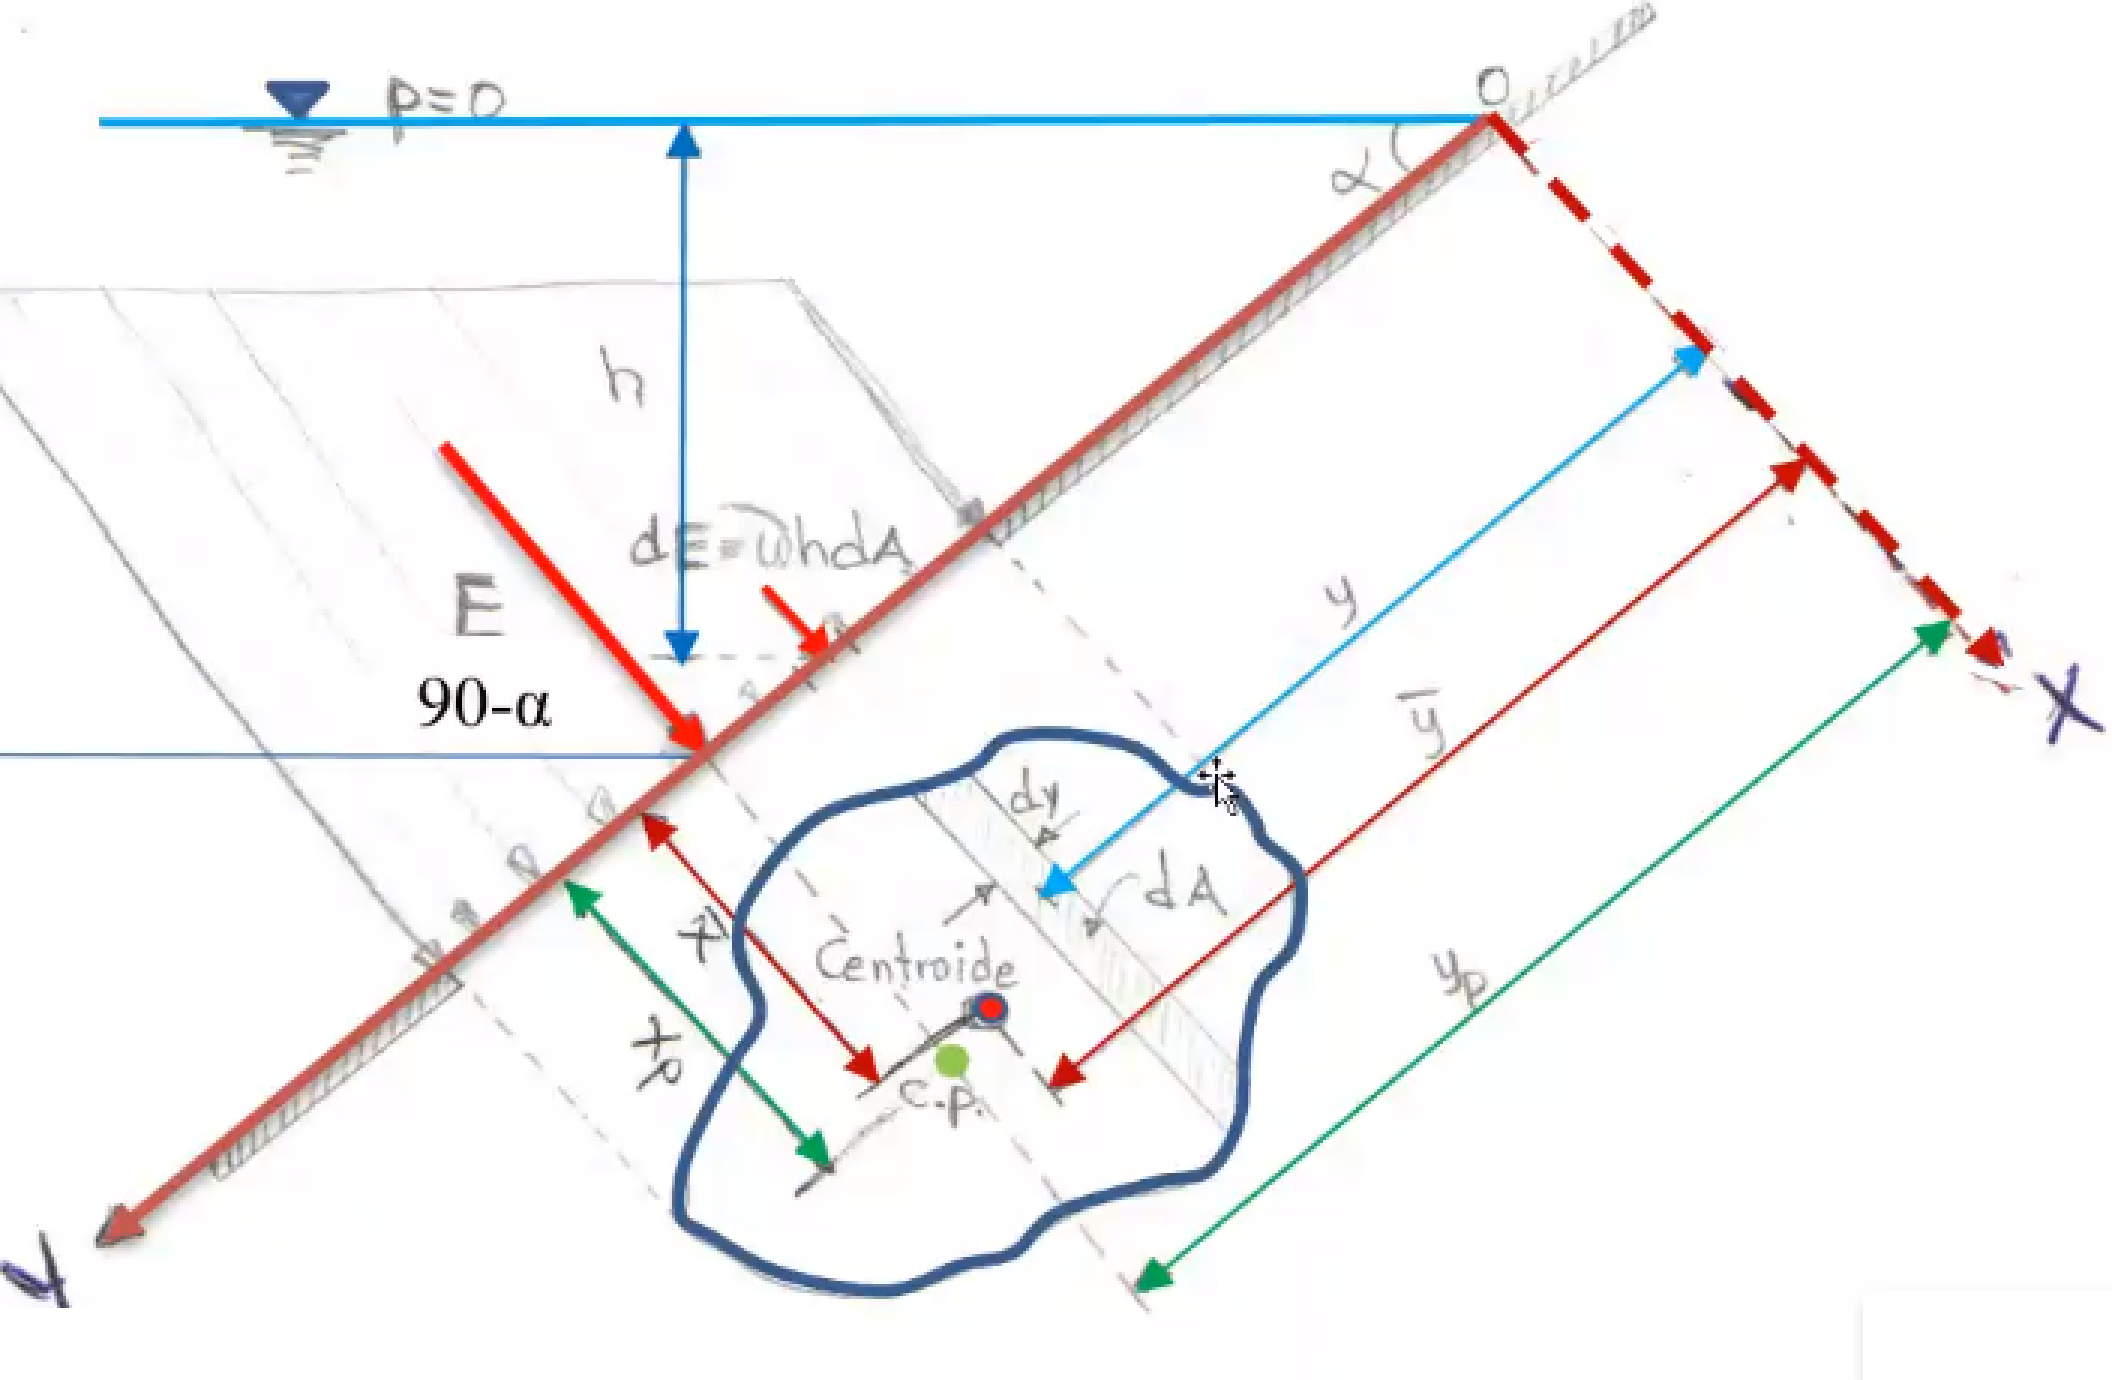
\includegraphics[width=0.5 \textwidth]{hb17.png}
    \caption{Empuje hidrostático sobre superficies planas}
    \label{hb17}
\end{figure}

Las características vectoriales del empuje son: 

\begin{itemize}
    \item Magnitud
    \item Dirección
    \item Sentido
    \item Punto de aplicación
\end{itemize}

\begin{align*}
    &dE=pdA&&E=\int p\, dA
\end{align*}

donde en general, se utiliza la presión manométrica. La presión atmosférica se elimina puesto que actúa en ambos lados de la superficie con la misma intensidad y direcciones opuestas. Las coordenadas $xy$ están en el plano de la superficie plana. Suponiendo $(h,p)=(0,0)$, se sabe que
\begin{equation}
    p=\bar{omega}\cdot h=\bar{\omega}\cdot y\sin{(\alpha)}
\end{equation}

donde $h$ mide verticalmente hacia abajo desde la superficie libre, hasta el elemento $dA$ y $y$ se mide desde el punto 0 en la superficie libre. Entonces la fuerza se expresa como: 
\begin{equation*}
    E=\int\omega h\, dA=\int \omega y\sin{(\alpha)} dA=\omega \sin{( \alpha )}\int y\, dA=\omega\sin{( \alpha )} M_x
\end{equation*}
La distancia al centroide se define como: 

\begin{equation*}
    \bar{y}=\frac{\int_A y\, dA}{A}\implies A\bar{y}=\int_A y\, dA
\end{equation*}
Por lo tanto $E=\omega\sin{(\alpha)}M_x=\omega \sin{( \alpha )}\bar{y}A$

donde $h$ es la distancia vertical de la superficie libre al centroide del área y $p_c$ es la presión en el centroide. De este modo se ve que la magnitud del empuje sobre la superficie plana es la presión en el centroide multiplicada por el área. La fuerza no actúa en el centroide.
Para hallar la ubicación de la fuerza resultante $F$, se observa que la suma de los momentos de todas las fuerzas de presión infinitesimales que actúan en el área A deben ser iguales al momento de la fuerza resultante. Sea $F$ la fuerza que actúa en el punto $(x_p,y_p)$ en el centro de presión $c.p$. El valor de la $y_p$ se obtiene igualando los momentos con respecto al eje $x$

\begin{equation*}
    Y_{CP}E=\int yp\, dA=\int y^2\,dA=\omega\sin{(\alpha)}I_x
\end{equation*}
El segundo momento de un área con respecto a un eje está relacionado con el segundo momento de la misma área con respecto a un eje paralelo que pasa por su centroide por medio del denominado Teorema de los ejes paralelos, mediante la expresión: 

\begin{equation}
    I_x=\bar{I}_x+A\cdot \bar{y}^{2}
\end{equation}

\begin{equation*}
    y_{cp}=\frac{\omega\sin{( \alpha )}I_x}{\omega\sin{( \alpha )}M_x}=\frac{I_x}{M_x}=\frac{\bar{y}^2A+\bar{I}_x}{\bar{y}A}=\bar{y}+\frac{\bar{I}_x}{\bar{y}A}
\end{equation*}

Observe en la ecuación anterior que $y_p$ será siempre mayor a $\bar{y}$ ASí mismo, para localizar la coordenada $x_p$ del centro de presiones: 

\begin{equation*}
    x_{cp}=\frac{\omega\sin{( \alpha )}I_x}{\omega\sin{( \alpha )}M_x}=\frac{I_{xy}}{M_x}=\frac{\bar{y}\bar{x}A+\bar{I}_{xy}}{\bar{y}A}=\bar{x}+\frac{\bar{I}_{xy}}{\bar{y}A}
\end{equation*}
Generalmente, las superficies sobre las que se desea calcular el empuje hidrostático son simétricas respecto de un eje paralelo al eje $y$. Esto hace que $\bar{I}_{xy}=0$, y que el centro de presiones quede sobre dicho eje. 

\begin{problem}[Obtener los empujes]
    hidrostáticos por unidad de ancho, así como los centros de presiones sobre las caras, $a_1$ es vertical y $a_2$ inclinado, el empuje total horizontal sobre el muro mostrado en la figura y el factor de seguridad al volteo. El bordo libre es de 0.5m y la gravedad específica de la cortina (simétrica) es de 2.4
\end{problem}

\begin{figure}[h!]
\centering
  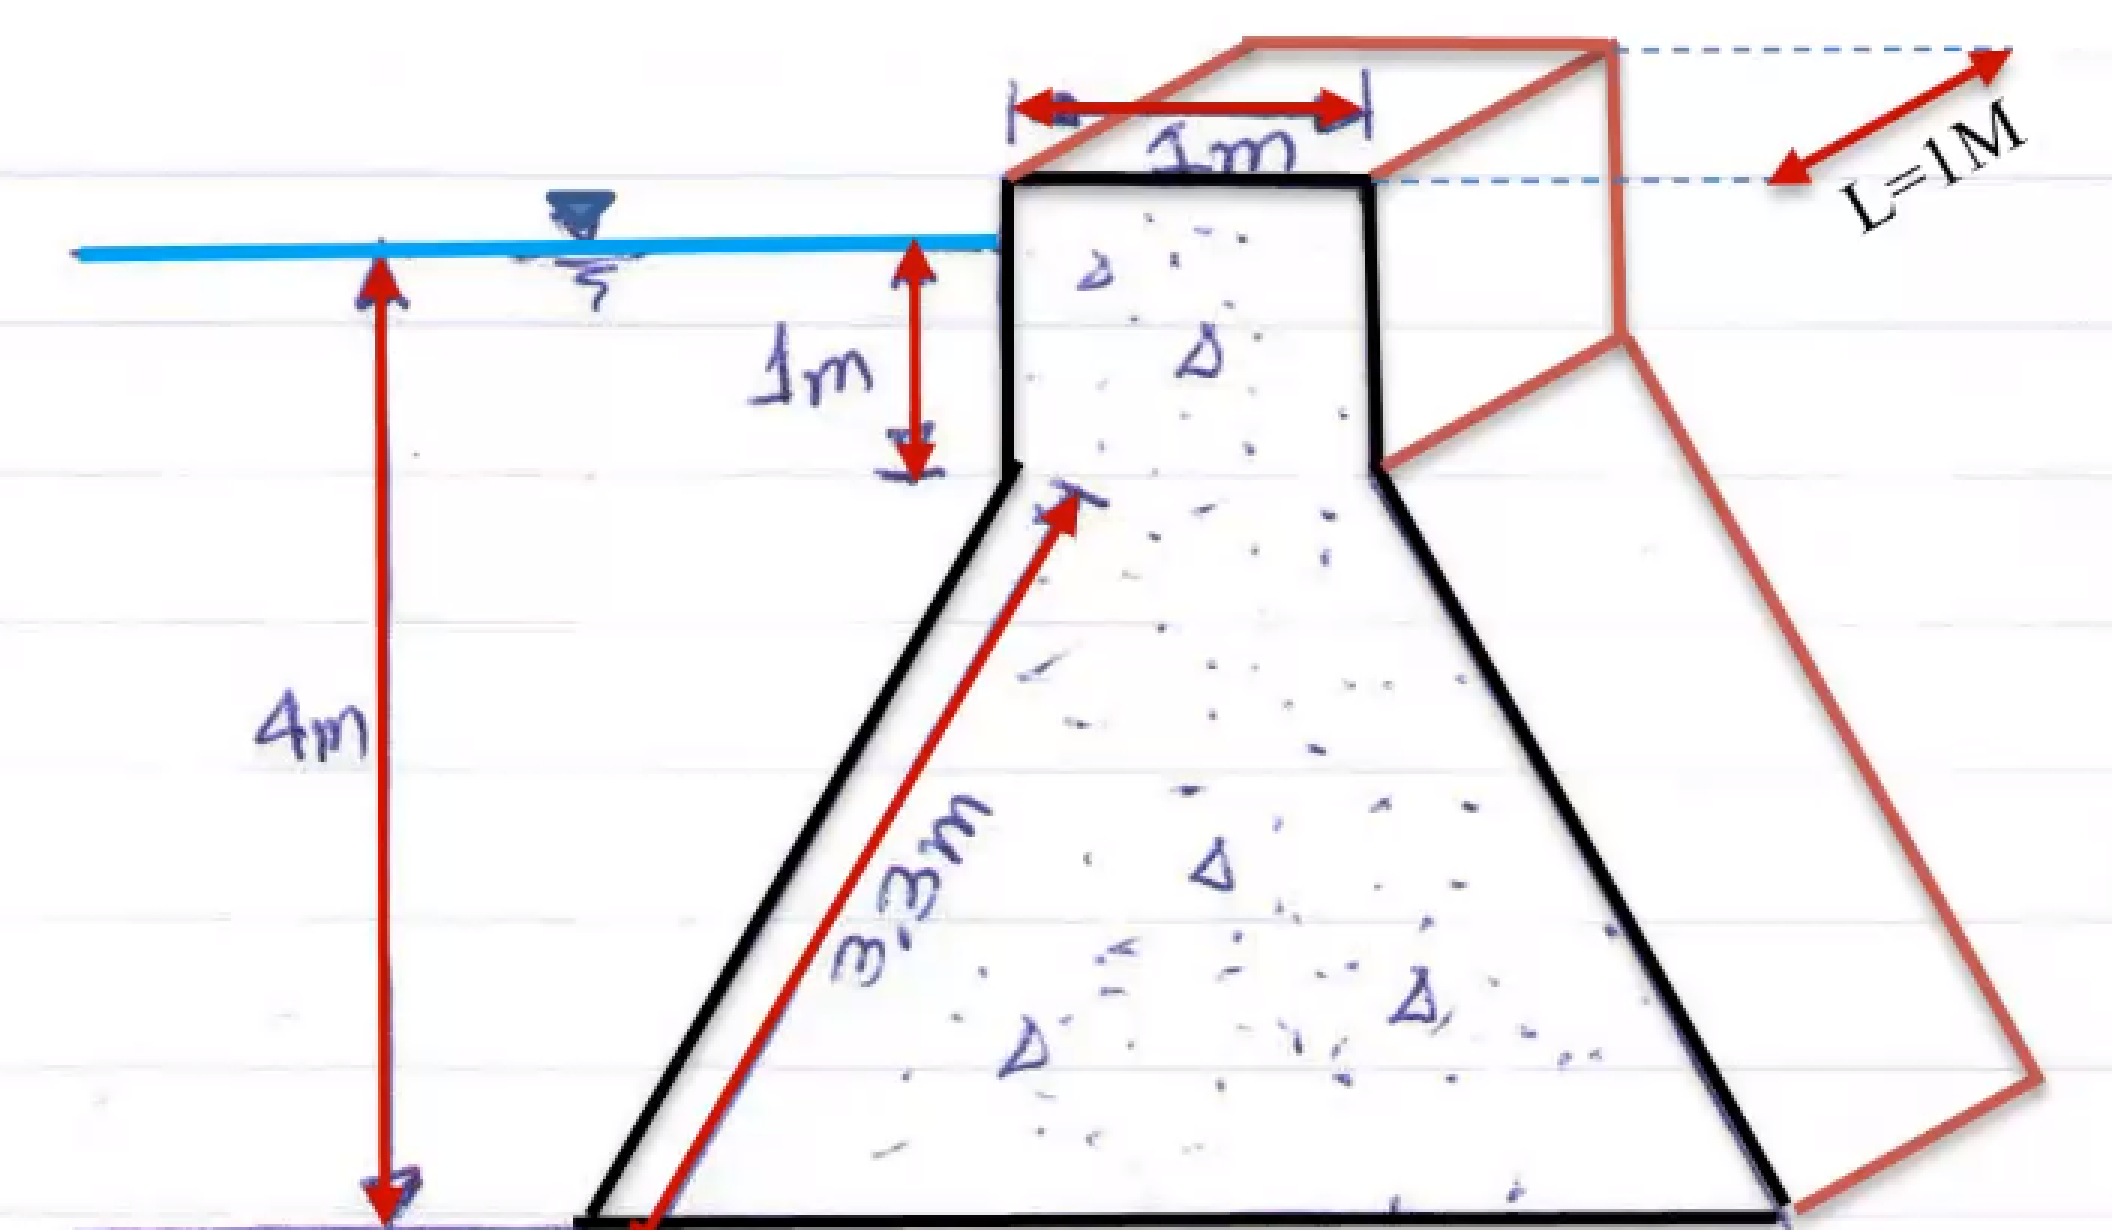
\includegraphics[width=0.5\textwidth]{hb18.png}
  \caption{Esquema del problema}
  \label{hb18}
\end{figure}

\textit{ Sol. }

\begin{figure}[h!]
\centering
  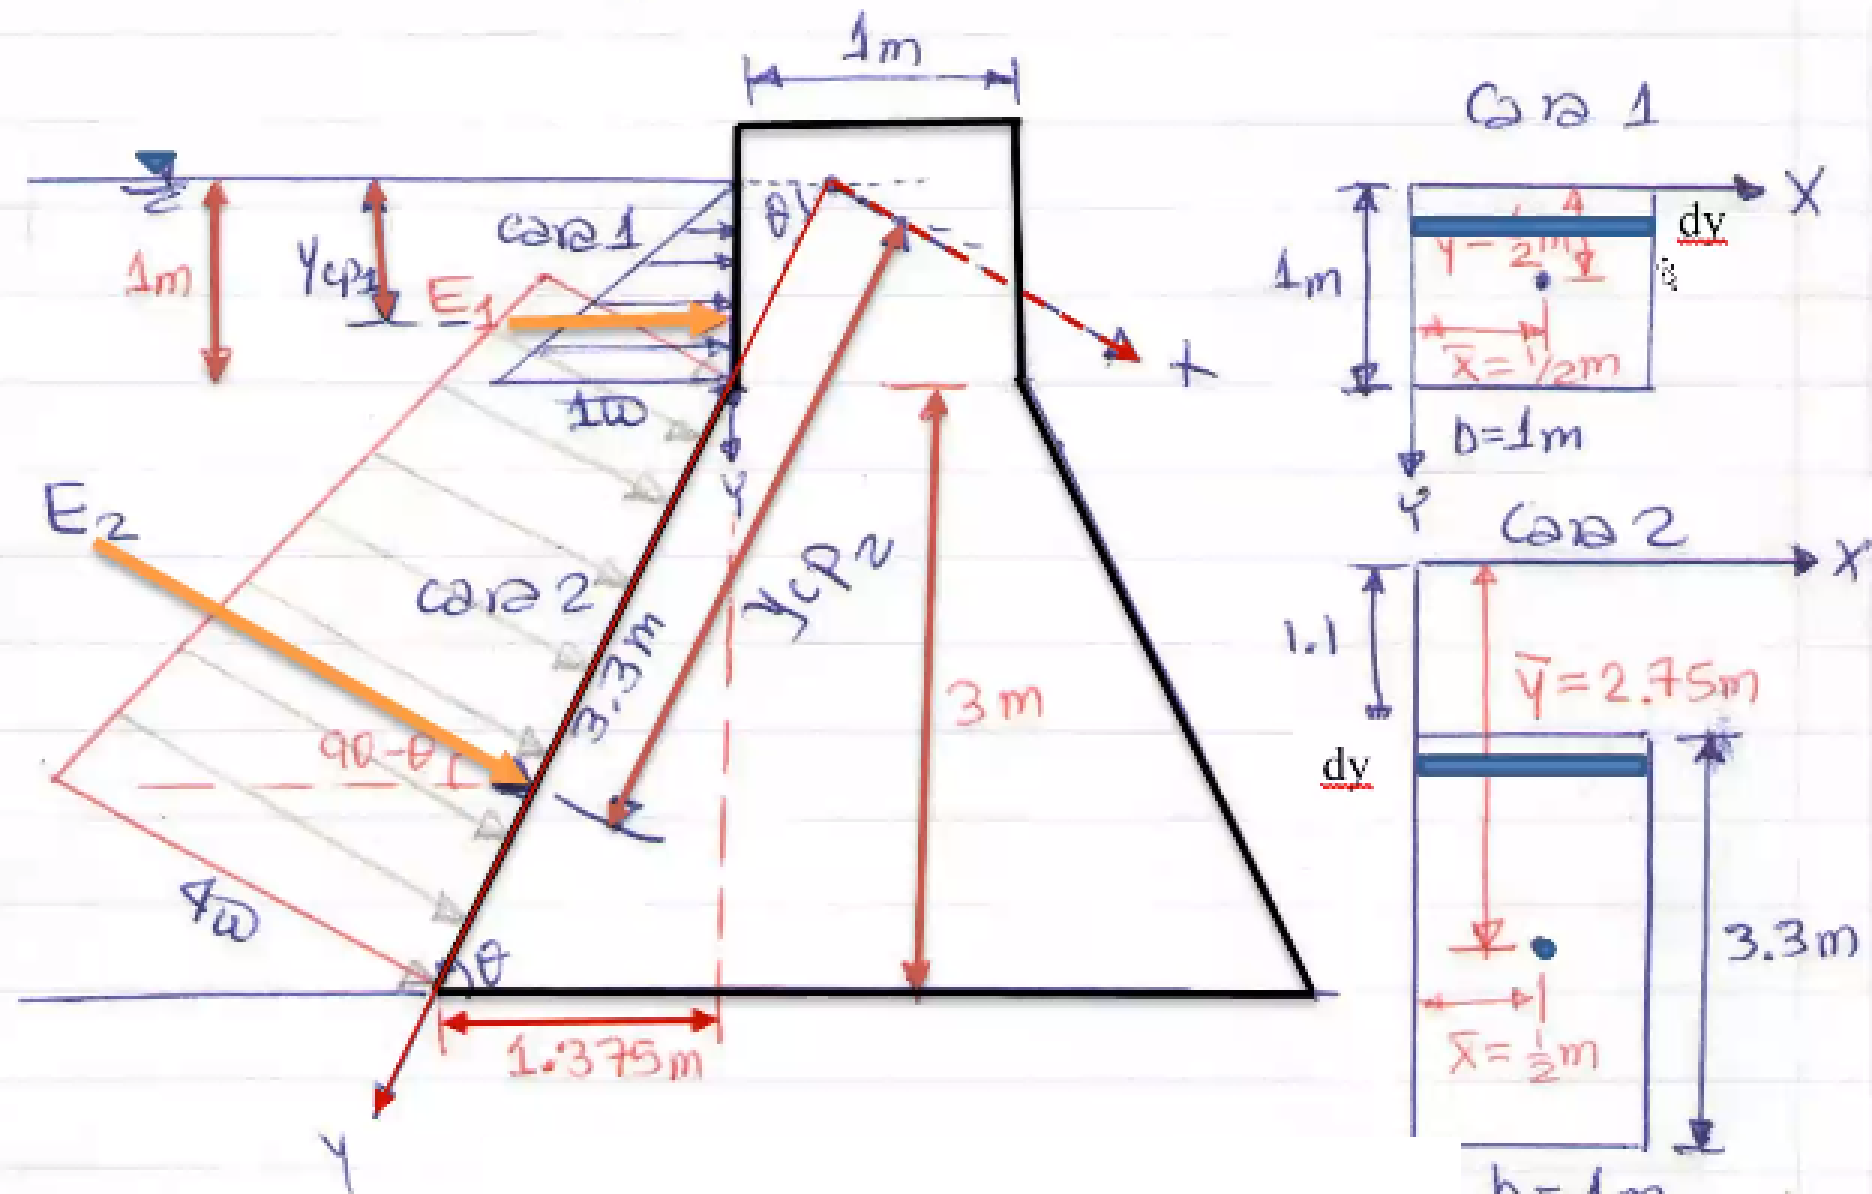
\includegraphics[width=0.5\textwidth]{hb19.png}
  \caption{Esquema de la solución del problema}
  \label{hb19}
\end{figure}

Para la cara $a_1$, $h=y$, la magnitud del vector de empuje es: 

\begin{equation*}
    E_1=\int p\, dA=\int_0^1\omega yb\,dy=\omega b\int_0^1y\, dy=\omega b\left\lvert \frac{y^2}{2}\right\rvert_0^1=\frac{1ton}{m^3}\cdot 1,\cdot\frac{(1m)^2}{2}=0.5ton
\end{equation*}

El empuje se describe como: 

\begin{equation*}
    E_1=\omega\ddot{y}\sin{(\theta)}A=1,000\frac{kg}{m^3}\cdot 0.5m\cdot \sin{(90^{\circ})}\cdot 1m^2=500kg
\end{equation*}

El empuje también se obtiene con el volumen del diagrama de presiones, el cual es un prisma triangular. De altura $h$,base es $\omega h$ y ancho $L=1$. $E_1\frac{h\cdot\omega h}{2}\, L=\frac{1m\cdot 2 ton/m^3\cdot 1m}{1m}=0.5ton$

Su localización $x_{cp1},y_{cp1}$ es:
\begin{align*}
    &y_{cp1}E_1=\int yp\,dA=\int y\omega y\, dA=\omega\int y^1\, dA=\omega I_x=\frac{\omega I_x}{E_1}=y_{ycp1}\\
    &I_x=\int_A y^1\, DA=b\int_0^1 y^2\, dt=\frac{b}{3}y^3\mid_0^1=\frac{1m\cdot 1m^3}{3}=\frac{1}{3}m^4\\
    &y_{cp1}=\frac{\frac{1,000kg}{m^3}\cdot \frac{1}{3}m^4}{500kg}=0.6667m
\end{align*}
También puede ser calculada de la siguiente forma
\begin{equation*}
    y_{cp1}=\bar{y}+\frac{I_x}{\bar{y}A}=\frac{h}{2}+\frac{\frac{bh^3}{12}}{bh\frac{h}{2}}=\frac{1m}{2}+\frac{\frac{1m(1m)^3}{12}}{1m\cdot 1m\cdot \frac{1m}{2}}=0.6667m
\end{equation*}
Recordar que $2/3$ es el centroide del triángulo de presiones.
\begin{equation*}
    x_{cp1}=\bar{x}+\frac{b}{2}+\frac{o}{A\bar{y}}=0.5m
\end{equation*}
Su dirección es horizontal, es decir perpendicular a la pared vertical, y su sentido es: hacia la pared

Segunda parte: para la cara $a_2$
\begin{align*}
    &\sin{(\theta)}=\frac{3}{3.3}\implies \theta=65.38^{\circ}
    &d_1=\frac{1m}{\sin{(\theta)}}=\frac{3.3}{3}=1.1m
\end{align*}
La magnitud del $E_2$
\begin{align*}
    &E_1=\int p\, dA=\int_{1.1}^{4.4}\omega y\sin{(\theta)}b\, dy\\
    &=\omega b\sin{(\theta)}\int_{1.1}^{4.4}y\,dy=\omega b=\frac{3}{3.3}\left\lvert \frac{y^2}{2}\right\rvert_{1.1}^{4.4}=\frac{1tom}{m^3}1m\cdot \frac{3}{3.3}\cdot\frac{(4.4m)^2-(1.1m)^2}{2}=8.25ton\\
    &E_2=\omega\bar{y}\sin{(\theta)}A=1,000\frac{kg}{m^3}\cdot 2.75m\cdot \frac{3}{3.3}\cdot 3.3m^2=8250kg
\end{align*}

Su localización $x_{cp2}$ y $y_{cp2}$
\begin{align*}
    &y_{cp2}E_2=\int yp\,dA=\int y\omega y\sin{(\theta)}\,dA=\sin{(\theta)}\omega\int y^3\, dA=\sin{(\theta)}\omega I_x\\
    &\therefore y_{cp2}=\frac{\sin{(\theta)}\omega I_x}{E_2}\\
    &I_x=\int_A y^2\, dA=b\int_{1.1}^{4.4}y^2\, dy=\frac{b}{3}y^3\mid_{1.1}^{4.4}=\frac{1m}{3}\left(4.4^3-1.1^3\right)m^3=27.951\\
    &y_{cp2}=\frac{1ton/m^3\cdot \frac{3}{3.3}\cdot 27.951m^4}{8.25ton}=3.08m
\end{align*}
También, puede ser resuelto de la siguiente forma:
\begin{align*}
    &y_{cp2}=\bar{y}+\frac{\bar{I}_x}{\bar{y}A}=\bar{y}+\frac{\frac{bh^3}{12}}{bh\bar{y}}=2.75m+\frac{\frac{1m(3.3)^3}{12}}{1m\cdot 3.3m\cdot 2.75m}=3.08m\\
    &x_{cp2}=\bar{x}+\frac{\bar{I}_{xy}}{\bar{y}A}=\frac{b}{2}+\frac{o}{A\bar{y}}=0.5
\end{align*}
Su dirección es $90-\theta=90-65.38=24.62^{\circ}$, perpendicular a la pared inclinada, su sentido es hacia la pared inclinada:

Tercera parte: El empuje horizontal total sobre el muro por $m$ de ancho: 

\begin{equation*}
    E_H=E_1+E_2\sin{(\theta)}=0.5ton+8.25\frac{3}{3.3}=8ton
\end{equation*}
Cuarta parte: Factor de seguridad al volteo

Para que una cortina se considera estable al volteo, si factor de seguridad, debe ser mínimo 1.5 (esto representa un factor de seguridad de 50\%)
\begin{align*}
    &F.S.v=\frac{\sum M_{A-}}{\sum M_{A+}}\\
    &\text{Fuerzas}&&\text{b.b de pal.(m)}\\
    &-E_{2v}=8.25^{\circ}\cos{(\theta)}-3.437&&d_3=3.2\\
    &-E_{2H}=7.5&&d_2=1.2\\ 
    &-E_4=0.5&&d_1=10/3\\
    &-W=(1.375\cdot 3+4.5)\cdot 2.4=20.7&&d_4=1.875
\end{align*}
\begin{align*}
    &\sum M_{A-}=-E_{2v}d_3+W_{d4}=3.437\cdot 3.2+20.7\cdot 1.875=49.811ton. m\\
    &\sum M_{A+}-E_1\cdot d_1+E_{2H}d_2?0.5\cdot 10/3+7.5\cdot 1.2=10.667ton.m\\
    &D.F.v=\frac{49.811}{10.667}=4.67>1.5
\end{align*}
\textbf{Es estable al volteo}
\begin{figure}[h!]
\centering
  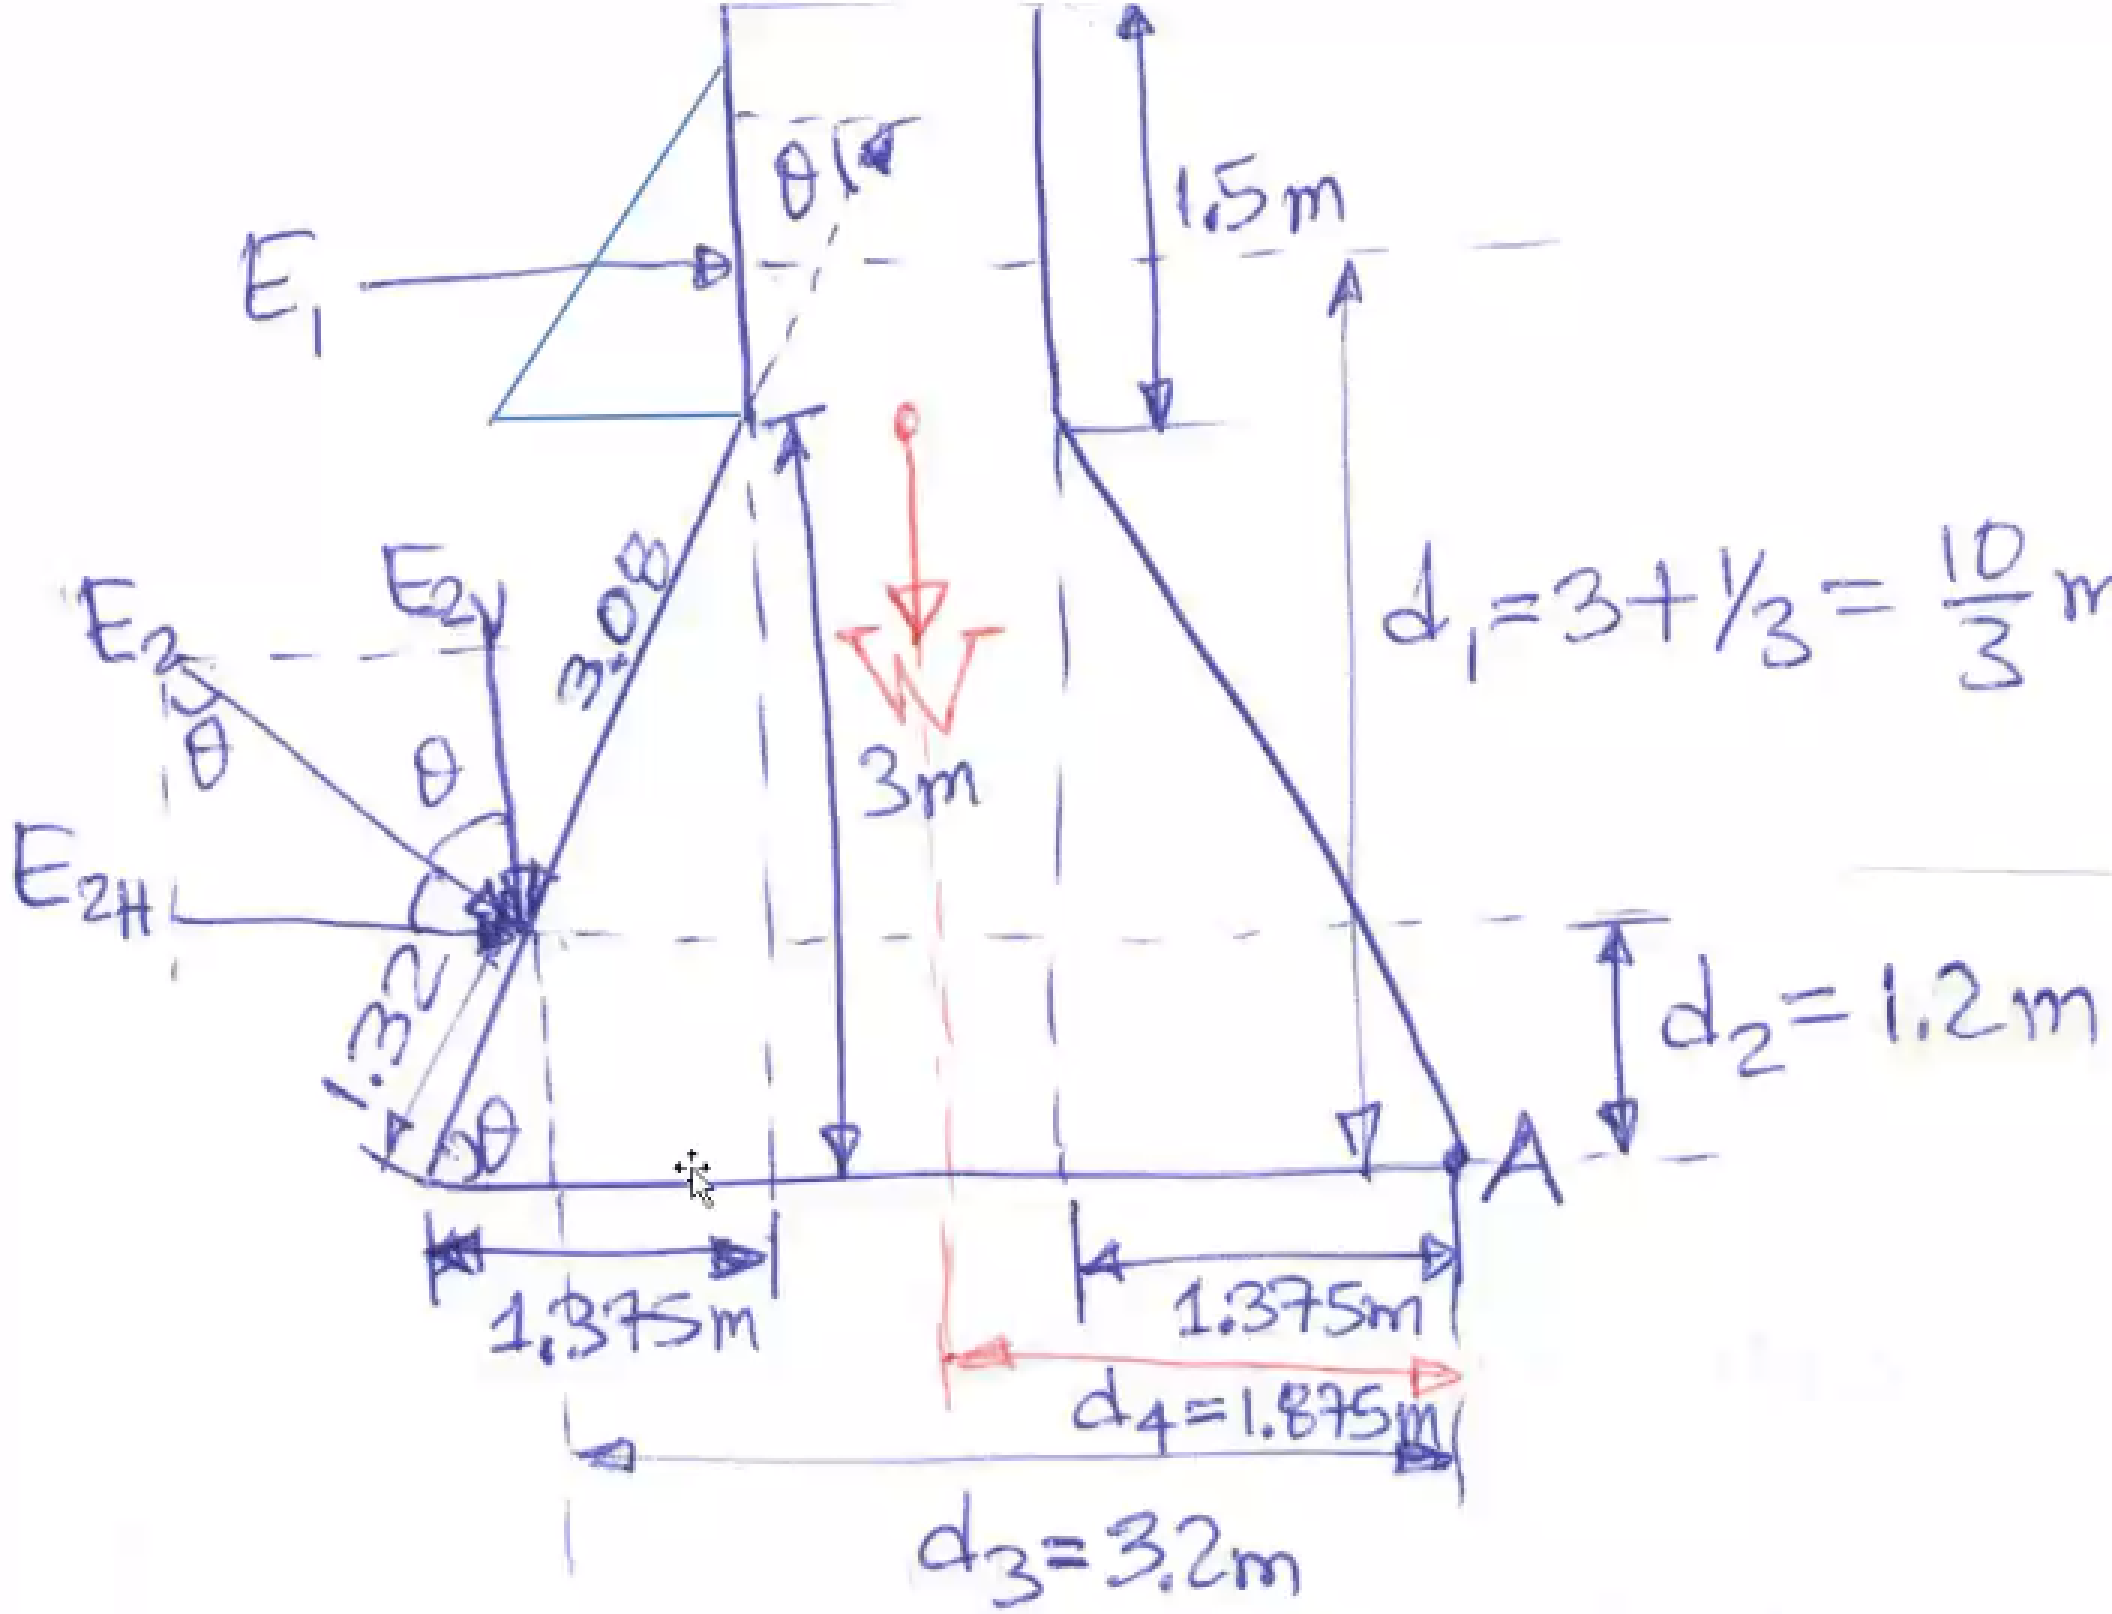
\includegraphics[width=0.5\textwidth]{hb20.png}
  \caption{Diagrama de Fuerzas}
  \label{hb20}
\end{figure}

\begin{problem}
    Determine la magnitud de la fuerza $P$ es necesaria para mantener la compuerta triangular en la posición mostrada en la figura
\end{problem}

\begin{figure}[h!]
\centering
  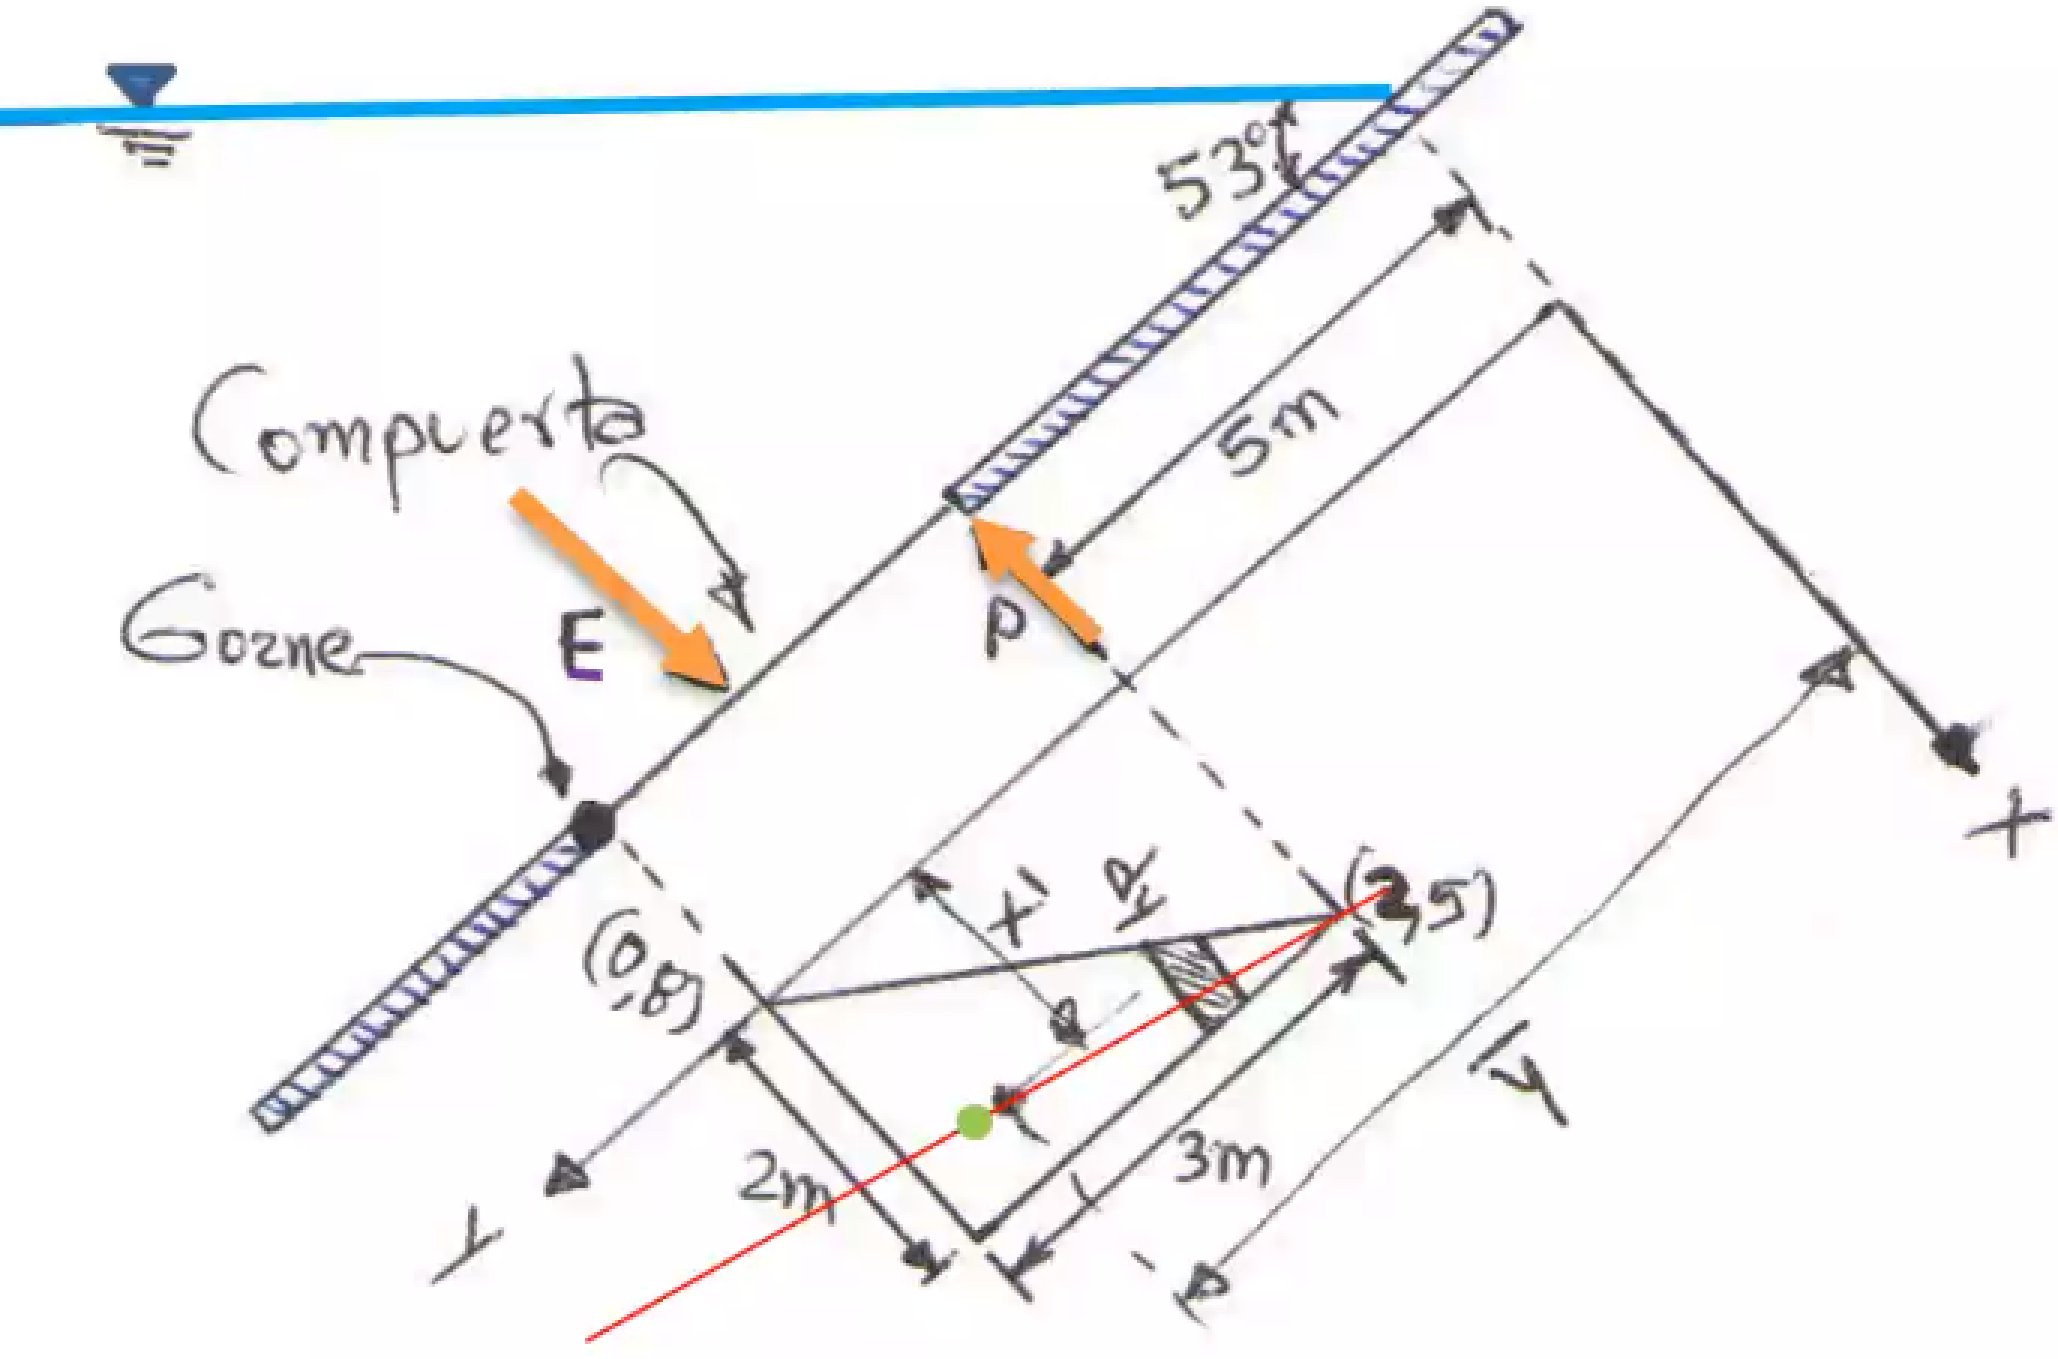
\includegraphics[width=0.5\textwidth]{hb21.png}
  \caption{Esquema del problema}
  \label{hb21}
\end{figure}

\textit{ Sol. }

Se tienen los siguientes datos:
\begin{align*}
    &\bar{y}=7m&&\bar{x}=\frac{4}{3}m&&P_1:(0,8)\\
    &P_2:(2,5)&&x=my+z&&P_1:0=m(8)+z&&P_2:2=m(5)+z
\end{align*}

Se obtiene mediante álgebra, la ecuación de la recta diagonal de la compuerta y es: 
\begin{align*}
    &y=-\frac{3}{2}x+8&&x=\frac{2}{3}(8-y)
\end{align*}

El empuje sobre la compuerta es:
    \begin{align*}
        &E=\int p\, dA=\int \omega\sin{(\alpha)}y\, dA\int_5^8y(2-x)\, dy\\
        &E=\frac{2}{3}\omega\sin{(\alpha)}\left\lceil \frac{y^3}{3}-5\frac{y^2}{2}\right\rceil_5^8=16.771ton
    \end{align*}
Las coordenadas del centro de presión donde está actuando el empuje se obtienen
\begin{equation*}
    y_{cp}=\bar{y}+\frac{\bar{I}_x}{\bar{y}A}=\frac{\frac{bh^3}{36}}{\frac{bh}{2}\bar{y}}=7m+\frac{\frac{2m\cdot (3m)^3}{36}}{\frac{(2m)(3m)}{2}7m}=7.0714m
\end{equation*}
La abscisa no se necesita pero se obtiene:
\begin{equation*}
    x_{cp}=\bar{x}+\frac{\bar{I}_{xy}}{\bar{y}A}=\frac{4}{3}+\frac{-\frac{(2m)^2(3m)^2}{72}}{(3m^2)(7m)}=1.3095m
\end{equation*}
En el gozne (articulación, bisagra) como puede girar libremente, la sumatoria de momentos es cero así:
\begin{align*}
    &\alpha P=dE\\
    &p=\frac{dE}{\alpha}=\frac{(8m-7.0714m)(16.771ton)}{3m}=5.191ton
\end{align*}

\subsection{Superficies Curvas}

\begin{figure}[h!]
\centering
  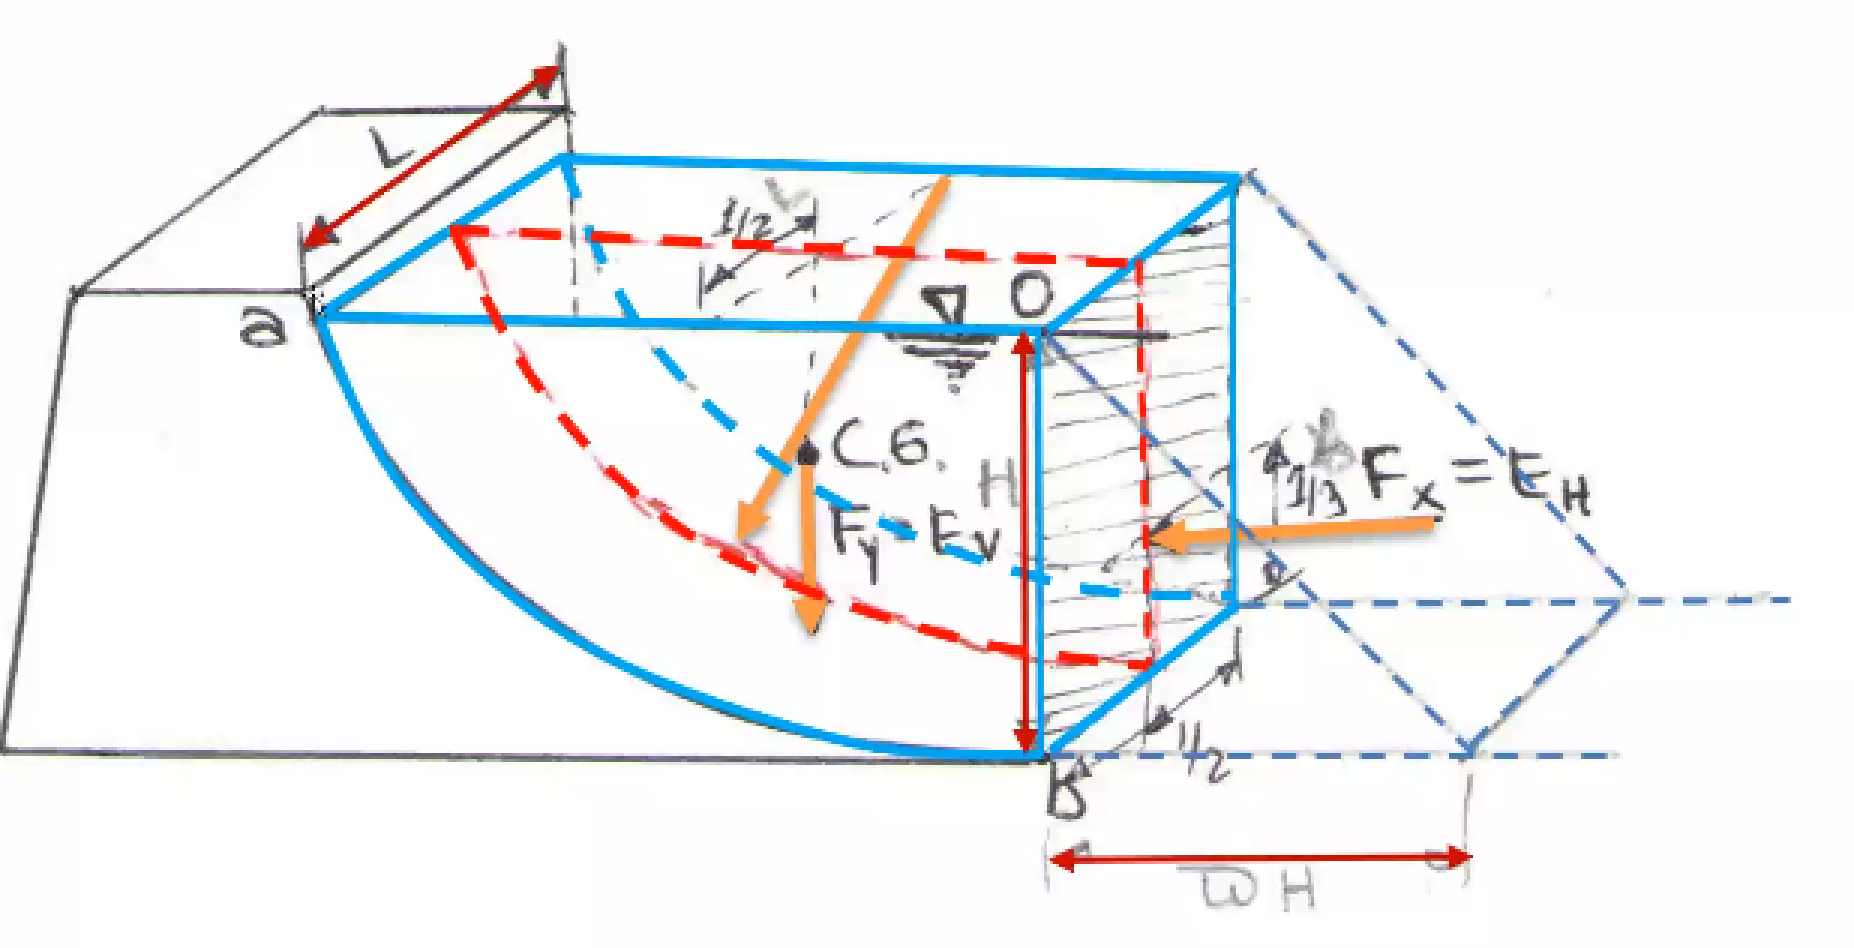
\includegraphics[width=0.5\textwidth]{hb22.png}
  \caption{Esquemas del problema}
  \label{hb22}
\end{figure}

Considerando las fuerzas que actúan sobre el prisma líquido ilustrado en la figura, limitado por la superficie libre $ao$ por la superficie vertical $ob$ y por la superficie curva $ab$. El peso de este volumen es una fuerza $W$, vertical hacia abajo, y la reacción del resto del líquido del prisma considerado, es una fuerza horizontal ($F_x$), actuando de derecha a izquierda sobre $ob$.
Estas fuerzas $F_x,W$ se mantienen en equilibrio al existir fuerzas iguales y opuestas de reacción de superficie curva $ab$. Se deduce que la componente horizontal $F_x$ de empuje pasando por su centro de gravedad: 
\begin{figure}[h!]
    \centering
      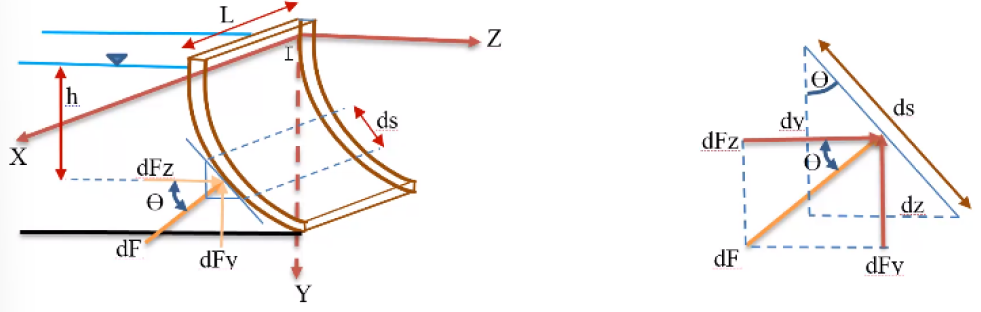
\includegraphics[width=0.5\textwidth]{hb23.png}
      \caption{Diagrama de fuerzas}
      \label{hb23}
    \end{figure}
Para el empuje horizontal: 
\begin{align*}
    &dF_z=dF\cos\theta=pdA\cos\theta=\omega hLdS\cos\theta=\omega Ldt=p\, dA_y\\ 
    &\int dF_z=E_H=\int p\, DA_y
\end{align*}
Así el empuje hidráulico horizontal es el empuje sobre la proyección vertical de la superficie curva. Para el empuje vertical:
\begin{align*}
    &dF_y=df\sin\theta=psA\sin\theta=\omega hLds\sin\theta=\omega hdzL=\omega\,dV=dW_a\\
    &\int_A dF_y=\int dW\\
    &Ev=W
\end{align*}

\begin{problem}[Calcule la fuerza P]
    necesaria para detener la compuerta de 4m de ancho en la posición mostrada en la figura \ref{hb24}. Omita el peso de la compuerta.
\end{problem}
\begin{figure}[h!]
\centering
  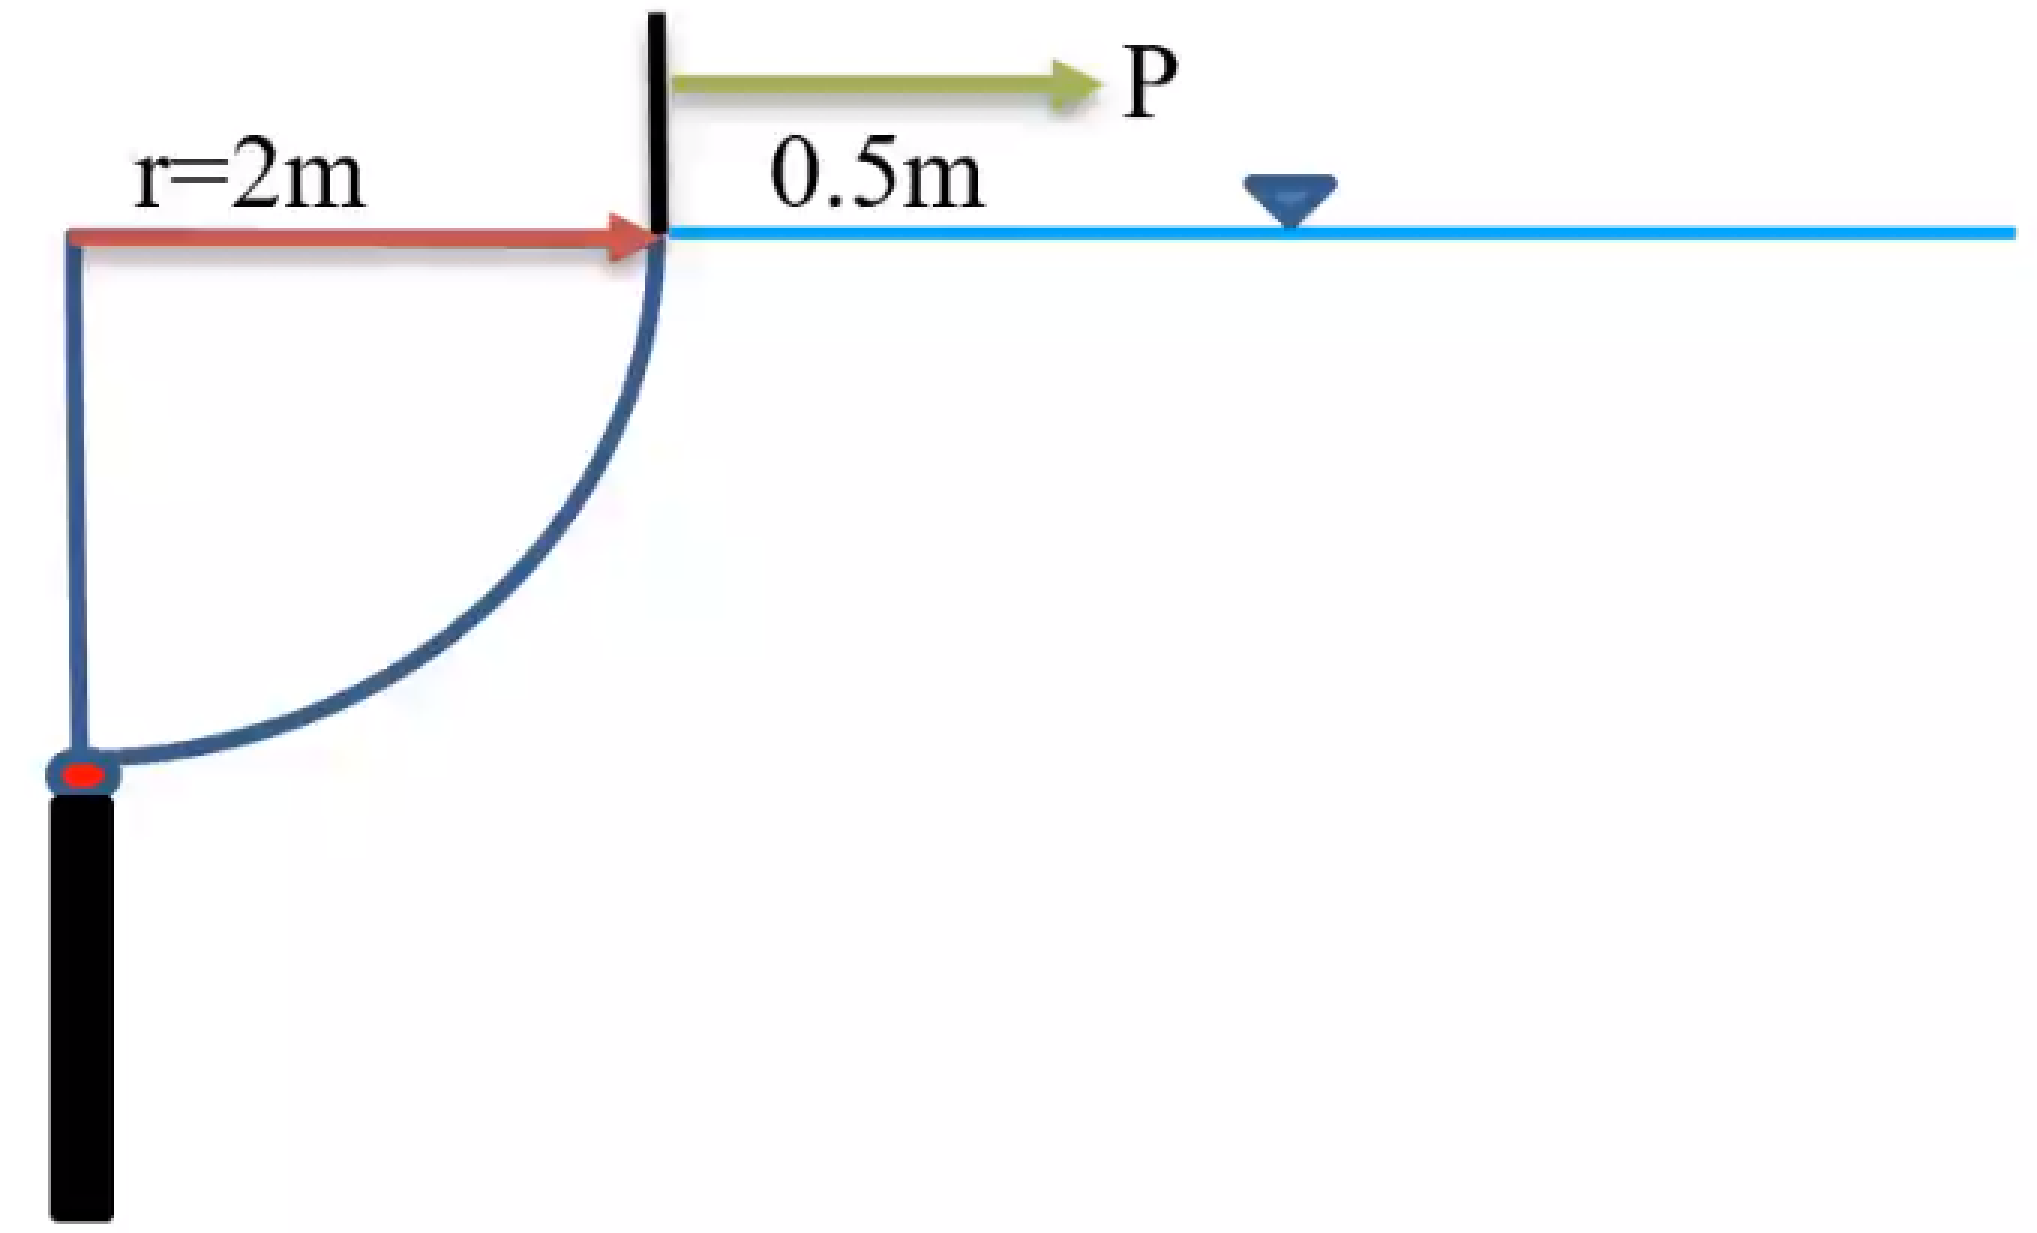
\includegraphics[width=0.5\textwidth]{hb24.png}
  \caption{Compuerta}
  \label{hb24}
\end{figure}

\textit{ Sol. }

\begin{figure}[h!]
\centering
  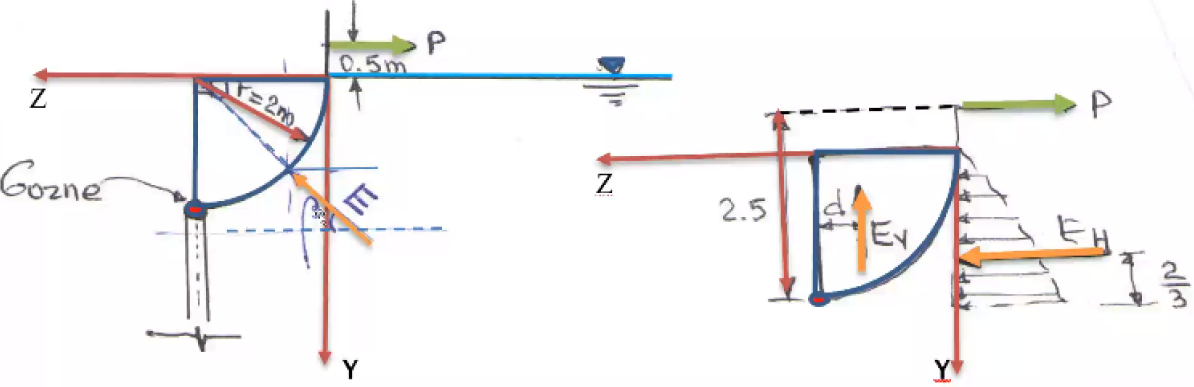
\includegraphics[width=0.5\textwidth]{hb25.png}
  \caption{Diagrama de fuerzas en la compuerta}
  \label{hb35}
\end{figure}
\begin{align*}
    &E_H=\bar{\omega}\bar{h}A=\bar{\omega}\frac{r}{2}br=1,000\frac{kg}{m^3}\cdot\frac{2m}{2}4m\cdot 2m=8\,ton\\
    &E_H=\bar{\omega}V=\bar{\omega}Ab=\bar{\omega}frac{\pi r^2}{4}b=1,000\frac{kg}{m^3}\cdot\frac{\pi\cdot (2m)^2}{4}\cdot 4m=12.566\,ton\\
    &E=\sqrt{E_h^2+E^2_v}=\sqrt{(8\,ton)^2+(12.566\,ton)^2}=14.896\,ton\\
    &d=\frac{4r}{3\pi}=0.8488m\\
    &\beta=\arctan{\frac{E_v}{E_H}}=57.518^{\circ}\\
    &Prof.c.p.=r\sin{(\beta)}=2r\sin{(57.518)}=1.687m
\end{align*}

Como la sumatoria de momentos en la articulación es igual a cero: 
\begin{align*}
    &\sum_A =(r+0.5M)p-\frac{2}{3}E_H-dE_v=0\\
    &P=\frac{\frac{2}{3}\cdot 8+0.8488(12.566)}{2.5}=6.5\, ton
\end{align*}

\begin{problem}[Determine las características vectoriales]
    del empuje sobre la compuerta de 2.5m de ancho, radio de 2m y ángulo $\theta=85^{\circ}$.
\end{problem}
\begin{figure}[h!]
\centering
  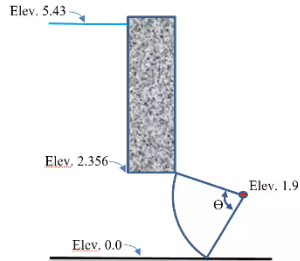
\includegraphics[width=0.5\textwidth]{hb26.png}
  \caption{Compuerta, esquema del problema}
  \label{hb26}
\end{figure}

\textit{ Sol. }

\begin{figure}[h!]
\centering
  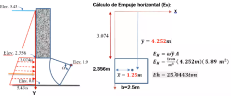
\includegraphics[width=0.5\textwidth]{hb27.png}
  \caption{Diagrama de fuerzas de empuje horizontal}
  \label{hb27}
\end{figure}

\begin{figure}[h!]
\centering
  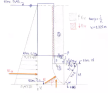
\includegraphics[width=0.5\textwidth]{hb28.png}
  \caption{Cálculo de empuje vertical}
  \label{hb28}
\end{figure}

Para el cálculo de los ángulos, es fácil deducir que: 
\begin{align*}
    &\tan{(\beta)}=\frac{j}{k}\implies k=1.322m\\ 
    &Z=2\sin{(\beta)}=0.4565\\
    &k=z-x=0.31\\
    &\alpha=71.8^{\circ}=13.195\implies x=0.1463
\end{align*}
\begin{align*}
    &E_v=V\omega=\left(A_1+A_2+A_3\right)b\omega\\
    &A_1=ka=1.322(5.43-2.356)=4.064m^2\\
    &A_2=\frac{kj}{2}=1.322\cdot \frac{0.31}{2}=0.2049m^2\\
    &A_3=\pi r^2\left(\frac{\theta}{360}\right)-A^{\prime}\implies A^{\prime}=\frac{(x+1.9)0.6245}{2}=0.63896m^2\\
    &A_3=\pi 2^2\left(\frac{85}{360}\right)-0.63896=2.3281m^2\\ 
    &E_v=\left(4.064+0.2049+2.3281\right)2.5m\cdot \frac{1\,ton}{m^3}=16.493\,ton\\
    &E=\sqrt{E_H^2+E_v^2}=\sqrt{(25.0443\,ton)^2+(16.493\,ton)^2}=29.987\,ton\\
    &\beta^{\prime}=\sqrt{\left(\frac{E_v}{E_H}\right)}=\arctan{\left(\frac{16.493}{25.443}\right)}=33.36^{\circ}\\
    &Elev.c.p. =elev.perno-r\sin{(\beta^{\prime})}=1.9-2\cdot \sin{(33.36)}=0.8m
\end{align*}

\subsection{Principio de flotación de Arquímides}

Para un cuerpo parcial o totalmente sumergido en un líquido en reposo (relativo), existe una fuerza de flotación (vertical hacia arriba) cuya magnitud es el peso del líquido desalojado, y pasa por el centro de gravedad del volumen desalojado.

\begin{figure}[h!]
    \centering
      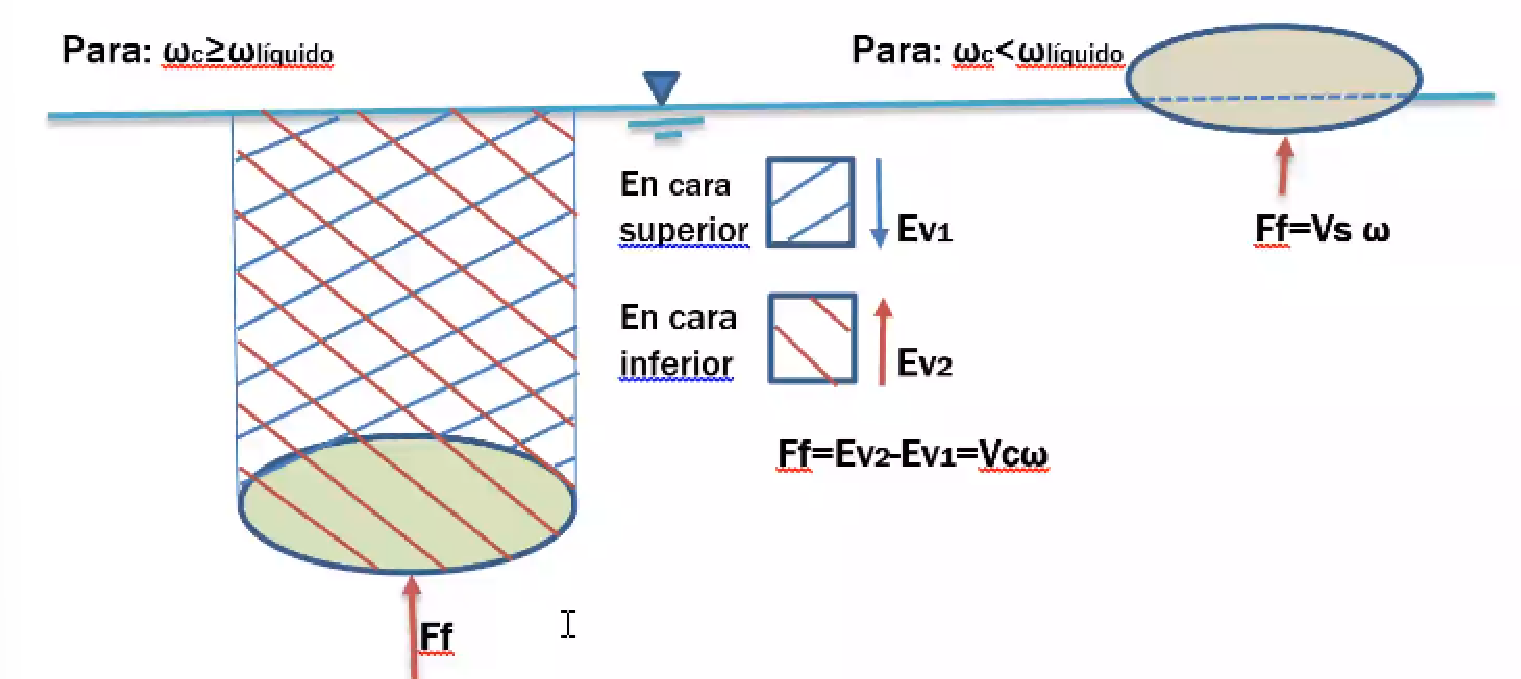
\includegraphics[width=0.5\textwidth]{hb48.pdf}
      \caption{Principio de Arquímedes}
      \label{hb48}
\end{figure}

\begin{problem}[Una pieza de aluminio (s)=2.7]
    cuelga de un bloque de plástico (s=0.53). La pieza metálica tiene un volumen de $3335cm^3$. Determine la tensión en el cable, y ¿Cuánto se sumerge el bloque de plástico en el agua?
\end{problem}

\begin{figure}[h!]
\centering
  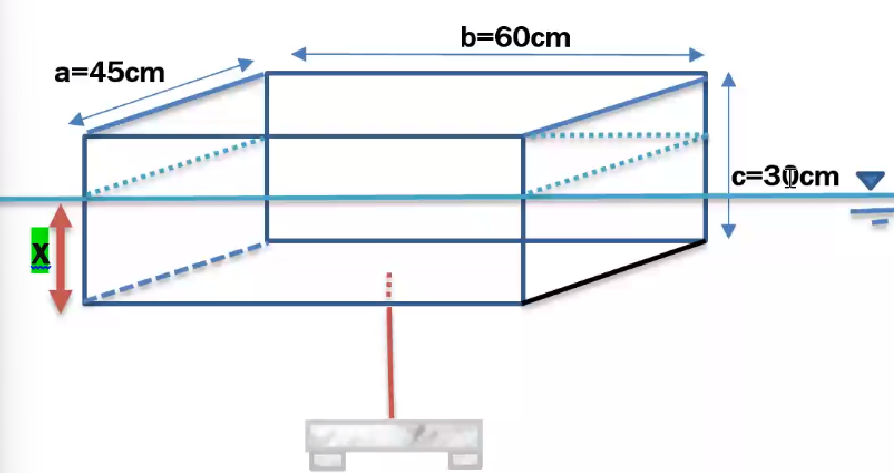
\includegraphics[width=0.5\textwidth]{hb49.pdf}
  \caption{Pieza de aluminio y bloque de plástico}
  \label{hb49}
\end{figure}

\textit{ Sol. }

DCL 1 de la pieza de metal: debe cumplirse que $\sum F_y=0$, por lo que se aplica $T+F_f=W$, así la tensión en el cable será:
\begin{align*}
    &T=W-F_f=V_{al}\omega_{al}-V_{al}\omega=V_{al}\left(\omega_{al}-\omega\right)\\
    &T=0.003335m^3\left(2700-1,000\right)\frac{kg}{m^3}=5.67kg
\end{align*}

DCL 2 del bloque de plástico: Debe cumplirse nuevamente que $\sum F_y=0$, así 
\begin{align*}
    &F_f=W+T=V_{pl}\omega_{pl}+T=V_{s\omega}=abx\omega\\
    &x=\frac{V_{pl}\omega_{pl}+T}{ab\omega}=\frac{0.3\cdot 0.45\cdot 0.6m^3\cdot 530\frac{kg}{m^3}+5.67kg}{0.45\cdot 0.6m^21,000\frac{kg}{m^3}}=0.18m
\end{align*}

\begin{problem}[La boya de plástico (s=0.62)]
    y la esfera suspendida es metálica de $S=4.3$. La altura del cono es de 30cm. Determine el volumen, peso y radio de la esfera que cuelga del cono, de tal manera que sólo la mitad del volumen de la semiesfera sea el que sobresalga del nivel del mar. Determine también el valor de $x$ y la tensión del cable
\end{problem}

\begin{figure}[h!]
\centering
  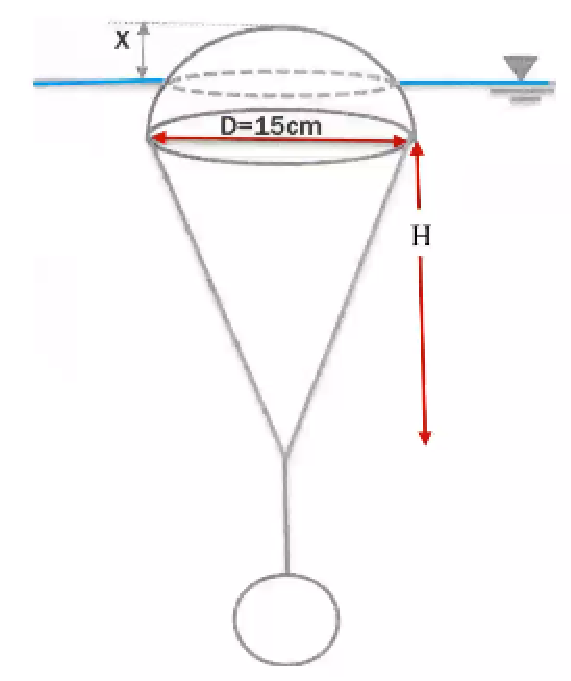
\includegraphics[width=0.5\textwidth]{hb40.pdf}
  \caption{Esquema del problema}
  \label{hb40}
\end{figure}

\textit{ Sol. }

El volumen del cono es:
\begin{equation*}
    V_c=\frac{\pi D^2h}{12}=\frac{\pi(0.15m)^20.3m}{12}=0.00176715m^3
\end{equation*}
El volumen de la semiesfera es: 
\begin{equation*}
    V_{se}=\frac{2\pi r^3}{3}=\frac{2\pi(0.075m)^3}{3}=8.836\times 10^{-4}m^3
\end{equation*}
EL volumen del casquete que sobresale del agua, es la mitad de la semiesfera: $V_c=4.418\times 10^{-4}m^3$.
La fórmula del volumen de un casquete se obtiene:
\begin{align*}
    &dV=\pi a^2\,dx\implies a^2=r^2-\left(r-x\right)^2\\
    &a^2=2rx-x^2\implies \int_0^x\pi\left(2rx-x^2\right)\,dx\\
    &V=\frac{\pi x^2}{3}\left(3r-x\right)
\end{align*}
Si se tiene el volumen del casquete: la fórmula anterior nos resuelve la altura del casquete que es $x$, la cual se puede resolver por iteraciones o por algún método numérico más eficiente.

\begin{equation*}
    V_c=\frac{\pi x^2}{3}(3r-x)=4.418\times 10^{-4}m^3
\end{equation*}
La solución es $x=0.04896m$, prácticamente 4.9cm

DCL1 del cono y semiesfera:
\begin{align*}
    &F_f=T+W\\
    &T=F-F-W=\left(V_s.ca.+V_{co}\right)\omega^{\prime}-\left(V_{sem}.es.+V_{co}\right)\omega_p\\
    &T=\left(4.418\times 10{-3}\right)m^3\left(620\frac{kg}{m^3}\right)\\
    &T=2.264-1.6434=0.6206kg
\end{align*}

DCL2 de la esfera metálica:
\begin{align*}
    &V_e=\frac{T}{\left(\omega_m-\omega^{\prime}\right)}=\frac{0.6206kg}{4300\frac{kg}{m^3}-1025\frac{kg}{m^3}}=1.895\times 10^{-04}m^3\\
    &r=\left(3V_e/4\pi\right)^{\frac{1}{3}}=0.0356m\\
    &W_e=V_{\omega m}=1.895\times 10^{-04}m^3\left(\frac{4300kg}{m^3}\right)=0.815kg
\end{align*}

\section{Hidrodinámica}

Esta rama de la mecánica de fluidos se ocupa de las leyes de los fluidos en movimiento; estas leyes son enormemente complejas, y aunque la hidrodinámica tiene una importancia práctica mayor que la hidrostática, sólo podemos tratar aquí algunos conceptos básicos.

El interés por la hidrodinámica se remonta a las aplicaciones más antiguas de los fluidos en ingeniería. Arquímedes (250 A. C.) realizó una de las primeras contribuciones con la invención, que se le atribuye tradicionalmente, del tornillo sin fin. La acción impulsora del tornillo de Arquimedes es similar a la de la pieza semejante a un sacacorchos que tienen las picadoras de carne manuales. Los romanos desarrollaron otras máquinas y mecanismos hidráulicos; no sólo empleaban el tornillo de Arquimedes para bombear agua en agricultura y minería, sino que también construyeron extensos sistemas de acueductos, algunos de los cuales todavía funcionan. En el siglo I a.C., el arquitecto e ingeniero romano Marco Vitrubio Polio inventó la rueda hidráulica horizontal, con lo que revolucionó la técnica de moler grano.

\begin{definition}[Corriente líquida]
Es el desplazamiento en una dirección determinada de una masa líquida.
\end{definition}
Algunas finalidades del estudio de corrientes líquidas son por ejemplo: Riego, generación de energía eléctrica mediante motores hidráulicos, abastecimiento de agua (Doméstico, industrial, agrícola, pecuario, recreativo, etc.), drenaje de agua (agrícola, pluvial, de asentamientos humanos, de la industria), etc.
Como elementos técnicos inherentes a corrientes líquidas, principalmente de agua, se consideran: gasto, velocidad, área hidráulica, perímetro mojado, radio hidráulico, tirante, no. De Reynolds, de Froude (y otros) gradiente hidráulico, línea de energía, línea piezométrica energía hidráulica, potencia hidráulica, presión hidrodinámica.
\begin{definition}[Trayectoria]
    Es el lugar geométrico de las posiciones de una misma partícula, al transcurrir el tiempo.
\end{definition}
\begin{definition}[Línea de corriente]
    Es una curva imaginaria, en donde en cada uno de sus puntos tiene por tangente al segmento dirigido que representa la velocidad en dicho punto para un tiempo considerado. En general las líneas de corriente varían con el tiempo, pueden ser convergentes, divergentes o paralelas, pero nunca cortarse. En el caso del movimiento permanente, las líneas de corriente son fijas y coinciden con las trayectorias.
\end{definition}

\begin{definition}[Tubo de corriente]
    Es la región parcial de flujo líquido que se encuentra delimitado por una familia de línea de corriente
\end{definition}

\subsection{Tipos de movimiento en las corrientes líquidas}

¿Cómo se mueven las partículas de agua?

\begin{enumerate}
    \item \textbf{Movimiento laminar:} Las partículas al moverse, describen trayectorias paralelas, su número de Reynolds $(RE)\leq 2,000$, sus pérdidas de energía por recorrido son función lineal de la velocidad y el diagrama de velocidades es parabólico, véase la figura \ref{hb41} 
    \item \textbf{Movimiento turbulento:} Las partículas líquidas al moverse describen trayectorias sinuosas en el espacio, su número de Reynolds es $\geq 24,000$, sus pérdidas de energía por recorrido son función cuadrática de la velocidad de ellas y el diagrama de velocidades es aproximadamente rectangular, véase la figura \ref{hb42}.
    \item \textbf{Movimiento transicional:} Para $Re$ entre 2,000 y 4,000, también llamada zona crítica, véase la figura \ref{hb43} 
\end{enumerate}

\begin{figure}[h!]
\centering
    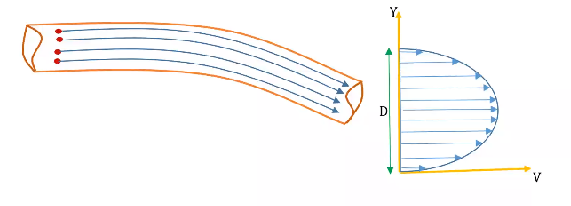
\includegraphics[width=0.5\textwidth]{hb41.pdf}
    \caption{Movimiento laminar}
    \label{hb41}
\end{figure}
\begin{figure}[h!]
\centering
    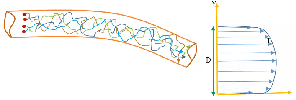
\includegraphics[width=0.5\textwidth]{hb42.pdf}
    \caption{Movimiento turbulento}
    \label{hb42}
\end{figure}
\begin{figure}[h!]
    \centering
        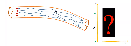
\includegraphics[width=0.5\textwidth]{hb43.pdf}
        \caption{Movimiento transicional}
        \label{hb43}
\end{figure}
Ecuación de continuidad para una corriente líquida (Principio de conservación de masa)

El principio de conservación de masa establece que, la cantidad neta de masa que atraviesa una superficie de control en la unidad de tiempo más la rapidez de variación de masa contenida en el volumen es igual a cero.

Sea el tubo de corriente de fluido compresible de la figura, con frontera sólida, donde V es la velocidad media representativa de la sección y S es el eje del tubo (coordenada curvilínea).

\begin{figure}[h!]
    \centering
        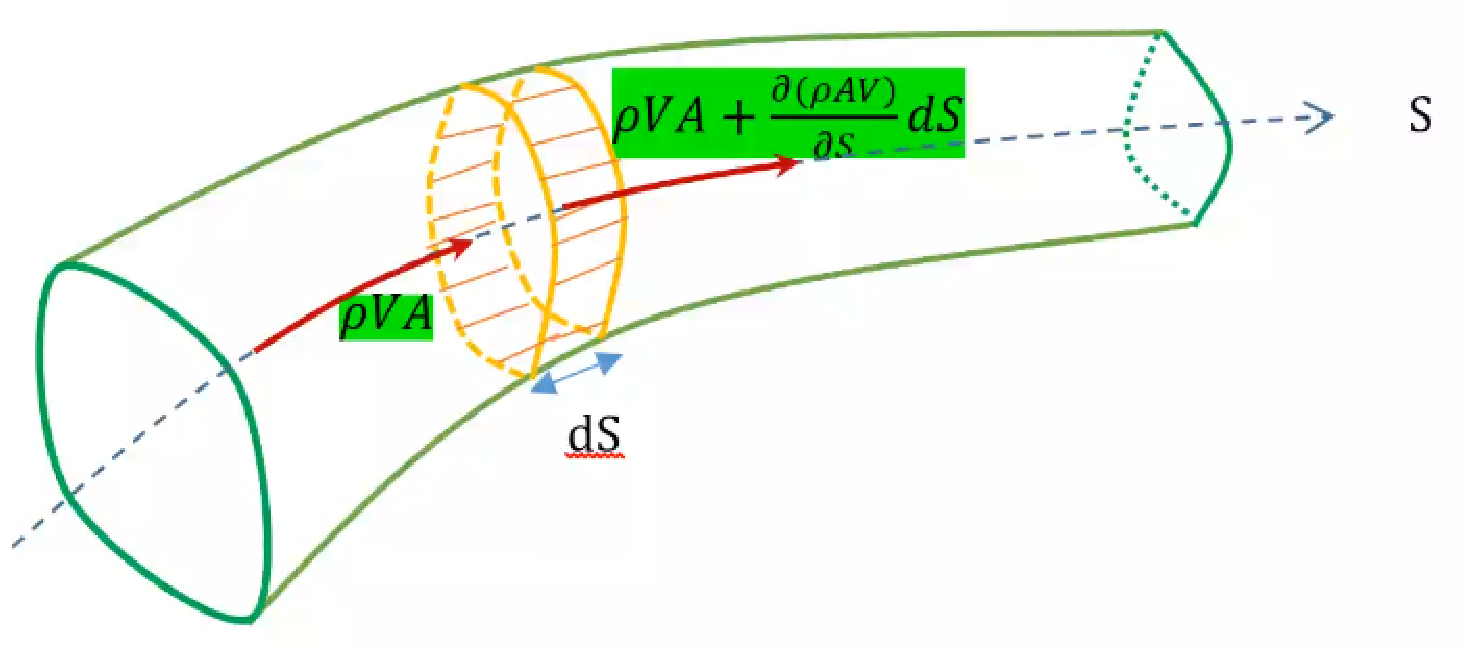
\includegraphics[width=0.5\textwidth]{hb44.pdf}
        \caption{Tubo de corriente}
    \label{hb44}
\end{figure}

La cantidad de masa neta por unidad de tiempo que atraviesa la frontera de control es: 
\begin{equation}
    \left(\rho VA+\frac{\partial (\rho AV)}{\rho S}\, dS\right)-\rho VA=\frac{\partial (\rho AV)}{\rho S}\,dS
\end{equation}
La rapidez con que varía la masa dentro del volumen de control por unidad de tiempo es: 
\begin{equation}
    \frac{\partial \left(\rho AdS\right)}{\partial t}
\end{equation}
Así:
\begin{equation*}
    \frac{\partial (\rho AV)}{\partial S}\,dS+\frac{\partial (\rho AdS)}{\partial t}=0
\end{equation*}
Como $dS$ no es función del tiempo:
\begin{equation*}
    \frac{\partial (\rho AV)}{\partial S}+\frac{\partial (\rho A)}{\partial t}=0
\end{equation*}
Para escurrimiento permanente o establecido las derivadas con respecto al tiempo son nulas.
\begin{equation}
    \frac{\partial (\rho AV)}{\partial S}=0
\end{equation}
Lo que implica que el producto $VA$ es constante en cualquier sección del tubo de corriente y es $VA=Q$ (gasto). Cuando una corriente mantiene constante su gasto en un tramo, se dice que la corriente es continua en éste, y se cumplirá:
\begin{align*}
    &Q=Q_1=Q_2=Q_n\\
    &A_1V_1=A_2V_2=A_nV_n
\end{align*}

\subsection{Elementos de la sección transversal de una corriente}
Las secciones transversales de una corriente pueden ser naturales o artificiales. Las secciones naturales por lo general son irregulares. En las secciones artificiales la sección se construye con forma geométrica, pudiendo ser de conducto cerrado o abierto.
\begin{figure}[h!]
\centering
  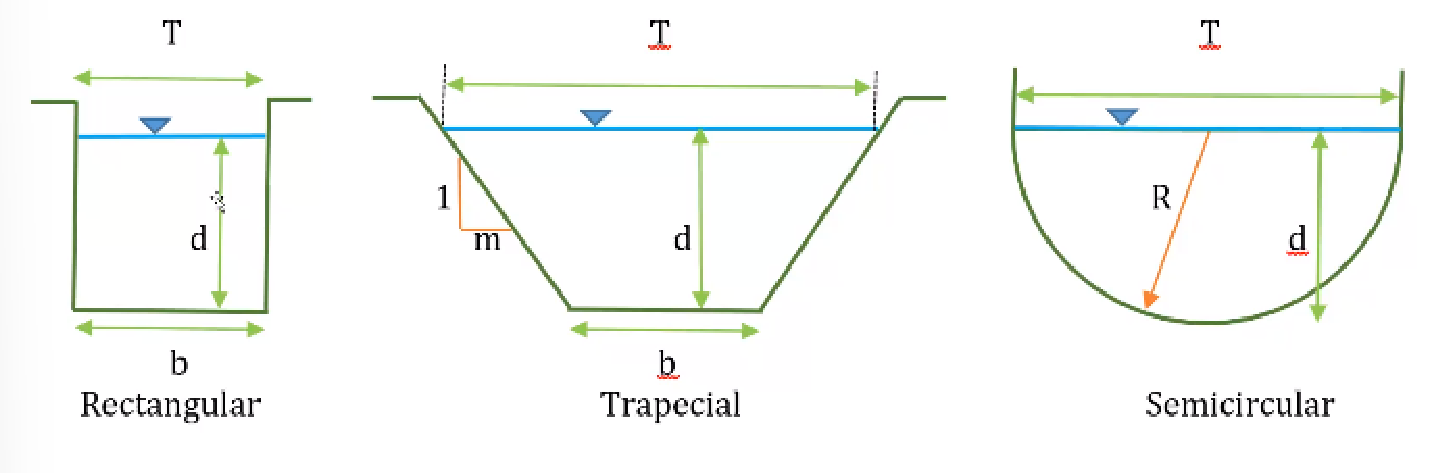
\includegraphics[width=0.5\textwidth]{hb45.pdf}
  \caption{Secciones de conducto abierto}
  \label{hb45}
\end{figure}
\begin{figure}[h!]
    \centering
      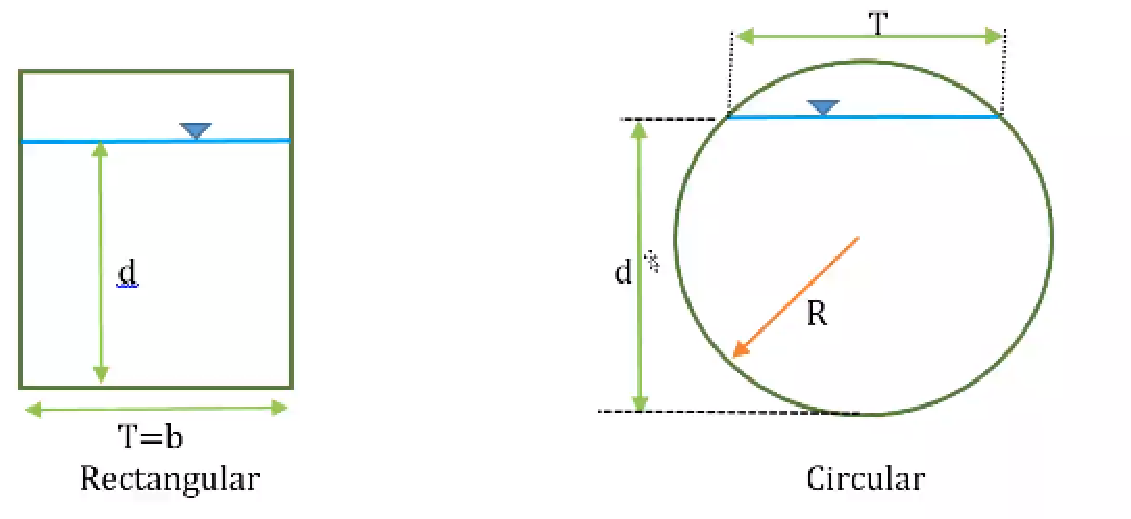
\includegraphics[width=0.5\textwidth]{hb46.pdf}
      \caption{secciones de conducto cerrado}
      \label{hb46}
    \end{figure}
Los principales elementos de la sección transversal de una corriente a superficie libre son:
\begin{itemize}
    \item \textbf{Tirante $d$.} Es la máxima distancia al piso del cauce a la superficie libre del agua (SLA)
    \item \textbf{Área hidráulica $A$.} Es la superficie de la sección transversal a la corriente
    \item \textbf{Ancho de la superficie libre del agua $T$.} Es la longitud de la lámina en la superficie libre del agua, en la sección transversal de la corriente
    \item \textbf{Perímetro mojado $P$.} Es la longitud del contacto de la corriente y la pared del conducto
    \item \textbf{Radio hidráulico $R$.} Es el cociente del área hidráulica y el perímetro mojado.
\end{itemize}

Para una sección trapecial, sus elementos se determinan por la semejanza de triángulos y elementos:
\begin{align*}
    &X=md
    &A=bd+md^2\\
    &T=2md+b\\
    &P=b+2d\sqrt{1+m^2}\\
    &R=\frac{A}{P}=\frac{bd+md^2}{b+2d\sqrt{1+m^2}}
\end{align*}

\begin{problem}[Determine los elementos técnicos de sección trapecial]
\end{problem}
\begin{figure}[h!]
\centering
  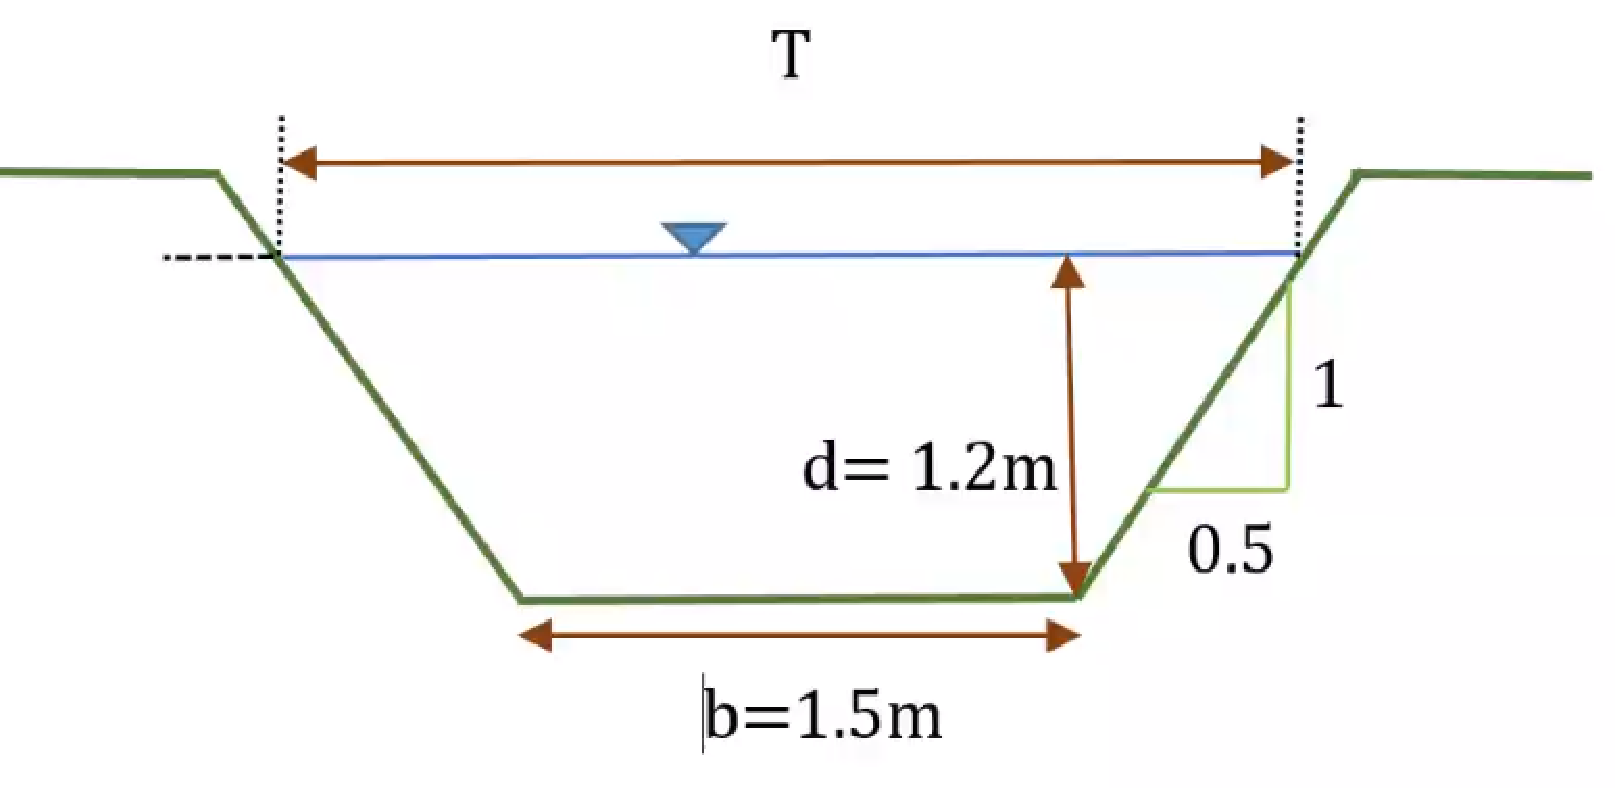
\includegraphics[width=0.5\textwidth]{hb50.pdf}
  \caption{Esquema del problema}
  \label{hb50}
\end{figure}
\textit{ Sol. }
\begin{align*}
    &T=b+2md=1.5+2(0.5)(1.2m)=\frac{6 m}{5} + \frac{3}{2}=2.7m\\
    &A=bd+md^2=1.2(1.5m)+0.5(1.2m)^2=2.52m^2\\
    &P=b+2d\sqrt{1+m^2}=1.5m+2(1.2m)\sqrt{1+0.5^2}=4.183m\\
    &R=\frac{2.52m^2}{4.183m}=0.60m
\end{align*}

\begin{example}
    Para una sección circular
\end{example}
\begin{figure}[h!]
\centering
  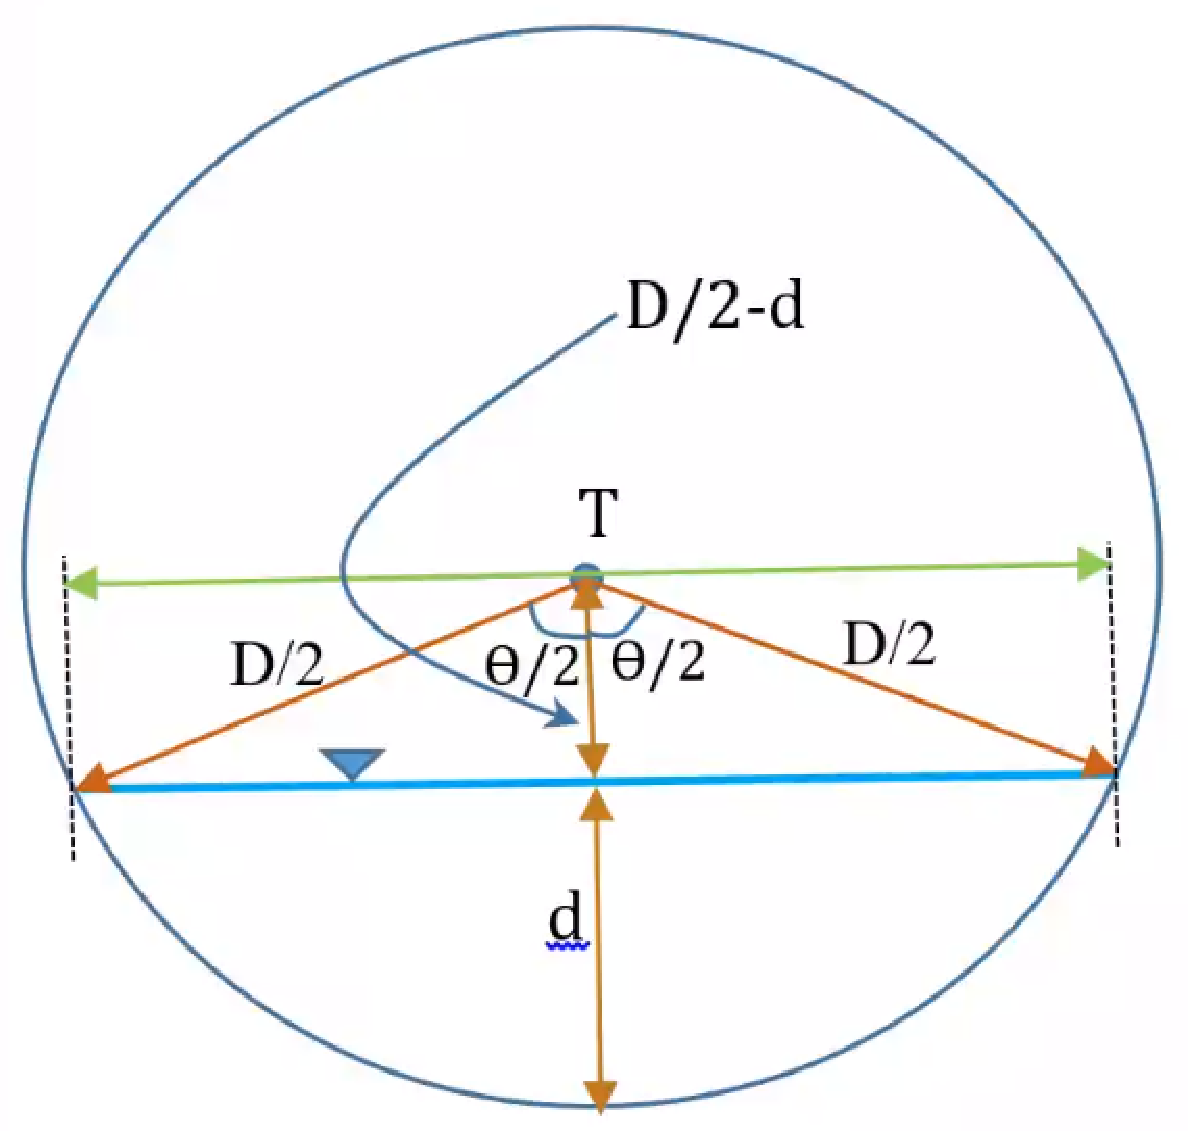
\includegraphics[width=0.5\textwidth]{hb51.pdf}
  \caption{Sección circular}
  \label{hb51}
\end{figure}
\begin{align*}
    &d=\frac{D}{2}-\frac{D}{2}\cos{\left(\frac{\theta}{2}\right)}=\frac{D}{2}\left(1-\cos{\left(\frac{\theta}{2}\right)}\right)\\
    &\theta=2\arccos{\left(1-\frac{2d}{D}\right)}\\
    &T=2\frac{D}{2}\sin{\left(\frac{\theta}{2}\right)}=D\left(\sin{\left(\frac{\theta}{2}\right)}\right)\\
    &\left(\frac{T}{2}\right)^2=\left(\frac{D}{2}\right)^2-\left(\frac{D}{2}-d\right)^2\\
    &T=2\sqrt{d(D-d)}\\
    &P=\pi D\frac{\theta}{360}\\
    &A=\pi\frac{D^2}{4}-\frac{\frac{D}{2}\sin{\left(\frac{\theta}{2}\right)}\frac{D}{2}\cos{\left(\frac{D}{2}\right)}}{2}=\\
    &\frac{D^2}{8}\left(\frac{\pi \theta}{180}\right)-\frac{D^2}{8}\sin{(\theta)}=\\
    &\text{Por identidad: }\, \sin{\left(\frac{\theta}{2}\right)}\cos{\left(\frac{\theta}{2}\right)}=\frac{1}{2}\sin{\left(2\frac{\theta}{2}\right)}=\frac{1}{2}\sin{(\theta)}\\ 
    &A=\frac{D^2}{8}\left(\frac{\pi\theta}{180}-\sin{(\theta)}\right)\\
    &R=\frac{A}{P}=\frac{\frac{D^2}{8}\left(\frac{\pi\theta}{180}-\sin{(\theta)}\right)}{\frac{D\cdot \pi\theta}{2\cdot 180}}=\frac{D}{4}\left(1-\frac{180}{\pi\theta}\sin{\theta}\right)
\end{align*}
\begin{equation}
    R=\frac{D}{4}\left(1-\frac{180}{\pi\theta}\sin{\theta}\right)
\end{equation}

\begin{problem}[Determine los elementos técnicos de la sección]
    $D=2m$ y $d=1.8m$
\end{problem}

\begin{figure}[h!]
\centering
  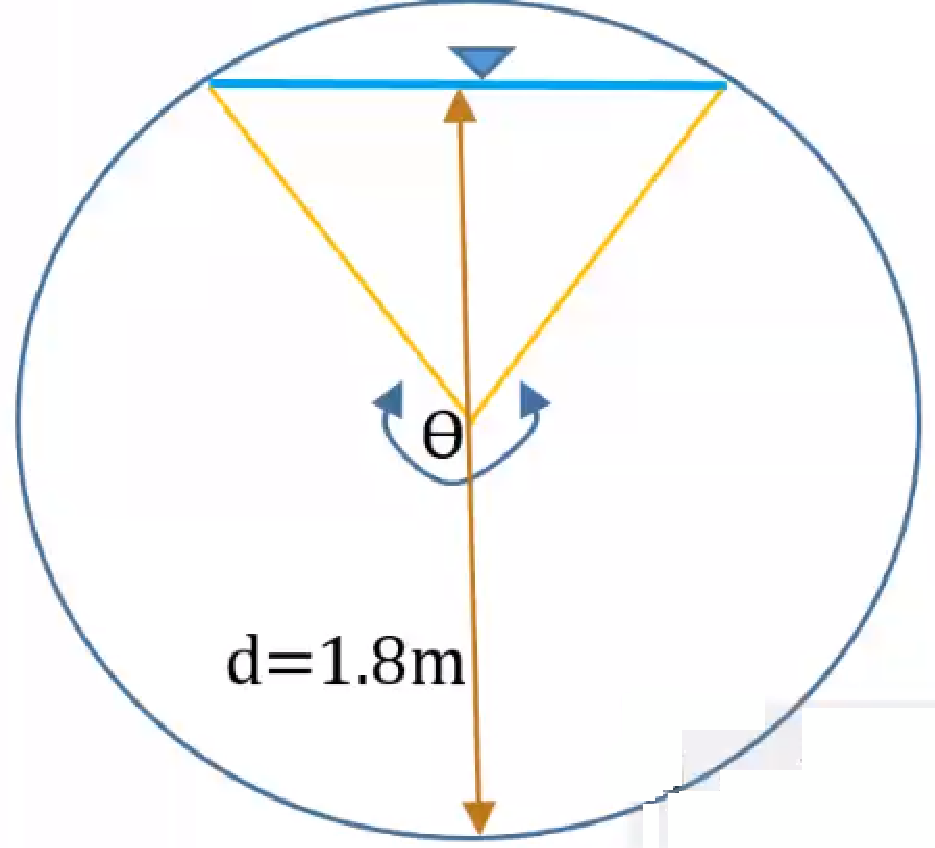
\includegraphics[width=0.5\textwidth]{hb52.pdf}
  \caption{Sección circular}
  \label{hb52}
\end{figure}
\textit{ Sol. }
\begin{align*}
    &\theta=2\arccos{\left(1-\frac{2d}{D}\right)}=2\arccos{\left(1-\frac{2(1.8)}{2}\right)}=286.26^{\circ}\\
    &T=2\sqrt{d(D-d)}=2\sqrt{(1.8)(2-1.8)}=1.2m\\
    &P=\pi D\frac{\theta}{360}=\pi\cdot 2\cdot\frac{286.26}{360}=4.9962m\\
    &A=\frac{2^2}{8}\left(\frac{\pi\cdot 286.26}{180}-\sin{(286.26)}\right)=2.9781m^2\\
    &R=\frac{D}{4}\left(1-\frac{180}{\pi\theta}\sin{\theta}\right)=\frac{2.9781}{4.9962}=0.5961m
\end{align*}

\subsection{Número de Reynolds}

El número de Reynolds ($Re$), es un parámetro adimensional que permite diferenciar el tipo de movimientos de partículas líquidas en corrientes, con lo cual se puede seleccionar la forma más adecuada de evaluación de pérdidas de carga por fricción, su fórmula nos determina la preponderancia de las fuerzas viscosas o de rozamiento sobre las de inercia.
\begin{equation*}
    Re =\frac{vD}{v} =\frac{vDp}{\mu}
\end{equation*}

En la que  $Re$ es número de Reynolds (adimensional), $v$ es la velocidad media del agua (m/s), $D$ es diámetro de la tubería ($m$), $p$ es la densidad $kg\cdot s(m^2)$ y $v$ viscosidad cinemática ($m^2/s$)

\begin{problem}[Determine las velocidades y el tipo de flujo en la tubería]
    que conduce un gasto de 0.4lps. El agua está a $29^{\circ}C$
\end{problem}
\begin{figure}[h!]
\centering
  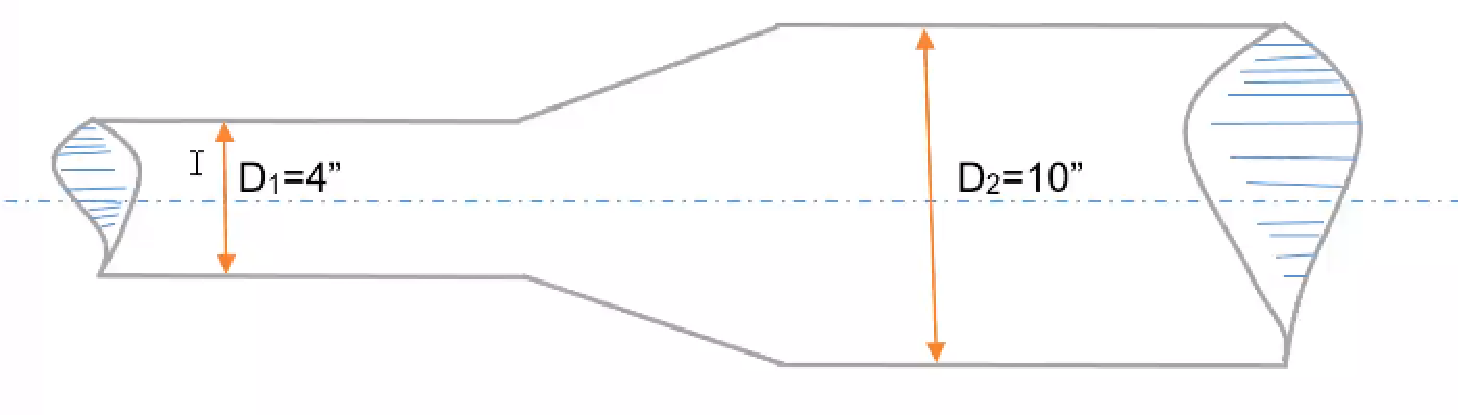
\includegraphics[width=0.5\textwidth]{hb53.pdf}
  \caption{Esquema del problemas}
  \label{hb53}
\end{figure}

\textit{ Sol. }

La viscosidad cinemática a $29^{\circ}C$ es $0.848\times 10^{-6}m^2/s$ aplicando la ecuación de continuidad en el tramo de $4^{\prime\prime}$ y en el de $10^{\prime\prime}$:
\begin{align*}
    &Q = A_1V_1 = A_2V_2\\
    &V_1 =\frac{Q}{A_1} =\frac{Q}{\frac{\pi D_1^2}{4}} =\frac{4\left( 0.0004\frac{m^3}{s} \right)}{\pi (0.1016m)^2} =0.04934\frac{m}{S}\\
    &V_2 =\frac{Q}{A_2} =\frac{Q}{\frac{\pi D_2^2}{4}} =\frac{4\left( 0.0004\frac{m^3}{s} \right)}{\pi (0.254m)^2} =0.007894\frac{m}{S}\\
    &Re_1 =\frac{V_1D_2}{v} =\frac{(\frac{0.04934m}{s})(0.1016m)}{0.848\times \frac{m^2}{s}} = 364.5\\
    &Re_1 = 911.25 > 4,000\implies \text{Flujo turbulento}\\
    &Re_2 = 2364.5\in (2000,4000)\implies \text{Flujo Transicional}\\
\end{align*}

\subsection{Número de Froude}

El número de Froude, interviene en la diferenciación de tipo de saltos hidráulicos y tipos de régimen en canales, en el diseño geométrico de disipadores de energía cinética, así como modelación hidráulica, entre otras cosas, su fórmula es: 

\begin{equation}
    Fr = \frac{v}{\sqrt{gD}}
\end{equation}
En la que $Fr$ es número de Froude (adimensional), $v$ es velocidad media $m/s$ y $g$ es la aceleración de la gravedad terrestre $(9.80665m/s^2)$ y $D=\frac{A}{T}=\frac{\text{Área hidráulica }m^2}{\text{Ancho de la S.L.A }m}$

\subsubsection{Clasificación de las corrientes líquidas}

Para clasificar las corrientes líquidas, se utilizan los siguientes criterios: 
\begin{enumerate}
    \item De acuerdo con el movimiento de sus partículas: \begin{enumerate}
        \item \textbf{Laminar} Se presenta en flujo medio poroso
        \item \textbf{Turbulento} Se presenta en tuberías, canales y ríos
    \end{enumerate}
    \item De acuerdo con la constancia de su gasto \begin{enumerate}
        \item \textbf{Continua} Cuando en todo su desarrollo el gasto es el mismo, en tuberías simples
        \item \textbf{Discontinua} CUando el gasto es diferente en su desarrollo, en tuberías ramificadas
    \end{enumerate}
    \item De acuerdo con la variación respecto al tiempo: \begin{enumerate}
        \item \textbf{Permanentes o establecidas} Cuando no varían las características de la sección respecto al tiempo y a las coordenadas del espacio $\frac{dy}{dt}=0$
        \item \textbf{Presión de flujo variable} Cuando las características de la sección no son variables respecto al tiempo y a las características del espacio $\frac{dy}{dt}\neq 0$ por ejemplo el llenado y vaciado de tuberías, en variación de gasto en canales y tuberías
        \end{enumerate}
    \item De acuerdo con su régimen \begin{enumerate}
        \item \textbf{Corrientes de régimen uniforme} Son aquellas que sus elementos técnicos se mantienen constantes en todo su desarrollo. por lo que el tirante, la velocidad, el gasto y la geometría de su sección normal, no cambian, esto es posible en canales artificiales, por ello reciben el nombre de canales prismáticos. $\frac{dy}{dx}=0$
        \item \textbf{Corrientes de régimen variado} Son aquellas constantes en su desarrollo $\frac{dy}{dx}\neq 0$\begin{enumerate}
            \item Variación en forma brusca (salto hidráulico)
            \item Gradual (remanso)
        \end{enumerate}
    \end{enumerate}
\end{enumerate}

\subsection{Tipos de energía hidráulica}
Los tipos de energía que se presentan en el movimiento de los líquidos son la energía cinética, la energía potencial y la energía de presión.
\begin{enumerate}
    \item La energía cinética de un cuerpo líquido o energía de movimiento, es la energía que posee el agua al adquirir velocidad.
    \begin{equation}
        E_c = \frac{1}{2}mv^2 = W = \frac{v^2}{2g}
    \end{equation}
    En una corriente líquida normalmente las energías se consideran por unidad de peso ($W=1$). Denominándose: Cargas, por lo tanto, en este
    caso la energía cinética se representa por la carga de velocidad $[L]$
    \begin{equation}
        h_v = \frac{v^2}{2g}
    \end{equation}
    \item La energía de presión es la que puede suministrar
    el líquido por la acción de contacto del mismo. 
    \begin{equation}
        Epr= W \frac{p}{\omega}
    \end{equation}
    En un líquido esta energía se representa por
    la carga de presión es $h_p=\frac{p}{\bar{\omega}}$
    \item Energía potencial Es la energía que suministra
    o adquiere un líquido al cambiar este de
    elevación con respecto a un nivel de referencia. por cuyo motivo se le llama también energía de posición.
    \begin{equation}
        E_{pot} = Wh
    \end{equation}
    En una corriente esta energía se representa por la carga de posición $(hz)$    
    \begin{figure}[h!]
    \centering
      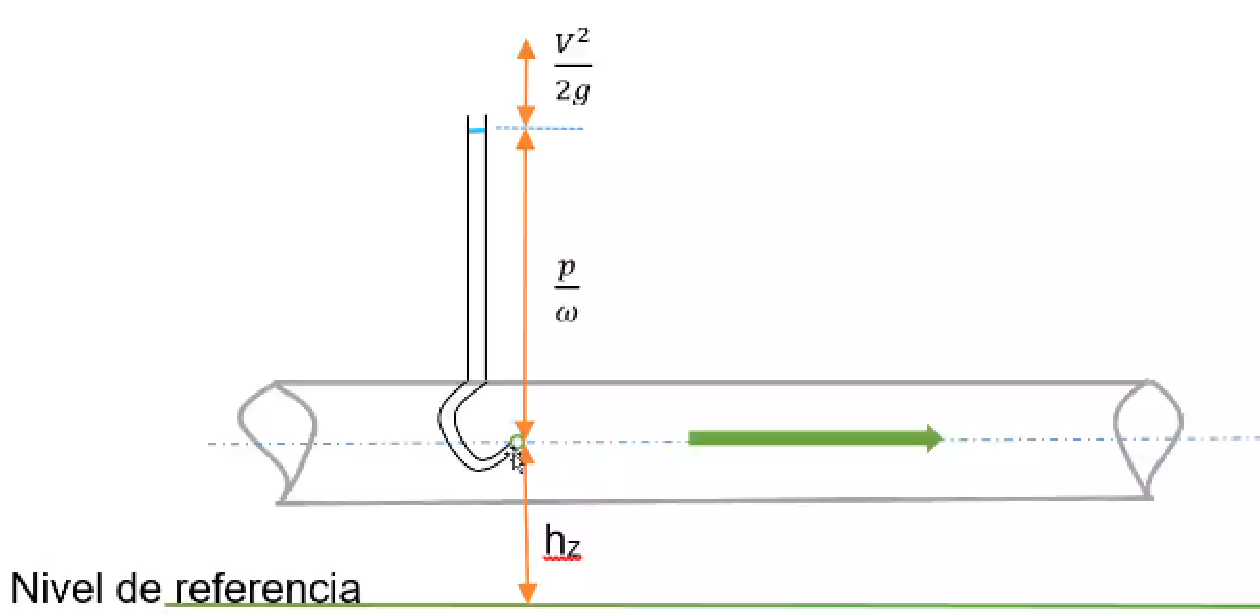
\includegraphics[width=0.5\textwidth]{hb54.pdf}
      \caption{Tubería con las cargas de presión}
      \label{hb54}
    \end{figure}
\end{enumerate}

\begin{theorem}[Teorema de Bernoulli (Ecuación de conservación de energía)]
    Esta ecuación tiene dos expresiones, una teórica para líquidos ideales y otra para práctica de líquidos reales.
    \textbf{Teórica:} En un líquido ideal sometido a la acción de la gravedad y en movimiento permanente (no dependiente del tiempo) en el camino que sigue la partícula, la suma de las cargas de posición, de presión y de velocidad, es constante.
    \begin{equation}
        z_1 + \frac{p_1}{\omega} + \frac{v^{2}_1}{2g} = z_2 + \frac{p_2}{\omega}+ \frac{p_2}{\omega} = z_2 +\frac{v^{2}_2}{2g} = C
    \end{equation}
    \textbf{Práctica:} En dos puntos de una corriente líquida entre las cuales el gasto es constante, la carga total del punto aguas arriba es igual a la carga total del otro más las pérdidas de carga entre ellos.
    \begin{equation}
        z_1 + \frac{p_1}{\omega} + \frac{v^{2}_1}{2g} = z_2 + \frac{p_2}{\omega}+ \frac{p_2}{\omega} +\sum_1^2 h_f
    \end{equation}
\end{theorem}
\begin{tikzpicture}
    \def\XSTART{0}
    \def\YSTART{3}
    \def\YDIAONE{2.5}
    \def\YDIATWO{2}
    \def\YCURVE{2}
    \def\XCURVE{2}
    \def\XEND{15}
    \def\XONESTART{2}
    \def\XONEDELTA{2}
    \def\DD{0.5}
  
    \def\YEND{\YSTART+\YCURVE+\YDIATWO}
    \def\XCURVESTART{\XEND/2-\XSTART/2-\XCURVE/2}
    \def\XCURVESTARTUP{\XEND/2-\XSTART/2-\XCURVE}
    \def\XCURVEEND{\XEND/2-\XSTART/2 + \XCURVE/2}
    \def\XONEEND{\XONESTART+\XONEDELTA}
    \def\XTWOSTART{\XCURVEEND+\XONESTART}
    \def\XTWODELTA{\XONEDELTA*\YDIAONE*\YDIAONE/\YDIATWO/\YDIATWO}
    \def\XTWOEND{\XTWOSTART+\XTWODELTA}
    \def\YTWOMIDDLE{\YSTART+\YCURVE+\YDIATWO/2}
    \def\YONEMIDDLE{\YSTART+\YDIAONE/2}
    \def\GROUND{\YSTART/4}
  
    \tikzset{
        partial ellipse/.style args={#1:#2:#3}{
            insert path={+ (#1:#3) arc (#1:#2:#3)}
        },
        dimen/.style={<->,>=latex,thin,
          every rectangle node/.style={fill=white,midway,font=\sffamily}},
    }
  
    \draw (\XSTART,\YSTART) -- (\XCURVESTART,\YSTART)
      to[out=0, in=180, looseness=0.75]
        (\XCURVEEND,{\YSTART+\YCURVE}) -- (\XEND,{\YSTART+\YCURVE});
    \draw (\XSTART,{\YSTART+\YDIAONE}) -- (\XCURVESTARTUP,{\YSTART+\YDIAONE})
      to[out=0, in=180, looseness=0.75] (\XCURVEEND,\YEND) -- (\XEND,\YEND);
  
    \draw [fill=gray] (\XONESTART,\YSTART) coordinate (BA)
      rectangle (\XONEEND,{\YSTART+\YDIAONE}) coordinate (BB);
    \draw [fill=lightgray](\XONESTART,\YONEMIDDLE) node [below] {$A_1$}
      ellipse ({\YDIAONE/6} and {\YDIAONE/2});
    \draw [fill=gray,dashed](\XONEEND,\YONEMIDDLE)
      ellipse ({\YDIAONE/6} and {\YDIAONE/2});
    \draw (\XONEEND,\YONEMIDDLE)
      [partial ellipse=-90:90:{\YDIAONE/6} and {\YDIAONE/2}];
  
    \draw [fill=gray] (\XTWOSTART,{\YSTART+\YCURVE}) coordinate (CA)
      rectangle (\XTWOEND,{\YSTART+\YCURVE+\YDIATWO}) coordinate (CB);
    \draw [fill=lightgray] (\XTWOSTART,\YTWOMIDDLE) node [below] {$A_2$}
      ellipse ({\YDIATWO/6} and {\YDIATWO/2});
    \draw [fill=gray,dashed](\XTWOEND,\YTWOMIDDLE)
      ellipse ({\YDIATWO/6} and {\YDIATWO/2});
    \draw (\XTWOEND,{\YSTART+\YCURVE+\YDIATWO/2})
      [partial ellipse=-90:90:{\YDIATWO/6} and {\YDIATWO/2}];
  
    \draw [fill=gray] (0,0) rectangle  (\XEND,\GROUND);
  
    \draw ($(BA)+(0,\YDIAONE)$) -- ++(0,\DD) coordinate (D1) -- +(0,5pt);
    \draw (BB) -- ++(0,\DD) coordinate (D2) -- +(0,5pt);
    \draw [dimen] (D1) -- (D2) node {$v_1dt$};
  
    \draw ($(BA)!0.5!(BB)$) -- ++(5pt,0) coordinate (E) -- +(5pt,0);
    \draw [dimen] let \p{E}=(E) in (\x{E},\GROUND) -- (E) node {$h_1$};
    \draw [style=->](\XSTART,\YONEMIDDLE) -- (\XONESTART,\YONEMIDDLE)
      node [midway,above] {$p_1$};
  
  
    \draw ($(CA)+(0,\YDIATWO)$) -- ++(0,\DD) coordinate (D1) -- +(0,5pt);
    \draw (CB) -- ++(0,\DD) coordinate (D2) -- +(0,5pt);
    \draw [dimen] (D1) -- (D2) node {$v_2dt$};
  
    \draw ($(CA)!0.5!(CB)$) -- ++(5pt,0) coordinate (D) -- +(5pt,0);
    \draw [dimen] let \p{D}=(D) in (\x{D},\GROUND) -- (D) node {$h_2$};
    \draw [style=->](\XCURVEEND,\YTWOMIDDLE) -- (\XTWOSTART,\YTWOMIDDLE)
      node [midway,above] {$p_2$};
\end{tikzpicture}
\begin{figure}[h!]
\centering
  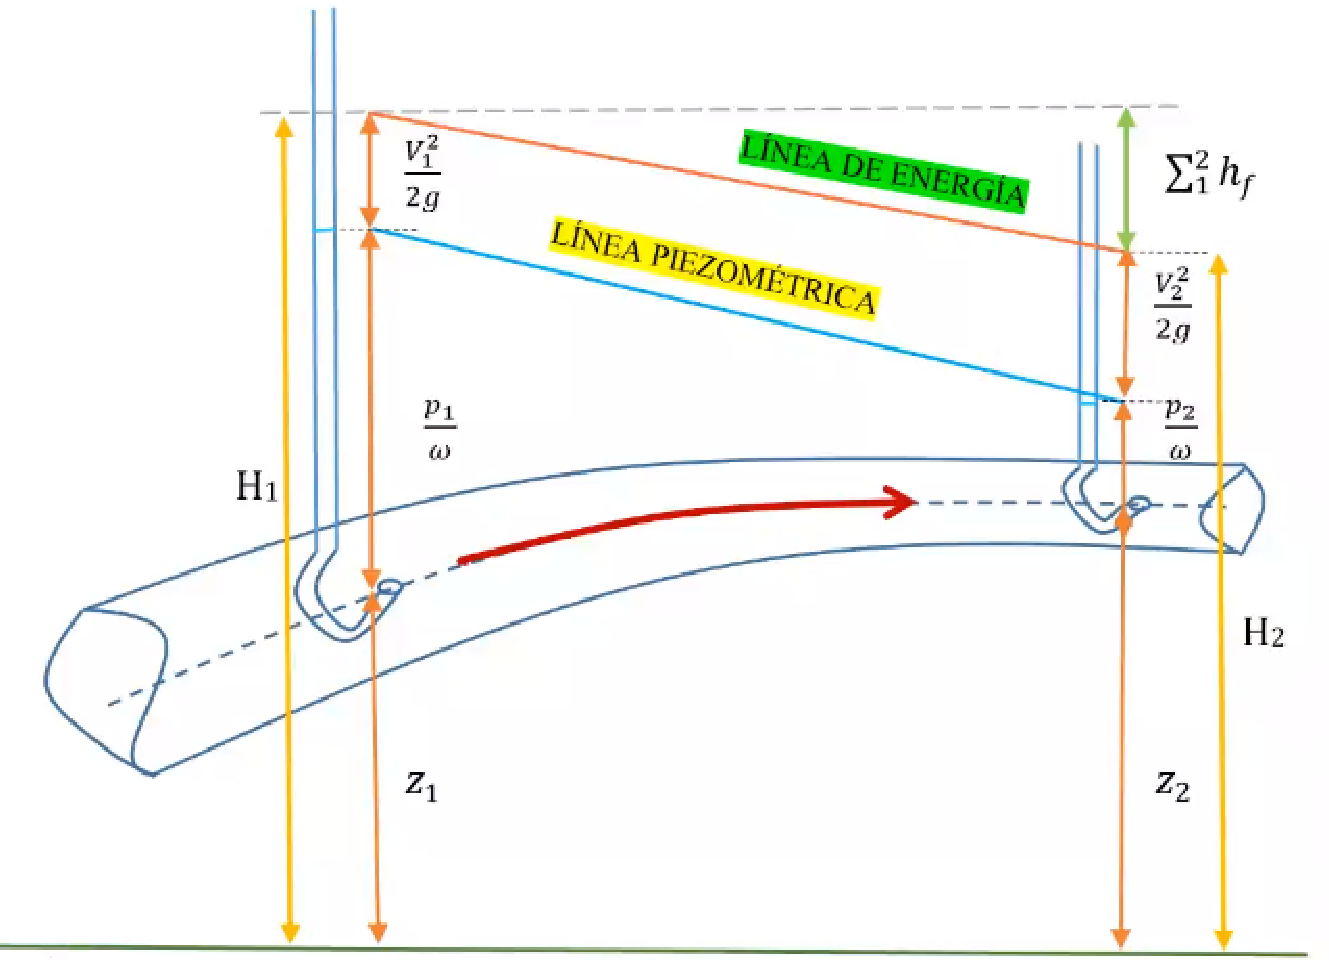
\includegraphics[width=0.5\textwidth]{hb55.pdf}
  \caption{Teorema de Bernoulli}
  \label{hb55}
\end{figure}

La diferencia de cargas totales entre dos puntos de una corriente continua, esto es la pérdida de carga es de dos tipos:

\begin{enumerate}
    \item \textbf{Por fricción} Las cuales es común ser evaluadas con la fórmula de Darcy- Weisbach.
    \begin{equation}
        h_f = f \frac{L\cdot v^2}{D\cdot 2g}
    \end{equation}
    \item \textbf{Localizadas} Las cuales es común ser evaluadas por 
    \begin{equation}
        h_x = k_x \frac{v^2}{2g}
    \end{equation}
\end{enumerate}

\subsubsection{Principio de Momentum (cantidad de movimiento)}

De la segunda ley de Newton: $F=ma$
\begin{align*}
    &F = m \frac{dv}{dt}\\
    &\int F\,dt =\int m\,dv\\
    &F\left( t_2 - t_1 \right) = \left( v_2 - v_1 \right)
\end{align*}
Donde $F_t$ es el impulso y $M(v_2-v_1)$ es la cantidad de movimiento. Se emplea en el cálculo de salto hidráulico:
\begin{align*}
    &F = \frac{\frac{W}{t}}{g}\left(v_2 - v_1\right)\\
    &\vec{F} = \frac{\frac{W}{t}}{g}v
\end{align*}
Expresión que permite calcular las presiones hidrodinámicas y por la tercera ley de Newton. A toda acción corresponde una reacción de la misma magnitud pero con dirección contraria.
\begin{equation}
    \vec{F} =\frac{\frac{W}{t}}{g}v =\overleftarrow{R} 
\end{equation}
La fuerza F empuja las partículas de agua a salir por el orificio, el recipiente de la figura, al abrir instantáneamente la válvula, recibe hacia la parte interna de pared una fuerza R, que lo hace girar un poco en dirección de las manecillas del reloj.

\begin{figure}[h!]
\centering
  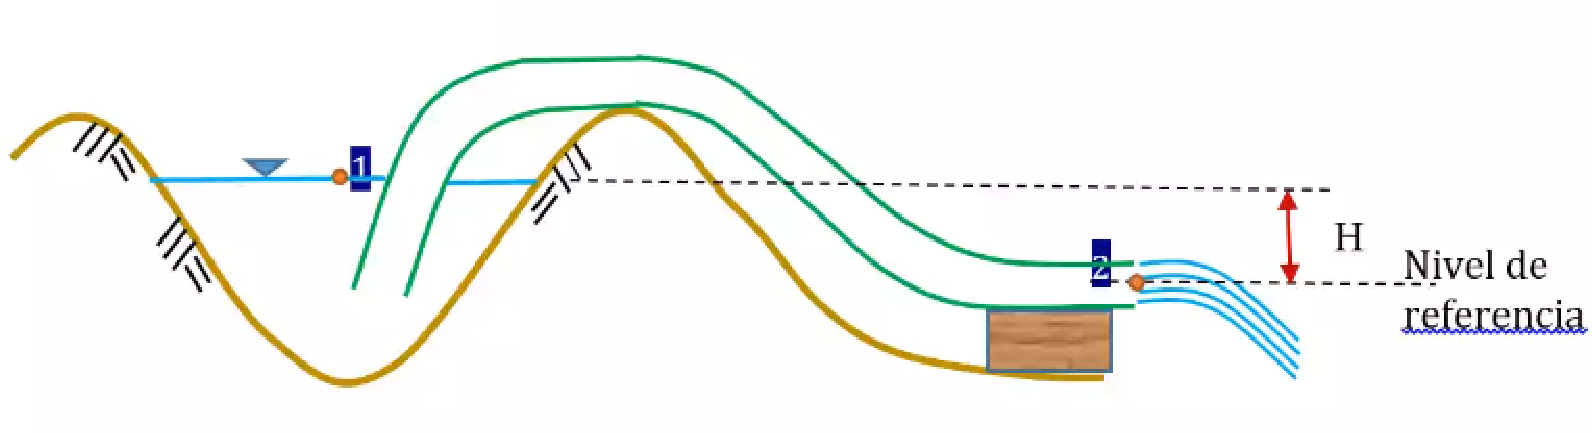
\includegraphics[width=0.5\textwidth]{hb56.pdf}
  \caption{Sifón}
  \label{hb56}
\end{figure}    

Aplicando el teorema de Bernoulli entre uno y dos (presiones relativas)
\begin{align*}
        &z_1 + \frac{p_1}{\omega} + \frac{V_1^2}{2g} = z_2 + \frac{p_2}{\omega} + \frac{v_2^2}{2g} +\sum_1^2 h_f\\
        &H = \frac{V_2^2}{2g} + \sum_1^2 h_f
\end{align*}
Si la sumatoria es igual a cero, el líquido ideal, la velocidad teórica con el líquido en el sifón será:
\begin{equation}
    V_{teorica} = \sqrt{2gH}
\end{equation}
De la cual despejando la velocidad, queda:
\begin{equation}
    V = \frac{1}{\sqrt{1 + k}}\sqrt{2gH}
\end{equation}

Si $C_v$ es coeficiente de velocidad obtenido experimentalmente, $C_v$ y $k$ quedan relacionados con la ecuación de Freeman (k>0 y $C_v$<1)
\begin{align*}
    &C_v = \frac{1}{\sqrt{1 + k}}&&j = \frac{1}{C_v^2} 1
\end{align*}
Quedando la velocidad como:
\begin{theorem}[Teorema de Torricelli]
    Para líquidos reales:
    \begin{equation}
        V_{real} = C_v \sqrt{2gH}
    \end{equation}
Al multiplicar esta velocidad por el área transversal de flujo, se obtiene el gasto, el cual quedaría como la fórmula general de un orificio, en la que para el caso del sifón, el coeficiente de descarga $C=C_v$
\begin{equation}
    Q = CA \sqrt{2gH}
\end{equation}
\end{theorem}
Las pérdidas de carga pueden ser expresadas en varias formas:
\begin{align}
    &\sum_1^2 h_f = k \frac{V_2^2}{2g}\\
    &\sum_1^2 h_f = H - \frac{v_2^2}{2g} =\left(1 - C_v^2\right)H\\
    &\sum_1^2 h_f = \frac{k}{1 + k}H   
\end{align}

\begin{problem}[Obtenga el gasto y las pérdidas de]
    en un sifón de $2 \frac{1}{2}^{\prime\prime}$ y 27 cm de carga. La $k=0.78$ y $N=30cm$. Determine la presión en $C$. ¿Qué lámina de riego aplican dos sifones durante una hora de operación a una melga de 1.2m de ancho y 154m de largo?
\end{problem}

\begin{figure}[h!]
\centering
  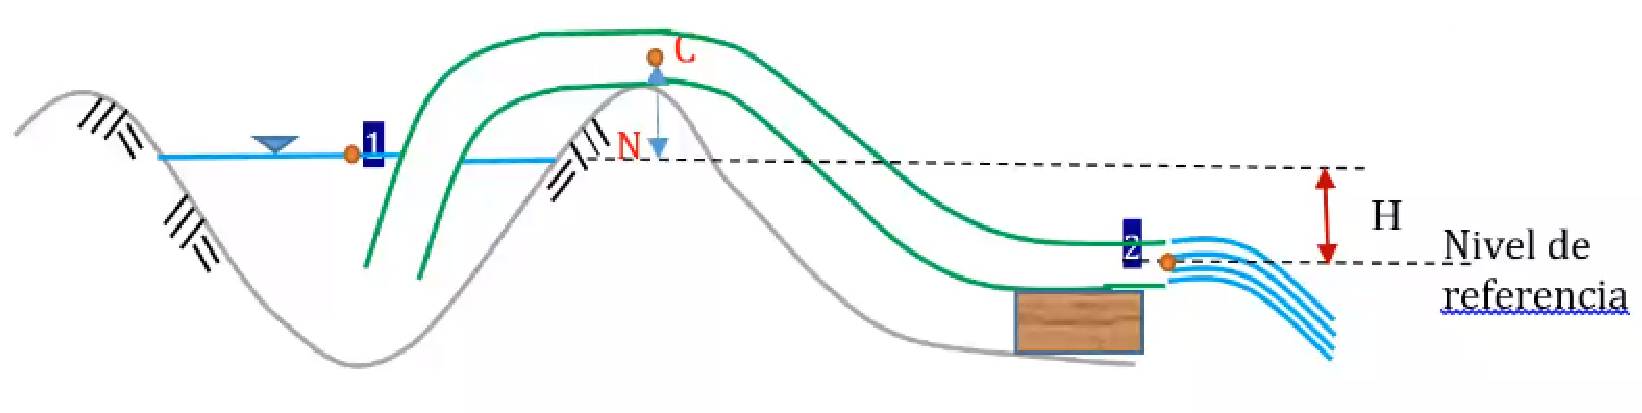
\includegraphics[width=0.5\textwidth]{hb57.pdf}
  \caption{Esquema del surco y los sifones}
  \label{hb57}
\end{figure}

\textit{ Sol. }

\begin{enumerate}
    \item La velocidad del agua en el sifón es:
    \begin{equation*}
        V_{real} = C_v \sqrt{2gH} = 0.7495 \sqrt{2g(0.27m)} = 1.725\frac{m}{s}
    \end{equation*}
    La ecuación de Freeman:
    \begin{equation*}
        C_v = \frac{1}{\sqrt{1 + k}} = \frac{1}{\sqrt{1 + 0.78}} =0.7495
    \end{equation*}
    El gasto que descarga el sifón es:
    \begin{equation*}
        Q = CA \sqrt{2gH} =0.7495 \frac{\pi(0.0635m)^2}{4}\sqrt{2g(0.27m)} = 5.46lps
    \end{equation*}
    \item Las pérdidas de carga:
    \begin{align*}
        &\sum_1^2 h_f = k \frac{V_2^2}{2g} = \frac{1.725^2}{2g} = 0.1183m\\
        &\sum_2^2 h_f = \left( 1 - C_v^{2} \right)H =(1 -0.7495^2)0.27 = 0.1183m\\
        &\sum_3^2 h_f = \frac{k}{1 + k}H = \frac{0.78}{1 +0.78}0.27 = 0.1183m
    \end{align*}
    \item Para obtener la presión en la parte alta del sifón (punto c) se aplicará el teorema de Bernoulli entre 1 y c, con el nivel de referencia pasando por el punto 1.
    \begin{align*}
        &z_c = \frac{p_{1}}{\omega} + \frac{v_{1}^2}{2g} = z_c + \frac{pc}{\omega} + \frac{V_c^2}{2g} +\sum_1^c hf\\
        &0 = N + \frac{p_c}{\omega} + \frac{V_c^2}{2g} +\sum_1^c h_f\\
        &\frac{p_c}{\omega} =- \left[N + \frac{V_c^2}{2g} + \sum_1^c h_f\right]
    \end{align*}
    Asumiendo la hipótesis de $\sum_1^c h_f= \frac{2}{5}\sum_1^2 h_f= \frac{2}{5}k\cdot \frac{v_c^2}{2g}$
\begin{align*}
        &\frac{p_c}{\omega} =-\left[N + \frac{V_c^2}{2g} + \frac{2}{5}k \cdot \frac{V_c^2}{2g}\right] =-\left[N +\left(1 + \frac{2}{5}k\right)\frac{V_c^2}{2g}\right]\\
        &\frac{p_c}{\omega} =- \left[0.3 +\left(1 + \frac{2}{5}(0.78)\right)_.725^\frac{2}{2g}\right] =-0.499m\\
        &p_c =-0.499m\cdot 1,000 \frac{kg}{m^3} =- 499 \frac{kg}{m^2}
    \end{align*}
    \item La lámina de riego aplicada por los dos sifones en una hora se obtiene dividiendo el volumen descargado entre el área de la melga:
    \begin{equation*}
        L_R = \frac{2Qt}{A_{melga}} = \frac{2\left( 0.00546 \frac{m^3}{s} \right)(60\cdot 60s)}{1.2\cdot 154m^2} =0.213m = 21.3cm
    \end{equation*}
\end{enumerate}
\begin{figure}[h!]
    \centering
      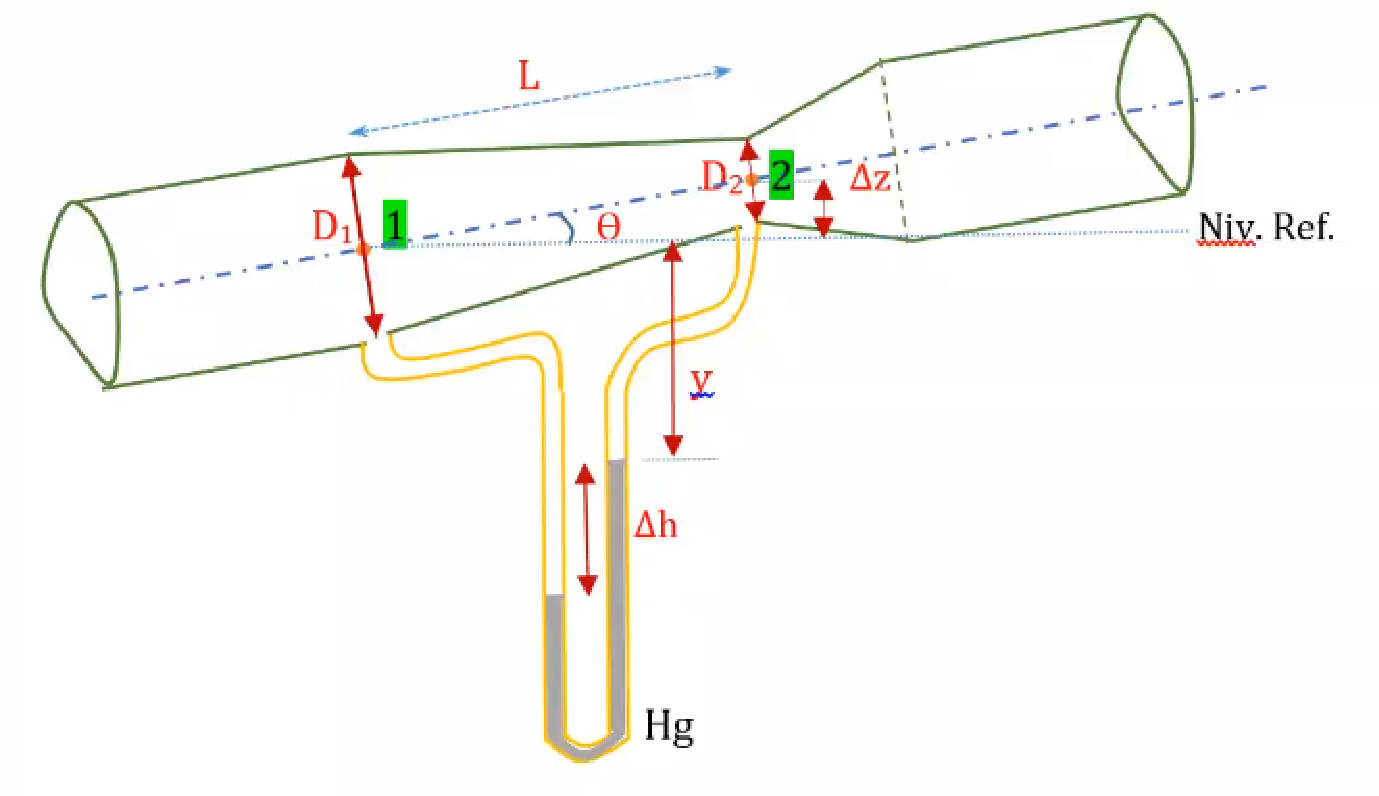
\includegraphics[width=0.5\textwidth]{hb58.pdf}
      \caption{Tubo de Venturi}
      \label{hb58}
    \end{figure}
    
    Aplicando el teorema de Bernoulli entre 1 y 2:
    \begin{align*}
        &z_1+ \frac{p_1}{\omega} + \frac{V_1^2}{2g} = z_2 + \frac{p_2}{\omega} + \frac{V^{2}_2}{2g} +\sum_1^2 h_f\\
        &\Delta Z + \frac{V_2^2}{g_2} + + k \frac{V_2^2}{2g} = \frac{p_1}{\omega} - \frac{p_2}{\omega} \\
        &(1 + k) \frac{V_2^2}{2g} - \frac{V_1^2}{2g} = \frac{p_1}{\omega} - \frac{p_2}{\omega} - \Delta Z
    \end{align*}
    La diferencia de presiones se obtiene con el manómetro diferencial aplicando el método americano:
    \begin{align*}
        &p_1 + y\omega +\Delta h\omega -\Delta h\omega_{Hg} - y\omega - Delta z\omega = p_2\\
        &\frac{p_1}{\omega} - \frac{2}{\omega} =\Delta g\left(\frac{\omega_{Hg} -\omega}{\omega}\right) +\Delta Z\\
        &(1 + k)\frac{V_2^2}{2g} - \frac{V_1^2}{2g}?\frac{p_1}{\omega} - \frac{p_2}{\omega} - Delta z =\Delta h\left(\frac{\omega_{Hg} -\omega}{\omega}\right) + Delta Z -\Delta z\\
        &(1 + k) \frac{V_2^2}{2g} - \frac{V_1^2}{2g} =\Delta h\left(\frac{\omega_{Hg} -\omega}{\omega}\right)
    \end{align*}
    
    Aplicando la ecuación de continuidad entre 1 y 2 tenemos:
    \begin{align*}
        &A_1V_1 = A_2V_2\\
        &\frac{\pi D_1^2}{4}V_1 = \frac{\pi D_2^2}{4}V_2\\
        &\frac{V_1^2}{2g} =\left(\frac{\frac{\pi D_2^2}{4}}{\frac{\pi D_1^2}{4}  }\right)\frac{V_2^2}{2g} =\left(\frac{D_2}{D_1}\right)^4\frac{V_2^2}{2g}\\
        &(1 + k)\frac{V_2^2}{2g} -\left(\frac{D_2}{D_1}\right)^{4}\frac{V_2^2}{2g} =\Delta h\left(\frac{\omega_{Hg} -\omega}{\omega}\right)\\
        &V_2 =\frac{1}{\sqrt{\left(1 + k -\left(\frac{D_2}{D_1}\right)^4\right)}} = \sqrt{2g\Delta h\left(\frac{\omega_{Hg} -\omega}{\omega}\right)}
    \end{align*}

    \begin{problem}[El gasto en el tubo de venturi]
        de $2\frac{1}{2}^{\prime\prime}$ en la tubería de $4^{\prime\prime}$ con un $k=0.35$ y un $\Delta h=14.2cm$ ¿Qué velocidad media tiene el agua en el estrechamiento y en la tubería? ¿Cuánto valen las pérdidas de carga?
    \end{problem}
    \textit{ Sol. }
    \begin{align*}
        &Q = \frac{\frac{\pi(0.0635m)^2}{4}}{\sqrt{1 +0.35 -\left(\frac{2.5}{4}\right)^4}}\cdot \sqrt{2g(0.142m)\cdot \left(\frac{13595 - 1,000}{1,000}\right)} = 0.01714 \frac{m^3}{s} = 17.14lps\\
        &V_2 = 5.413\frac{m}{s}\quad V_1 = 2.115 \frac{m}{s}\\
        &\sum_1^2 h_f = k \frac{v_2^2}{2g} =0.35 \frac{5.416^2}{2g} = 0.523m
    \end{align*}
    
\section{Flujo de agua en orificios}
    
    \begin{definition}[Orificio]
        Son perforaciones de forma geométrica y perímetro cerrado, hechas por debajo de la superficie libre del líquido, en las paredes de depósitos, tanques, canales o tuberías. Las aberturas hechas hasta la superficie libre del líquido
    constituyen los vertedores.
    \end{definition}

    \subsubsection{Clasificación de orificios}
    Los orificios se pueden clasificar en función de los siguientes criterios: 
    \begin{enumerate}
        \item Por su funcionamiento:
        \begin{figure}[h!]
        \centering
          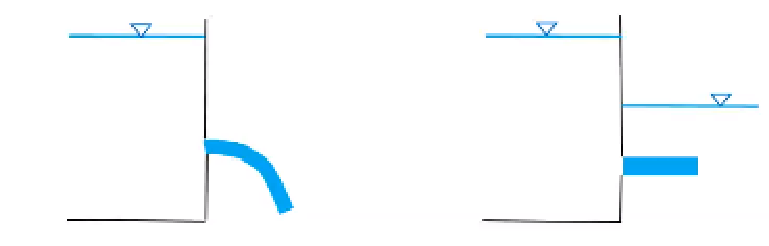
\includegraphics[width=0.5\textwidth]{hb59.pdf}
          \caption{Descargas Libres: cuando descargan al aire; descarga ahogada: cuando descargan en el interior de un líquido}
          \label{hb59}
        \end{figure}
        \item Por su geometría
        \begin{figure}[h!]
        \centering
          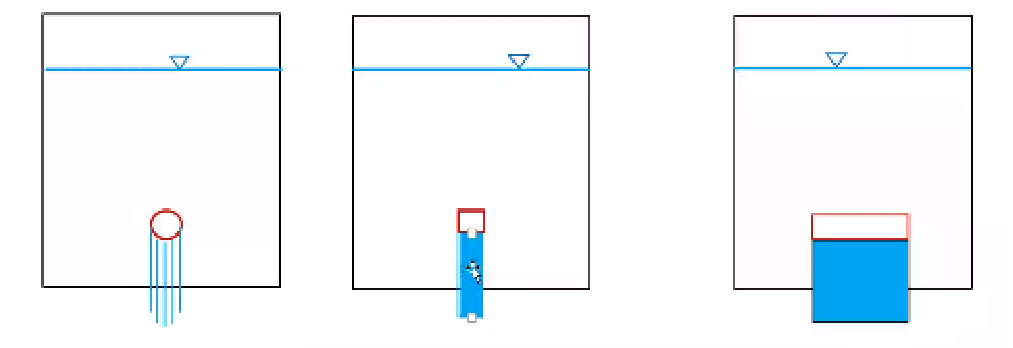
\includegraphics[width=0.5\textwidth]{hb60.pdf}
          \caption{Circulares, cuadrados y rectangulares}
          \label{hb60}
        \end{figure}
        \item Por el espesor de su pared
        \begin{figure}[h!]
        \centering
          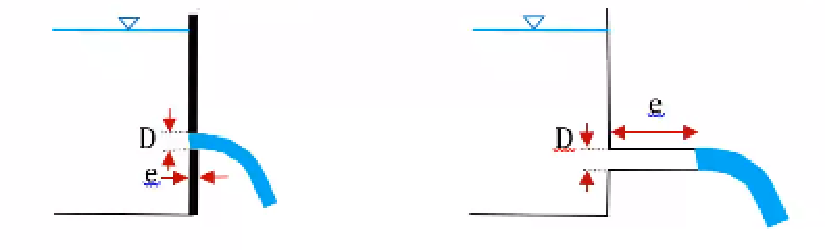
\includegraphics[width=0.5\textwidth]{hb61.pdf}
          \caption{Orificios de pared delgada ($e\leq 1.5D$) y orificios de pared gruesa $(e>1.5D)$}
          \label{hb61}
        \end{figure}
        \item Por sus dimensiones relativas
        \begin{figure}[h!]
        \centering
          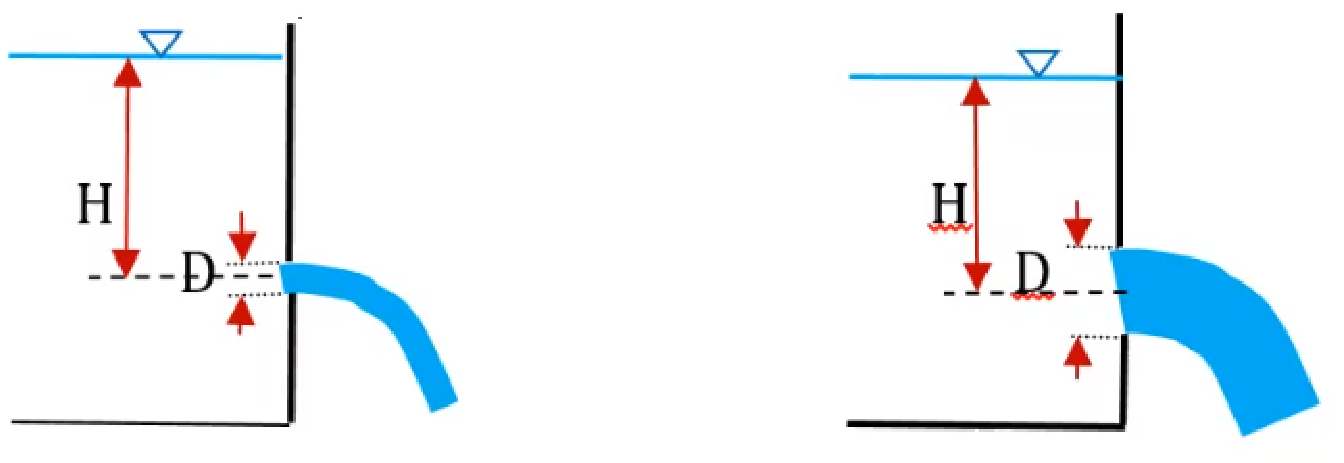
\includegraphics[width=0.5\textwidth]{hb62.pdf}
          \caption{Orificios pequeños $(D\leq H/3)$ y Orificios grandes $(D>H/3)$}
          \label{hb62}
        \end{figure}
    \end{enumerate}

    \subsubsection{Ecuación general del gasto en orificios pequeños}

    Considérese un orificio de pequeñas dimensiones de pared delgada biselada en la pared de un depósito (sin velocidad de llegada). Los filetes líquidos tocan el contorno del orificio convergiendo después de pasar por el mismo (debido a la inercia de las partículas), hasta una sección contraída, en la cual el chorro tiene un área sensiblemente menor que la del orificio. Aplicando el Teorema de Bernoulli entre la sección transversal al flujo entes del orificio y en la sección contraída, se obtiene:
    
    \begin{figure}[h!]
    \centering
      \includegraphics[width=0.5\textwidth]{hb63.pdf}
      \caption{Orificio}
      \label{hb63}
    \end{figure}
    
    \begin{equation*}
        h_{z1} + \frac{p_1}{\bar{\omega}} + \frac{v_1^2}{2g} = h_{z2} + \frac{p_2}{\bar{\omega}} + \frac{v_2^2}{2g} + \sum_1^2 h_f
    \end{equation*}
    
    considerando que la carga de velocidad en 1 es prácticamente nula y que su valor podría compensarse con la carga de presión en 2 que es $Dc/2$ aproximadamente, se
    tiene
    \begin{equation*}
        H = \frac{v_2^2}{2g} +\sum_1^2 h_f
    \end{equation*}
    de donde la velocidad en la sección contraída será:
    \begin{equation*}
        v_2 = \sqrt{2g\left(H -\sum_1^2 h_f\right)}
    \end{equation*}
    Observe que si se trata de un líquido ideal se tendría una expresión que es llamada ecuación de Torricelli.
    
    \begin{equation*}
        v_2 =\sqrt{2g\cdot H}
    \end{equation*}
    
    la cual proporciona velocidades mayores a la de un líquido real. La expresión práctica para un líquido real es:
    \begin{equation*}
        v_2 = C_v \sqrt{2g\cdot H}
    \end{equation*}
    
    en donde $C_v$ es coeficiente de velocidad cuyo valor es menor de 1.
    El gasto del orificio queda determinado por:
    \begin{equation*}
        Q = A_cv_2 = A_c v_2 = A_C C_v \sqrt{2gH}
    \end{equation*}
    Por definición, el coeficiente de contracción es $C_c= \frac{A_c}{A_0}\leq 1$, así:
    \begin{align*}
        &Q = C_c A_o C_v \sqrt{2gH}\\
        &Q = CA_o \sqrt{2gH}
    \end{align*}
    
    
    Para descarga ahogada es la misma fórmula y la carga H es la diferencia de niveles de agua, el del depósito que descarga y el nivel de ahogamiento.
    La pérdida de carga en un orificio (ho) se determina a partir del Teorema de Bernoulli. 
    \begin{equation*}
        H_0 = H - \frac{v_2^2}{2g}
    \end{equation*}
    pero como $H= \frac{2}{C_v^2}\cdot \frac{v_2^2}{2g}$ de la ecuación de la velocidad de un líquido real:
    \begin{equation*}
        h_0 = \frac{1}{C_v^2}\cdot \frac{v_2^2}{2g} - \frac{v_2^2}{2g} = \left(\frac{1}{C_v^2} - 1 \right) \frac{v_2^2}{2g} = h_0\cdot \frac{v_2^2}{2g}
    \end{equation*}
    donde $k_0= \frac{1}{C_v^2}-1$ es la expresión conocida como la ecuación de Freeman.
    
    Para entrada con aristas vivas (a escuadra) y alejado de planos y piso (3D cuando es circular o tercera dimensión menor cuando es rectangular) $C$ vale 0.61 (y $C_c=0.62$, entonces $Cv=\frac{C}{C_c}=0.984$) y para una entrada hidrodinámica (abocinada o tubos cortos) puede valer cerca de 1.
    
    Para un tubo corto que tiene una longitud de 2.5 a 3D, el valor de $C_v$ es de aproximadamente 0.82 y $C_c$ es de 1. ($C=0.82$)
    
    \begin{problem}[El tanque recibe un gasto de 43 LPS.]
        ¿Cuál es la carga en el tanque y el gasto en los orificios? Resolver en flujo establecido.
    \end{problem}
    \begin{figure}[h!]
    \centering
      \includegraphics[width=0.5\textwidth]{hb64.pdf}
      \caption{Esquema del problema}
      \label{hb64}
    \end{figure}
    
    \textit{ Sol. }
    
    Planteamos los nombres de las incógnitas
    
    \begin{figure}[h!]
    \centering
      \includegraphics[width=0.5\textwidth]{hb65.pdf}
      \caption{incógnitas definidas}
      \label{65}
    \end{figure}
    $D=0.1016m$ $H=0.1905$, $Q=0.94(0.0081073)(1.93329)$=
    Ecuación del sistema: $Q=Q_1+Q_2$, así:
    \begin{align*}
        &Q = C_1A_1 \sqrt{2gH} + C_2A_2 \sqrt{2g(H - 0.127)}\\
        &a_1 = C_1A_1 \sqrt{2g} =0.94 \left(\frac{\pi 0.1016^2}{4}\right) \sqrt{19.62} = 0.033756364\\
        &a_2 = C_2A_2 \sqrt{2g} =0.82 \left(\frac{\pi 0.0762^2}{4}\right) \sqrt{19.62} = 0.01656396\\
        &Q = a_1 \sqrt{H} + a_2 \sqrt{H - 0.127}
    \end{align*}
    Esta ecuación se resuelve por iteraciones, la solución es: $H=0.773m$ Así el gasto en cada orificio es $Q_1=0.033756364 \sqrt{0.773}=0.0296787 m^3/s$ y $Q_2=0.01656396 \sqrt{0.773-0.127}=0.00984 m^3/s$
    

    \begin{example}
        Determine el gasto en los orificios y las cargas en los tanques, si al tanque del centro le llegan 12 LPS.
    \end{example}
    
    \begin{figure}[h!]
    \centering
      \includegraphics[width=0.5\textwidth]{hb66.pdf}
      \caption{Esquema del problema}
      \label{hb66}
    \end{figure}
    
    \textit{ Sol. }
    
    Lo primero será etiquetar o nombrar los gastos y las cargas y plantear las ecuaciones del sistema.
    
    \begin{figure}[h!]
    \centering
      \includegraphics[width=0.5\textwidth]{hb67.pdf}
      \caption{Incógnitas definidas}	
      \label{hb67}
    \end{figure}
    
    Ecuaciones del sistema:
    \begin{equation*}
        \begin{cases}
            &Q = Q_1 + Q_3\\
            &Q_1 =Q_2\\
            &Q_3 = Q_4 
        \end{cases}
    \end{equation*}
    
    Cálculo de áreas constantes:
    \begin{align*}
        &A_{2^{\prime\prime}}=\frac{\pi D^2_1}{4} = \frac{\pi (0.0508m)^2}{4} = 0.0020268m^2\\
        &A_{2^{\prime\prime}}=\frac{\pi D^2_2}{4} = \frac{\pi (0.0635m)^2}{4} = 0.00316693m^2\\
    \end{align*}
    \begin{align*}
        &a_1 = C_1A_1 \sqrt{2g} = 0.82\cdot 0.0020268\cdot \sqrt{19.62} =  7.36176 \times 10^{-3}\\
        &a_2 = C_2A_2 \sqrt{2g} = 0.61\cdot 0.00316693\cdot \sqrt{19.62} = 8.556924 \times 10^{-3}\\
        &a_3 = C_3A_3 \sqrt{2g} = 0.82\cdot 0.00316693\cdot \sqrt{19.62} = 11.50275 \times 10^{-3}\\
        &a_4 = C_4A_4 \sqrt{2g} = 0.61\cdot 0.0020268\cdot \sqrt{19.62} =  5.47643 \times 10^{-3}\\
    \end{align*}
    Desarrollando las ecuaciones del sistema:
    \begin{align*}
        &Q = C_1A_1 \sqrt{2g}\left(H_2 - H_1\right)^{\frac{1}{2}}C_3A_3 \sqrt{2g}\left(H_4 - H_3\right)^{\frac{1}{2}}\\
        &Q = a_1\left(H_2 - H_1\right)^{\frac{1}{2}} + a_3\left(H_2 - H_3\right)^{\frac{1}{2}}\\
        &a_1\left(H_2 - H_1\right)^{\frac{1}{2}} = a_2 H_1^{\frac{1}{2}}\\
        &a_3\left(H_2 - H_3\right)^{\frac{1}{2}} = a_4 H_3^{\frac{1}{2}}
    \end{align*}
    
    Despejando $H_1$ de la ecuación tres:
    \begin{align*}
        &\left(a_1\left(H_2 - H_1\right)^{\frac{1}{2}}\right)^2 =\left(a_2H_1^{\frac{1}{2}}\right)^2\\
        &a_1^2\left(H_2 - H_1\right) = a_2^2H_1\\
        &H_1 =\left(\frac{a_1^2}{a_1^2 + a_2^2}\right)H_2 =b_1H_2\\
        &\therefore H_1 = b_1H_3
    \end{align*}
    \begin{equation*}
        b_1 = \frac{a_1^2}{a_1^2 + a_2^2} = \frac{0.00736176^2}{0.00736176^2 +0.008556924^2} =0.42534152
    \end{equation*}
    Despejando $H_3$ de la cuarta ecuación:
    \begin{align*}
        &\left(a_3(H_2 - H_3)^{\frac{1}{2}}\right)^{2} = \left(a_4\right)^2H_3\\
        &a_3^2(H_2 - H_3) = a_4^2H_3\\
        &H_3 = \left(\frac{a_3^2}{a_3^2 + a_4^2}\right)H_2 = b_2H_2\\
        &\therefore H_3 = b_2H_2
    \end{align*}
    \begin{equation*}
        b_2 = \frac{a_3^2}{a_3^2 + a_4^2} = \frac{0.001150275^2}{0.001150275^2 + 0.005475643^2} = 0.815216
    \end{equation*}
    
    Sustituyendo la ecuación cuatro y la ecuación cinco, en la ecuación 2:
    \begin{equation*}
        Q = 1\left(H_2 - b_1 H_2\right)^{\frac{1}{2}} + a_3\left(H_2 - b_2H_3\right)^{\frac{1}{2}}
    \end{equation*}
    Desarrollando y factorizando $H_2$:
    \begin{align*}
        &Q = a_1\left(1 - b_1\right)^{\frac{1}{2}}H_2^{\frac{1}{2}} + a_3\left(1 - b_2\right)^{\frac{1}{2}}H_2^{\frac{1}{2}} =\left(a_1\left(1 - b\right)^{\frac{1}{2}} + a_3\left(1 - b_2\right)^{\frac{1}{2}}\right)H_2^{\frac{1}{2}}\\
        &H_2 =\left(\frac{Q}{\left(a_1\left(1 - b_1\right)^{\frac{1}{2}} a_3\left(1 - b_2\right)^{\frac{1}{2}}\right)}\right)^2\\
        &H_2 =\left(\frac{0.012}{\left(0.00736176\left(1 - 0.42534152\right)^{\frac{1}{2}} + 0.01150275\left(1 - 0.815216\right)^{\frac{1}{2}}\right)}\right)^2\\
        &H_2 =0.29985m
    \end{align*}
    Sustituyendo $H_2$ en la tercera ecuación: $H_1=0.42534152(1.29985)=0.55288m$
    Sustituyendo $H_3$ en la cuarta ecuación: $H_3=0.815216(1.29985)=1.05969m$
    Los gastos en los orificios serán:
    \begin{align*}
        &Q_1 = a_1 \sqrt{H_2 - H_1} =0.00736176 \sqrt{1.29985 -0.55288} =0.006362578 \frac{m^3}{s}\\ 
        &Q_3 = a_3 \sqrt{H_2 - H_3} =0.001150275 \sqrt{1.29985 -1.05969} =0.0005637 \frac{m^3}{s}\\
        &Q_2 = a_2 \sqrt{H_1} = 0.008556924 \sqrt{0.55288} = 0.00636258 \frac{m^3}{s}\\
        &Q_4 = a_4 \sqrt{H_3} = 0.005475643 \sqrt{1.05969} = 0.005637 \frac{m^3}{s}\\
        &Q_1 + Q_3 = 0.01199958 \frac{m^3}{s}
    \end{align*}
    
    \begin{problem}[¿Qué diámetro debe tener el orificio cuatro para que $Q_2=Q_4$?]
        El gasto que le llega al tanque del centro 12+0.2n
    \end{problem}

    Ecuaciones del sistema:
    \begin{equation*}
        \begin{cases}
            &Q = Q_1 + Q_3\\
            &Q_1 =Q_2\\
            &Q_3 = Q_4 
        \end{cases}
    \end{equation*}
    De éste sistema, podemos desarrollar la siguiente equivalencia:
    \begin{align*}
        &Q = C_1 A_1 \sqrt{2g\left(H_2 - H_1\right)} + C_3A_3 \sqrt{2g\left(H_2 - H_3\right)}\\
        &C_1A_1 \sqrt{2g\left(H_2 - H_1\right)} = C_2A_2 \sqrt{2gH_1}\\
        &C_3A_3 \sqrt{2g\left(H_2 - H_3\right)} = C_4A_4 \sqrt{2gH_3}\\ 
        &C_2A_2 \sqrt{2gH_1} = C_4A_4 \sqrt{2gH_3}
    \end{align*}
    
    Cálculo de áreas constantes:
    \begin{align*}
        &A_{2^{\prime\prime}}=\frac{\pi D^2_1}{4} = \frac{\pi (0.0508m)^2}{4} = 0.0020268m^2\\
        &A_{2^{\prime\prime}}=\frac{\pi D^2_2}{4} = \frac{\pi (0.0635m)^2}{4} = 0.00316693m^2\\
    \end{align*}
\begin{align*}
        &a_1 = C_1A_1 \sqrt{2g} = 0.82\cdot 0.0020268\cdot \sqrt{19.62} =  7.36176 \times 10^{-3}\\
        &a_2 = C_2A_2 \sqrt{2g} = 0.61\cdot 0.00316693\cdot \sqrt{19.62} = 8.556924 \times 10^{-3}\\
        &a_3 = C_3A_3 \sqrt{2g} = 0.82\cdot 0.00316693\cdot \sqrt{19.62} = 11.50275 \times 10^{-3}\\
        &a_4 = C_4A_4 \sqrt{2g} = 0.61\cdot \pi \frac{D^2}{4} \cdot \sqrt{19.62} =  2.122116479 D^2\implies a_4 = bD^2\\
    \end{align*}
    Se plantean cuatro ecuaciones fundamentales a simplificar y dejar con las mismas incógnitas:
    \begin{align*}
        &Q = a_1 \sqrt{H_2 - H_1} + a_3 \sqrt{H_2 - H_3}\\
        &a_1 \sqrt{H_2 - H_1} = a_2 \sqrt{H_1}\\
        &a_3 \sqrt{H_2 - H_3} = a_4 \sqrt{H_3}\\
        &a_2 \sqrt{H_1} = a_4 \sqrt{H_3}
    \end{align*}
    
    Desarrollando el segundo punto:
    \begin{align*}
        &a_2^2H_1 = a_1^2\left(H_2 - H_1\right)\\
        &a_2^2H_2 = a_1^2H_2 a_1^2H_1\\
        &a_2^2H_1 + 1^2H_1 = a_1^2H_2\\
        &H_2\left(a_2^2 + a_1^2\right)\\
        &H_1 =\left(\frac{a_1^2}{a_2^2 a_1^2}\right)H_2\\
        &H_1 = d_1 H_2
    \end{align*}
    De donde se calcula $d_1$:
    \begin{equation*}
        d_1 =\frac{\left(7.361743132 \times 10^{ - 3}\right)^2}{\left(8.556904174\times 10^{ - 3}\right)^2 + \left(7.361743132 \times 10^{ - 3} \right)} = 0.4253415334
    \end{equation*}
    
    Despejando el tercer punto:
    \begin{align*}
        &a_3^2\left(H_2 - H_3\right)b^2D^4H_3\\ 
        &D^4 = \frac{a_3^2\left(H_2 - H_3\right)}{b^2H_3}
    \end{align*}
    Sustituyendo en la cuarta ecuación:
    \begin{align*}
        &a_2^21 = b^3D^4H_3\\
        &D^4 = \frac{a_2^2H_1}{b^2H_3}	
    \end{align*}
    Igualando los productos de ésta tercera y cuarta ecuación, podemos igualar:
    \begin{align*}
        &\frac{a_3^2\left(H_2 - H_3\right)}{b^2H_3} = \frac{a_2^2H_1}{b^2H_3}\\
        &a_3^2\left(H_2 - H_3\right) = a_2^2\left(H_1\right)\\
        &a_3^2H_2 - a_3^2H_3 = a_2^2H_1\\
        &H_3 = \frac{a_3^2H_2 - a_2^2H_1}{a_3^2}\\
        &H_3 = H_2  - \frac{a_2^2}{a_3^2}H_1\\
        &H_3 = H_2 - d_2H_1
    \end{align*}
    De ésta última ecuación, se deduce la quinta igualdad:
    \begin{equation*}
        H_3 = H_2 - d_2H_1
    \end{equation*}
    Finalmente se calcula $d_2$ como sigue:
    \begin{equation*}
        d_2  \frac{a_2^2}{a_3^2} = \frac{\left(8.556904174 \times 10^{ - 3}\right)^2}{\left(11.50272364 \times 10^{ - 3}\right)^2} =0.5533908391
    \end{equation*}
    Sustituyendo la segunda ecuación en ésta quinta nueva, obtenemos:
    \begin{equation*}
        H_3 = H_2 - 2H_1\implies H_3 = H_2 - d_2d_1 H_2
    \end{equation*}
    Ahora, de la segunda expresión derivada, se sustituye en ésta última:
    \begin{align*}
        &Q = a_1 \sqrt{H_2 - H_1} + a_3 \sqrt{H_2 - H_3}\\
        &Q = a_1 \sqrt{H_2 - d_1H_1} + a_3 \sqrt{H_2 - \left(H_2 - d_2d_1 H_2\right)} \\
        &Q = H_2\left[a_1\left(1 - 1\right)^{\frac{1}{2}} +a_3\left(d_2d_1\right)^{\frac{1}{2}} \right]\\
        &\therefore H_2 = \left[\frac{Q}{a_1\left(1 - 1\right)^{\frac{1}{2}} + a_3\left(d_1d_2\right)^{\frac{1}{2}}} \right]\\
        &H_2 =\left(\frac{0.01241}{5.580660008 \times 10^{ - 3} + 5.580660008 \times 10^{ - 3}}\right)^2\\
        &H_2 = \left(\frac{0.01241}{11.16132002 \times 10^{ - 3}}\right)^2 = 1.236237471m
    \end{align*}
    Sustituyendo $H_2$ en la segunda ecuación derivada obtenemos:
    \begin{equation*}
        H_1 = H_2 = (0.4253415334m)\cdot (1.236237471m) = 0.525823142 m^2
    \end{equation*}
    Sustituyendo $H_2$ en la quinta ecuación:
    \begin{equation*}
        H_3 = H_2 -d2H_1 = 1.236237471 - (0.5533908391)(0.525823142) = 0.94525176123m
    \end{equation*}
    Para determinar el valor $D$ en la cuarta ecuación que se simplificó:
    \begin{align*}
        &D^4 = \frac{a_2^2 H_1}{b^2H_3} = \frac{\left(8.556904174 \times 10^{ - 3}\right)^2(0.525823142)}{\left(2.122116479\right)^2(0.94525176123)}\\ 
        &D^4 = 9.044552875 \times 10^{ - 6} = 0.054839915m = 2.1590 pulg
    \end{align*}
    Comprobamos si los coeficientes son correctos:
    \begin{align*}
        &Q_1 = a_1 \sqrt{H_2 - H_1} = \left(7.361743132 \times 10^{ - 3}\right) \sqrt{1.236237471 - 0.525823142} = 0.006205 \frac{m^3}{s}\\
        &Q_2 = a_2 \sqrt{H_1} = \left(8.556904174 \times 10^{ - 3}\right) \sqrt{0.525823142} = 0.006205 \frac{m^3}{s}\\
        &Q_3 = a_3 \sqrt{H_2 - H_3} = \left(11.50274889 \times 10^{ - 3}\right) \sqrt{1.236237471 - 0.94525176123} = 0.006205 \frac{m^3}{s}\\
        &Q_4 = bD^2 \sqrt{H_3} = (2.122116479)(0.054839915)^2 \sqrt{0.94525176123} = 0.006205 \frac{m^3}{s}\\ 
        &\therefore Q = Q_1 + Q_3 = 0.006205 + 0.006205 = 0.01241 \frac{m^3}{s} = 12.41 lps
    \end{align*}
    Y por lo tanto también se cumple:
    \begin{align*}
        &Q_1 = Q_2 \implies 0.006205 = 0.006205\\
        &Q_3 = Q_4 \implies 0.006205 = 0.006205\\
        &Q_2 = Q_4 \implies 0.006205 = 0.006205 \quad \blacksquare 
    \end{align*}


\subsubsection{Flujo de carga variable a través de un orificio (Régimen transitorio, vaciado de depósitos)}

Se considera un depósito (De forma cualquiera) que se vacía a través de orificio localizado en el fondo.

\begin{figure}[h!]
\centering
  \includegraphics[width=0.5\textwidth]{hb68.pdf}
  \caption{Depósito con orificio}
  \label{hb68}
\end{figure}

Se supone que el depósito tiene una superficie horizontal $A(y)$ muy grande en comparación con el área del orificio ($A_0$), esto equivale a que la velocidad de descenso del nivel de la superficie libre del agua es de una magnitud prácticamente despreciable.

El gasto en cualquier instante $t$, es

\begin{equation}
    Q = CA_0 \sqrt{2gy}
\end{equation}
Un elemento diferencial de volumen $dv=A(y)\,dy$, se vacía en un $dt$ y como a mayor $t$, el volumen decrece, la ecuación diferencial queda:
\begin{align*}
    &Q =- \frac{dV}{dt}\\
    &dt =- \frac{A(y)\,dy}{CA_0 \sqrt{2gy}}
\end{align*}
Así el tiempo que transcurre para que el nivel de la superficie libre del agua pase de $h_1$ a $h_2$ es:
\begin{equation}
    t = \frac{1}{CA_0 \sqrt{2g}}\int A\frac{y}{\sqrt{y}}\,dy 
\end{equation}
Para diferentes formas del depósito, se requiere obtener la función $A(y)$ y se integra para obtener el tiempo.

Para el caso particular de paredes verticales del depósito $A$ no es función de $Y$ ya que es constante, y la solución queda:
\begin{equation}
    t = \frac{A}{CA_0 \sqrt{2g}}\int_{h2}^{h1}y^{\frac{1}{2}}\,dy = \frac{A}{CA_0 \sqrt{2g}}\left[\frac{y^{\frac{1}{2}}}{\frac{1}{2}}\right]_{h2}^{h1} = \frac{2A}{CA_0 \sqrt{2g}}\left(h_1^{\frac{1}{2}} - h_2^{\frac{1}{2}}\right)
\end{equation}
Si $h:2$ es cualquier carga $h$ en el depósito $h<h_1$, la función de vaciado $t(h)$ será:
\begin{equation*}
    t(h) = \frac{2A}{CA_0 \sqrt{2g}}\left(h_1^{\frac{1}{2}} - h^{\frac{1}{2}}\right)
\end{equation*}
Ahora si el vaciado es completo del depósito $h=0$, el tiempo de vaciado quedará:
\begin{equation*}
    t = \frac{2Ah^{\frac{1}{2}}_1}{CA_0 \sqrt{2g}}
\end{equation*}
Simplificando la expresión:
\begin{equation*}
    t = \frac{2Ah^{\frac{1}{2}_1}}{{cA_0 \sqrt{2g}}}\left(\frac{h^{\frac{1}{2}}_1}{h_1^{\frac{1}{2}}}\right) = \frac{2V_{dep}}{Q_{inicial}} = \frac{V_{dep}}{\frac{Q_i + Q_f}{2}} = \frac{V_{dep}}{Q_{med}}
\end{equation*}

\begin{example}
    Obtener el volumen descargado por el orificio, cuando el nivel de agua desciende 5 m en el depósito de la figura \ref{hb69}, y el tiempo en el cual, descarga dicho volumen.
\end{example}
\begin{figure}[h!]
\centering
  \includegraphics[width=0.5\textwidth]{hb69.pdf}
  \caption{Tolba}
  \label{hb69}
\end{figure}

\textit{ Sol. }

\begin{figure}[h!]
\centering
  \includegraphics[width=0.5\textwidth]{hb70.pdf}
  \caption{Esquema de la solución}
  \label{hb70}
\end{figure}

\begin{enumerate}
    \item El volumen descargado por el orificio es cuando $h$ desciende de 5.4m a 3m en la parte del depósito con paredes verticales $V_1$ y el volumen $V_2$ cuando la carga desciende de $3m$ a $0.4m$ en la parte piramidal del depósito.
    \begin{align*}
        &V_1 = m(4m)(2.4m) =192m^3\\
        &V_2 =\int_{0.4}^{3} A(h)\,dh = \int_{0.4}^{3}X(h)Y(h)\,dh
    \end{align*}
    $X(h)$ y $Y(h)$ son lineales y se obtienen en el sistema MKS, $X(h)$ pasa por los puntos $P_1:X(0)=0.3$ y $P_2:X(3)=4$. Así, $X(h)= \frac{3.7}{3}h+0.3$
    $Y(h)$ pasa por los puntos $P_1:Y(0)=0.3$ y $P_2:Y(3)=2$. Así $X(h)= \frac{1.7}{3}h+0.3$
    \begin{equation*}
        V_2 = \int_{0.4}^{3}\left(\frac{3.7}{3}h 0.3\right)\left(\frac{1.7}{3}h +0.3\right)\,dh = \int_{0.4}^{3}\left(\frac{629}{900}h^2 + \frac{4}{100}h + \frac{9}{100}\right)\,dh = 8.89589m^3
    \end{equation*}
    El volumen descargado es $19.2+8.89589=28.0959m^3$    
    \item El tiempo en el que desciende la carga de 5.4m a 3m será ($t_1$):
    \begin{align*}
        &t_1 = \frac{A}{CA_0 \sqrt{2g}}\int_3^{5.4}h^{ -\frac{1}{2}}\,dh = \frac{A}{CA_0 \sqrt{2g}}\left[\frac{h^{\frac{1}{2}}}{\frac{1}{2}} \right]_3^{5.4} = 768.182\left(5.4^{\frac{1}{2}} - 3^{\frac{1}{2}}\right) =454.56s = 7\min \, 34.56s\\
        &\frac{2A}{CA_0 \sqrt{2g}} =\frac{2\cdot 8}{0.58 \frac{\pi 0.1016^2}{4} \sqrt{2g}} = 68.182 
    \end{align*}
    En la parte piramidal, el tiempo en el que la carga desciende de 3m a 0.4m será $t_2$
    \begin{align*}
        &t_2 = \frac{1}{CA_0 \sqrt{2g}}\int_{h2}^{h1} \frac{A(h)}{h^{\frac{1}{2}}}\,dh = \frac{1}{CA_0 \sqrt{2g}}\int_{0.4}^3 \frac{\left(\frac{629}{900}h^2 +\frac{54}{100} + \frac{9}{100} \right)}{h^{\frac{1}{2}}}\,dh =\\
        &t_2 = \frac{1}{0.58 \frac{\pi 0.1016^2}{4} \sqrt{2g}}\int_{0.4}^3 \left(\frac{629}{900}h^{\frac{3}{2}} + \frac{4}{100}h^{\frac{1}{2}} + \frac{9}{100}h^{ - \frac{1}{2}}\right)\,dh\\
        &t_2 = 48.0114 \left[\frac{2(629)}{5(900)}h^{\frac{5}{2}}\, \frac{2(54)}{3(100)}h^{\frac{3}{2}} + \frac{2(9)}{100}h^{\frac{1}{2}} \right]^{3}_{0.4}\\
        &t_2 = 48.0114(634308) = 304.54s\, = 5\min \, 4.54s
    \end{align*}
    El tiempo total en el que la carga desciende de 5.4ma 0.4m es:
    \begin{equation*}
        T = 5.56s + 3044.54s = 12\min \, 39.1s
    \end{equation*}
\end{enumerate}


\begin{example}
    El depósito esférico tiene un diámetro de 2.3m. ¿en qué tiempo el nivel del agua pasa de $h_1$ a $h_2$?, ¿cuanto volumen es descargado?
\end{example}

\begin{figure}[h!]
\centering
  \includegraphics[width=0.5\textwidth]{hb71.pdf}
  \caption{Esfera}
  \label{hb71}
\end{figure}
\textit{ Sol. }
\begin{align*}
    &dV A(h)\,dh\implies A(h) =\pi a^2\\
    &a^2 = \left(\frac{D}{2}\right)^2- \left(\frac{D}{2} - x\right)^2\implies x = D h\\
    &a^2  \left(\frac{D}{2}\right)^2 -\left(\frac{D}{2} -(D - h)\right)^2 = Dh h^2\\ 
    &A(h) =\pi (Dh - h^2)
\end{align*}
El volumen descargado por el orificio cuando el nivel del agua desciende de 2.1m a 0.3m es:

\begin{equation*}
    V = \int_{0.3}^{2.3}\pi \left(Dh - h^2\right)\,dh =\pi \left[\frac{D}{2}h^2 - \frac{h^2}{3}\right]_{0.3}^{2.1} = 5.9376m^3
\end{equation*}
El tiempo en el cual el nivel desciende de 2.1ma 0.3m será:
\begin{align*}
    &t = \frac{1}{CA_0 \sqrt{2g}}\int_{h2}^{h_1} \frac{A(h)}{h^{\frac{1}{2}}}\,dh = \frac{1}{CA_0 \sqrt{2g}}\int_{0.3}{2.3} \frac{\pi (Dh h^2)}{h^{\frac{1}{2}}}\,dh =\\
    &\frac{\pi}{0.53 \frac{\pi(0.0508)^2}{4} \sqrt{2g}}\int_{0.3}^{2.1} \left(Dh^{\frac{1}{2}} - h^{\frac{3}{2}}\right)\,dh = 6.2480\left[\frac{2}{3}Dh^{\frac{3}{2}} - \frac{2}{5}h^{\frac{5}{2}}\right]_{0.3}^{2.1}\\
    &t = 660.248(1.87771) =1239.75s = 0\min \, 39.8s
\end{align*}

\subsection{Orificios de grandes dimensiones}

En la determinación de la ecuación general del gasto en un orificio, se ha supuesto que era suficientemente pequeño, comparado con la carga, para que todos los puntos de este pudieran considerarse con igual carga y velocidad todas sus partículas; sin embargo, puede suceder que las dimensiones del orificio no sean pequeñas comparadas con la carga, y entonces se dirá que se tiene un orificio de grandes dimensiones (dimensión vertical mayor a un tercio de la carga), siendo importante considerar este caso, la carga en los diferentes puntos del orificio, o sea que la carga es diferente para cada franja horizontal.

Para el estudio de orificios de grandes dimensiones, supóngase uno rectangular practicado en pared delgada, como se observa en la figura

\begin{figure}[h!]
\centering
  \includegraphics[width=0.5\textwidth]{hb72.pdf}
  \caption{Compuerta}
  \label{hb72}
\end{figure}
Para calcular el gasto, se descompone el orificio en una serie de orificios infinitamente pequeños de carga constante. Se supone una faja horizontal infinitamente pequeña Ldh, con carga constante h, en toda su longitud Ly se tiene que el gasto que escurre por este orificio es:
\begin{equation}
    dQ = C\cdot dA \sqrt{2gh} = CL\,dh \sqrt{2gh}
\end{equation}
la descarga para todo el orificio se obtiene integrando la expresión entre los límites $h_1$ y $h_2$:
\begin{align*}
    &Q = CL \sqrt{2g} \int_{h1}^{h2} h{\frac{1}{2}}\,dh\\
    &Q = \frac{2}{3}CL \sqrt{2g}h^{\frac{3}{2}}\mid_{h1}^{h2} = \frac{2}{3}CL \sqrt{2g}\left(h_2^{\frac{3}{2}} -h_1^{\frac{3}{2}}\right)
\end{align*}
Sustituyendo $L= \frac{A}{h_2-h_1}$ en la expresión anterior:
\begin{equation}
    Q = \frac{2}{3}CA \sqrt{2g}\left(\frac{h_2^{\frac{3}{2}} - h_1^{\frac{3}{2}}}{h_2 - h_1}\right)
\end{equation}

\begin{example}
    El gasto en un orificio de 70 cm por 70cm y carga de 68cm. El coeficiente de gasto es de 0.74
\end{example}
\textit{ Sol. }
\begin{align*}
    &h_1 =0.33m;\, h_2 = 1.03m\\
    &Q = \frac{2}{3}CA \sqrt{2g}\left(\frac{h_2^{\frac{3}{2}} - h_1^{\frac{3}{2}}}{h_2 - h_1}\right)\\ 
    &\frac{68}{3}= 22.67\implies Q = \frac{2}{3}(0.74)(0.49)\sqrt{19.62}\left(\frac{1.03^{\frac{3}{2}} - 0.33^{\frac{3}{2}}}{0.7}\right) = 1.309 \frac{m^3}{2}\\ 
    &Q = CA \sqrt{2gH} = 1.324
\end{align*}

\begin{problem}[Obtenga la fórmula de gasto]
    de un orificio circular de grandes dimensiones, y el gasto para el orificio de $D=0.2n$ en m, donde $n$ es el número de lista.
\end{problem}
\begin{figure}[h!]
\centering
  \includegraphics[width=0.5\textwidth]{hb73.pdf}
  \caption{Esquema del problema}
  \label{hb73}
\end{figure}

\textit{ Sol. }

Las reglas de Simpson

%%%%%%%%%%%%%%%%%%%%%%%%%%%%%%%%%%%%


\subsubsection{Trayectoria de la vena líquida}
\begin{figure}[h!]
\centering
  \includegraphics[width=0.5\textwidth]{hb74.pdf}
  \caption{Ilustra la vena líquida en caída libre}
  \label{hb74}
\end{figure}
La velocidad horizontal es la velocidad media de las partículas en la sección contraída, para movimiento uniformemente acelerado, al final del tiempo ``t'' se tendrá un desplazamiento.
\begin{equation*}
    x = vt
\end{equation*}
en el mismo tiempo recorre la distancia ``y'' que por la ley de caída de los cuerpos
\begin{equation*}
    v = \frac{1}{2}gt^2
\end{equation*}
igualando los tiempos de ambas expresiones, se tiene
\begin{equation*}
    \frac{x}{v} = \sqrt{\frac{2y}{g}}
\end{equation*}
Que al elevar a ambos miembros al cuadrado se obtiene:
\begin{equation*}
    x^2 = \frac{2v^2}{g}y
\end{equation*}
Como puede apreciarse, la expresión es la de una parábola, la cual es la que describe la vena líquida en caída libre. Es posible involucrar la carga del orificio y el coeficiente de velocidad sustituyendo en la expresión anterior la de la velocidad real.
\begin{align*}
    &v = C_v \sqrt{2gH}\\
    &x^2 = \frac{2\left(C_v \sqrt{2gH}\right)^2}{g} = 4Cv_v^2Hy
\end{align*}
Midiendo las coordenadas de un punto de la parábola, es posible conocer el valor del coeficiente de velocidad
\begin{equation}
    C_v = \frac{x}{\sqrt{4yH}}
\end{equation}
La medición de las coordenadas de un chorro nos permite también aforar una tubería en su descarga (Método de la escuadra)
\begin{figure}[h!]
\centering
  \includegraphics[width=0.5\textwidth]{hb75.pdf}
  \caption{Descarga completa}
  \label{hb75}
\end{figure}
Si despejamos la velocidad
\begin{equation*}
    x^2 = \frac{2v^2}{g}y\implies v = \sqrt{\frac{gx^2}{2y}}
\end{equation*}
Que al multiplicar por el área transversal al flujo nos proporciona el gasto
\begin{equation*}
    Q = \frac{\pi D^2}{4}x \sqrt{\frac{g}{2y}}\, \frac{\pi\cdot 0.1524^2}{4}(0.32) \sqrt{\frac{g}{2(0.15)}} =\frac{0.0334m^3}{s} = 3.4lps
\end{equation*}

\begin{figure}[h!]
    \centering
      \includegraphics[width=0.5\textwidth]{hb76.pdf}
      \caption{Descarga incompleta}
      \label{hb76}
    \end{figure}
La velocidad sigue siendo la misma, y el gasto será $Q=Av$, pero el área hidráulica será función de $D$ y el espacio vacío (z) que en términos del tirante quedará $d=D-z$. Si $z=4.5cm$, entonces $d=15.24-4.5=.74cm$
\begin{align*}
    &\theta = 2\arccos{1 - \frac{2d}{D}}\implies A = \frac{D^2}{8}\left(\frac{\pi\theta}{180} -\sin{\theta}\right)\\ 
    &Q = \frac{D^2}{8}\left(\frac{\pi\theta}{180} -\sin{\theta}\right) \sqrt{\frac{gx^2}{2y}}\\
    &\theta = 2\arccos{\left(1 -\frac{2(10.74)}{15.24}\right)}= 228.34^{\circ}\\ 
    &Q = \frac{0.1524^2}{8}\left(\frac{\pi(228.34)}{180} -\sin{(228.34)}\right) \sqrt{\frac{g(0.32)^2}{2(0.15)}} = 0.0251 \frac{m^3}{s}
\end{align*}

\subsection{Compuertas}
Una compuerta consiste en una placa móvil, plana o curva, que al levantarse permite graduar la abertura del orificio que va descubriendo, a la vez que controla la descarga producida. El orificio se forma entre el piso de un canal y el borde inferior de la compuerta. Compuerta plana deslizante.

\begin{figure}[h!]
\centering
  \includegraphics[width=0.5\textwidth]{hb77.pdf}
  \caption{Compuerta plana deslizante}
  \label{hb77}
\end{figure}

\begin{figure}[h!]
    \centering
      \includegraphics[width=0.5\textwidth]{hb78.pdf}
      \caption{Compuerta radial}
      \label{hb78}
\end{figure}

Deducción de fórmula de gasto en compuertas radiales:

Aplicando el teorema de Bernoulli entre 1 y 2, considerando el nivel de referencia en el piso del canal
\begin{equation*}
    Y_1 +\frac{v_1^2}{2g} = Y_2 +\frac{v_2^2}{2g} +\sum_1^2 hf
\end{equation*}
Consideramos nulas las pérdidas de carga y después serán retomadas considerando un coeficiente de velocidad
\begin{equation*}
    Y_1 - Y_2 = \frac{v_2^2}{2g} - \frac{v_1^2}{2g}
\end{equation*}
De la definición de coeficiente de contracción:
\begin{align*}
    &C_c = \frac{A_2}{A_0} = \frac{Y_2b}{ab} \implies Y_2 = C_ca\\
    &Y_1 - C_c =\frac{v_2^2}{2g} - \frac{v_1^2}{2g}
\end{align*}
De la ecuación de continuidad, expresando a $V_1$ en términos de $V_2$, se tendrá:
\begin{align*}
    &V_1 = \frac{A_2}{A_1}V_2 = \frac{Y_2b}{Y_1v}V_2 = \frac{C_ca}{Y_1}V_2\\
    &\frac{V_1^2}{2g} =\left(\frac{C_ca}{Y_1}\right)^2\frac{V_2^2}{2g}\\
    &Y_1 - C_ca =\frac{v_2^2}{2g} - \left(\frac{C_ca}{Y_1}\right)\frac{V_2^2}{2g}\\
    &Y_1\left(1 -\frac{C_ca}{Y_1}\right)=\left[1 -\left(\frac{C_ca}{Y_1}\right)^2\right]\frac{V_2^2}{2g}\\
    &Y_1\left(1 -\frac{C_ca}{Y_1}\right) =\left(1 -\frac{C_ca}{Y_1}\right)\left(1 +\frac{C_ca}{Y_1}\right)\frac{V_2^2}{2g}\\ 
    &V_2 = \frac{1}{\sqrt{1 +\frac{C_ca}{Y_1}}}\sqrt{2gY_1}
\end{align*}
La cual es una velocidad teórica, para que sea una velocidad real, se debe de multiplicar por $C_v$.
\begin{align*}
    &V_2 = \frac{C_v}{\sqrt{1 +\frac{C_ca}{Y_1}}} \sqrt{2gY_1}\\ 
    &Q = \frac{A_2C_v}{\sqrt{1 +\frac{C_ca}{Y_1}}} \sqrt{2gY_1} = \frac{Y_2b C_v}{\sqrt{1 + \frac{C_ca}{Y_1}}} \sqrt{2gY_1} = \frac{C_c a b C_v}{\sqrt{1 + \frac{C_ca}{Y_1}}} \sqrt{2gY_1}\\
    &Q  = \frac{C_c C_v}{\sqrt{1 + \frac{C_ca}{Y_1}}} ab\sqrt{2gY_1} = Cab \sqrt{2gY_1}\\
    &C = \frac{C_c C_v}{\sqrt{1 + \frac{C_ca}{Y_1}}}
\end{align*}
La fórmula de gasto para compuerta radial y deslizante rectangular en descarga libre es:
\begin{equation}
    Q = C a b \sqrt{2gY_1}
\end{equation}
Y para descarga ahogada:
\begin{equation}
    Q = C a b \sqrt{2g\left(Y_2 Y_3\right)}
\end{equation}
Para compuertas deslizantes los coeficientes de descarga en descarga libre
$C=f\left(\frac{\theta, y_1}{a}\right)$ como se muestra en el gráfico \ref{hb79}.

\begin{figure}[h!]
\centering
  \includegraphics[width=0.5\textwidth]{hb79.pdf}
  \caption{Coeficientes de gasto para compuertas planas inclinadas con descarga libre}
  \label{hb79}
\end{figure}
Para compuertas radiales el coeficiente se puede obtener según Gentillini, Toch y Palacios, entre otros.

Según Gentillini el coeficiente de descarga en descarga libre $C=f\left( \frac{\theta,y_1}{1} \right)$ y se obtiene con gráfico siguiente.

De acuerdo con Toch, el coeficiente de descarga en descarga libre $C=f\left(\frac{y_1}{r}, \frac{a}{r}, \frac{h}{r}\right)$

Palacios presenta los resultados de sus investigaciones del coeficiente de descarga, en una expresión empírica con un $R^2=0.995$

\begin{equation}
    C = \frac{\frac{y_1}{r}}{0.0165 + 1.498\left( \frac{y_1}{r} \right) + 0.858\left( \frac{1}{r} \right) - 0.17178\left( \frac{h}{r} \right)^2}
\end{equation}
Con límites de validez:
\begin{enumerate}
    \item $0.5< \frac{h}{r}>0.8$
    \item $\frac{q}{r}<0.2$
    \item $\frac{y_1}{r}<1$
\end{enumerate}

\begin{problem}[Se tiene una compuerta radial]
    de 3m de radio, altura del perno 2.6m, ancho 2m, abertura 55cm, obtenga los coeficientes y los gastos según gentillini, toch, palacios, si el tirante aguas arriba es 3.1m
\end{problem}
\textit{ Sol. }

Con palacios:
\begin{equation*}
    C = \frac{\frac{3.1}{3}}{0.0165 +0.498\left(\frac{3.1}{3}\right) +0.858\left(\frac{0.55}{3}\right) -0.17178\left(\frac{2.6}{3}\right)^2}= 0.0648
\end{equation*}
\begin{align*}
    &\frac{y_1}{r} =1.0333&&\frac{a}{r} = 0.18333 && \frac{h}{r} = 0.8666
\end{align*}
Los límites de validez:
\begin{enumerate}
    \item $0.5< \frac{h}{r}>0.8$ NO CUMPLE
    \item $\frac{q}{r}<0.2$ SÍ CUMPLE
    \item $\frac{y_1}{r}<1$ NO CUMPLE
\end{enumerate}
\begin{equation*}
    Q = 0.648(0.55)(2)\sqrt{2g(3.1)} = 5.559 \frac{m^3}{s}
\end{equation*}

Con Gentillini:
\begin{align*}
    &\cos{\theta} = \frac{h- 1}{r} = \frac{2.6 -0.55}{3} = 0.68333\\
    &\theta = 46.9^{\circ}\quad \frac{y_1}{a} = \frac{3.1}{0.55} =5.64\\
    &Q = 0.686(0.55)(2)(2g\cdot 3.1) = 5.885 \frac{m^3}{s}
\end{align*}

Con Toch
\begin{align*}
    &\frac{a}{r} = 0.18333\\
    &\frac{h}{r} = 0.8666
\end{align*}

0.676,0.679,0.689,0.678

Se obtiene un coeficiente del gráfico de $h/r=0.5$ y otro coeficiente del gráfico de $h/r=0.9$ y se interpola entre ellos para obtener el coeficiente de $h/r=0.86667$

\begin{table}[h!]
    \centering\begin{tabular}{@{}cc@{}}
    \toprule
    $\frac{h}{r}$ & C     \\ \midrule
    0.5           & 0.595 \\
    0.9           & 0.678 \\ \bottomrule
    \end{tabular}
    \label{tabhb5}
    \end{table}
$\Delta \left(\frac{h}{r}\right)=4$ y $\Delta = 0.083$
Si 0.033333 es a 0.0069166, entonces C=0.68-0.0078333=0.673
\begin{equation*}
    Q = 0.673(0.55)(2)\sqrt{2g(3.1)} =5.773 \frac{m^3}{s}
\end{equation*}
\begin{itemize}
    \item Dif(\%) Gentilini-Toch= $\frac{5.8335-5.773}{5.773}=1.05\%$
    \item Dif(\%) Palacios-Toch = $\frac{5.559-5.773}{5.773}=-3.7\%$
    \item Dif(\%) Palacios-Gentilini = $\frac{5.559-5.8335}{5.8335}=-4.71\%$
\end{itemize}

\section{Flujo de agua en vertedores}

\begin{definition}[Vertedor]
    Es un dispositivo hidráulico constituido por una escotadura, a través de la cual fluye el agua.
\end{definition}
Se emplea en la medición de caudales de pequeñas corrientes y conductos (canales de pequeñas dimensiones), así como en obras de control o de excedencias en presas de embalse y también de aforo en grandes canales.

Los elementos técnicos que constituyen a un vertedor son: Cresta.
\begin{itemize}
    \item Altura de la cresta (P)
    \item Longitud de cresta (L)
    \item Bordes (verticales. inclinados o curvos)
    \item Carga del vertedor (H a distancia $\leq 4H$)
    \item Carga sobre la cresta ($\approx 0.7H$)
    \item Contracciones laterales ($(B-L)/2>2H$)
\end{itemize}

\subsection{Clasificación de vertedores}

\begin{enumerate}
    \item Por su planta \begin{enumerate}
        \item Vertedores de planta recta
        \item Vertedores de planta curva. (Vertedor abanico)
        \item Vertedores de planta combinada
        \item Zig Zag
    \end{enumerate}
    \item Geometría \begin{enumerate}
        \item Vertedores rectangulares
        \item Vertedores triangulares
        \item Vertedores de forma trapecial y otros
    \end{enumerate}
    \item Por su perfil o espesor de la pared \begin{enumerate}
        \item Vertedores de pared delgada ($e\leq 0.66H$)
        \item Vertedores de pared gruesa ($e\geq 0.66H$)
    \end{enumerate}
    \item Por la altura relativa de la cresta \begin{enumerate}
        \item Vertedores de cresta libre $(P>P^{\prime})$
        \item Vertedores de cresta ahogada $(P<P^{\prime})$
    \end{enumerate}
    \item Por su funcionamiento \begin{enumerate}
        \item Vertedores con velocidad de llegada $P/H <1$
        \item Vertedores sin velocidad de llegada $P/H > 1$
    \end{enumerate}
    \item Por su longitud en relación al ancho del canal \begin{enumerate}
        \item Vertedores sin contracciones laterales $\frac{B-L}{2}\leq 2 $
        \item Vertedores con contracciones laterales $\frac{B-L}{2}\geq 2$
    \end{enumerate}
\end{enumerate}

\subsection{Vertedores rectangulares}

Considérese un vertedor rectangular, sin contracciones (L-B), sin velocidad de llegada (P>H), de cresta libre (PP), de pared delgada (e<0.66) como el de la figura \ref{hb82}.

\begin{figure}[h!]
\centering
  \includegraphics[width=0.5\textwidth]{hb82.pdf}
  \caption{Vertedor rectangular}
  \label{hb82}
\end{figure}
\begin{align*}
    &dQ = C_0dA \sqrt{2g}y^{\frac{1}{2}}\\
    &Q = C_0 \sqrt{2g}L \int_0^H y^{\frac{1}{2}}dy = C_0 \sqrt{2g}L \left[\frac{y^{\frac{3}{2}}}{\frac{2}{2}}\right]_0^H\\
    &Q = \frac{2}{3} C_0 \sqrt{2g}LH^{\frac{3}{2}}
\end{align*}
Si se considera $C=\frac{2}{3} C_0 \sqrt{2g}$ al cual se le llama coeficiente de gasto
\begin{equation}
    Q = CLH^{\frac{3}{2}}
    \label{eq:coeficientedegasto}
\end{equation}
Donde $g$ es la gravedad, $Q$ es gasto $(m^3/s)$, $C$ es coeficiente de gasto ($m^{1/2}/s$) 1.84 Francis (Para H>14cm),
$L$ es la longitud de cresta (m), $H$ es la carga en (m) y $C_o=0.62$ (Coeficiente de contracción de orificio de pared delgada biselada).
Para cuando los vertedores tienen contracciones laterales $\frac{B-L}{2}\geq 2H$. la longitud efectiva de la cresta se ve reducida:
\begin{equation}
    L^{\prime} = L - nkH
\end{equation}
Donde $n$ es número de contracciones y $k$ factor de forma 0.1 a escuadra.
Así la fórmula del gasto para cuando el vertedor presenta contracciones laterales queda:
\begin{equation}
    Q = C\left(L - nkH\right)H^{\frac{3}{2}}
\end{equation}
Para $L\geq 2H$ y $B\geq (L+4H)$

Para cuando el vertedor presenta velocidad de llegada, el gasto se ve incrementado por la misma, de forma que la fórmula para el vertedor con contracciones laterales y con velocidad de llegada es:
\begin{equation}
        Q =\left(L - nkH\right)H^{\frac{3}{2}}\left(1 + \frac{2}{3}C_o^2\left(\frac{H}{P + H}\right)^2\right)
\end{equation}
Donde $C_o$ tiene un valor de 0.62 aproximadamente (contracción en orificios)

Límites de aplicación de la fórmula de Francis:
\begin{enumerate}
    \item $0.14m \leq H \leq 0.5m$
    \item $2.4m \leq L \leq 3.0m$
    \item $0.6m \leq p \leq 1.5m$
\end{enumerate}

\begin{table}[h!]
    \centering
    \begin{turn}{90}
        \begin{tabular}{@{}cccc@{}}
        \toprule
        Autor                                                                                                                    & Fórmula                                                                                                                                                                                                                                                      & Límites de aplicación                                                                                                                                                          & Observaciones                                                                                                                                                                                                                                                                                                                         \\ \midrule
        \begin{tabular}[c]{@{}c@{}}Hegly (Ref. 30)\\ (1921)\end{tabular}                                                         & \begin{tabular}[c]{@{}c@{}}$C_o=  \left[0.6075 - 0.045\left(\frac{B - L}{B} + \frac{0.0041}{H}\right)\right]\times$\\ $\times \left[1 + 0.55\left(\frac{L}{B}\right)^2\left(\frac{H}{H + P}\right)^2\right]$\end{tabular}                                    & \begin{tabular}[c]{@{}c@{}}$0.10m\leq H\leq 0.50m$\\ $0.50m\leq L\leq 2.00m$\\ $0.20m\leq P\leq 1.13m$\end{tabular}                                                            & \begin{tabular}[c]{@{}c@{}}El primer límite de aplica-\\ ción es el más importante.\\ Para $H/L>0.13$ tiene mayor\\ precisión que la fórmula\\ SIAS.\end{tabular}                                                                                                                                                                     \\
        \begin{tabular}[c]{@{}c@{}}Sociedad de Ingenieros\\ y Arquitectos Suizos\\ (1924) (Ref. 9)\\ (Fórmula SIAS)\end{tabular} & \begin{tabular}[c]{@{}c@{}}$C_o = \left[0.578 + 0.037 \left(\frac{L}{B}\right)^2 + \frac{3.615 -3\left(\frac{b}{B}\right)^2}{100h + 1.6}\right]\times$\\ $\times \left[1 + 0.5\left(\frac{L}{B}^4\left(\frac{H}{H + P}\right)^2\right) \right]$\end{tabular} & \begin{tabular}[c]{@{}c@{}}$0.025\leq H\leq 0.80m$\\ $L\leq 0.3B$\\ $P\geq 0.30m$\\ $\frac{H}{P}\leq 1$ en el caso\\ de contracciones laterales\end{tabular}                   & \begin{tabular}[c]{@{}c@{}}Para vertedores sin contrac-\\ ciones laterales los límites\\ son:\\ $0.025m\leq H\leq 0.80m$\\ $0.30m\leq P$\\ $\frac{H}{P}\leq 1$\\ Para $\frac{H}{L}\leq 0.13$, es más pre-\\ cisa que la de Hegly.\end{tabular}                                                                                        \\
        Hamilton-Smith                                                                                                           & $C_o = 0.16\left(1 - \frac{L}{10B}\right)$                                                                                                                                                                                                                   & \begin{tabular}[c]{@{}c@{}}$0.075m\leq H\leq 0.60m$\\ $0.30m\leq L$\\ $0.30mh\leq P$\\ $H\leq \frac{P}{2}$\\ $L \leq \left(B - 2h\right)$\\ $\frac{H}{L}\leq 0.5$\end{tabular} & \begin{tabular}[c]{@{}c@{}}Si $B\left(\frac{H}{P}\right)<10bh$, se de-\\ berá reemplazar en la Ec.\\ \eqref{eq:coeficientedegasto} el valor de $H$ por $H^{\prime}$\\ donde:\\ $H^{\prime} = H + 1.4\left(\frac{V_0}{2g}\right)$\\ donde:\\ $V_0 =\left[\frac{Q}{B\left(H + P\right)}\right]$\\ es la velocidad de llegada\end{tabular} \\
        \begin{tabular}[c]{@{}c@{}}Francis\\ (Ref. 31)\end{tabular}                                                              & $C_o = 0.623\left[1 - 0.1\cdot n \frac{H}{L}\right]\left[\left(1 + \frac{V_0^2}{2gh}\right)^{\frac{3}{2}} - \left(\frac{V_0^2}{2gh}\right)^{\frac{3}{2}}\right]$                                                                                             & \begin{tabular}[c]{@{}c@{}}$0.18m\leq H\leq 0.50m$\\ $2.40m\leq L\leq 3.00m$\\ $0.60m\leq P\leq 1.50m$\\ $L\geq 3h$\end{tabular}                                               & \begin{tabular}[c]{@{}c@{}}$V_0 =\left[\frac{Q}{B\left(H + P\right)}\right]$\\ Velocidad de llegada.\\ $n = 2$ en vertedores con con-\\ tracciones laterales\\ $n = 0$ en vertedores sin con-\\ tracciones laterales.\end{tabular}                                                                                                    \\
        Rehbook (1929)                                                                                                           & $C_o =\left[0.6035 + 0.0813\left(\frac{H + 0.0011}{P}\right) \right]\left[1 + \frac{0.0011}{H} \right]^{\frac{3}{2}}$                                                                                                                                        & \begin{tabular}[c]{@{}c@{}}$0.01m\leq H\leq 0.80m$\\ $L\geq 0.30m$\\ $P\geq 0.06m$\\ $\frac{H}{P}\leq 1$\end{tabular}                                                          & \begin{tabular}[c]{@{}c@{}}Vale sólo para vertedores\\ sin contracciones laterales.\\ Es muy precisa y de las más\\ utilizadas, por su sencillez\end{tabular}                                                                                                                                                                         \\ \bottomrule
        \end{tabular}
        \end{turn}
        \caption{Fórmulas experimentales para determinar el coeficiente de gasto $C_o$ aplicable a la ecuación \eqref{eq:coeficientedegasto} para vertedores rectangulares con contracciones laterales o sin ellas. En el caso de vertedores sin contracciones laterales, haba $L=B$ en las fórmulas}
        \label{tabhb46}
    \end{table}
\begin{example}
    Obtenga el gasto en un vertedor rectangular con las siguientes características: Profundidad de cresta 0.27m, carga 0.34m, L=1.2m y B=2.6m
\end{example}

\textit{ Sol. }

Verificar si tiene o no contracciones y velocidad de llegada
\begin{align*}
    &\frac{P}{H} = \frac{0.27}{0.34} < 1 \implies \text{Tiene velocidad de llegada}\\
    &\frac{B - L}{2} = \frac{2.6 - 1.2}{2} = 0.7m > 2(0.34) = 0.68m\implies \text{Tiene contracciones}
\end{align*}

Fórmula de gasto de vertedor rectangular con contracciones y con velocidad de llegada, empleando el coeficiente de Francis:
\begin{equation*}
    Q = 1.84(1.2 - 0.2(0.34))\left(0.34\right)^{\frac{3}{2}}\left(1 + 0.26\left(\frac{0.34}{0.27 + 0.34}\right)^2\right) =0.4463 \frac{m^3}{s}
\end{equation*}
De tabla de coeficientes de vertedores rectangulares se tiene, para Hegly se cumplen sus límites de aplicación, según Hegly:
\begin{align*}
    &C_o =\left[0.6075 -0.045\left(\frac{B - L}{B}\right) + \frac{0.0041}{H}\right]\left[1+ 0.55\left(\frac{L}{B}\right)^2\left(\frac{H}{H + P}\right)^2\right]\\ 
    &C_o = 0.59533(1.0364) =0.617\\
    &C = \frac{2}{3} C_o \sqrt{2g} = \frac{2}{3}(0.617)\sqrt{19.62} = 1.822\\
    &Q = 1.822(1.2 - 0.2(0.34))\left(0.34\right)^{\frac{3}{2}}\left(1 + 0.2538\left(\frac{0.34}{0.27 + 0.34}\right)^2\right) = 0.4411 \frac{m^3}{s}
\end{align*}
Dif (\%) Francis-Hegly = $\frac{\left(0.4463-0.4411\right)}{0.4411}=1.18\%$

\subsection{Vertedor Triangular}

Los vertedores triangulares o de escotadura en V, permiten la medición de gastos con mayor exactitud que los que se pueden medir con vertedores de cresta horizontal. El derrame de un vertedor triangular aumenta más rápidamente con la carga, que el de un vertedor de cresta horizontal.

Estos vertedores son generalmente construidos en placas metálicas, en la práctica solamente son utilizados los que tienen la forma de isósceles, siendo los más usuales los de $90^{\circ}$ de ángulos del vértice.

Para analizar el flujo considérese el vertedor de la figura \ref{hb83}:

\begin{figure}[h!]
\centering
  \includegraphics[width=0.5\textwidth]{hb83.pdf}
  \caption{Vertedor triangular}
  \label{hb83}
\end{figure}
\begin{align*}
    &dQ = C_o dA \sqrt{2gy} = C_o \sqrt{2g}xy^{\frac{1}{2}}\,dy\\
    &\tan{\left(\frac{\alpha}{2}\right)} = \frac{\frac{x}{2}}{H - y}
\end{align*}
De donde:
\begin{equation*}
    x = 2\tan{\left(\frac{\alpha}{2}\right)}\cdot\left(H - y\right)
\end{equation*}
Sustituyendo $x$ en la expresión anterior:
\begin{align*}
    &Q = 2C_o \tan{\left(\frac{\alpha}{2}\right)} \sqrt{2g} \int_0^H \left(H y\right)y^{\frac{1}{2}} dy\\
    &Q = 2C_o \tan{\left(\frac{\alpha}{2}\right)}\sqrt{2g}\left[\int_0^H Hy^{\frac{1}{2}}\,dy -\int_0^H y^{\frac{3}{2}}\,dy\right]\\
    &Q = 2C_o \tan{\left(\frac{\alpha}{2}\right)}\sqrt{2g} \frac{4}{15}H^{\frac{5}{2}}\\ 
    &Q = \frac{8}{15}C_o \tan{\left(\frac{\alpha}{2}\right)}\sqrt{2g} H^{\frac{5}{2}}\\
    &C = \frac{8}{15}C_o \tan{\left(\frac{\alpha}{2}\right)} \sqrt{2g}
\end{align*}
Para un determinado ángulo en el vértice:
\begin{equation}
    Q = CH^{\frac{5}{2}}
\end{equation}
Barr determinó experimentalmente que el error que se comete al despreciar la velocidad de llegada era en la mayoría de los casos despreciable. 

El efecto de las contracciones laterales igualmente es despreciable sobre todo cuando se hace más rugoso el lado aguas arriba de la placa del vertedor.

Como normas de instalación de los vertedores triangulares además de las de los vertedores rectangulares, es necesario cumplir con la condición importante de que el ancho B de la plantilla del canal de acceso sea igual o mayor a 5 veces la carga máxima $H$, esto es $B\geq 5H$

\begin{table}[h!]
    \centering
    \begin{tabular}{@{}ccc@{}}
    \toprule
    Valor de $\alpha$ & Fórmula           & Autor     \\ \midrule
    $60^{\circ}$      & $Q=0.81H^{2.5}$   & Francis   \\
    $60^{\circ}$      & $Q=0.8H^{2.5}$    & Barr      \\
    $60^{\circ}$      & $Q=0.821H^{2.51}$ & King      \\
    $90^{\circ}$      & $Q=1.4H^{2.5}$    & Francis   \\
    $90^{\circ}$      & $Q=1.35H^{2.47}$  & King      \\
    $90^{\circ}$      & $Q=1.34H^{2.48}$  & Barr      \\
    $120^{\circ}$     & $Q=2.35H^{2.48}$  & Hertzler \\
    $120^{\circ}$     & $Q=2.39H^{2.5}$   & Barr      \\ \bottomrule
    \end{tabular}
    \caption{Fórmulas para vertedores triangulares}
    \label{tabhb6}
\end{table}

Los vertedores triangulares se recomiendan para el aforo de gastos inferiores a 30 lps y cargas de 6 a 60 cm. Su precisión es mejor que la del rectangular para gastos pequeños e incluso para gastos comprendidos entre 40 y 300 lps. Para gastos mayores es recomendable el rectangular debido a que el triangular es más sensible a cualquier cambio en la rugosidad de la placa y también porque requiere mayor exactitud en la medición de cargas, pues el gasto varía con la potencia $5/2$ de la misma.
\begin{table}[h!]
    \centering
    \begin{turn}{90}
    \begin{tabular}{@{}cccc@{}}
    \toprule
    Autor                                                                   & Fórmula                                                                                                                                                              & Límites de aplicación                                                                                                                                                & Observaciones                                                                                                                                                                                                                                               \\ \midrule
    \begin{tabular}[c]{@{}c@{}}Universidad Católica\\ de Chile \end{tabular}& $C = \frac{8}{15} \sqrt{2g} \tan{\left(\frac{\theta}{2}\right)}C_o K$                                                                                                & \begin{tabular}[c]{@{}c@{}}Vale para $15^{\circ}\leq \theta\leq 120^{\circ}$\\ La profundidad $P$ no tiene in-\\ fluencia en el coeficiente de\\ gasto.\end{tabular} & \begin{tabular}[c]{@{}c@{}}$C_o$, coeficiente experimental que de-\\ pende de $H$ y $\theta$\\ $K$ es otro coefciente que depende\\ de $B/H$ y vale 1\\ si $B/H\geq 5$ para $\theta=90^{\circ}$ y su $B/H\geq$\\ 2.75 para $\theta=45^{\circ}$\end{tabular} \\
    \begin{tabular}[c]{@{}c@{}}Gourley y Crimp\\ \end{tabular}              & $C = \frac{1.32 \tan{\left(\frac{\theta}{2}\right)} }{H^{0.03}}$                                                                                                     & \begin{tabular}[c]{@{}c@{}}Vale para ángulos de $\theta$ de $45^{\circ}, 60^{\circ}$\\ y $90^{\circ}$ y para profundidades $P$\\ grandes.\end{tabular}               & \begin{tabular}[c]{@{}c@{}}Esta fórmula, substituida\\ conduce a la ecuación:\\ $Q=1.32\tan{\left(\frac{\theta}{2}\right)}H^{2.49}$\end{tabular}                                                                                                            \\
    Hegly (1921)                                                            & $C_o = \left[0.5812 + \frac{0.00375}{H}\right] \left\{1 +\left[ \frac{H^2}{B\left(H + P\right)}\right]^2\right\}$                                                    & \begin{tabular}[c]{@{}c@{}}Vale para $\theta=90^{\circ}$\\ $0.10m\leq H\leq 0.50m$\\ y profundidades $P$ pequeñas\end{tabular}                                       & \begin{tabular}[c]{@{}c@{}}Es de las fórmulas más precisas para\\ vertedores con ángulo en el vértice\\ $\theta=90^{\circ}$\end{tabular}                                                                                                                    \\
    Barr (1909)                                                             & $C_o = 0.565 + \frac{0.0087}{H^{0.5}}$                                                                                                                               & \begin{tabular}[c]{@{}c@{}}Vale para $\theta=90^{\circ}$ con cargas\\ $0.05m\leq H\leq 0.25m$\\ $P\geq 3h$\\ $B\geq 8h$\end{tabular}                                 & \begin{tabular}[c]{@{}c@{}}El valor medio $C_o=0.593$ que resulta\\de esta fórmulacorrespondiente bas-\\ tante al resultado de Thompson\\ (1861) y\\conduce a la ecuación:\\ $Q=1.42h^{5/2}$\end{tabular}                                                   \\
    \begin{tabular}[c]{@{}c@{}}Koch (1923)\\ Yarnall (1926)\end{tabular}    & $C_o = 0.58$                                                                                                                                                         & \begin{tabular}[c]{@{}c@{}}Vale para $\theta=90^{\circ}$ con cargas\\ muy grandes.\\ $P\geq 3h$\\ $B\geq 8h$\end{tabular}                                            & \begin{tabular}[c]{@{}c@{}}No se limita con precisión el rango\\ de validez.\end{tabular}                                                                                                                                                                   \\
    Heyndrickx                                                              & \begin{tabular}[c]{@{}c@{}}$C_o = \left[0.5775 +0.214h^{1.25}\right]\times$\\ $\times \left\{1 +\left[\frac{H^2}{B\left(H + P\right)}\right]^2\right\}$\end{tabular} & \begin{tabular}[c]{@{}c@{}}Vale para $\theta=60^{\circ}$ y cargas nor-\\ males.\end{tabular}                                                                         & Es bastante precisa                                                                                                                                                                                                                                         \\ \bottomrule
    \end{tabular}
    \end{turn}
    \caption{Fórmulas experimental para determinar los coeficientes de gasto $C_o$ o $C$ aplicables a las Ecs (711a) o (7.11b) para vertedores triangulares con diferentes ángulos $\theta$ en el vértice. $B$ representa el ancho del canal de llegada y $P$ el desnivel entre el vértice del vertedor y el fondo de dicho canal. En cualquier caso, las fórmulas se expresan en el sistema MKS}
    \label{tabhb45}
\end{table}
\begin{example}
    Obtenga el gasto que descarga un vertedor triangular de $90^{\circ}$ con una carga de 27.5cm, b-1.8m y profundidad de cresta de 20cm.
\end{example}
    
    \textit{ Sol. }
    
    Según Francis:
    
    \begin{equation*}
        Q = CH^{\frac{5}{2}} = 1.4(0.275)^{\frac{5}{2}} = 0.05522 m^3/s
    \end{equation*}
    Según King:
    \begin{equation*}
        Q = 1.35H^{2.47} =1.35(0.275)^{2.47} = 0.05565 m^3/s
    \end{equation*}
    Según Hegly (se cumplen los tres límites de validez)
    \begin{align*}
        &C_o = \left(0.5812 + \frac{0.00375}{H}\right)\left[1 +\left(\frac{H^2}{B(H + P)}\right)^2\right]\\
        &C_o = \left(0.5812 + \frac{0.00375}{0.275}\right)\left[1 +\left(\frac{0.275^2}{1.8(0.275 + 0.2)}\right)^2\right] = 0.5995\\
        &C = \frac{8}{15}C_o \tan{\left(\frac{\alpha}{2}\right)} \sqrt{2g} = 1.416\\
        &Q = CH^{\frac{5}{2}} = 1.4(0.275)^{\frac{5}{2}} = 0.05616 m^3/s
    \end{align*}
    
    Según Barr (no se cumple ningún límite de validez)
    \begin{align*}
        &C_o = 0.56 + \frac{0.0087}{H^{0.5}} = 0.56  + \frac{0.0087}{0.275^{0.5}} =0. 5766\\
        &C = \frac{8}{15(0.5766)}\tan{\left(\frac{90}{2}\right)} \sqrt{2g} = 1.362\\
        &Q = CH^{\frac{5}{2}} = 1.362(0.275)^{\frac{5}{2}} = 0.05401 m^3/s
    \end{align*}
    Diferencias porcentuales:
    \begin{itemize}
        \item King-Francis $\frac{55.65-55.52}{55.52}=0.23\%$
        \item Hegly-Francis $\frac{55.16-55.52}{55.52}=1.15\%$
        \item Barr-Francis $\frac{54.01-55.52}{55.52}=-2.72\%$
        \item Barr-Hegly $\frac{54.01-55.16}{55.16}=-2.72\%$
    \end{itemize}
    
    \subsection{Vertedor Cipolletti (trapecial)}
    
    Este vertedor tiene el trazo de un trapecio regular con taludes en los lados de 0.25:1. La geometría de este vertedor se ha obtenido de tal manera que la inclinación de las caras del vertedor compensen el gasto disminuido por las contracciones laterales de un vertedor rectangular, de longitud de cresta L en igual condición de carga.
    
    \begin{figure}[h!]
    \centering
      \includegraphics[width=0.5\textwidth]{hb84.pdf}
      \caption{Verteor rectangular con trapecio regular}
      \label{hb84}
    \end{figure}
    La fórmula de gasto para este vertedor estaría dada por la suma del gasto de un vertedor rectangular y de un vertedor triangular que sería
    
    \begin{equation}
        Q= C\left(L - 0.2H\right)H^{\frac{3}{2}} + C_{\nabla}H^{\frac{5}{2}}
    \end{equation}
    
    Donde:
    \begin{align*}
        C = \frac{2}{3}C_o \sqrt{2g}&& C_{\nabla} = \frac{8}{15}C_o \tan{\left(\frac{\alpha}{2}\right)} \sqrt{3g}
    \end{align*}
    Así
    \begin{equation*}
        Q = CLH^{\frac{3}{2}} - 0.2\cdot \frac{2}{3}C_o \sqrt{2g}H^{\frac{5}{2}} + \frac{8}{15}C_o \tan{\left(\frac{\alpha}{2}\right)} \sqrt{2g}H^{\frac{5}{2}}
    \end{equation*}
    Como $\tan{\alpha/2}=0.25$
    \begin{equation*}
        Q = CLH^{\frac{3}{2}} - \frac{0.4}{3}C_o \sqrt{2g}H^{\frac{5}{2}} + \frac{8(0.25)}{15}C_o \sqrt{2g}H^{\frac{5}{2}}
    \end{equation*}
    \begin{equation}
        Q = CLH^{\frac{3}{2}}
    \end{equation}
    Según se observa que esta fórmula es la misma de un vertedor rectangular sin contracciones laterales
    
    Lo anterior muestra que la disminución de gasto cuando existen contracciones laterales se ve compensada con la inclinación 0.25:1 de las caras del vertedor. La ventaja de este vertedor es entonces que no requiere corrección por contracciones laterales. El valor de C de Cipolletti es de 1.86, para las condiciones siguientes:
    
    \begin{enumerate}
        \item $0.08m\leq H\leq 0.6m$
        \item $L \leq 3H$
        \item $\frac{B-L}{2}\geq 2H$
        \item $p\geq 3H$
        \item $30H\leq B\leq 60H$
    \end{enumerate}

    \begin{problem}[Al tanque de la izquierda]
        le llegan por la parte inferior 190 lps. Determine las cargas en los tanques y los gastos en los vertedores y orificios.
    \end{problem}
    \begin{figure}[h!]
    \centering
      \includegraphics[width=0.5\textwidth]{hb89.pdf}
      \caption{Esquema del problema}
      \label{hb89}
    \end{figure}
    
    \textit{ Sol. }
    
    \begin{figure}[h!]
    \centering
      \includegraphics[width=0.5\textwidth]{hb90.pdf}
      \caption{Solución}
      \label{hb90}
    \end{figure}
    
    $Q$ es el gasto de entrada al tanque de la izquierda, $Qc$ es el gasto en vertedor Cipolletti, $Qo$ el gasto en orificio y $Qt$ el gasto en vertedor triangular.
    
    El sistema de ecuaciones es:
    \begin{equation*}
        \begin{cases} 
            Q = Qo + Qc\\
            Qo = Qt\\
            Q = C_{orif}Ao \sqrt{2g\left(H_1 - H_2\right)} + C_{cip}LH_1^{\frac{3}{2}}\\
            C_{orif}Ao \sqrt{2g}\left(H_1 - H_2\right)^{\frac{1}{2}} = C_{tr}\left(H_2 + 0.12\right)^{\frac{5}{2}}
        \end{cases} 
    \end{equation*}
    \begin{align*}
        &Q = 0.93(0.008107)\sqrt{2g}\left(H_1 - H_2\right)^{\frac{1}{2}} + 1.86(0.65)H_1^{\frac{3}{2}}\\
        &Q = 0.033397\left(H_1 - H_2\right)^{\frac{1}{2}} + 1.209H_1^{\frac{3}{2}}\\
        &0.033397\left(H_1 - H_2\right)^{\frac{1}{2}} = 2.39\left(H_2 + 0.12\right)^{\frac{5}{2}}\\
    \end{align*}
    Despejado $H_1$ de la última ecuación y sustituyendo en la penúltima ecuación
\begin{align*}
    &\left[\left(H_1 - H_2\right)^{\frac{1}{2}}\right] =\left[\frac{2.39}{0.033397}\left(H_2 + 0.12\right)^{\frac{5}{2}}\right]\\
    &H_1 - H_2 = 5121.308\left(H_2 - 0.12\right)^5\\
    &H_1 = 5121.308\left(H_2 +0.12 \right)^5 + H_2\\
    &Q = 0.033397\left(H_1 - H_2\right)^{\frac{1}{2}} + 1.209 H_1^{\frac{3}{2}}\\
    &Q = 0.033397\left[\left(H_2 + 0.12\right)^{5}+ H_2 - H_2\right]^{\frac{1}{2}} + 1.209\left[5121.308\left(H_2 + 0.12\right)^{5} + H_2\right]^{\frac{3}{2}}\\
    &Q = 2.39\left(H_2 +0.12\right)^{\frac{5}{2}} + 1.209\left[5121.308\left(H_2 + 0.12\right)^{5} + H_2\right]^{\frac{3}{2}}\\0
    &Q = 2.39\left(H_2 + 0.12\right)^{\frac{5}{2}} + 1.209\left[5121.308\left(H_2 + 0.12\right)^5 + H_2\right]^{\frac{3}{2}} = 0.190
\end{align*}
Esta última ecuación se resuelve por iteraciones:

\begin{table}[h!]
    \centering
    \begin{tabular}{@{}ccc@{}}
    \toprule
    $H_2(m)$ & $F(H_2)$ & Dif \% \\ \midrule
    0.01     & 0.12282  & -35.35 \\
    0.02     & 0.21167  & +11.4  \\
    0.015    & 0.16223  & -14.58 \\
    0.017    & 0.18075  & -4.87  \\
    0.0179   & 0.1896   & -0.21  \\ \bottomrule
    \end{tabular}
    \caption{Iteraciones}
    \label{tabhb7}
    \end{table}
\begin{align*}
    &H_1 = 5121.308\left(H_2 +0.12 \right)^5 + H_2\\
    &H_1 = 5121.308\left(H_2 +0.12 \right)^5 + 0.018 =0.2743m\\
    &A_o = C_{orif}Ao \sqrt{2g\left(H_1 - H_2\right)} = 0.033397\left(0.2743 - 0.018\right)^{\frac{1}{2}} =0.0169\frac{m^3}{s}\\
    &Qc =C_{cip}LH_1^{\frac{3}{2}} = 1.86(0.65)0.2743^{\frac{3}{2}} =0.17369 \frac{m^3}{s}\\
    &Qt = 2.39\left(H_2 -0. 12\right)^{\frac{5}{2}} = 2.39\left(0.018 + 0.12\right)^{\frac{5}{2}} =0.0169\frac{m^3}{s}
\end{align*}

\subsection{Vertedores de cresta ancha}

Un vertedor es considerado de cresta ancha (pared gruesa) cuando la cresta tiene el ancho suficiente para que en la vena adherente se establezca el paralelismo de la trayectoria de las partículas.

En la figura se muestra la forma más sencilla de vertedor de cresta ancha, la cual consiste en aumentar el espesor de la cresta en un vertedor rectangular sin contracciones laterales.

Cuando $e/H 0.66$, el chorro se separa de la cresta y el funcionamiento es idéntico al vertedor de pared delgada. Cuando />0.66 el funcionamiento es diferente pues la lámina vertiente se adhiere a la cresta del vertedor.

\begin{figure}[h!]
\centering
  \includegraphics[width=0.5\textwidth]{hb85.pdf}
  \caption{}
  \label{hb85}
\end{figure}

El gasto sobre vertedores de cresta ancha se expresa en función de H, determinándose experimentalmente los valores de C.

Para la fórmula en vertedores rectangulares según Francis, para cuando no hay velocidad de llegada, ni contracciones:
\begin{equation}
    Q = CLH^{\frac{3}{2}}
\end{equation}
Cuando existe velocidad de llegada:
\begin{equation}
    Q = CLH^{\frac{3}{2}}\left[1 +0.26\left(\frac{H}{P + H}\right)^2 \right]
\end{equation}

Los valores experimentales para C tienen los siguientes valores:

Vertedor tipo cimacio Creager: $C=2.18 m^{1/2}/s$

Vertedor rectangular, $C=1.45 m^3/s$

Las hojas metálicas de borde vivo pueden ser dañadas por los arrastres de cuerpos flotantes, además de que sufren de enmohecimiento.

La utilización más común y generalizada es en obras de excedencias de presas de almacenamiento, derivadoras y canales.
\begin{figure}[h!]
\centering
  \includegraphics[width=0.5\textwidth]{hb86.pdf}
  \caption{Vertedores tipo Cimacio Creager}
  \label{hb86}
\end{figure}
La forma ideal de este vertedor es aquella que favorece el caudal de descarga y que al mismo tiempo impide la eventualidad de efectos nocivos a la estructura, tales como el vacío (cavitación) , pulsaciones de la vena líquida y vibraciones. Tratando de cubrir esta forma ideal W. P. Creager ideó un perfil que le denominó cimacio.

El perfil Creager se caracteriza por tener la forma de la cara inferior de una lámina de agua, perfectamente aireada, vertiendo sobre un vertedor de cresta delgada y recta, en el que la presión en todos los puntos exteriores de la vena líquida sea la atmosférica.

Sin embargo debido a que puede presentarse el fenómeno de cavitación, Creager prefirió hacer penetrar el cimacio dentro del manto vertiente para evitar la cavitación.

Como resultado de sus investigaciones, Creager proporciona los valores que se muestran en la tabla, los cuales corresponden a las coordenadas del perfil del cimacio en dos tipos de cresta vertedora: con taludes aguas arriba vertical y a $45^{\circ}$, para $H_d=1m$.

En cada caso, deberán multiplicarse los valores de la tabla por la carga del vertedor correspondiente. Sin embargo y dando un margen de seguridad, para cargas menores a 1m, se recomienda utilizar las coordenadas correspondientes a la carga de 1m.

\begin{figure}[h!]
\centering
  \includegraphics[width=0.5\textwidth]{hb87.pdf}
  \caption{Vertedores tipo Cimacio Creager}
  \label{hb87}
\end{figure}
\begin{table}[h!]
    \centering\begin{tabular}{@{}ccc@{}}
    \toprule
    $X$ & $Y$ (Parámetro vertical) & $Y$ (Parámetro a $45^{\prime\prime}$) \\ \midrule
    0.0 & 0.126                    & 0.043                                 \\
    0.1 & 0.036                    & 0.010                                 \\
    0.2 & 0.007                    & 0.000                                 \\
    0.3 & 0.000                    & 0.005                                 \\
    0.4 & 0.07                     & 0.023                                 \\
    0.6 & 0.060                    & 0.090                                 \\
    0.8 & 0.142                    & 0.189                                 \\
    1.0 & 0.257                    & 0.321                                 \\
    1.2 & 0.397                    & 0.480                                 \\
    1.4 & 0.565                    & 0.665                                 \\
    1.7 & 0.870                    & 0.992                                 \\
    2.0 & 1.220                    & 1.377                                 \\
    2.5 & 1.960                    & 2.140                                 \\
    2.5 & 1.960                    & 2.140                                 \\
    3.0 & 2.820                    & 3.060                                 \\
    3.5 & 3.820                    & 4.080                                 \\
    4.0 & 4.930                    & 5.240                                 \\
    4.5 & 6.220                    & 6.580                                 \\ \bottomrule
    \end{tabular}
    \caption{Coordenadas del perfil Creager en vertedores. Cimacio para una carga $H=1m$}
    \label{tabhb8}
    \end{table}

    \begin{table}[h!]
        \centering\begin{tabular}{@{}ccc@{}}
        \toprule
        H/Hp & \begin{tabular}[c]{@{}c@{}}$C(m^{1/2}/s)$\\ Parámetro vertical\end{tabular} & \begin{tabular}[c]{@{}c@{}}$C(m^{1/2}/s)$\\ Parámetro a $45^{\circ}$\end{tabular} \\ \midrule
        0.1  & 1.787                                                                       & 1.796                                                                             \\
        0.2  & 1.810                                                                       & 1.835                                                                             \\
        0.3  & 1.85                                                                        & 1.920                                                                             \\
        0.4  & 1.91                                                                        & 1.998                                                                             \\
        0.5  & 1.98                                                                        & 2.052                                                                             \\
        0.6  & 2.03                                                                        & 2.09                                                                              \\
        0.7  & 2.08                                                                        & 2.113                                                                             \\
        0.8  & 2.123                                                                       & 2.129                                                                             \\
        2.9  & 2.16                                                                        & 2.139                                                                             \\
        1.0  & 2.171                                                                       & 2.14                                                                              \\ \bottomrule
        \end{tabular}
        \caption{Coeficientes de gasto $C$ vertedores Creager cresta libre rectangulares, planta recta}
        \label{tabhb9}
        \end{table}

\subsection{Sistema Scimemi}

\begin{equation}
    \frac{y}{Hp} = 0.5\left(\frac{x}{Hp}\right)^{1.85}\implies y = \frac{0.5x^{1.85}}{Hp^{0.85}}
\end{equation}
\begin{figure}[h!]
\centering
  \includegraphics[width=0.5\textwidth]{hb88.pdf}
  \caption{El perfil del cimacio según Scimemi}
  \label{hb88}
\end{figure}

\begin{example}
    Diseñe el perfil creager y scimemi del vertedor de la presa chilatán el gasto de diseño es de 7,000 $m^3/s$, la longitud de cresta es 150m, con una altura de 6.45m.
\end{example}

\textit{ Sol. }

Primero se obtendrá la carga de diseño para vertedor rectangular sin contracciones y sin velocidad de llegada.

De la fórmula de dicho vertedor se despeja la carga, y será:
\begin{equation*}
    H =\left(\frac{Q}{CL}\right)^{\frac{2}{3}} =\left(\frac{7,000}{2.17(150)}\right)^{\frac{2}{3}} =7.7333m
\end{equation*}
La carga de diseño será de 7.75m, lo que implica que si tendrá velocidad de llegada, entonces la carga se determinará con la ecuación correspondiente:
\begin{equation*}
    Q =2.17(150)H^{\frac{3}{2}} \left(1 +0.26\left(\frac{H}{H + 6.45}\right)^2 \right)
\end{equation*}
De la cual se obtiene la carga por iteraciones:
\begin{table}[h!]
    \centering\begin{tabular}{@{}ccc@{}}
    \toprule
    $H(m)$ & $Q(m^3/s)$ & Dif(\%) \\ \midrule
    7.7    & 7.490.3    &         \\
    7.6    & 7338.6     &         \\
    7.45   & 7113.3     & 1.62    \\
    7.40   & 7038.7     & 0.55    \\
    7.38   & 7008.97    & 0.13    \\ \bottomrule
    \end{tabular}
    \caption{Por seguridad se diseñará para carga de 7.4m}
    \label{tabhb10}
    \end{table}
\textbf{Perfil creager}
A partir del perfil para carga unitaria se dimensiona el perfil para la carga de diseño de 7.4m (paramento vertical) p=6.45m

\begin{table}[h!]
    \centering\begin{tabular}{@{}cccccc@{}}
    \toprule
    Para $H=1m$ &        & \multicolumn{2}{c}{Para $H=7.4m$} & \multicolumn{2}{c}{Perfil Creager} \\ \midrule
    $x(m)$      & $y(m)$ & x(m)            & y(m)            & X(m)            & Y(m)             \\
    0.0         & 0.126  & 0               & 0.9324          & 0               & 0.9324           \\
    0.1         & 0.036  & 0.74            & 0.2664          & 0.74            & 0.2664           \\
    0.2         & 0.007  & 1.48            & 0.0518          & 1.48            & 0.0518           \\
    0.3         & 0.000  & 2.22            & 0.0000          & 2.22            & 0.0000           \\
    0.4         & 0.007  & 2.96            & 0.0518          & 2.96            & 0.0518           \\
    0.6         & 0.060  & 4.44            & 0.4440          & 4.44            & 0.4440           \\
    0.8         & 0.142  & 5.92            & 1.0508          & 5.92            & 1.0508           \\
    1.0         & 0.257  & 7.4             & 1.9018          & 7.4             & 1.9018           \\
    1.2         & 0.397  & 8.88            & 1.9378          & 8.88            & 2.9378           \\
    14          & 0.565  & 10.36           & 4.1810          & 10.36           & 4.1810           \\
    1.7         & 0.870  & 12.58           & 6.4380          & 12.58           & 6.4380           \\
    2.0         & 1.220  & 14.8            & 9.0280          & 12.59           & 6.450            \\ \bottomrule
    \end{tabular}
    \caption{Se interpola lineal o cuadráticamente entre los dos últimos calores, ya que la altura del vertedor es de 6.45m}
    \label{tabhb11}
    \end{table}
\begin{align*}
    &x\quad y\\
    &2.22\quad 2.59\\
    &0.0103\quad 0.012
\end{align*}

\textbf{Perfil Scimemi}

Para la misma carga obtenida de 7.4m la expresión para su diseño es:
\begin{equation*}
    y = \frac{0.5x^{1.85}}{Hp{0.85}} = \frac{0.5}{7.4^{0.85}}x^{1.85}
\end{equation*}
Hasta una altura $y=6.45m$
\begin{table}[h!]
    \centering\begin{tabular}{@{}ll@{}}
    \toprule
    $x(m)$ & $y(m)$ \\ \midrule
    0      & 0      \\
    0.74   & 0.052  \\
    2.22   & 0.399  \\
    3.70   & 1.026  \\
    5.18   & 1.913  \\
    6.66   & 3.045  \\
    8.14   & 4.413  \\
    10.201 & 6.45   \\ \bottomrule
    \end{tabular}
    \caption{Perfil Scimemi}
    \label{tabhb12}
    \end{table}

De la cresta hacia atrás lleva el sector circular de radio 0.4H y flecha 0.12H, de donde termina el sector circular tiene un paramento vertical.
\begin{align*}
    R=0.4(7.4m) =2.96m&&\text{Altura}=0.12(7.4)=0.888m
\end{align*}

\section{Flujo de aguas en tuberías}

Se entiende por tubería, cualquier conducto cerrado de desarrollo importante (como mínimo alrededor de 500 veces su diámetro), que transporta líquido sin superficie libre, es decir a presión, por lo que al insertar un piezómetro en cualquier punto de su recorrido, el líquido asciende en él a mayor nivel que la clave (parte superior), del entubamiento; por lo general son de sección circular. Los conductos cerrados en que el líquido circula con superficie libre (sin llenarlos completamente), se clasifican en su totalidad, como canales.

La finalidad práctica de las tuberías son la conducción, distribución y drenaje a presión de agua y líquidos industriales. Se usan en abastecimiento y distribución de agua potable, en riego presurizado, drenaje de minas, en abastecimiento de equipos hidroeléctricos, en aprovechamiento de agua subterránea mediante pozos profundos y norias, en alumbramiento de mantos petrolíferos, y otros.

Las partes de una tubería, son; Entrada, salida, tubos o tramos, ,juntas piezas especiales o conexiones, válvulas y medidores principalmente.

\begin{figure}[h!]
\centering
  \includegraphics[width=0.5\textwidth]{hb91.pdf}
  \caption{Partes de una tubería}
  \label{hb91}
\end{figure}

Las tuberías se clasifican en :

\begin{enumerate}
    \item \textbf{Tubería simple}. Una tubería simple es cuando en toda la longitud se tiene el mismo diámetro, con las mismas características y sin ramificaciones.
    \begin{figure}[h!]
    \centering
      \includegraphics[width=0.5\textwidth]{hb92.pdf}
      \caption{Ejemplo de tubería simple}
      \label{hb92}
    \end{figure}
    \item \textbf{Tubería en serie}. Una tubería está en serie cuando en la longitud considerada se tienen tramos de diferentes diámetros y características, acoplados uno detrás de otro y sin ramificaciones.
    \begin{figure}[h!]
    \centering
      \includegraphics[width=0.5\textwidth]{hb93.pdf}
      \caption{}
      \label{hb93}
    \end{figure}
    \item \textbf{Tuberla con descarga ahogada}. Una tubería es con descarga ahogada cuando el nivel del agua a la salida es mayor que el de la clave del tubo.
    \item \textbf{Tubería con descarga libre}. Una tubería es con descarga libre cuando el nivel del agua a la salida es menor que el de la parte inferior del tubo.
    \begin{figure}[h!]
    \centering
      \includegraphics[width=0.5\textwidth]{hb94.pdf}
      \caption{Tubería con descarga libre}
      \label{hb94}
    \end{figure}
\end{enumerate}
Cuando las tuberías son más de una forman un sistema:
\begin{enumerate}
    \item Sistema de tuberías en paralelo. Un sistema de tuberías en paralelo se constituye por dos o más tuberías que partiendo de un punto vuelven a unirse en otro punto aguas abajo del primero.
    \begin{figure}[h!]
    \centering
      \includegraphics[width=0.5\textwidth]{hb95.pdf}
      \caption{Sistema de tuberías en paralelo}
      \label{hb95}
    \end{figure}
    \item Sistema de tuberías ramificado. Es ramificado cuando está constituido por dos o más tuberías que se dividen en cierto punto y no vuelven a unirse aguas abajo.
    \begin{figure}[h!]
    \centering
      \includegraphics[width=0.5\textwidth]{hb96.pdf}
      \caption{Sistema de tuberías ramificado}
      \label{hb96}
    \end{figure}
    \item Sistema de tuberías en parrilla. Se dice que está en parrilla cuando forman una red constituida por tuberías interconectadas entre sí formando circuitos, de tal manera que el gasto que se tiene a través de determinada salida puede provenir de varios circuitos. Tal es el caso de los sistemas de abastecimiento de agua potable y de drenaje en los centros urbanos.
    \begin{figure}[h!]
    \centering
      \includegraphics[width=0.5\textwidth]{hb97.pdf}
      \caption{a}
      \label{hb97}
    \end{figure}
\end{enumerate}

Los diámetros comerciales prefabricados según materiales:
\begin{itemize}
    \item Tuberías de asbesto cemento. De $2 1/2$ hasta 36, variando de $2\cdot  1/2^{\prime\prime}$, 3, $4^{\prime\prime}$, y de 2 en 2 hasta 20 y luego $24^{\prime\prime}$, 30 y $36^{\prime\prime}$, siendo estos diámetros interiores con presentación en varias clases según su presión máxima de trabajo, en cuyo caso se dan diferentes espesores. La longitud comercial es de 4.0m.
    \item Tuberías de fierro fundido. Diámetros de 2. 3. 4. de $2^{\prime\prime}$ en 2 hasta $24^{\prime\prime}$, y de 6 en 6 hasta 60. Longitud comercial de 10 y 20 pies.
    \item Tubería de PVC. Diámetros de $1/4^{\prime\prime}$ hasta 8 variando de $1/4^{\prime\prime}$ en hasta $1\, 1/2^{\prime\prime}$, de Valen hasta 41 uego S 68 de diámetro nominal exterior para la serie inglesa: y de 50, 63, 80. 140, 160, 200, 250, 315 355 400 450 500 y 630 de diámetros para la serie métrica En ambas presentaciones se ofrecen varias clases según presión máxima de trabajo, en cuyo caso será el espesor de la pared, dando un determinado diámetro interior. Longitud comercial 6m.
\end{itemize}

\subsubsection{Pérdidas de carga por fricción (Cortante o Rasante)}

De todas las fórmulas existentes para determinar las pérdidas de carga en las tuberías, solamente la fórmula de Darcy-Weisbach permite evaluar apropiadamente los efectos de cada uno de los factores que afectan la pérdida de carga.
donde $hf=f$ (L,D,V material, Re).

De Chezy (1769), 
\begin{equation}
    hf = \frac{4}{k^2}\cdot \frac{L}{D}\cdot v^2
\end{equation}
\begin{equation}
    h_f = 6.345n^2 \frac{L}{D^{\frac{4}{3}}}v^2
\end{equation}
En el caso de Hazen y Williams (1903)
\begin{equation}
    h_f =\left(\frac{v}{0.355\cdot C_H\cdot D^{0.63}}\right)^{1.852}L
\end{equation}
Finalmente en Darcy-Weisbach (1845)
\begin{equation}
    h_f = f\cdot \frac{L}{D}\cdot \frac{v^2}{2g}
\end{equation}
La ventaja de esta fórmula es que puede aplicarse en todos los tipos de flujo debiendo tomar los valores adecuados de $f$ (Factor de fricción de Darcy-Weisbach), según corresponda.

Por flujo laminar $f$ está dado por Poiseuille: $f=\frac{64}{Re}$

En la zona crítica los valores de f son inciertos, si por alguna razón se tiene esto es el inicio del flujo, necesidad de calcular pérdidas de carga en esta zona, se recomienda el utilizar la $f$ para $Re=4000$,

turbulento.

(1989) recomienda la utilización de la fórmula

Para el caso de flujo turbulento McEnroe de Swamee y Jain (1976), por ser explícita. sencilla y por su exactitud.

\subsubsection{Pérdida de energía en la zona crítica}

Para calcular la pérdida en la zona crítica (2,000<N<4,000) se recomienda utilizar una interpolación cúbica entre el factor para flujo laminar y flujo turbulento. La interpolación más recomendada es la cúbica propuesta por Dunlop en 1991.
\begin{equation}
    f =\left\{XI + R\left[X_2 + R\left(X_3 + X_4\right)\right]\right\}
\end{equation}
En donde:
\begin{align*}
    &X_1 = 7FA-FB\\
    &X_2 = 0.128 -17FA + 2.5FB\\
    &X_3 = -0.128 + 3FA - 2FB\\
    &X_4 = R\left(0.032 - 3FA + 0.5FB\right)\\
    &R = \frac{N_R}{2,000}\\
    &FA = Y_3^2\\
    &FB = FA\left(\frac{2 - 0.00514215}{Y_2\cdot Y_3}\right)\\
    &Y_2 = \frac{\epsilon}{3.7D} + \frac{5.74}{N_R^{0.9}}\\ 
    &Y_3 = -2\log{\left(\frac{\epsilon}{3.7D} + \frac{5.74}{4,000^{0.9}}\right)}
\end{align*}

En las cuales $N_R$ es el número de Reynolds, $\epsilon$ rugosidad de la tubería, $D$ diámetro interno del tubo.

Para el caso de flujo turbulento McEnroe (1989) recomienda la utilización de la fórmula de Swamee y Jain (1976), por ser explícita, sencilla y por su exactitud. La fórmula de Swamme y Jain:
\begin{equation}
    f = \frac{0.25}{\left[\log{\left(\frac{\frac{\epsilon}{D}}{3.7} + \frac{5.74}{Re^{0.9}}\right)}\right]^2}
\end{equation}
Esta ecuación sobreestima en no más de 1\% los valores de f de la ecuación implícita de Colebrook-White, dentro del rango de interés práctico: También se puede obtener el factor de fricción "f" gráficamente del Diagrama universal de Moody (1944), quien para su construcción, utilizó la fórmula de Colebrook-White (1939) entre otras.
\begin{equation}
    10^{ - 6} <\frac{\epsilon}{D} < 10^{ - 2}\quad 5\times 10^3 < Re < 10^8
\end{equation}
También se puede obtener el factor de fricción "f" gráficamente del Diagrama universal de Moody

(1944), quien para su construcción, utilizó la fórmula de Colebrook-White (1939) entre otras.
Fórmula de Colebrook-White:
\begin{equation}
    \frac{1}{\sqrt{f}} =- 2\log{\left(\frac{2.51}{Re \sqrt{f}} +\frac{\epsilon}{3.71D}\right)}
\end{equation}
Chen (1979)
\begin{equation}
    \frac{1}{\sqrt{f}} =- 2\log{\left\{\frac{\frac{\epsilon}{D}}{3.7065} - \frac{5.0452}{Re}\cdot \log{\left[\frac{\left(\frac{\epsilon}{D}\right)^{1.1095}}{2.8557} + \frac{5.8557}{Re^{0.989}}\right]}\right\}}
\end{equation}

Haaland (1983)
\begin{equation}
    f = \frac{1}{\left[1.8\log{\left( \left(\frac{\epsilon}{3.7D}\right)^{1.11}\cdot \frac{6.9}{Re} \right)}\right]^2}
\end{equation}

Papaevangelou, Tzimopoulus y Evangleids
\begin{equation}
    f = \frac{0.2479 -0.0000947\left[7 -\log{\left(Re\right)}\right]^4}{\left[\log{\left(\frac{\epsilon}{3.651D} + \frac{7.366}{Re^{0.91142}}\right)}\right]^2}
\end{equation}

Rugosidad absoluta $\epsilon$ en tubería comerciales.
\begin{table}[h!]
    \centering
\begin{tabular}{@{}ccc@{}}
    \toprule
    \multicolumn{2}{c}{Material}                                                                                                                                                                                                                                                                                      & $\epsilon$ (mm)                                                                                 \\ \midrule
    Tubos lisos                                                                                               & \begin{tabular}[c]{@{}c@{}}De vidrio, cobre, latón, madera (bien cepillada),\\ Accro nuevo soldado y con una mano interior de\\ pintura, tubos de acero de precisión sin costura,\\ hule\end{tabular} & 0.0015                                                                                          \\
    Aluminio                                                                                                  & \begin{tabular}[c]{@{}c@{}}Nuevo\\ Usado\end{tabular}                                                                                                                                                 & \begin{tabular}[c]{@{}c@{}}0.015 a 0.06\\ 0.1 a 0.3\end{tabular}                                \\
    Tubos de plástico                                                                                         & \begin{tabular}[c]{@{}c@{}}Nuevo\\ Usado\end{tabular}                                                                                                                                                 & \begin{tabular}[c]{@{}c@{}}0.003 a 0.03\\ 0.03 a 0.1\end{tabular}                               \\
    Tubos de madera                                                                                           &                                                                                                                                                                                                       & 0.02 a 1                                                                                        \\
    Hierro forjado                                                                                            &                                                                                                                                                                                                       & 0.05                                                                                            \\
    \begin{tabular}[c]{@{}c@{}}Fierro fundido\\ \\ \\ \\ \\ \\ Fierro galvanizado\\ Acero rolado\end{tabular} & \begin{tabular}[c]{@{}c@{}}Nuevo\\ Con protección interior de asfalto\\ Oxidado\\ Con incrustaciones\\ Centrifugado\\ Nuevo con bridas o juntas de macho y campanas\\ \\ Nuevo\end{tabular}           & \begin{tabular}[c]{@{}c@{}}0.25\\ 0.12\\ 1 a 1.5\\ 0.02\\ 0.15 a 0.3\\ 0.15\\ 0.05\end{tabular} \\
    \begin{tabular}[c]{@{}c@{}}Tubos de acero\\ soldado de calidad\\ normal\end{tabular}                      & \begin{tabular}[c]{@{}c@{}}Nuevo\\ limpiado después de mucho uso\\ con muchas incrustaciones\\ Con remaches transversales en buen estado\end{tabular}                                                  & \begin{tabular}[c]{@{}c@{}}0.05 a 0.1\\ 0.15 a 0.2\\ 3 \\ 0.1\end{tabular}                      \\
    Asbesto-Cemento                                                                                           & \begin{tabular}[c]{@{}c@{}}Nuevo\\ Usado\\ Con protección interior de asfalto\end{tabular}                                                                                                            & \begin{tabular}[c]{@{}c@{}}0.025\\ 0.03\\ 0.0015\end{tabular}                                   \\ \bottomrule
    \end{tabular}
    \caption{Se define también rugosidad relativa $\epsilon/D$ la cual como su expresión lo indica es el cociente}
    \label{tabhb13}
    \end{table}

\begin{figure}[h!]
\centering
  \includegraphics[width=1\textwidth]{hb98.jpg}
  \caption{Coeficiente de fricción para cualquier tipo y tamaño de tubo: Diagrama universal de Moody}
  \label{hb98}
\end{figure}

\begin{example}
    Datos: $L=100m, Q=70lps,D=8^{\prime\prime},$ Mat, Fofo oxidado $T=20^{\circ}C$ Calcule las pérdidas de carga.
\end{example}
\textit{ Sol. }

\begin{align*}
    &Y = 1.01 \times 10^{ - 6} \frac{m^2}{s}\\
    &\text{Rugosidad absoluta }\epsilon = 1.5mm\\
    &\frac{\epsilon}{D} \frac{1.5}{203.2} =7.3819 \times 10^{ -3}\\
    &v = \frac{4Q}{\pi D^2} = \frac{4\left(\frac{0.07m^3}{s}\right)}{\pi\left(0.2032m\right)^2} = 2.1585 \frac{m}{s}\\
    &Re = \frac{VD}{v} = \frac{2}{1.01 \times 10^{ 6 \frac{m^2}{s}}} = 434272.2
\end{align*}
Cálculo de f:

Colebrook White $f=0.034435$

\begin{table}[h!]
    \centering
    \begin{tabular}{@{}ccc@{}}
    \toprule
    $f$      & $F(t)$     & $Dif(\%)$ \\ \midrule
    0.032    & 0.03444018 & -7.09     \\
    0.034435 & 0.0344347  & 0.00087   \\ \bottomrule
    \end{tabular}
    \caption{Iteraciones con Colebrook-White}
    \label{tabhb14}
    \end{table}
Con Moody: $F=0.0343$; Con Swamme-Jain $f=0.03456$; Usando Chen $f=0.034453$, Halland $f=0.034522$ y Papaevangelou $f=0.034493$

Comparaciones:
\begin{itemize}
    \item S.J. vs Colebrrok-White $\frac{0.03456-0.034435}{0.034435}=0.363\%$
    \item Chen vs Colebrook-White $\frac{0.034453-0.034435}{0.034435}=0.0436\%$
    \item Haaland vs Colebrook-White $\frac{0.03452-0.034435}{0.034435}=0.247\%$
    \item P.T. Evangleids vs Colebrrok-White $\frac{0.034493-0.034435}{0.034435}=0.168\%$
    \item Moody vs C.W. $\frac{0.0343-0.034435}{0.034435}=-0.392\%$
\end{itemize}

\begin{equation*}
    h_f = f\cdot \frac{L}{D}\cdot \frac{v^2}{2g} =0.034435\cdot \frac{100m}{0.2032m}\cdot \frac{\left(2.1585 \frac{m}{s}\right)^2}{2\left(9.81\frac{m}{s^2}\right)} = 4.027m
\end{equation*}

\begin{example}
    Datos: $L=100 m, Q=70 lps,D=8^{\prime\prime},$ Mat, PVC usado $T=20^{\circ}C$ Calcule las pérdidas de carga.
\end{example}

\textit{ Sol. }

Se tiene que $V=2.1585m/s$, $Re=434272.2$, $e/D=0.1mm/203.2mm=0.000492126$, entonces usando Swamme-Jain: $f=0.01786$
\begin{equation*}
    h_f = f\cdot \frac{L}{D}\cdot \frac{v^2}{2g} =0.01786\cdot \frac{100m}{0.2032m}\cdot \frac{\left(2.1585 \frac{m}{s}\right)^2}{2\left(9.81\frac{m}{s^2}\right)} = 2.087m
\end{equation*}

\subsection{Pérdidas de carga localizada}
Las tuberías de conducción que se utilizan en la práctica están formadas generalmente por tramos rectos y curvos para ajustarse a los accidentes topográficos del terreno, así como a los cambios que se presentan en la geometría de la sección (reducciones y ampliaciones) y de los distintos dispositivos para el control de las descargas (válvulas). Estos cambios originan pérdidas de energía distintas a las de fricción (por lo general menores), con localización en el sitio mismo del cambio de geometría o de la alteración del flujo. Tal pérdida se conoce como pérdida localizada o menor, su magnitud se expresa como un porcentaje de la carga de velocidad donde se produce tal pérdida. La fórmula general de pérdidas localizadas es:
\begin{equation}
    h_x = k_x \frac{v^2}{2g}
\end{equation}
Para cada tipo de perturbación existe un valor de $k$.

\subsubsection{Pérdida por entrada $k_e$}
A la entrada de las tuberías se produce una pérdida por el efecto de contracción que sufre la vena líquida, el coeficiente $k_e$, depende principalmente de la brusquedad con que se efectúa la contracción del chorro.
\begin{figure}[h!]
\centering
  \includegraphics[width=0.5\textwidth]{hb99.pdf}
  \caption{Pérdida por entrada}
  \label{hb99}
\end{figure}

\subsubsection{Pérdida por rejilla $k_r$}
Con objeto de impedir la entrada de objetos sólidos a las tuberías, suelen utilizarse estructuras de rejillas formadas por un sistema de barrotes o soleras verticales regularmente espaciadas, que se apoyan sobre miembros estructurales, dichas rejillas obstaculizan el flujo y producen una pérdida de carga. Para la determinación de k, se utiliza la fórmula de Creager:

\begin{equation}
    k_r =1.45 -0.45\left(\frac{A_n}{A_b}\right) -\left(\frac{A_n}{A_b}\right)^2
\end{equation}

$A_n$ es área neta de paso, $A_b$ es área bruta de la estructura de rejillas.

\subsubsection{Pérdidas por ampliación $(k_a)$}
Esta se origina al producirse una ampliación de la sección transversal del tubo. La ampliación puede ser brusca o gradual. (la velocidad que se emplea es la mayor)

\begin{enumerate}
    \item \textbf{Ampliación brusca}. En esta $k_{ab}$ está en función de la relación de áreas de la sección transversal aguas arriba y aguas
    \begin{figure}[h!]
    \centering
      \includegraphics[width=0.5\textwidth]{hb100.pdf}
      \caption{Ampliación brusca}
      \label{hb100}
    \end{figure}
    \begin{table}[h!]
        \centering
        \begin{tabular}{@{}ccccccccccc@{}}
        \toprule
        $\frac{A_1}{A_2}$ & 0 & 0.1  & 0.2  & 0.3  & 0.4  & 0.5  & 0.6  & 0.7  & 0.8  & 0.9  \\ \midrule
        $k_{ab}$          & 1 & 0.81 & 0.64 & 0.49 & 0.36 & 0.25 & 0.16 & 0.09 & 0.04 & 0.01 \\ \bottomrule
        \end{tabular}
        \caption{Ampliación Brusca}
        \label{tabhb15}
        \end{table}
        \begin{equation}
            h_{ab} =\left(1 - \frac{A_1}{A_2}\right)^2
        \end{equation}
    \item Ampliación gradual
    Para este caso la expresión para obtener $k_{ag}$ es:
    \begin{equation}
        K_{ag} =C_a\left(\frac{A_2}{A_1} - 1\right)^2
    \end{equation}
    \begin{figure}[h!]
    \centering
      \includegraphics[width=0.5\textwidth]{hb101.pdf}
      \caption{Ampliación gradual}
      \label{hb101}
    \end{figure}
    Donde $C_a$ es función de $\theta$ y se obtiene de la tabla siguiente
\end{enumerate}

\subsubsection{Pérdidas por reducción}
En este caso se produce un fenómeno de contracción semejante al de la entrada a la tubería. La reducción también puede ser brusca o gradual.

Reducción brusca:

Los valores de $k_{rb}$ se presentan en la tabla siguiente
\begin{figure}[h!]
\centering
  \includegraphics[width=0.5\textwidth]{hb102.pdf}
  \caption{Reducción brusca}
  \label{hb102}
\end{figure}

Reducción gradual
\begin{figure}[h!]
\centering
  \includegraphics[width=0.5\textwidth]{hb103.pdf}
  \caption{Reducción gradual}
  \label{hb103}
\end{figure}
\begin{table}[h!]
    \centering
    \begin{tabular}{@{}cccccccccc@{}}
    \toprule
    $\theta^{\circ}$ & 5    & 7    & 10   & 15   & 20  & 30   & 40   & 60   & 80   \\ \midrule
    $k_{rg}$         & 0.06 & 0.16 & 0.16 & 0.18 & 0.2 & 0.24 & 0.28 & 0.32 & 0.35 \\ \bottomrule
    \end{tabular}
    \caption{Reducción gradual}
    \label{tabhb16}
    \end{table}

Pérdidas por cambio de dirección

Si en un cambio de dirección se visualiza el flujo, se observa que los filetes tienden a conservar su movimiento rectilíneo por su inercia. Esto modifica la distribución de velocidades y produce

zonas de separación en el lado interior y aumentos de presión en el exterior.

El cambio de dirección puede verificarse con codo (arista viva) o don curva.

\begin{enumerate}
    \item a
    \begin{figure}[h!]
    \centering
      \includegraphics[width=0.5\textwidth]{hb104.pdf}
      \caption{Cambio de dirección con codo}
      \label{hb104}
    \end{figure}
    \begin{equation}
        k = 0.25\sqrt{\frac{\Delta}{90^{\circ}}}
    \end{equation}
    \item Cambio de dirección con curva
    \begin{figure}[h!]
    \centering
      \includegraphics[width=0.5\textwidth]{hb105.pdf}
      \caption{Cambio de dirección con curva}
      \label{hb105}
    \end{figure}
    El valor de coeficiente de pérdida se obtiene con la expresión:
    \begin{equation}
        k = C\eta
    \end{equation}
    Donde $C$ y $\eta$ se obtienen de las tablas siguientes:
    \begin{table}[h!]
        \centering
        \begin{tabular}{@{}cccccc@{}}
        \toprule
        $\frac{R_C}{D}$ & 1    & 2    & 4    & 6   & 10   \\ \midrule
        $C$             & 0.52 & 0.29 & 0.23 & 0.2 & 0.18 \\ \bottomrule
        \end{tabular}
        \caption{}
        \label{tabhb17}
        \end{table}
        \begin{table}[h!]
            \centering
            \begin{tabular}{@{}llllll@{}}
            \toprule
            $\theta^{\circ}$ & 10  & 20  & 30  & 40  & 60   \\ \midrule
            $\eta$           & 0.2 & 0.4 & 0.5 & 0.7 & 0.85 \\ \bottomrule
            \end{tabular}
            \caption{}
            \label{tabhb18}
            \end{table}
\end{enumerate}

\subsubsection{Pérdidas por bifurcación}
La pérdida de carga en una bifurcación de conductos, depende de numerosos factores: dirección del escurrimiento, diámetro de las diversas ramificaciones del ángulo que forman entre ellas, del redondeo de las juntas entre las diversas ramificaciones, entre otras.

La bifurcación puede ser por separación o por unión, cuando confluyen dos corrientes en una. La pérdida de carga es mayor en la unión que en la separación.

\begin{enumerate}
    \item Bifurcación por separación.
    El coeficiente de pérdida es:
    \begin{table}[h!]
        \centering
        \begin{tabular}{@{}ccc@{}}
        \toprule
        $\theta^{\circ}$ & 45   & 90   \\ \midrule
        $k$              & 0.25 & 0.50 \\ \bottomrule
        \end{tabular}
        \caption{}
        \label{tabhb19}
        \end{table}
        \begin{figure}[h!]
        \centering
          \includegraphics[width=0.5\textwidth]{hb106.pdf}
          \caption{Bifurcación por separación}
          \label{hb106}
        \end{figure}
    \item Bifurcación por unión
    \begin{table}[h!]
        \centering
        \begin{tabular}{@{}ccc@{}}
        \toprule
        $\theta^{\circ}$ & 45   & 90   \\ \midrule
        $k$              & 0.5 & 1.0 \\ \bottomrule
        \end{tabular}
        \caption{}
        \label{tabhb20}
        \end{table}
        \begin{figure}[h!]
        \centering
          \includegraphics[width=0.5\textwidth]{hb107.pdf}
          \caption{Bifurcación por unión}
          \label{hb107}
        \end{figure}
\end{enumerate}

\subsubsection{Pérdida por válvulas}
Las válvulas pueden ofrecer una gran resistencia al flujo. De la misma forma si están totalmente abiertas habrá una pérdida de carga sensible, debida a su propia construcción. Los coeficientes de pérdidas por válvulas varían de acuerdo con el tipo y con las distintas aberturas, deben ser proporcionados por los fabricantes. Los tipos de válvulas más comunes son los de compuerta, de grifo o esféricas y de mariposa.
\begin{table}[h!]
    \centering
    \begin{tabular}{@{}cccccccc@{}}
    \toprule
    $\frac{d}{D}$ & $\frac{7}{8}$ & $\frac{3}{4}$ & $\frac{5}{8}$ & $\frac{1}{2}$ & $\frac{3}{8}$ & $\frac{1}{4}$ & $\frac{1}{8}$ \\ \midrule
    $\frac{a}{A}$ & 0.948         & 0.856         & 0.740         & 0.609         & 0.466         & 0.315         & 0.159         \\
    $k$           & 0.07          & 0.26          & 0.81          & 2.06          & 5.52          & 17.0          & 97.8          \\ \bottomrule
    \end{tabular}
    \caption{Para válvula abierta $k_{v.c.}=0.06D^{-0.37}Dm$}
    \label{tabhb21}
    \end{table}
    \begin{wrapfigure}{l}{0.25\textwidth}
\centering
  \includegraphics[width=0.15\textwidth]{hb108.pdf}
  \caption{Valores de $k$ para válvulas de compuertas}
  \label{hb108}
\end{wrapfigure}

Valores de $k$ para válvulas esféricas o de grifo

\begin{figure}[h!]
\centering
  \includegraphics[width=0.5\textwidth]{hb109.pdf}
  \caption{Válvulas esféricas o de giro}
  \label{hb109}
\end{figure}
\begin{table}[h!]
    \centering
    \begin{tabular}{@{}ccccccccccccccc@{}}
    \toprule
    $\theta^{\circ}$ & 5     & 10   & 15    & 20    & 25    & 30    & 35    & 40    & 45    & 50   & 55   & 60    & 65    & 82       \\ \midrule
    $\frac{a}{A}$    & 0.926 & 0.85 & 0.772 & 0.692 & 0.613 & 0.535 & 0.458 & 0.385 & 0.315 & 0.25 & 0.19 & 0.137 & 0.091 & 0        \\
    $k$              & 0.05  & 0.29 & 0.75  & 1.56  & 3.1   & 5.17  & 9.68  & 17.3  & 31.2  & 52.6 & 106  & 206   & 486   & $\infty$ \\ \bottomrule
    \end{tabular}
    \caption{Valores de $k$ para válvulas esféricas}
    \label{tabhb22}
    \end{table}
    \begin{table}[h!]
        \centering
        \begin{tabular}{@{}cccccccccccccccc@{}}
        \toprule
        $\theta^{\circ}$ & 5     & 10    & 15    & 20    & 25    & 30   & 35    & 40    & 45    & 50    & 55    & 60    & 65    & 70   & 90        \\ \midrule
        $\frac{a}{A}$    & 0.913 & 0.826 & 0.741 & 0.658 & 0.577 & 0.5  & 0.426 & 0.357 & 0.293 & 0.234 & 0.181 & 0.124 & 0.094 & 0.06 & 0         \\
        $k$              & 0.24  & 0.52  & 0.9   & 1.54  & 2.51  & 3.91 & 6.22  & 10.8  & 18.7  & 32.6  & 58.8  & 118   & 256   & 751  & $\infty$ \\ \bottomrule
        \end{tabular}
        \caption{Valores de $k$ para válvulas de mariposa}
        \label{tabhb23}
        \end{table}
Para válvula abierta:
\begin{equation}
    K_{v.c.} = 0.13D^{ - 1.2}
\end{equation}

Para válvulas de retención (Chek) completamente abiertas se puede utilizar la siguiente expresión con $r^2=0.94$
\begin{equation}
    k = 17.92e^{5.63D^{5.63D}}
\end{equation}

Para válvulas de pie con pichancha completamente abierta, la expresión con $r^2=0.99$ es:
\begin{equation}
    K = 1.8D^{ - 0.6}
\end{equation}

\subsubsection{Pérdida por salida}

La pérdida de carga a la salida se calcula con:
\begin{equation}
    h_s = k_s\frac{\left(v_s - v_2\right)^2}{2g}
\end{equation}
\begin{figure}[h!]
\centering
  \includegraphics[width=0.5\textwidth]{hb110.pdf}
  \caption{Pérdida de carga a la salida}
  \label{hb110}
\end{figure}

$k_s$ se determina con la tabla siguiente:

Si la descarga es libre: $k=1$ para $A_s=A_1$ y $v_2=0$

\begin{table}[h!]
    \centering
    \begin{tabular}{@{}lllllllllll@{}}
    \toprule
    $\frac{A_s}{A_1}$ & 0.1  & 0.2  & 0.3  & 0.4  & 0.5  & 0.6 & 0.7  & 0.8  & 0.9   & 1 \\ \midrule
    $k_s$             & 0.83 & 0.84 & 0.85 & 0.87 & 0.88 & 0.9 & 0.92 & 0.94 & 0.965 & 1 \\ \bottomrule
    \end{tabular}
    \caption{$k_s$}
    \label{tabhb24}
    \end{table}

\subsubsection{Pérdida por medidor totalizador de gasto}
\begin{table}[h!]
    \centering\begin{tabular}{@{}ccc@{}}
    \toprule
    Tipo                                                  & Datos                                                                                                     & Incógnita \\ \midrule
    I                                                     & \begin{tabular}[c]{@{}c@{}}Geometría de tubería (accesorios, D, L.\\ material) y gasto\end{tabular}       & Pérdidas  \\
    II                                                    & \begin{tabular}[c]{@{}c@{}}Geometría de tubería (accesorios, D, L.\\ material) y carga\end{tabular}       & Gasto     \\
    \begin{tabular}[c]{@{}c@{}}II\\ (Diseño)\end{tabular} & \begin{tabular}[c]{@{}c@{}}Geometría de tubería (accesorios, D, L\\ material), gasto y carga\end{tabular} & Diámetro  \\ \bottomrule
    \end{tabular}
    \caption{Tipos de problemas en tuberías simples}
    \label{tabhb25}
    \end{table}

\begin{example}
    En la tubería de la figura fluye 27.1 lps de agua a $22^{\circ}c$. la tubería es de pvc usado. Obtenga la línea de energía y la línea piezométrica. nota: la válvula de compuerta tiene \%4 de abertura.
\end{example}
\begin{figure}[h!]
\centering
  \includegraphics[width=0.5\textwidth]{hb111.pdf}
  \caption{Esquema del problema}
  \label{hb111}
\end{figure}
\textit{ Sol. }

Primeramente, se obtiene la presión en el primer punto aplicando el teorema de Bernoulli entre el punto 1 y el 11 con el nivel de referencia indicado:
\begin{align*}
    &z_1 + \frac{P_1}{\omega} + \frac{v_1^2}{2g} z_{11} +P_1 + \frac{P_{11}}{\omega} + \frac{v_{11}}{2g} +\sum_1^{11}hf\\
    &\frac{p_1}{\omega} + \frac{v_1^2}{2g} =7.2 +2.7+\sum_1^{11}hf\\
    &\frac{p_1}{\omega} =9.9 +\sum_1^{11}hf- \frac{v_1^2}{2g}
\end{align*}
Llamaremos $a$ a las características del tramo en $D=4^{\prime\prime}$ y $b$ las del tramo en $6^{\prime\prime}$ así entonces $La=247+7+37=291m$ y $Lb=148m$
\begin{equation*}
    v_a = \frac{4Q}{\pi D^2} = \frac{4(0.0271)}{\pi(0.1016)^2} =3.343\frac{m}{s}\quad v_b = \frac{4Q}{\pi D^2} = \frac{4(0.0271)}{\pi(0.1524)^2} = 1.486\frac{m}{s}
\end{equation*}
Desarrollando las pérdidas de carga de 1 a 11:
\begin{equation*}
    \sum_1^{11}hf =f_a\cdot \frac{L_a v_a^2}{D_a 2g}+2K_c\cdot \frac{v^2_a}{2g} + f_b\cdot \frac{L_b}{D_b}\cdot \frac{v_b^2}{2g} +k_m\cdot \frac{v_b^2}{2g} + k_{vc}\cdot \frac{v_b^2}{2g} k_s\cdot \frac{v_b^2}{2g}
\end{equation*}
Factorizando las cargas de velocidad:
\begin{equation*}
    \sum_{1}^{11}=\left(f_a\cdot \frac{L_a}{D_a} +2K_ + k_{agc} \right)\cdot \frac{v_a^2}{2g} +\left(f_b\cdot\frac{L_b}{D_b} + _m + k_{vc} k_s\right)\frac{v_b^2}{2g}
\end{equation*}
De tablas, se sabe que $k_c=0.25$, $k_{ag}=$, $k_{v.c.}=0.26$ y $k_s=1$. Calculamos las $f$ de cada tramos:
La rugosidad relativo a tramo $a$: $\frac{\epsilon}{Da}=\frac{0.1mm}{101.6mm}=0.000984$
\begin{align*}
    &Re_a = \frac{V_aD_a}{v} = \frac{V_aD_a}{v} = \frac{3.343(0.1016)}{0.974 \times 10^{ -6}} = 348715.4\\
    &f =\frac{0.25}{\left[\log{\left(\frac{\frac{\epsilon}{D}}{3.7} +\frac{5.74}{Re^{0.9}}\right)} \right]^2} =\frac{0.25}{\left[\log{\left(\frac{0.000984}{3.7} +\frac{5.74}{348715.4^{0.9}}\right)} \right]^2} =0.01949
\end{align*}
Sustituyendo en la ecuación anterior:
\begin{align*}
    &\sum_1^{11}hf =\left(0.02055\cdot \frac{291}{0.1016} + 2(0.25) + 1\right)\cdot \frac{3.343^2}{2g} +\left(0.01949\cdot \frac{148}{0.1524} + .8 + 0.26 + 1\right)\cdot\frac{1.486^2}{2g} = 36.855m\\
    &\frac{P_1}{\omega} = 9.9 + 36.855 - \frac{3.343^2}{2g} =46.186m
\end{align*}

Línea de energía y Línea piezométrica:
\begin{align}
    &L.P_i = z_i + \frac{\pi}{\omega}\\
    &L.E_i = z_i + \frac{\pi}{\omega} + \frac{v_i^2}{2g}\\
    &H_i = H_{i + n} +\sum_i^{i + n}hf
\end{align}
\begin{table}[h!]
    \centering
    \begin{tabular}{@{}cccccccccc@{}}
    \toprule
    \begin{tabular}[c]{@{}c@{}}Pto.\\ tramo\end{tabular} & $z_i(m)$ & \begin{tabular}[c]{@{}c@{}}$\frac{p_1}{\omega}$\\ en (m)\end{tabular} & \begin{tabular}[c]{@{}c@{}}$\frac{V_i^2}{2g}$\\ en (m)\end{tabular} & \begin{tabular}[c]{@{}c@{}}$L$\\ en (m)\end{tabular} & $\frac{f}{k}$ & \begin{tabular}[c]{@{}c@{}}Pérdida\\ en (m)\end{tabular} & $L.P.(m)$ & \begin{tabular}[c]{@{}c@{}}$L.E.$\\ en (m)\end{tabular} & Dispo     \\ \midrule
    1(1-2)                                               & 0        & 46.186                                                                & 0.5698                                                              & 247                                                  & 0.02055       & 28.4517                                                  & 46.186    & 46.755                                                  & Tramo     \\
    2(2-3)                                               & 0        & 17.7338                                                               & 0.5698                                                              &                                                      & 0.25          & 0.1423                                                   & 17.7338   & 18.3033                                                 & Codo      \\
    3(3-4)                                               & 0.1      & 17.4915                                                               & 0.5698                                                              & 7                                                    & 0.02055       & 0.8063                                                   & 17.592    & 18.161                                                  & Tramo     \\
    4(4-5)                                               & 7.1      & 9.686                                                                 & 0.5698                                                              &                                                      & 0.25          & 0.142                                                    & 16.786    & 17.355                                                  & Codo      \\
    5(5-6)                                               & 7.2      & 9.443                                                                 & 0.5698                                                              & 37                                                   & 0.02055       & 4.262                                                    & 16.643    & 17.213                                                  & Tramo     \\
    6(6-7)                                               & 7.2      & 5.181                                                                 & 0.5698                                                              &                                                      & 1             & 0.570                                                    & 12.381    & 12.951                                                  & Amp- gr.  \\
    7(7-8)                                               & 7.2      & 5.069                                                                 & 0.1125                                                              & 148                                                  & 0.01949       & 2.129                                                    & 12.268    & 12.381                                                  & Tramo     \\
    8(8-9)                                               & 7.2      & 2.939                                                                 & 0.1125                                                              &                                                      & 1.8           & 0.203                                                    & 10.139    & 10.252                                                  & m. gasto  \\
    9(9-10)                                              & 7.2      & 2.737                                                                 & 0.1125                                                              &                                                      & 0.26          & 0.029                                                    & 9.937     & 10.049                                                  & Val. com. \\
    10(10-11)                                            & 7.2      & 2.708                                                                 & 0.1125                                                              &                                                      & 1             & 0.113                                                    & 9.908     & 10.020                                                  & Salida    \\
    11                                                   & 7.2      & 2.7                                                                   & 0                                                                   &                                                      &               & 9.9                                                      & 9.908     & 9.9                                                     &           \\ \bottomrule
    \end{tabular}
    \caption{Línea de energía y línea piezométrica}
    \label{tabhb26}
\end{table}

\subsection{Método de longitudes equivalentes}

EL método se basa en transformar la pérdida de carga de localizada (de un accesorio), en la misma magnitud de pérdida que estaría sucediendo, en una longitud equivalente (Le) de tramo virtual de tubería (del mismo diámetro y material que la tubería física en el que está dicho accesorio), así que dicha pérdida se calculará con la misma fórmula de pérdidas de carga por fricción.

Así que si la pérdida de carga localizada vale: $h_x=k_x\frac{v^2}{2g}$

La pérdida de carga por fricción en el tramo virtual de tubería es: $h_f= f\cdot \frac{Le\cdot v^2}{D\cdot 2g}$
y son de igual valor ambos
\begin{align*}
    &k_x = \frac{v^2}{2g} = f\cdot \frac{Le\cdot v^2}{D\cdot 2g}\\
    &k_x = f\cdot \frac{Le}{D}
\end{align*}
Entonces la longitud equivalente ($Le$) del tramo virtual de tubería estará dado por:
\begin{equation}
    Le = \frac{k_x}{f}D = KD
\end{equation}
Donde $k$ es mayor que $k_x$, ya que $f< k_x$. $K$ es un nuevo factor de pérdidas, en este caso del método de longitudes equivalente, que al multiplicarlo por $D$, se obtiene el valor del tramo virtual de longitud de tubería, en el cual, la pérdida de carga por fricción sería de la misma magnitud que el que ocurre en el accesorio respectivo.
\begin{table}[h!]
    \centering
    \begin{tabular}{@{}cccc@{}}
    \toprule
    Accesorio         & \begin{tabular}[c]{@{}c@{}}Valor de $K$\\ En $D$\end{tabular} & Accesorio                     & \begin{tabular}[c]{@{}c@{}}Valor de $K$\\ en $D$\end{tabular} \\ \midrule
    Entrada recta     & 17                                                            & Válvula de compuerta          & 13                                                           \\
    Codo 90 ord       & 30                                                            & Válvula Check                 & 50                                                           \\
    Codo largo        & 20                                                            & Válvula de pies con pichancha & 75                                                           \\
    Codo 45           & 16                                                            & Ampliación gradual            & 12                                                           \\
    Reducción gradual & 6                                                             & Salida recta                  & 35                                                           \\
    T (longitudinal)  & 16                                                            & Medidor totalizador           & 60                                                           \\
    T (Transversal)   & 60                                                            &                               &                                                              \\ \bottomrule
    \end{tabular}
    \caption{Algunos valores de $K$ para algunos accesorios por el método de longitudes equivalentes}
    \label{tabhb27}
\end{table}

\begin{example}
    Calcule el gasto máximo que descarga una tubería de FoFo $\epsilon=1mm$ de 1200m de longitud con válvula de compuerta al final. La tubería es
    alimentada por un almacenamiento cuya superficie libre del agua está 15.4m por encima de la descarga.
\end{example}
\begin{figure}[h!]
\centering
  \includegraphics[width=0.5\textwidth]{hb112.pdf}
  \caption{La tubería no está horizontal en toda su longitud}
  \label{hb112}
\end{figure}

\textit{ Sol. }

Aplicando el teorema de bernoulli entre 1 y 2: 
\begin{align*}
    &z_1 + \frac{p_1}{\omega} + \frac{v_1^2}{2g} = z_2 + \frac{p_2}{\omega} + \frac{v_2^2}{2g} + \sum_1^2 hf\\
    &H = \frac{v_2^2}{2g} + \sum_1^2 hf\\
\end{align*}
Al tramo con $D=8^{\prime\prime}$ se le llamará $a$ y al tramo de $D=10^{\prime\prime}$ se le llamará $b$.
\begin{equation*}
    H = \frac{v_b^2}{2g} + ke\cdot \frac{v_a^2}{2g} + f_a\cdot \frac{La}{Da}\frac{v_a^2}{2g} + 7k_{c45}\cdot \frac{v_a^2}{2g} + k_{ab}\cdot \frac{v_a^2}{2g} + f_b\cdot \frac{v_a^2}{2g}\frac{v_b^2}{2g} + 4k_{c45} + 3k_{c 90}\cdot \frac{v_b^2}{2g} + k_{vc}\cdot\frac{v_b^2}{2g}
\end{equation*}
Factorizando las cargas de velocidad:
\begin{equation*}
    H =\left(ke + f_a\frac{La}{Da} + 7k_{c 45} + k_{ab}\right)\frac{v_a^2}{2g} +\left(f_b\frac{Lb}{Db} +4k_{c 45} + 3k_{c 90} + k_{vc} + 1 \right)\frac{v_b^2}{2g}
\end{equation*}
De tablas $ke=0.5$, $k_{c 45}=0.177$, $k_{ab}=0.13$,  $k_{v.c.}=0.06(0.254)^{-0.37=0.1}$ Así sustituyendo los valores en la anterior:
\begin{align*}
    &H =\left(0.5 + f_a\frac{850}{0.2032} + 7(0.177) +0.13 \right) \frac{v_a^2}{2g} +\left(f_b\frac{350}{0.254} + 4(0.1) + 4(0.177) + 3(0.25) + 0.1 + 1 \right) \frac{v_b^2}{2g}\\
    &H =\left(f_a\frac{850}{0.2032} + 1.869\right) \frac{v_a^2}{2g} +\left(f_b\frac{350}{0.254} + 2.558\right) \frac{v_b^2}{2g}
\end{align*}
Se puede resolver asumiendo que fa fb, y dejando como incógnita la velocidad correspondiente al tramo donde haya más pérdidas de carga, la cual evidentemente corresponde a tramo de 8".

Además por continuidad: $V_b= \frac{A_a}{A_b}V_a$ la que elevando al cuadrado y dividiendo entre 2g:
\begin{equation*}
    \frac{V_b2}{2g} = \left(\frac{D_a}{D_b}\right)^4\frac{V_a^2}{2g} = m\frac{V_a^2}{2g}
\end{equation*}
Así $m=0.4096$
\begin{align*}
    &H =\left(f_a\frac{850}{0.2032} + 1.869\right) \frac{v_a^2}{2g} +\left(f_a\frac{350}{0.254} + 2.558\right) m\frac{v_b^2}{2g}\\
    &H =\left(f_a\frac{850}{0.2032} + 1.869\right) \frac{v_a^2}{2g} +\left(f_am\frac{350}{0.254} + m2.558\right) \frac{v_b^2}{2g}\\
    &H =\left(f_a\frac{850}{0.2032} + 1.869\right) \frac{v_a^2}{2g} +\left(f_a(0.4096)\frac{350}{0.254} + (0.4096)2.558\right) \frac{v_b^2}{2g}\\
    &H =\left(4747.48 f_a + 2.917\right) \frac{v_a^2}{2g}
\end{align*}
Esa expresión se resuelve por iteraciones:
\begin{align*}
    &\frac{\epsilon}{Da} = \frac{1mm}{203.2mm} = .921 \times 10{ - 3}\\
    &f = \frac{0.25}{\left[ \log{\left(\frac{\frac{\epsilon}{D}}{3.7} +\frac{5.74}{Re^{0.9}}\right)}\right]^2}\\
    &Va= \sqrt{\frac{2g(15.4)}{4747.48f_a 2.917}}
\end{align*}
Esto por la viscosidad de $20^{\circ}C=1.01 \times 10^{-6} m^2/s$
\begin{table}[h!]
    \centering
    \begin{tabular}{@{}ccccc@{}}
    \toprule
    $V_A(m/s)$ & $Re_a$    & $f_a$    & $V_a(m/s)$ & Dif \% \\ \midrule
    1          & 201188.12 & 0.03087  & 1.4217     & -29.66 \\
    1.43       & 287699.01 & 0.030697 & 1.4257     & 0.3016 \\
    1.426      & 286894.26 & 0.0307   & 1.4257     & 0.021  \\ \bottomrule
    \end{tabular}
    \caption{Iteraciones}
    \label{tabhb28}
\end{table}
El gasto es:
\begin{equation*}
    Q = A_a V_a = \pi\frac{0.2032^2}{4}(1.4257) = 46.23 \times 10^{ -3}m^3/s
\end{equation*}
Solución sin hipótesis:
\begin{align*}
    &V_b =\left(\frac{Da}{D_b}\right)^2 V_a\quad Re = \frac{Vd}{0.00000101}\\
    &H =\left(f_a\frac{850}{0.2032} + 1.869\right) \frac{v_a^2}{2g} +\left(f_b\frac{350}{0.254} + 2.558\right) \frac{v_b^2}{2g} =15.4m
\end{align*}
\begin{table}[h!]
    \centering
    \begin{tabular}{@{}cccccccc@{}}
    \toprule
    $Va$ (m) & $V_b$ (m) & $Re$ a    & $Re$ b   & $f_a$  & $f_b$    & $H$ (m) & Dif \% \\ \midrule
    1.426    & 0.9126    & 286894.26 & 229505.3 & 0.0307 & 0.02894  & 15.305  & -0.617 \\
    1.43     & 0.9152    & 287699.01 & 230159.2 & 00307  & 0.028935 & 15.3908 & -0.06  \\ \bottomrule
    \end{tabular}
    \caption{Iteraciones}
    \label{tabhb29}
\end{table}
Rugosidad relativa b: $\frac{1}{254}=0.003937$
Rugosidad relativa a: $\frac{1}{203.2}=0.00482126$
\begin{align*}
    &Q = A_a V_a = \pi\frac{0.2032^2}{4}(1.4257) = 46.37 \times 10^{ -3}m^3/s\\
    &Dif(\%) =\frac{46.23 -46.37}{46.37 \times 100} =-0.302\%\\
    &H =\left(mf_b\frac{850}{0.2032} + m1.869\right) \frac{v_b^2}{2g} +\left(f_b\frac{350}{0.254} + 2.558\right) \frac{v_b^2}{2g} =15.4m
\end{align*}
$M=2.44140325$
\begin{align*}
    &H =\left(11590.5278 f_a 7.121\right)\frac{v_b^2}{2g}\\
    &v_b = \sqrt{\frac{2g(15.4)}{11590.528f_b + 7.121}}
\end{align*}
Con $Y=0.00000101 m^2/s$
\begin{align*}
    &Q = A_a V_a = \pi\frac{0.254^2}{4}(0.9395) = 46.605 \times 10^{ -3}m^3/s\\
    &Dif(\%) =\frac{47.605 -46.37}{46.37} =-2.66\%
\end{align*}
\begin{example}
    Problema tipo 3: De un almacenamiento, se pretende conducir agua a una población cercana. La línea de conducción será de 2134m. en Fofo. Se requieren 13 codos de $45^{\circ}$ y 4 de $90^{\circ}$ y una válvula de compuerta. El desnivel entre la alimentación y la descarga es de 30.4m. Obtenga el diámetro de la tubería si se requieren 17 lps.
\end{example}
\begin{figure}[h!]
\centering
  \includegraphics[width=0.5\textwidth]{hb113.pdf}
  \caption{Esquema del problema}
  \label{hb113}
\end{figure}
\textit{ Sol. }

Aplicando el teorema de Bernoulli entre 1 y 2, nótese que no se toma en cuenta la pérdida de carga en el punto final, porque está afuera del tubo:
\begin{align*}
    &Z_1 + \frac{P_1}{\omega} + \frac{v_1^2}{2g} = Z_2 + \frac{P_2}{\omega} + \frac{v_2^2}{2g}\\
    &H = \frac{v_2^2}{2g} + \sum_1^2 hf\\
    &H = \frac{v_2^2}{2g} + k_e\frac{v_2^2}{2g} + f\frac{L v_2^2}{D2g} + 13k_{c 45}\frac{v_2^2}{2g} + 4k_{c 90}\frac{v_2^2}{2g} + k_{vc}\frac{v_2^2}{2g}\\
    &H =\left(1 + 0.5 +f\frac{2134}{D} +13 (0.177) + 4(0.25) 0.06D^{ -0.37} \right) \frac{v_2^2}{2g}\\
    &H =\left(f\frac{2134}{D} + 4.801 + 0.06D^{ -0.37} \right) \frac{v_2^2}{2g} = 30.4 \\
\end{align*}
Ya que la $f$ es función del diámetro, velocidad, viscosidad y rugosidad, no es posible despejarlo, y se resolverá por iteraciones. Se requiere de $\epsilon=1.5mm$ fofo oxidado (Condición crítica para diseño) y $v_{31}=0.813\times 10^{-6} \frac{m^2}{s}$.
\begin{table}[h!]
    \centering
    \begin{tabular}{@{}cccccc@{}}
    \toprule
    $D(\prime\prime/m)$ & $V(m/s)$ & $Re$      & $\frac{\epsilon}{D}$ & $f$     & $H(m)$  \\ \midrule
    $\frac{4}{0.1016}$  & 2.097    & 262,043.7 & 0.014764             & 0.04374 & 207.008 \\
    $\frac{4}{0.1524}$  & 0.932    & 174,695.8 & 0.0098425            & 0.03822 & 23.912  \\ \bottomrule
    \end{tabular}
    \caption{}
    \label{tabhb30}
\end{table}
Como $6^{\prime\prime}$ genera una carga menor que 30.4m, se elige este diámetro comercial y quedará un poco sombreado. Ahora será necesario determinar el gasto que se estaría conduciendo con este diámetro y la carga disponible que es 30.4m.

La expresión que quedaría es la siguiente, y el problema que se resolverá ahora es del tipo 2:
\begin{align*}
    &H =\left(f\frac{2134}{0.1524} + 4.801 + 0.06(0.1524)^{ - 0.37} \right)\frac{v_b^2}{2g}\\
    &H = \left(14,002.6 + 4.92\right)\frac{v_2^2}{2g} = 30.4 \\
    &V_2 = \sqrt{\frac{2g(30.4)}{14002.6f + 4.92}}
\end{align*}
Para $D=6^{\prime\prime}$, $\frac{\epsilon}{D}=\frac{1.5}{152.4}=0.0098425$ y $v_{31}=0.813\times 10^{-6}\frac{m^2}{s}$
\begin{table}[h!]
    \centering
    \begin{tabular}{@{}ccccc@{}}
    \toprule
    $V(m/s)$ & $Re$      & $f$     & $V(m/s)$ & Dif (\%) \\ \midrule
    0.932    & 174695.8  & 0.03822 & 1.0509   & -11.3    \\
    1.051    & 197014.02 & 0.03817 & 1.0516   & 0.057    \\ 
    1.052    & 197201.50 & 0.023436& 1.3382   & -21.387  \\
    1.339    & 251000.7  & 0.02321 & 1.3445   & -0.412   \\ \bottomrule
    \end{tabular}
    \caption{Iteraciones}
    \label{tabhb31}
\end{table}
El gasto inicial y al final de la vida útil:
\begin{align*}
    &Q = 1.0516\cdot \pi\frac{0.1524^2}{4} =19.2 \times 10^{ - 3} \frac{m^3}{s}\\
    &Q = 1.3445\cdot \pi\frac{0.1524^2}{4} = 24.5 \times 10^{ - 3} \frac{m^3}{s}
\end{align*}

\section{Flujo de agua en canales}
Los canales son conductos de gran desarrollo, abiertos o cerrados, en los cuales fluye el agua bajo la acción de la gravedad y sin ninguna presión, puesto que la superficie libre del líquido está en contacto con la atmósfera.

La finalidad de los canales es la conducción, distribución y drenaje de volúmenes de agua.
\subsection{Clasificación de canales}

Por su forma:
\begin{itemize}
    \item Trapecial
    \item Rectangular
    \item Circular
    \item Parabólico, entre otros
\end{itemize}
Por su ubicación:
\begin{itemize}
    \item Superficiales
    \item Subterráneos
    \item Elevados
\end{itemize}
Por su finalidad:
\begin{itemize}
    \item Navegación
    \item Riego
    \item Drenaje
    \item Abastecimiento a población
    \item De fuerza (Generación de energía)
\end{itemize}
Por la condición interior de la sección
\begin{itemize}
    \item Revestidos
    \item Sin revestir
\end{itemize}
Por su funcionamiento hidráulico:
\begin{itemize}
    \item Según su variación en el espacio:\begin{itemize}
        \item Flujo uniforme $dy/dx=0$\begin{itemize}
            \item Crítico $Fr=1$
            \item Subcrítico $Fr<1$
            \item Supercrítico $Fr>1$
        \end{itemize}
        \item Flujo variado $dy/dx\neq 0$\begin{itemize}
            \item Gradualmente (Curv. Rem.)
            \item Rápidamente (Salto hidr.)
        \end{itemize}
    \end{itemize}
    \item Según su variación en el tiempo \begin{itemize}
        \item Permanente $dy/dt=0$
        \item Transitorio $dy/dt\neq 0$
    \end{itemize}
\end{itemize}

\subsubsection{Elementos geométricos de la sección de un canal}
Los elementos técnicos de un canal son:
\begin{enumerate}
    \item Gasto ($Q$).
    \item Coeficiente de rugosidad ($n$).
    \item Pendiente de la rasante o piso en perfil ($S$).
    \item Talud o inclinación de las paredes ($k$)
    \item Ancho de plantilla ($b$).
    \item Tirante o carga de presión sobre el piso o rasante ($d$). 
    \item Velocidad media con la que el agua fluye $(v). (Q/A)$
    \item Área hidráulica ($A_h$)
    \item Perímetro mojado ($P_m$).
    \item Radio hidráulico ($R_n=A/P$).
\end{enumerate}
En régimen uniforme $S=S_{L.P.}=S_{L.E.}$ (Ocurre en canales con $S$ y $A$: Ctes.)
\begin{figure}[h!]
\centering
  \includegraphics[width=0.5\textwidth]{hb114.pdf}
  \caption{Línea de energía y piezométrica}
  \label{hb114}
\end{figure}
\begin{equation}
    S = \tan{(\theta)} = \frac{\Delta z}{x} 
\end{equation}
Para $S<0.1$:
\begin{itemize}
    \item Carga de presión ($y$) tirante $d$
    \item $L\approx x$ longitud $L$
    \item $\tan{(\theta)}\approx \sin{(\theta)}$
    \item La distribución de presiones es hidrostática 
\end{itemize}
\begin{equation}
    Q =\int V\, dA
\end{equation}
\begin{figure}[h!]
\centering
  \includegraphics[width=0.5\textwidth]{hb115.pdf}
  \caption{Curvas de valores iguales de velocidad. Nótese que la máxima velocidad está en el centro y menos en la frontera por la rugosidad del canal y esfuerzos tangenciales.}
  \label{hb115}
\end{figure}
El flujo de agua en canales es por la acción de la gravedad. Los tipos de flujo según Reynolds son: (donde en lugar de $D$ de tubería es $4R_h$.) I

Laminar: $Re\leq 500$

Transición: $500<Re\leq 2,000$

Turbulento: $2,000<Re$. Este es el que ocurre generalmente en canales.
\begin{equation}
    Rh = \frac{A}{p} = \frac{\pi \frac{D^2}{4}}{\pi D} = \frac{D}{4}\implies D = 4Rh
\end{equation}
%%%%%%%%%%%%%%%%%%%%%%%%%%%%%%%%%
Régimen uniforme. Caracterizado por velocidad constante, y pendiente de fricción igual a pendiente de la superficie libre del agua igual a pendiente del canal. ($S_f=S_{SLA}=S_o$). Esto ocurre para canales artificiales con área hidráulica y pendientes constantes.

En 1769 el ingeniero francés Antoine Chézy desarrolla probablemente la primera ecuación de flujo uniforme, la famosa ecuación de Chézy, que a menudo se expresa como $V=C\sqrt{RS}$

En 1889 el ingeniero irlandés Robert Manning presentó una ecuación, la cual modificó más adelante hasta llegar a su conocida forma actual

\begin{equation}
    V = \frac{c}{n}Rh^{\frac{2}{3}}S^{\frac{1}{2}}
\end{equation}

Donde $n$ es el coeficiente de rugosidad de Manning, $C=1 m^3/s$ en sistema métrico y $C=1.486 ft^{1/3}/s$ en sistema inglés. 

donde V es la velocidad media, R es el radio hidráulico, S es la pendiente de la línea de energía y n es el coeficiente de rugosidad, específicamente conocido como n de Manning. Esta ecuación fue desarrollada a partir de siete ecuaciones diferentes, basada en los datos experimentales de Bazin y además verificada mediante 170 observaciones. Debido a la simplicidad de su forma y los

\begin{example}
    Determine el tirante normal en un canal que conduce $2.7m^3/s$. El canal es de mampostería con plantilla de 1.5m, talud 0.4:1, pendiente 0.0015 y coeficiente de rugosidad 0.023. obtenga el número de Froude y Reynolds.
\end{example}
\textit{ Sol. }

Datos:
$Q=2.7m^3/s$, $k=0.4$, $S=0.0015$, $b=1.5m$ y $n=0.023$
ecuaciones que se necesitan:
\begin{align*}
    &Q = AV\\
    &V = \frac{1}{n}Rh^{\frac{2}{3}}S^{\frac{1}{2}}\\
    &A = bd + kd^2\\
    &p = b + 2d \sqrt{1 + k^2}\\
    &Rh = \frac{A}{P}
\end{align*}
Sustituyendo algunos datos:
\begin{align*}
    &V = \frac{1}{0.023}Rh^{\frac{2}{3}}\sqrt{0.0015}\\
    &A = 1.5d +0.4d^2\\
    &P =1.5 + 2d \sqrt{1 +0.4^2}
\end{align*}
\begin{table}[h!]
    \centering
    \begin{tabular}{@{}ccccccc@{}}
    \toprule
    $d(m)$ & $A(m^2)$ & $P(m)$ & $R_h(m)$ & $V(m/s)$ & $Q(m^3/s)$ & Dif \%  \\ \midrule
    1.5    & 3.15     & 4.7311 & 0.6658   & 1.2839   & 4.0444     & +49.7   \\
    1.0    & 1.9      & 3.6541 & 0.5199   & 1.0888   & 2.0688     & -23.37  \\
    1.05   & 2.016    & 3.7618 & 0.5359   & 1.1110   & 2.2397     & -17.04  \\
    1.1    & 2.134    & 3.8695 & 0.5515   & 1.1324   & 2.4166     & -10.495 \\
    1.16   & 2.2782   & 3.9987 & 0.5697   & 1.1573   & 2.6365     & -2.35   \\
    1.177  & 2.2782   & 3.9987 & 0.5697   & 1.1573   & 2.6365     & -2.35   \\ \bottomrule
    \end{tabular}
    \caption{Plantilla de cálculo de tirante normal}
    \label{tabhb32}
\end{table}
Cálculo del número de froude $Fr$
\begin{equation}
    Fr = \frac{V}{\sqrt{\frac{A}{T}g}}
\end{equation}
La velocidad y el área son las obtenidas en la tabla anterior, $V=1.1643m/s$ y $A=2.32m^2$. El ancho de la superficie del agua ($T$) sería:
\begin{align*}
    &T = b + 2kd 1.5 + 2(0.4)(1.177) = 2.4416m\\
    &Fr = \frac{1.1643}{\sqrt{\frac{2.32}{2.4416}9.81}} = 0.38135 < 1
\end{align*}
Cálculo del número de reynolds
\begin{equation*}
    Re = \frac{4VRh}{\nu} = \frac{4(1.1643)(0.575)}{1.01\times 10^{ - 6}} = 2651376.2 > 2,000\implies \text{ Flujo turbulento}
\end{equation*}
\subsubsection{Escurrimiento crítico en canales}
El régimen uniforme se verifica en los siguientes tipos de escurrimientos:
\begin{enumerate}
    \item Tranquilo o subcrítico. El tirante normal es mayor que el tirante crítico.
    \item Crítico. El tirante normal es igual al tirante crítico.
    \item Rápido o supercrítico. Cuando el tirante normal es menor que el tirante crítico.
\end{enumerate}
El régimen crítico o condición crítica es aquel escurrimiento que se presenta cuando el agua fluye con energía específica mínima.

La energía específica se define como la energía por kilogramo de agua. en cualquier
\begin{equation}
    E =d + \frac{v^2}{2g} = d + \frac{Q^2}{2gA^2}
\end{equation}
\begin{figure}[h!]
\centering
  \includegraphics[width=0.5\textwidth]{hb116.pdf}
  \caption{Gráfica de Energía específica para una sección y $Q$ determinados}
  \label{hb116}
\end{figure}
La energía de presión representada por el tirante (d) es una recta que pasa por el origen y está inclinada $45^{\circ}$.

La energía cinética representada por la carga de velocidad es una curva hiperbólica asintótica a los ejes cartesianos de $E$ y $d$. La energía específica (E) representada por la suma de las dos anteriores es una curva hiperbólica asintótica a los al eje de las abscisas (E) y a una recta a 45º. Si se observa la curva de la energía específica, se advierte que pasa por un punto en donde la energía es mínima y existe un solo valor del tirante, el cual recibe el nombre de Tirante crítico y se designa por d al que corresponde una velocidad llamada crítica. Al escurrimiento que se realiza con el contenido mínimo de energía específica se le llama Régimen crítico y a la sección en que se produce se le llama Sección de control.

En la ecuación de energía específica se ve que esta es función del tirante, por lo tanto para averiguar ¿Cuándo el valor de la energía es mínimo?, habrá que derivar esa expresión con respecto al tirante e igualar a cero la derivada.

Considere un canal de cualquier sección y se cambia de variable y d. se tiene

\begin{figure}[h!]
\centering
  \includegraphics[width=0.5\textwidth]{hb117.pdf}
  \caption{Canal}
  \label{hb117}
\end{figure}
\begin{align*}
    &E = y + \frac{Q^2}{2gA^2}\\
    &\frac{dE}{dy} = 1 +\frac{Q^2}{2g}\frac{dA^{ -2}}{dy} = 1 + \frac{Q^2}{2g}\left( - 2A^{ - 3}\right)\frac{dA}{dy} = 0
\end{align*}
En la figura \ref{hb117}, se puede observar que:
\begin{align*}
    &\frac{dA}{dy} = \frac{Tdy}{dy} = T\\
    &\implies 1 - \frac{2Q^2T}{2gA^3} = 0\\
    &\text{La condición de flujo crítico en canales se cumple para:}\\
    &\frac{Q^2}{g} \frac{A^3}{T}\implies Q^\frac{2T}{gA^2A} = 1\implies V^\frac{2T}{gA} =1\implies \frac{\nu^2}{g \frac{A}{T}} = 1\implies \sqrt{\frac{\nu^2}{g \frac{A}{t}}} 1\implies \frac{\nu}{\sqrt{g \frac{A}{T}}} = Fr = 1
\end{align*}
Para una sección trapecial:
\begin{equation}
    \frac{Q^2}{g} =\frac{\left(bd_c + md_c^2\right)^3}{b + 2md_c}
\end{equation}
Donde la solución es implícita para el tirante crítico. Para una sección rectangular $k=m=0$, y la solución se convierte en explícita el tirante crítico.
\begin{equation}
    d_c = \sqrt[3]{\frac{Q^2}{gb^2}}
\end{equation}
Además se sabe que:
\begin{align*}
    \frac{d_c}{2} \frac{v_c^2}{2g}&& E_{\min} = \frac{3}{2}d_c
\end{align*}
En una sección de control existe una relación entre el gasto y su geometría, en la cual es posible aforar. Despejando el gasto de tiene de la anterior:

\begin{equation}
    Q = \sqrt{g}bd_c^{\frac{3}{2}} = KH^n
\end{equation}
Si en una sección rectangular se provoca un tirante crítico y se mide su geometría es posible aforar la corriente. Algunas estructuras que provocan esto son las estructuras de tirante crítico como el llamado Parshall (en honor a su autor R. Parshall). empleadas en el aforo de canales. La expresión se plantea como el modelo potencial: $Q=KH^n$ para calibración donde $n= 3/2$

\subsubsection{Pendiente crítica}
El gasto para la condición crítica es:
\begin{equation}
    Q = \sqrt{\frac{gA^3}{T}}
\end{equation}
Que es el mismo de la ecuación de Manning, así:
\begin{align*}
    &Q = AV = A \frac{1}{n}R^{\frac{2}{3}}S^{\frac{1}{2}}\\
    &\sqrt{\frac{gA^3}{T}} = A \frac{1}{n}R^{\frac{2}{3}}S_c^{\frac{1}{2}}
\end{align*}
Despejando de ésta última a la pendiente, se tiene:
\begin{equation}
    S_c = \frac{A_c gn^2}{T_c R_c^{\frac{4}{3}}}
\end{equation}
Si un flujo uniforme se presenta en un canal con pendiente menor que la crítica $S< S_c$, el flujo es con régimen subcrítico o tranquilo y a la pendiente se le llama subcrítica o más comúnmente suave. Por el contrario, si el flujo uniforme es con  pendiente mayor que la crítica $(S>S_c)$ el escurrimiento es supercrítico o rápido y la pendiente se le denomina supercrítica o pronunciada.
\begin{table}[h!]
    \centering
    \begin{tabular}{@{}cccc@{}}
    \toprule
    Régimen      & $Fr$ & Tirantes  & Pendiente \\ \midrule
    Subcrítico   & <1   & $d_n>d_c$ & $S<S_c$   \\
    Crítico      & 1    & $d_n=d_c$ & $S=S_c$   \\
    Supercrítico & >1   & $d_n<d_c$ & $S>S_c$   \\ \bottomrule
    \end{tabular}
    \caption{}
    \label{tabhb33}
    \end{table}
\begin{example}
    El tirante crítico y la pendiente crítica para la sección del ejercicio anterior $b=1.5,Q=2.7m^3/s,n=0.023,K=0.4, S=0.0015$
\end{example}
\textit{ Sol. }

Condición del tirante crítico:
\begin{equation*}
    \frac{Q^2}{g} = \frac{A^3}{T} = 2.7^\frac{2}{9.81} =0.74312
\end{equation*}
Plantilla de cálculo de tirante crítico:
\begin{table}[h!]
    \centering
    \begin{tabular}{@{}ccccc@{}}
    \toprule
    $d(m)$                   & $A(m^2)$                  & $T(m)$                   & $A^3/T$                    & Dif \%                     \\ \midrule
    1                        & 1.9                       & 2.3                      & 2.982                      & 301.3                      \\
    0.5                      & 0.85                      & 1.9                      & 0.3232                     & -56.5                      \\
    \multicolumn{1}{l}{0.6}  & \multicolumn{1}{l}{1.044} & \multicolumn{1}{l}{1.98} & \multicolumn{1}{l}{0.5747} & \multicolumn{1}{l}{-22.66} \\
    \multicolumn{1}{l}{0.65} & \multicolumn{1}{l}{1.144} & \multicolumn{1}{l}{2.02} & \multicolumn{1}{l}{0.7412} & \multicolumn{1}{l}{-0.26}  \\ \bottomrule
    \end{tabular}
    \caption{Iteraciones}
    \label{tabhb34}
\end{table}
También se obtiene graficando la función de energía específica $E(d)$
\begin{equation*}
    E = y + \frac{Q^2}{2gA^2}
\end{equation*}
\begin{table}[h!]
    \centering
    \begin{tabular}{@{}cccc@{}}
    \toprule
    $E(m)$  & $d(m)$ & $E(m)$  & $d(m)$ \\ \midrule
    15.7670 & 0.1    & 0.94090 & 0.6    \\
    6.93573 & 0.15   & 0.93391 & 0.65   \\
    3.92095 & 0.2    & 0.93933 & 0.7    \\
    2.57225 & 0.25   & 0.95387 & 0.75   \\
    1.87310 & 0.3    & 0.97527 & 0.8    \\
    1.47773 & 0.35   & 1.00190 & 0.85   \\
    1.24274 & 0.4    & 1.03259 & 0.9    \\
    1.10011 & 0.45   & 1.06648 & 0.95   \\
    1.01427 & 0.5    & 1.10293 & 1      \\
    0.96519 & 0.55   & 1.14142 & 1.05   \\ \bottomrule
    \end{tabular}
    \caption{Datos para la gráfica de la energía específica}
    \label{tabhb35}
    \end{table}
\begin{figure}[h!]
\centering
  \includegraphics[width=0.5\textwidth]{hb118.pdf}
  \caption{Gráfica de energía específica $E(d)$}
  \label{hb118}
\end{figure}
Para la pendiente crítica falta calcular $Rc$
\begin{align*}
    &S_c = \frac{A_c gn^2}{T_c R_c^{\frac{4}{3}}}\\
    &P_c = b + 2 d_c \sqrt{1 + k^2} = 1.5 + 2(0.65)\sqrt{1 + 0.4^2} = 2.9\\
    &R_c = \frac{A_c}{P_c} = \frac{1.144}{2.9} = 0.39446m\\
    &S_c = \frac{1.144(9.81)(0.023)^2}{(2.02)\left(0.39446\right)^{\frac{4}{3}}} = 0.010159
\end{align*}
Cálculo del tirante normal con la pendiente crítica:
Los datos son:
\begin{align*}
    &Q = 2.7 \frac{m^2}{s}&&K =0.4&&S = 0.010159&&b =1.5m&&n = 0.023
\end{align*}
Y las ecuaciones que se utilizan:
\begin{align*}
    &Q = AV&&V = \frac{1}{n} Rh^{\frac{2}{3}}S^{\frac{1}{2}}&&A = bd + kd^2\\
    &P = b + 2d\sqrt{1 + k^2}&&Rh = \frac{A}{P}
\end{align*}
Sustituyendo algunos datos:
\begin{align*}
    &V = \frac{1}{0.023}Rh^{\frac{2}{3}} \sqrt{0.010159}\\
    &A =1.5d 04d^2\\
    &P = 1.5 + 2d \sqrt{1 + 0.4^2}
\end{align*}
\begin{table}[h!]
    \centering
\begin{tabular}{@{}ccccccc@{}}
\toprule
$d(m)$ & $A(m^2)$ & $P(m)$ & $R_h(m)$ & $V(m/s)$ & $Q(m^3/s)$ & Dif \% \\ \midrule
0.65   & 1.144    & 2.9    & 0.39446  & 2.357    & 0.696      & -0.13  \\
       &          &        &          &          &            &        \\ \bottomrule
\end{tabular}
\caption{Plantilla de cálculo de tirante normal}
\label{tabhb37}
\end{table}
\subsection{Diseño hidráulico de canales}
Sólo se tratará el diseño de canales de riego.

El diseño hidráulico de un canal, consiste en definir la geometría de su sección normal, a partir de los datos de gasto, tipo de material y pendiente de la rasante.
Las ecuaciones que permiten el diseño son:
La ecuación de continuidad Y la ecuación de Manning.
El coeficiente de rugosidad depende del tipo de material del cauce del canal.
\begin{table}[h!]
    \centering
    \begin{tabular}{@{}cccc@{}}
    \toprule
    Material                        & Mínimo & Normal & Máximo \\ \midrule
    Roca (Con salientes y sinuosas) & 0.035  & 0.040  & 0.050  \\
    Tapete (Liso y uniforme)        & 0.025  & 0.035  & 0.040  \\
    Tierra (Alineado y uniforme)    & 0.017  & 0.020  & 0.025  \\
    Tierra (Construido con draga)   & 0.025  & 0.028  & 0.033  \\
    Mampostería con cemeneto        & 0.017  & 0.020  & 0.025  \\
    Concreto                        & 0.013  & 0.017  & 0.020  \\
    Asbesto - cemento               & 0.009  & 0.010  & 0.011  \\
    Polietileno o PVC               & 0.007  & 0.008  & 0.009  \\
    Fierro fundido                  & 0.011  & 0.014  & 0.016  \\
    Acero remachado en espiral      & 0.013  & 0.015  & 0.017  \\ \bottomrule
    \end{tabular}
    \caption{Coeficiente de rugosidad de Manning}
    \label{tabhb38}
\end{table}
La velocidad medía debe tener un valor que ni sea tan lenta que azolve el canal ni tan fuerte que lo erosione y a la vez permita un manejo adecuado del agua.

Para evitar el azolve se requieren velocidades mayores a 0.4 m/s y para que no lo erosione se debe tomar en cuenta el material que aloje el cauce o revista su sección.

Velocidad admisibles (No erosivas) en canales.
\begin{table}[h!]
    \centering
    \begin{tabular}{@{}cc@{}}
    \toprule
    Material                               & Velocidad $m/s$ \\ \midrule
    Arena                                  & 0.3 a 0.4       \\
    Arena arcillosa                        & 0.9             \\
    Arcillo - arenoso o arcilloso - limoso & 1.1             \\
    Arcillas                               & 1.0             \\
    Tapetes                                & 0.9 a 1.25      \\
    Roca sana                              & 3.0             \\
    Mampostería                            & 3.5             \\
    Concreto simple                        & 6.0             \\
    Concreto reforzado                     & 8.0             \\ \bottomrule
    \end{tabular}
    \caption{Velocidades admisibles no erosivas en canales}
    \label{tabhb39}
\end{table}
El talud que define la inclinación de las paredes laterales del canal, toma en cuenta el material en que se construye el canal a fin de evitar derrumbes.
\begin{table}[h!]
    \centering
    \begin{tabular}{@{}cc@{}}
    \toprule
    Material                                                                                        & Velocidad $m/s$ \\ \midrule
    Roca completamente sana                                                                         & 0:1             \\
    Roca ligeramente alterada                                                                       & 0.25:1          \\
    Mampostería                                                                                     & 0.4:1           \\
    Tapete duro, Roca alterada                                                                      & 1:1             \\
    Concreto                                                                                        & 1:1 a 1.25:1    \\
    \begin{tabular}[c]{@{}c@{}}Tierra algo arcillosa, tapete blando,\\ arenisca blanda\end{tabular} & 1.5:1           \\
    Material poco estable, suelos arenosos, etc.                                                    & 2:1             \\ \bottomrule
    \end{tabular}
    \caption{Valores de talud ($k$) para canales}
    \label{tabhb40}
\end{table}

Respecto a la pareja $b$ (Plantilla) y $d$ (Tirante), cada una de ellos es función del otro, pero para canales de riego, se diseñan secciones en los que la relación $b/d$ se ubica entre 2 y 4 (Valores máximos para máxima eficiencia y mínima infiltración, respectivamente), para obtener bajo volumen de excavaciones y facilidades de 


\begin{table}[h!]
    \centering
    \begin{tabular}{@{}ccccc@{}}
    \toprule
    Talud $(k:1)$ & Ángulo ($\alpha$) & Max. Eficiencia & Media & Min. Infiltración \\ \midrule
    Vertical      & 90$^{\circ}$00$^{\prime}$            & 2.000           & 3.000 & 4.000             \\
    0.25:1        & 75$^{\circ}$58$^{\prime}$            & 1.562           & 2.342 & 3.123             \\
    0.20:1        & 68$^{\circ}$12$^{\prime}$            & 1.354           & 2.031 & 2.708             \\
    0.50:1        & 63$^{\circ}$26$^{\prime}$            & 1.236           & 1.854 & 2.472             \\
    0.75;1        & 53$^{\circ}$0.8$^{\prime}$           & 1.000           & 1.500 & 2.000             \\
    1:1           & 45$^{\circ}$00$^{\prime}$            & 0.828           & 1.243 & 1.657             \\
    1.25:1        & 38$^{\circ}$41$^{\prime}$            & 0.702           & 1.053 & 1.403             \\
    1.5:1         & 33$^{\circ}$41$^{\prime}$            & 0.605           & 0.908 & 0.211             \\
    2:1           & 26$^{\circ}$34$^{\prime}$            & 0.472           & 0.708 & 0.944             \\ 
    3:1           & 18$^{\circ}$26$^{\prime}$            & 0.325           & 0.487 & 0.649             \\ \bottomrule
\end{tabular}
    \caption{Tabla de valores de talud para canales de riego}
    \label{tabhb41}
\end{table}
\begin{align*}
    \left(\frac{b}{d} \right)_{\max\, efic}= 2 \tan{\left( \frac{a}{2}\right)}&&\left(\frac{b}{d} \right)_{\min\, efic}= 4\tan{\left( \frac{a}{2}\right)}&& \alpha= \arctan{\left(\frac{1}{k}\right)}
\end{align*}
Para fines de riego, en la práctica se usan canales trapeciales revestidos.
Se obtienen los datos de campo con sus derivados de gabinete (n, ky velocidad max. no erosiva), después se procede a diseño hidráulico, seleccionando los valores de (b/d) que satisfagan los requisitos que a continuación se mencionan:
\begin{enumerate}
    \item Relación b/d. Cuando se tenga una sección sin revestimiento que presenta cierto peligro de filtración, y que pueda ser disminuida por las características geométricas de ella, se adopta una relación ``$b/d$'' cercana a la condición de mínima infiltración; si se requiere una sección con revestimiento o construida en roca sana, se adopta la relación que se acerque a la condición de máxima eficiencia, que arroja menores volúmenes de excavación y mayor capacidad en la sección. 

    Obtener los valores definitivos de las variables. aceptando como criterio de parada 0.5\% de diferencia
    \begin{equation}
        V_{Maning} V_{Continuidad}\lor Q_{Manning} - Q_{Continuidad} = 0
    \end{equation}
    \item Verificar que el régimen sea uniforme tranquilo o subcrítico $d_n>d_c$
    \item Velocidad media. Ubicada entre la velocidad que no azolve $v_{min}=0.4m/s$ y otra que no erosione y permita operar eficientemente el canal $V_{min}\leq V_{med}\leq V_{\text{Max no erosiva}}$ y $v_{med}\leq 0.8v_{critica}$
    \item Definida la geometría de la sección normal del canal, se calcula el bordo libre: $B.L.=dn/3$ para secciones sin revestimiento, y $B.L.=dn/6$ con revestimiento. El ancho de la corona del bordo, se rige por necesidades de tránsito en canales excavados (4m en uno de los lados).
    \item Para concluir, se dibuja a escala la sección normal y se acompaña con un atabla de características hidráulicas.
\end{enumerate}
\begin{example}
    Ejercicio de diseño de canal de riego. Datos: $Q=12m^3/s$, revestido de concreto y $S=0.0012$
\end{example}
\textit{ Sol. }

Obtención de los datos de gabinete. Coeficiente de rugosidad de Manning, $n=0.017$ (valor medio), Talud $K=1.2$, Velocidad máxima no erosiva, $V_{max}=6m/s$ (asumiendo sin refuerzo, la necesidad de refuerzo se resuelve con el diseño estructural)

La relación plantilla / tirante $(b/d)$. Para revestimiento de concreto, el criterio que se aplica es el de máxima eficiencia, así:
\begin{align*}
    &\frac{b}{d} = 2\tan{\left(\frac{\alpha}{2}\right)}\\
    &\alpha = \arctan{\left(\frac{1}{1.2}\right)} = 39.8^{\circ}\\
    &\frac{b}{d} = 2 \tan{\left(\frac{39.8}{2}\right)} = 0.7241
\end{align*}
La relación que debe tener $b/d$ es 0.7241 o cercana a ella (hacia la media). Las ecuaciones a emplear para determinar $b$ y $d$

De la sección trapecial, 
\begin{table}[h!]
    \centering
    \begin{tabular}{@{}cc@{}}
    \toprule
    $Q (m^3/s)$ & $\Delta b\,(m)$ \\ \midrule
    <3.5        & 0.1             \\
    3.5-1.0     & 0.2             \\
    10-30       & 0.5             \\
    >30         & 1               \\ \bottomrule
    \end{tabular}
    \caption{Según el gasto}
    \label{tabhb42}
    \end{table}
\begin{equation*}
\frac{b}{d} = 2 \tan{\left(\frac{39.8}{2}\right)} = 0.7241\\
\max = 1.448\quad media = 1.086
\end{equation*}
\begin{table}[h!]
    \centering
    \begin{tabular}{@{}ccccccccc@{}}
    \toprule
    $b(m)$                  & $d(m)$                   & $b/d$                     & $A(m^2)$                  & $P(m)$                     & $Rh(m)$                    & $V(m/s)$                   & $Q(m^3/s)$                  & Dif  \%                    \\ \midrule
    1                       & 1.381                    & 0.724                     & 3.669                     & 5.311                      & 0.6908                     & 1.5823                     & 5.8423                      & -51.3                      \\
    1.5                     & 2.071                    & 0.724                     & 8.257                     & 7.971                      & 1.036                      & 2.086                      & 17.224                      & 43.53                      \\
    \multicolumn{9}{c}{AFINE DE TIRANTE}                                                                                                                                                                                                                         \\
    \multicolumn{1}{l}{1.5} & \multicolumn{1}{l}{1.7}  & \multicolumn{1}{l}{0.882} & \multicolumn{1}{l}{6.018} & \multicolumn{1}{l}{6.811}  & \multicolumn{1}{l}{0.884}  & \multicolumn{1}{l}{1.876}  & \multicolumn{1}{l}{11.283}  & \multicolumn{1}{l}{-5.903} \\
    \multicolumn{1}{l}{1.5} & \multicolumn{1}{l}{1.75} & \multicolumn{1}{l}{0.857} & \multicolumn{1}{l}{6.3}   & \multicolumn{1}{l}{6.9672} & \multicolumn{1}{l}{0.9042} & \multicolumn{1}{l}{1.9054} & \multicolumn{1}{l}{12.0043} & \multicolumn{1}{l}{0.03}   \\ \bottomrule
    \end{tabular}
    \caption{Estadilla de cálculo de plantilla}
    \label{tabhb43}
\end{table}
Verificar que el régimen sea subcrítico:
\begin{align*}
    &Fr = \frac{\nu}{\sqrt{\frac{A}{T}g}} = \frac{1.9054}{\sqrt{ \frac{6.3}{5.7}9.81}} = 0.579 < 1\\
    &T = b + 2kd = 1.5 2(1.2)(1.75) = .7
\end{align*}

Verificar que la velocidad media esté entre la mínima:
\begin{equation*}
    0.4\frac{m}{s} < 1.9051 \frac{m}{s} < 6 \frac{m}{s}
\end{equation*}

Para verificar que $V_{med}<0.8 V_{critica}$, es necesario calcular las condiciones críticas.
    La condición de tirante crítico:
\begin{align*}
    &\frac{Q^2}{g} = \frac{A^3}{T} = 12^\frac{2}{9.81} = 14.679\\
    &A =1.5d + 1.2d^2\\
    &T = 1.5 + 2(1.2)d
\end{align*}
\begin{table}[h!]
    \centering
    \begin{tabular}{@{}ccccc@{}}
    \toprule
    $d(m)$ & $A(m^2)$ & $T(m)$ & $A^3/T$ & Dif \%      \\ \midrule
    1.5    & 4.95     & 5.1    & 23.78   & 61.87       \\
    0.5    & 1.05     & 2.7    & 0.429   & -97.08      \\
    1.35   & 4.212    & 4.74   & 15.764  & +7.39       \\
    1.325  & 4.0943   & 4.68   & 14.665  & -0.0965<0.5 \\ \bottomrule
    \end{tabular}
    \caption{Plantilla de cálculo de tirante crítico}
    \label{tabhb44}
\end{table}
Así la velocidad crítica será:
\begin{align*}
    V =\frac{Q}{A_c} = \frac{12}{4.0943} = 2.931 \frac{m}{s}\\
    0.8 V_c = 0.8(2.931) = 2.345 \frac{m}{s}
\end{align*}
Entonces se verifica que $V_m= 1.905<0.8V_c=2.345 m/s$

tránsito de vehículos y maquinaria, necesarios para su operación y mantenimiento. La corona mínima es de 4m en uno de sus lados.

Para el cálculo de bordo libre $(B.L.)$ para revestimiento de concreto.
$B.L. =dn/6=1.75/6=0.2917\implies 0.3m$

\begin{figure}[h!]
\centering
  \includegraphics[width=0.5\textwidth]{hb119.pdf}
  \caption{Dibujo a escala de la sección normal del canal diseñado}
  \label{hb119}
\end{figure}

